
\chapterspecial{Apresentação}{}{}

\begin{flushright}
\baselineskip=12pt{\textsc{rosemary segurado}\\
\textsc{claudio penteado}\\
\textsc{sérgio amadeu da silveira}}
\end{flushright}


\noindent{}O desenvolvimento das tecnologias de informação e comunicação trouxeram
profundas mudanças nas relações humanas e na sociedade em geral. Mesmo
com a persistência da exclusão digital de grande parcela da população
mundial, as tecnologias digitais estão cada vez mais presentes no
cotidiano das pessoas, seja em atividades econômicas, sociais, culturais
ou em atividades políticas.

\textls[-15]{A emergência de uma sociedade conectada convive de forma híbrida com
antigas práticas sociais formando um complexo ecossistema comunicacional
que produz novas formas de sociabilidade que vem despertando a atenção
dos pesquisadores na área de ciências sociais.}

Neste contexto, emerge em 2009 o grupo de trabalho (\textsc{gt}) Ciberpolítica,
Ciberativismo e Cibercultura nos encontros da Associação Nacional de
Pesquisadores de Pós"-Graduação e Pesquisa em Ciências Sociais (\textsc{anpocs}),
principal fórum de discussão acadêmica no campo das ciências sociais.

O \textsc{gt} reúne pesquisadores
que investigam as dinâmicas e os impactos das tecnologias de informação
e comunicação digitais sobre várias dimensões da sociedade
contemporânea, notadamente os sistemas políticos e seus atores, sobre
formas de cidadania e ação coletiva, assim como sobre identidades
coletivas, sociabilidades e processos de criação simbólica de atores
sociais. A ubiquidade das tecnologias digitais permite o desenvolvimento
de pesquisas em diversas áreas. Nesse sentido, o grupo apresenta estudos
nas áreas de democracia digital, políticas \textit{online}, ativismo \textit{online},
cibervigilância, campanhas digitais, conflitos nas redes sociais,
deliberação \textit{online}, \textit{e"-participação}; governo eletrônico, governo aberto,
governança da Internet, cultura digital, entre outros temas e abordagens
relacionados com o tema.

Comemorando os dez anos de funcionamento do grupo, o livro apresenta uma
coletânea de textos com resultados de pesquisas realizadas por
pesquisadores da área, organizados nos três eixos organizativos do grupo
de pesquisa: \textit{ciberpolítica}, \textit{ciberativismo} e \textit{cibercultura}.

\textls[-5]{O eixo da ciberpolítica agrupa pesquisas voltadas para entender as
dinâmicas políticas pelo uso das \textsc{tic}s, assim como a política da
governança da Internet. Governos, partidos e políticos estão cada vez
mais usando as tecnologias digitais em suas práticas. O desenvolvimento
tecnológico criou novas formas de gestão pública, expressa em práticas
de governo eletrônico, \textit{e"-participação}, deliberação \textit{online} e, mais
atualmente, o governo aberto. No campo da política tradicional,
partidos, políticos e as instituições políticas estão usando os canais
de comunicação para a interação com os cidadãos, dentro e fora das
campanhas eleitorais. Dentro deste eixo, ainda existem abordagens
voltadas para o estudo da política da governança da Internet, que
abrange estudos sobre as regulações do funcionamento da rede mundial de
computadores, envolvendo discussões sobre a neutralidade da rede,
privacidade, violações de direitos humanos etc.}

O ciclo de protestos que teve início na chamada Primavera Árabe, no
final do ano de 2010, e se espalhou por vários países do mundo, como Los
Indignados na Espanha, as manifestações do Occupy Wall Street, em 2011,
as jornadas de Junho de 2013 no Brasil, entre outros protestos
espalhados pelo mundo, têm em comum o uso das redes sociais na
mobilização política. Contudo, desde o início da Internet, nos anos 90,
o ativismo \textit{online} alterou o espaço da ação comunicativa criando canais
alternativos e até contra"-hegemônicos nos quais os ativistas utilizam em
suas lutas, como ilustram as mobilizações \textit{online} pioneiras do Exército
Zapatista no México e dos movimentos anti-globalização no final dos
anos 90. Já não faz sentido falar em ativismo \textit{online} e \textit{offline}. Hoje
qualquer organização da sociedade civil utiliza as ferramentas e canais
da Internet em suas práticas, seja para hospedar seus websites, seja
para divulgar suas ações, projetos, iniciativas e mobilizações pelos
canais nas plataformas de redes sociais e mídias sociais. Além de novos
canais de mobilização e produção de informação alternativa aos meios de
comunicação tradicional, vão sugir novas formas de ativismo com práticas
descentralizadas e horizontais, assim como novos personagens do
ativismo: os \textit{hackers} e \textit{cyberpunks}, que inauguram repertórios inovadores
de luta política, como os ataques distribuído de negação de serviço,
conhecido como \textsc{dd}o\textsc{s} --- Distributed Denial of Service ---, assim
como invasão de sites, entre outros.

O terceiro eixo, cibercultura, envolve estudos e pesquisas associados à
dimensão da emergência de práticas culturais e expressão de
subjetividades por meio das diferentes ferramentas e canais de
comunicação digital. Práticas de remixagem, compartilhamento de
arquivos, trabalhos colaborativos, práticas de conectividade, produção
de \textit{softwares} e outros temas que manifestam a variedade de práticas
construídas nas e pelas tecnologias digitais. Esse eixo também abriga
pesquisas que estudam as implicações e efeitos da formação de uma
sociedade digital, como estudos sobre a ação dos algoritmos,
datificação, mecanismos de vigilância e modulação, formação de câmeras
de eco, desinformação e até questões associadas ao pós"-humano.

\textls[-10]{Assim, o livro está dividido em três seções. Na primeira
\textit{Ciberpolítica: política e internet} temos trabalho
intitulado \textit{Estratégias de comunicação digital dos partidos}, de
autoria de Sérgio Braga, Leonardo Caetano Rocha e Fernando Wisse, da
\textsc{ufpr}. Os autores desenvolvem uma análise comparada das estratégias de
comunicação digital dos partidos brasileiros e espanhóis verificando a
emergência do modelo de \textit{partidos digitais} nos sistemas partidários
destes países.}

\textit{As lideranças políticas brasileiras e as redes tecnossociais}, de Vera Chaia, Rosemary Segurado, Tathiana Chicarino e
Joyce Miranda Leão Martins (\textsc{puc~--~sp}), tem base em resultados de
pesquisa de longa duração analisando as lideranças políticas no Brasil.
Entre os aspectos analisados destaca"-se a relação das lideranças
políticas com a mídia tradicional e com as redes tecnossociais com o
objetivo central de ampliar a conexão com base eleitoral, ampliar a
mobilização e o engajamento direto das base.

\textit{Quem são os mais ativos?}, de
Marcus Abílio Pereira, Helga do Nascimento de Almeida e de Iara Lima
Vianna, da \textsc{ceppi}-\textsc{ufmg}, desenvolve dentro da temática de parlamento e
tecnologias digitais a apropriação destas tecnologias pelas diversas
instituições parlamentares; estudos relativos à apropriação das \textsc{tic}s
pelos parlamentares brasileiros em todos os níveis da federação; e
estudos comparativos de apropriação destas tecnologias entre as elites
políticas brasileiras e de outros países.

Na segunda seção, \textit{Ciberativismo: participação, mobilização e
ativismo} temos os estudo sobre a análise sobre a participação
cidadã a partir da pesquisa \textit{\textsc{abong}: cidadania e tecnologia}, realizada por
Rafael de Paulo Aguiar Araújo (\textsc{puc~--~sp}), Claudio Luis de Camargo Penteado
(\textsc{ufabc}) e Marcelo Burgos Pimentel dos Santos (\textsc{ufpb}). Foi realizado o
mapeamento e identificação dos diferentes usos da Internet pela
\textsc{abong} (Associação Brasileira de Organizações Não Governamentais) com o
objetivo de compreender como as \textsc{tic}s têm mudado a forma de trabalho das \textsc{ong}s
e como estão sendo desenhadas as relações entre governantes
e governados no processo de desenvolvimento de políticas dentro da
sociedade da informação.

Nessa seção contamos também com o artigo \textit{Ocupa Sampa, os indignados de São Paulo}, de Rita de Cássia Alves Oliveira, da \textsc{puc~--~sp}. A autora analisou
as tecnologias digitais de comunicação no contexto do
``movimento"-rede'' global de 2011 pelos ativistas do Ocupa Sampa,
ocupação do Vale do Anhangabaú ocorrida entre outubro e dezembro de
2011, em São Paulo. A partir da análise de perfis e páginas do movimento
no Facebook acompanhados (2011--2013) e da realização de dez entrevistas
em profundidade com participantes ativos \textit{offline} no Ocupa Sampa.

Em \textit{Multidão ciborgue e o império patriarcal}, Claudia Ferraz e
Rosemary Segurado (\textsc{puc~--~sp}) discutem as marchas feministas a partir da
noção de \textit{multidão ciborgue}, articulando a noção de \textit{multidão} desenvolvida
por Michael Hardt e Antonio Negri e o conceito de \textit{ciborgue} elaborado por
Donna Haraway. Compreendem, assim, a política digital feminista e a
potência da \textit{multidão ciborgue} nas redes, ruas e política institucional,
resgatando as raízes do conceito ciberfeminista como base para observar
a atuação do (ciber) feminismo interseccional.

Na última seção, \textit{Cibercultura: modulação, desinformação e
pesquisa}, apresentamos o texto \textit{Tecnologias de modulação e
formatação da opinião em rede}, de Débora Machado, Joyce Souza e Sergio
Amadeu da Silveira, da \textsc{ufabc}, que apresenta os resultados da
investigação sobre o desenvolvimento do conceito de modulação utilizado
para compreender os processos contemporâneos de formação da opinião
pública em rede. O conceito busca verificar os ajustes e adaptações dos
comportamentos obtidos pela apresentação de possibilidades, pela
orientação do olhar para campos específicos e pela formatação das ações,
demonstrando que nas redes digitais a modulação seria um fenômeno
diferente da manipulação.

Pollyana Ferrari Teixeira e Alberto Freitas Filho (\textsc{puc~--~sp}) abordam a
expressão de uma ideia defendida por grupos e políticos da
chamada \textit{nova direita} que se sentiam \textit{reprimidos} diante da
crescente visibilidade dos movimentos negro, feminista e \textsc{lgbtqi}+, entre
outros identificados com o campo da esquerda, nos últimos anos. O texto
\textit{O «efeito mola» e a desinformação} aborda a radicalização do debate
político pela nova direita, na visão de grupos como o Movimento Brasil
Livre (\textsc{mbl}) e outros, teria surgido como uma reação semelhante a uma
mola que se soltou após ter sido \textit{reprimida} por muito tempo.

O artigo \textit{Ciberpolítica, ciberativismo e cibercultura}, tem como
autores Rafael Cardoso Sampaio, Isabele Mitozo, Michele Goulart
Massuchin, Giulia Sbaraini Fontes (\textsc{ufpr}) e Claudio Penteado (\textsc{ufabc}). Os
autores analisaram a produção de estudos apresentados entre 2010 e 2017,
expondo os perfis dos pesquisadores, a empiria nas pesquisas e a distribuição da produção entre as
instituições de ensino superior. O estudo permite tecer um panorama do
campo e apontar para déficits e avanços do grupo, assim como indicar
novas agendas de pesquisa.




\part{ciberpolítica: política e internet}

\chapterspecial{Estratégias de comunicação digital dos partidos}{Um estudo comparado do uso das redes digitais\break pelos partidos brasileiros e espanhóis}{}
%\addcontentsline{toc}{chapter}{Estratégias de comunicação digital dos partidos}


%Paulo: Retirei "em períodos eleitorais e não eleitorais" do título, pois se são dos dois períodos, creio que não precisa explicar, certo?

\begin{flushright}
\baselineskip=12pt{\textsc{sérgio soares braga}\\
\textsc{leonardo caetano rocha}\\
\textsc{fabricia almeida vieira}} %Fernando Wisse
\end{flushright}

\section{Os partidos e a Internet}

\noindent{}Desde o início dos estudos sobre os impactos da Internet na política,
empreendidos a partir da última década do século passado, a atuação dos
partidos políticos na esfera digital tem atraído a atenção de diversos
analistas (\textsc{landtscherr} et. al., 1999; \textsc{gibson} \& \textsc{ward}, 2000; \textsc{gibson},
\textsc{nixon} \& \textsc{ward}, 2003; \textsc{norris}, 2001, 2003; \textsc{dader} \& \textsc{ayuso}, 2006). Nesse
contexto, para além do tradicional confronto entre \textit{ciberotimistas} e
\textit{ciberpessimistas}, que polarizou o debate sobre os efeitos da
Internet nos atores partidários na primeira década deste século (\textsc{norris},
2001; \textsc{braga} et. al., 2009), outras questões mais substantivas foram
sendo progressivamente colocadas pela literatura a respeito dos efeitos
produzidos nos sistemas políticos contemporâneos pela presença dos
partidos políticos na esfera digital, especialmente após o advento da
chamada \textsc{web 2.0} que possibilita uma maior interatividade entre
usuários e produtores de conteúdo nas mídias digitais (\textsc{gibson} e \textsc{rommele},
2008; \textsc{chadwick}, 2009; \textsc{fuentes}, 2012).

Assim, foram progressivamente surgindo estudos de viés mais
empiricamente orientado sobre a atuação dos partidos políticos na
Internet e, portanto, menos preocupados em fazer exercícios de
prospecção de cunho normativo sobre os eventuais impactos das
tecnologias digitais nos diferentes sistemas partidários. Isso não
equivale a afirmar, naturalmente, que uma reflexão de cunho prospectivo
sobre os potenciais da chamada \textsc{web 2.0} de produzir alterações nas
atividades dos partidos políticos seja inútil ou desnecessária.
Entretanto, aos poucos este esforço passou a estar articulado a desenhos
de pesquisa mais sistemáticos que buscam mapear como os partidos
políticos estão efetivamente se comportando no mundo virtual, e refletir
sobre quais os efeitos produzidos por este comportamento no sistema
político mais amplo, especialmente nos sistemas democráticos.

Dentre os estudos deste tipo, podemos destacar, por exemplo, o artigo
pioneiro de Pippa Norris (\textsc{norris}, 2003) onde a autora sustenta a
proposição de que os partidos políticos, em suas atividades \textit{online},
estariam apenas ``pregando para os convertidos'', ao difundir mensagens
que teriam como receptores basicamente aqueles que já estão predispostos
ideologicamente a interagir com tais organizações. Contemporâneas às
contribuições de Norris, podemos destacar o artigo de Andrea Rommele,
onde a autora procura demonstrar a existência de uma relação entre
estratégias e modelos de organização dos partidos no mundo \textit{offline} e
seus padrões de atuação na esfera digital (\textsc{rommele}, 2003). Helen
Margetts destacou os potenciais interativos das tecnologias digitais que
fornecem as bases tecnológicas para um modo de organização dos partidos
políticos mais participativos e democráticos, sublinhando a tendência
dos partidos de se adaptarem a este estilo mais participativo de
atuação, para se reconectar com seus apoiadores (\textsc{margetts}, 2006). Outra
contribuição a ser destacada desse período é a de Tomas Zittel que, em
sua análise das eleições federais de 2005 na Alemanha, fornece
evidências de que os partidos estariam ``perdidos na tecnologia'' ao não
saberem gerenciar de maneira adequada os potenciais fragmentadores das
tecnologias digitais, que permitiriam uma comunicação direta e menos
hierarquizada entre eleitores e elites políticas, à revelia da mediação
dos dirigentes partidários, com o consequente surgimento de um estilo de
atuação política mais personalizado, fora do controle das cúpulas
partidárias (\textsc{zittel}, 2009). Sara Vissers (\textsc{vissers}, 2009) procura
desenvolver criticamente e qualificar melhor alguns insights de Pippa
Norris, ao chegar à conclusão, aplicando questionários \textit{online} aos
visitantes dos \textit{websites} partidários belgas, de que os partidos políticos
estariam ``pregando através dos convertidos'' em suas plataformas
digitais, buscando atingir indiretamente os eleitores através de seus
militantes, ao invés de procurar se comunicar diretamente com os
cidadãos e com o eleitorado mais amplo.

Darren Lilleker e seus colaboradores também analisaram o tema da atuação
dos partidos políticos na Web, produzindo vários textos abordando o
problema de porquê os partidos evitam interagir \textit{online}, e fornecendo uma
resposta à questão distinta daquela fornecida por Stromer"-Galley em seu
trabalho clássico sobre o assunto (\textsc{stromer"-galley}, 2000). Para os
autores, a baixa interatividade observada nos \textit{websites} dos partidos
ingleses deve"-se à postura e às crenças dos dirigentes partidários e
gestores de tais plataformas, mais preocupados em difundir mensagens e
diretrizes programáticas para os apoiadores mais próximos dos partidos
do que criar de maneira compartilhada novos produtos políticos (\textsc{lilleker}
\& \textsc{pack} \& \textsc{jackson}, 2010).

Cristian Vaccari é outra referência importante sobre o tema e, em seu
estudo comparado sobre os \textit{websites} dos atores partidários europeus
(\textsc{vaccari}, 2012), procurou fornecer evidências de que determinadas
categorias de partidos utilizam com mais intensidade os recursos
participativos, sendo a ideologia um fator fortemente associado a tal
uso, com partidos de esquerda possuindo \textit{websites} mais sofisticados e
ofertando mais oportunidades participativas aos cidadãos. Podemos
destacar ainda as contribuições de Rachel Gibson que, em seus estudos
mais recentes (\textsc{gibson}, 2015), buscou analisar as implicações das novas
formas de comunicação nos \textit{websites} partidários especialmente as
campanhas iniciadas pelos cidadãos (ou \textit{citizen"-initiated campaigning})
que promoveram uma ampliação das possibilidades de intervenção do
público nas estratégias de campanha, mas que tendem a se manter nos
períodos normais da atuação dos partidos. Por fim, Paolo Gerbaudo, em
trabalho recém"-lançado, postula a emergências dos partidos
digitais (ou \textit{digital parties}, em decorrência da ampla difusão das
tecnologias digitais, dos quais o Podemos espanhol seria o
protótipo, ao lado de experiências como o \textit{Movimento Cinco
Estrelas,} na Itália, e outras organizações recém"-surgidas na Europa
(\textsc{gerbaudo}, 2018). Dentre estes partidos, que buscam uma organização mais
horizontalizada, com menor hierarquização e mediação nos processos de
tomada de decisão, destaca"-se o Podemos, partido"-movimento espanhol que
em pouco tempo atingiu êx ito eleitoral, tornando"-se referência para
outras experiências semelhantes, e levando os partidos espanhóis a se
tornarem referência no campo da ação digital (\textsc{segurado}, 2016).

Paolo Gerbaudo pesquisa as novas formas de ativismo político,
desencadeadas a partir das relações estabelecidas nas redes sociais
(\textsc{gerbaudo}, 2017a; 2017b). Na sua obra \textit{Digital Parties: Political
organisation and online democracy} (2018), analisa o surgimento de novos
partidos políticos a partir de movimentos contestatórios ao
\textit{establishment} que se espalharam pelo globo, influenciados
especialmente pelas crises econômicas da primeira década dos anos 2000,
e pelas crises de representação ocorridas nas democracias contemporâneas
(\textsc{gerbaudo}, 2018, p.\,35--36). Estes partidos tem como característica
central a contestação das relações políticas tradicionais, sobretudo no
que tange aos partidos políticos, e a promoção de uma ação política
menos hierarquizada utilizando as ferramentas digitais para tanto, de
modo a buscar a promoção de formas mais participativas e diretas da
comunicação. Este modelo já era denominado na época como \textit{cyber
parties} por Margetts.

Assim, o tema da presença e da atuação dos partidos políticos em suas
plataformas digitais tem sido abordado por uma literatura crescente, que
mobiliza recursos teórico"-metodológicos cada vez mais sofisticados para
testar suas proposições, tanto empírica como normativamente orientadas.
Talvez não seja exagero afirmar, examinando esta literatura, que
transitamos de uma situação de ceticismo quando às possibilidades
interativas das plataformas \textsc{web 2.0}, para um contexto de maior
reconhecimento dos potenciais da Internet para produzirem alterações
incrementais na ação dos partidos políticos, tornando"-os mais
responsivos e mais porosos às manifestações de uma pluralidade cada vez
mais diversa de atores sociais.

Entretanto, apesar da ampla literatura existente sobre o assunto, ainda
faltam estudos mais aprofundados que estudem as estratégias de
comunicação digital de uma perspectiva comparada. Com efeito, excetuando
alguns estudos pioneiros como os de Rachel Gibson e seus colaboradores
sobre os partidos políticos dos \textsc{eua} e do Reino Unido (\textsc{gibson} et. al.,
2003) e os textos de Yanina Welp e Alejandra Marzuca sobre países do
Cone Sul (\textsc{welp \& marzuca}, 2014), podemos observar uma lacuna no tocante
ao estudo das estratégias de comunicação política dos partidos de um
ponto de vista comparado. 

Apenas a título de exemplo no que se refere ao
Brasil, a atuação \textit{online} dos partidos políticos tem sido objeto de vários
estudos, com graus variados de amplitude (\textsc{marques}, 2005; \textsc{albuquerque} \&
\textsc{martins}, 2010). Entretanto, os poucos estudos abrangentes sobre a ação
dos partidos no mundo digital ou tem caráter excessivamente descritivo
(\textsc{braga}, \textsc{frança \& nicólas}, 2009), não testando hipóteses substantivas
sobre a presença \textit{online} dos partidos brasileiros, ou enfatizam apenas os
aspectos comuns muito genéricos de suas estratégias de comunicação
virtual, não apreendendo eventuais diferenças entre eles (\textsc{rodrigues},
\textsc{barros \& bernardes}, 2014).

O objetivo deste artigo é contribuir com uma reflexão nesse sentido, a
partir do diálogo com os estudos empreendidos por outros autores sobre o
comportamento dos partidos políticos na esfera digital (especialmente
Silva, 2012; 2013). Nestes trabalhos. Cristina Silva elaborou uma
metodologia de análise de conteúdo dos \textsc{wp}s a partir da síntese de outras
metodologias anteriores e baseada nas seguintes dimensões: difusão de
informação, interação, mobilização e sofisticação (\textsc{silva}, 2013: p.
202--204 para os critérios de codificação das variáveis). A principal
conclusão da autora é a de que o desempenho dos diferentes índices está
associado a determinadas características organizacionais e às
estratégias implementadas pelos diferentes partidos políticos. Assim,
partidos buscadores de voto e de cargos (ou \textit{vote} e \textit{office seeking}) tais
como o \textsc{ps}, \textsc{psd} e \textsc{cds"--pp} apresentariam \textit{websites} mais personalizados, com
maior presença de \textit{shovelware} (o compartilhamento de notícias da mídia) e
de frames de conflito, comparados com os sites dos partidos
propugnadores de políticas públicas --- em inglês, \textit{policy seeking} ---, tais como o \textsc{pcp},
\textsc{be} e \textsc{pev}.

Esclareça"-se desde já no entanto que procuraremos \textit{dialogar} com as
contribuições dessa autora em nosso estudo, e não apenas \textit{aplicar}
a metodologia por ela empregada em seu estudo sobre a presença dos
partidos espanhóis na esfera virtual. As principais diferenças de nosso
enfoque em relação ao de Cristina Silva são as seguintes: 

\begin{enumerate}
\item Procuraremos analisar o uso das mídias sociais tais como Facebook,
Twitter e Canais do Youtube pelos partidos, procedimento que não é
efetuado pela autora; 

\item Embora o foco de nossa análise também sejam
os períodos não eleitorais, buscaremos abranger também os períodos
eleitorais em nossa análise, utilizando como limite cronológico o pleito
eleitoral espanhol de 20 de dezembro de 2015; 

\item Enfatizaremos a \textit{dimensão participativa} e de ``estímulo ao engajamento'' das estratégias de comunicação digital dos partidos políticos e suas interações no Facebook, ao contrário da autora, que prioriza outras questões tais como a personalização das mensagens difundidas nos websites, a produção ou não de conteúdos próprios pelos partidos políticos e/\,ou a conflitualidade das mensagens veiculadas.
\end{enumerate}

Assim, o objetivo deste artigo é fazer uma análise comparada das
estratégias de comunicação digital dos partidos brasileiros e espanhóis.
Procuraremos verificar a plausibilidade, para o caso desses sistemas
partidários, de três hipóteses gerais formuladas pela literatura
internacional sobre a temática: a hipótese da ``normalização'', a
hipótese da correspondência entre características das organizações
partidárias e estratégias de interação na Internet, e a hipótese do
surgimento de modelos mais interativos e \textit{citizen"-initiated} de
comunicação partidária. Para concretizar essa análise, procuraremos
dialogar com os resultados e aprofundar a proposta metodológica sugerida
por Catarina Silva em seus estudos sobre os partidos espanhóis em
período não eleitoral (\textsc{silva}, 2012; 2013).

\section{Universo empírico de pesquisa, metodologia\break e proposições}

Devemos incialmente chamar a atenção para as características
institucionais distintas dos sistemas políticos e eleitorais de Espanha
e do Brasil, que condicionam as diferenças entre as características dos
sistemas partidários dos dois países. No Brasil, como é sabido, vigora
um sistema de governo presidencialista e um sistema eleitoral
proporcional de lista aberta, responsável pela geração de um dos
sistemas partidários mais fragmentados do mundo. Na Espanha, vigora um
sistema de governo parlamentarista, com parlamento unicameral e um
sistema eleitoral de lista fechada, que produz um sistema de partidos
rígidos e coesos, refratários a uma representação política
excessivamente personalizada, ao contrário do caso brasileiro. No
tocante ao sistema partidário propriamente dito, segundo os dados do
Tribunal Superior Eleitoral do Brasil (\textsc{tse}), existiam no período de
nossa pesquisa\footnote{A primeira rodada aconteceu durante junho a agosto de 2016.} 32 partidos
registrados legalmente, sendo que 21 desses possuíam representação na
Câmara dos Deputados. Já na Espanha, segundo os dados do Tribunal de
Registro de Partidos espanhol havia mais de quatro mil partidos
registrados na Espanha em março de 2017, sendo que desses apenas quatro podem ser
considerados relevantes em nível nacional.
Em nossa análise, nos
concentraremos apenas nos partidos presentes nas Câmara dos Deputados
dos dois países entre janeiro e abril de 2017 com organização nacional,
excluindo os partidos regionais espanhóis. Assim, neste artigo,
examinaremos ao todo 29 partidos.

Os brasileiros são: Democratas; Partido Comunista do Brasil; Partido Democrático
Trabalhista; Partido do Movimento Democrático Brasileiro; Partido da Mobilização
Nacional; Partido Progressista; Partido Popular Socialista; Partido da República; Partido Republicano Brasileiro; Partido Republicano da Ordem Social; Partido Republicano
Progressista; Partido Socialista Brasileiro; Partido Social Cristão; Partido Social
Democrático; Partido da Social Democracia Brasileira; Partido Social
Democrata Cristão; Partido Social Liberal; Partido Socialismo e
Liberdade; Partido Trabalhista Brasileiro; Partido Trabalhista
Cristão; Partido Trabalhista do Brasil; Partido Trabalhista
Nacional; Partido Verde; e Solidariedade.
Os espanhóis são: Partido Popular; Partido Socialista
Operário Espanhol; Podemos; Cidadãos -- Partido da
Cidadania; e Unidade Popular/Esquerda Unida.
Todos os partidos têm websites, contas no Facebook, Twitter e YouTube, com exceção do Partido Social Liberal, sem YouTube, e do Partido Trabalhista Cristão, sem Twitter e YouTube.


Observamos na pesquisa que, com a popularização da Internet e das mídias
digitais, os diferentes atores políticos (dentre eles os partidos) mais
e mais estão transferindo suas atividades para plataformas virtuais,
institucionalizando progressivamente um espaço de interação entre os
diferentes atores políticos que alguns analistas políticos qualificaram
alhures como \textit{sistema político virtual} (\textsc{norris}, 2001).\footnote{\textit{Sistema
  político virtual} é um conceito cunhado por Pippa Norris em seu livro
  clássico (\textsc{norris}, 2001) para designar a tendência dos diferentes
  atores e instituições que integram os sistemas políticos
  contemporâneos, especialmente os sistemas políticos democráticos, de
  transferirem suas atividades para plataformas virtuais.} Com efeito,
todos os 24 partidos brasileiros e cinco espanhóis com representação
parlamentar no período estudado possuem \textit{websites} partidários (doravante
referidos como \textsc{wp}s) oficiais, e todos estavam \textit{online} no período de
atualização dos dados de nossa pesquisa.\footnote{De abril de 2016 a abril de 2017.}
Além dos \textsc{wp}s, praticamente todos eles utilizam redes sociais próprias,
mantendo contas ativas no Facebook (93\%), Twitter (96,8\%), e canais
específicos do YouTube (96,0\%), além de serem usuários de outras mídias
tais como arquivos de fotografias Flickr, Instagram e outras redes.

Assim, de um ponto de vista geral, podemos afirmar que a totalidade dos
partidos brasileiros e espanhóis está presente \textit{online} usando amplamente
da Internet e das principais mídias sociais \textsc{web 2.0} para divulgar
suas atividades e interagir com os cidadãos. A questão, portanto, não é
se as agremiações partidárias estão \textit{online}, mas sim quais as
características desta presença e o que ela nos diz de sua atuação
política. Efetuar esta tarefa é basicamente o objetivo deste texto, ou
seja, o de oferecer uma visão abrangente e panorâmica das atividades dos
partidos brasileiros e espanhóis na Internet em períodos eleitorais e
não eleitorais, a partir de um diálogo com a literatura mais recente
sobre o assunto.

Para responder a estas indagações acima adotaremos os seguintes
procedimentos metodológicos.

Em primeiro lugar, efetuaremos uma análise de conteúdo dos \textsc{wp}s
utilizando, para fins de comparação, as categorias propostas por
Catarina Silva em sua análise sobre os partidos espanhóis (\textsc{silva}, 2012,
2013). Em seguida, examinaremos a presença dos partidos dos dois países
nas mídias sociais a partir do grau de atenção recebido pelos
mesmos nessas mídias, aplicando (\textit{mutatis mutandis}) uma
metodologia semelhante à empregada por Cristian Vaccari e Ralph Nielsen
em sua análise das eleições intermediárias norte"-americanas de 2010
(\textsc{nielsen \& vaccari}, 2014). Por fim, analisaremos a atuação dos partidos
em uma rede social específica, o Facebook, a fim de verificar se os
partidos estão interagindo com os apoiadores e cidadãos \textit{online} e com
qual intensidade, bem como se estão mantendo esta atuação \textit{online} em
períodos eleitorais e não eleitorais.

Essas serão as ``variáveis dependentes'' de nosso estudo, que
empregaremos para mapear as diferentes estratégias de comunicação
\textit{online} dos partidos dos dois países. Procuraremos relacionar estas
estratégias com uma série de condicionantes \textit{offline}, através do
emprego de categorias que constituirão as variáveis ``independentes'' de
nosso estudo, extraídas da literatura sobre a temática e também dos
dados sobre os partidos políticos disponíveis no site \textsc{tse} brasileiro e
em seu análogo espanhol. Dentre estas ``variáveis independentes''
podemos mencionar as seguintes:

%\begin{enumerate}[label=\scshape\roman*]
\begin{enumerate}
\item\textbf{Potencial de mobilização}\quad Definido como o número de
filiados de cada partido em janeiro de 2017. A hipótese básica
subjacente a esta classificação é a de que partidos com maior número de
filiados e militância mais ativa, especialmente de centro e
centro"-esquerda utilizarão de forma mais eficaz e com maior intensidade
a Internet para informar e engajar o eleitor através de plataformas
virtuais, assemelhando"-se ao padrão descrito como ``partido buscadores
de políticas públicas'' por Cristina Silva (2013).

\item\textbf{Tamanho do partido}\quad Mensurado pelo percentual da
bancada de cada partido nas câmaras baixas dos dois países em abril de
2017. A partir daí foram definidas três categorias de partidos: 

\begin{itemize}
\item \textit{Partidos grandes} são aqueles que obteriam representação parlamentar
caso fosse adotada uma hipotética cláusula de barreira de 4\%; 

\item \textit{Partidos médios} são aqueles com bancada entre 2 e 4\%; 

\item \textit{Partidos pequenos} são aqueles com bancada na Câmara inferior a de
2\%. A expectativa é de que partidos com maior número de deputados e
maior bancada, utilizem mais as ferramentas \textsc{web 2.0} nas várias dimensões
de sua atuação na Internet.
\end{itemize}

\item\textbf{Ideologia}\quad Seguindo indicações da literatura
recente sobre partidos políticos (\textsc{tarouco \& madeira}, 2013a, 2013b;
\textsc{silva}, 2013; \textsc{mateus \& ramalho}, 2013; \textsc{liso}, 2015), definimos três
categorias de partido aplicando a variável ideologia: partidos de
direita, de centro e de esquerda. Além disso, demos um passo adiante em
relação a esta literatura e classificamos os diferentes partidos num
gradiente ideológico"-programático que varia de 1 (partidos mais
conservadores ou à direita do espectro político) a 29 (partidos mais
radicais ou à esquerda do espectro ideológico). A expectativa é de que
partidos de esquerda usem de forma mais intensa as ferramentas
participativas e mobilizadoras dos \textit{websites} e promovam maior engajamento
através das mídias sociais.

\item\textbf{Capilaridade}\quad Como indicador da capilaridade dos partidos
em nível nacional utilizamos, para o caso brasileiro, o número de
prefeitos eleitos por cada partido nas eleições de outubro de 2012 e,
para o caso espanhol, o número de conselheiros municipais eleitos por
cada partido nos parlamentos regionais. Essa variável serve para mesurar
o grau de ramificação organizacional dos diferentes partidos em nível
municipal. Espera"-se que partidos com maior capilaridade usem de forma
mais intensa as ferramentas informativas presentes nos \textit{websites} e as
mídias sociais assemelhando"-se ao padrão dos ``partidos buscadores de
voto'' caracterizado por Cristina Silva (2013).
\end{enumerate}

A operacionalização desses dois blocos de variáveis independentes
(tamanho do partido; ideologia; capilaridade; potencial de mobilização)
e dependentes (índice de diversificação dos websites; atenção recebida
\textit{online}; engajamento no Facebook) nos permitirá testar três grandes
hipóteses derivadas da literatura sobre o tema:

\begin{enumerate}
\item Em primeiro lugar, verificar empiricamente, para o caso dos países
examinados, se as tecnologias digitais e a Internet estão provocando a
``normalização'' (reiteração das assimetrias e desigualdades \textit{offline})
ou uma maior ``equalização'' da competição política entre os
partidos;\footnote{O debate sobre ``normalização'' e ``equalização'' da
  estrutura de oportunidades da competição política devido aos efeitos
  das tecnologias digitais perpassa toda a literatura sobre os impactos
  da Internet na política, desde os seus inícios. Esse debate tem origem
  no livro clássico de Margolis e Resnick, \textit{Politics as Usual}
  (\textsc{margolis \& resnick}, 2000) e \textsc{norris} (2001). Para os primeiros
  autores, a politica \textit{online} apenas reitera padrões de competição
  política existente no mundo \textit{offline}, reproduzindo as diferenças
  e assimetrias entre os atores políticos, enquanto que para Pippa
  Norris a Internet altera incrementalmente a estrutura de oportunidades
  da competição política, promovendo uma maior pluralidade de vozes no
  sistema político, embora sem resolver os problemas crônicos de
  assimetrias e da fratura digital nos múltiplos sentidos da expressão
  (material, motivacional e cognitivo).}

\item Em segundo lugar verificar a hipótese dos condicionantes
organizacionais das diferentes estratégias de comunicação \textit{online} dos
partidos políticos (\textsc{romelle}, 2003);

\item E, por fim, testar a hipótese do \textit{engajamento}, se os
partidos de fato estão interagindo com o público \textit{online} ou apenas estão
na rede sem ofertar maiores oportunidades de interação com o internauta,
sendo a interação um fenômeno \textit{outlier} e observado apenas em alguns
poucos partidos. A este respeito, já mencionamos a existência de pelo
menos três posições bem demarcadas na literatura sobre o assunto
(\textsc{norris}, 2003; \textsc{vissers}, 2012; \textsc{gibson}, 2015).
\end{enumerate}

\section{Informação e mobilização nos \textit{websites} dos partidos}
%\section{Análise dos resultados}
%partidos brasileiros e espanhóis}

Podemos agora passar à análise da presença \textit{online} dos partidos dos dois
países, buscando verificar a plausibilidade das proposições básicas que
orientaram a elaboração do presente texto. Como foi dito, neste estudo
exploratório apresentaremos dados das estratégias de comunicação \textit{online}
dos diferentes partidos brasileiros até os meses de março e abril 2016
atualizando e aprofundando a metodologia de análise desenvolvida em
outros estudos (\textsc{braga} et. al, 2009; \textsc{silva}, 2013, 2013; \textsc{braga \& rocha},
2014), sendo que para o caso das estratégias dos partidos espanhóis no
Facebook coletamos dados até a primeira semana de abril de 2016. Na
versão definitiva do \textit{paper} e em nossa apresentação durante o Congresso,
atualizaremos os dados até agosto de 2018 com vistas a empreender uma
análise longitudinal da evolução da presença digital dos partidos ao
longo de todo o período analisado.

Uma primeira aproximação à caracterização dos padrões de presença \textit{online}
dos partidos dos dois países é fornecida pelo exame do
comportamento dos índices de difusão de
informação, interação, mobilização e sofisticação dos \textsc{wp}s brasileiros,
empregando a metodologia utilizada por Silva em sua análise dos partidos
espanhóis anteriormente mencionada (\textsc{silva}, 2012).

Podemos verificar inicialmente que os partidos espanhóis apresentam
desempenho bem superior a todos os partidos brasileiros em todas as
dimensões analisadas, de certa forma refletindo, por ``efeito
demonstração'', os impactos da campanha do Podemos desde sua
criação em janeiro de 2014. Este partido também tem desempenho
nitidamente superior em todas as dimensões analisadas, tanto as
dimensões que mensuram \textit{transparência} (tais como índice de
informação e de sofisticação), como as dimensões que mensuram
\textit{participação} (tais como as dimensões interação participativa e
mobilização). Outro dado interessante do gráfico é que boa parte dos
partidos brasileiros e espanhóis privilegia a estratégia da \textit{oferta
de informações} sobre os partidos políticos através de ferramentas
digitais relativamente sofisticadas. Com efeito, os índices médios de
difusão de informações (6,1) e sofisticação (4,6), que mensuram tais
estratégias, tiverem desempenho superior aos índices de mobilização
(3,1) e interação (3,1), que mensuram as propriedades mais interativas
dos \textsc{wp}s.

Uma vez analisados os índices de desempenho da Web de maneira agregada,
vamos agora dar um passo adiante em nossa análise buscando analisar
algumas variáveis relacionadas ao desempenho destes índices, bem como
extrair implicações gerais no tocante ao significado mais amplo dessas
relações para o desempenho do ``sistema partidário virtual'' destes
países. Assim, nosso segundo procedimento será o de analisar os fatores
associados ao desempenho do índice que procura mensurar o tipo de
presença \textit{online} dos partidos, a fim de testar as hipóteses da
normalização e da diferença organizacional. Como dissemos anteriormente,
a variável dependente de nossa análise será o índice de desempenho geral
dos \textit{websites} partidários (doravante referido como \textsc{iwp})\footnote{\textsc{iwp} = f (índice difusão da informação; índice interação; índice
mobilização; índice sofisticação).} formado pela
média do desempenho dos quatro índices acima mencionados. As variáveis
independentes foram indicadas anteriormente.

Efetuaremos a seguir um teste de correlação de Pearson entre esta
variável e as variáveis independentes acima enumeradas, que
interpretaremos da seguinte maneira: 

\begin{enumerate}
\item Caso haja correlação positiva e
elevada entre as variáveis relacionadas ao desempenho do índice,
confirma"-se a hipótese da ``normalização''. Assim, o tamanho estará
estritamente associado ao desempenho dos \textsc{wp} no mundo virtual e os \textsc{wp} não
estarão provocando mudanças significativas nas condições de competição
política e difusão de mensagem no mundo virtual nem alterando
significativamente a posição relativa dos diferentes partidos nos
\textit{sistemas políticos virtuais}; 

\item Caso essas relações sejam fortemente
negativas, estará ocorrendo o fenômeno inverso: o partidos menores
estarão usando com mais intensidade os \textsc{wp} e a Internet está provocando
alterações nas posições relativas dos partidos no ambiente virtual
(hipótese da equalização); 

\item Caso as associações sejam moderadamente
positivas, podemos inferir que os partidos grandes apresentam uma
vantagem competitiva do uso da Web, entretanto essa vantagem é inferior
à esperada em função das características dos partidos, o que significa
que a estrutura de oportunidades está sendo alterada e organizações
menores estão obtendo mais condições de defender seus pontos de vista
através da Web, aumentando o grau de pluralismo e de competição do
sistema partidário; 

\item Por fim, caso haja uma correlação moderadamente
negativa o inverso ocorrerá.
\end{enumerate}

A correlação de Pearson nos fornece várias informações
importantes sobre os padrões de uso da Internet pelos partidos
brasileiros e espanhóis, que podem servir de base para uma análise fina
e mais desagregada feita a seguir. Em primeiro lugar, verificamos
inicialmente algumas diferenças nas estratégias de comunicação virtual
nos dois países: enquanto no Brasil as variáveis tamanho, capilaridade e
número de filiados estão positivamente associadas ao desempenho das
várias dimensões do \textsc{iwp} (indicando assim a existência de uma tendência à
``normalização'' do uso da Internet) em Espanha verifica"-se uma forte
associação entre ideologia e \textsc{iwp} (com partido de esquerda usando com
mais intensidade os websites), mas uma relação inversa entre tamanho da
bancada, capitalidade e número de filiados, indicando que as tecnogias
digitais estão subvertendo os padrões de competição no mundo \textit{offline}, e
favorecendo mais os partidos menores, com menos recursos e enraizamento
social. Ou seja: no caso de Espanha são os partidos com menor potencial
de mobilização e recursos políticos no mundo \textit{offline} que possuem
websites mais diversificados, inversamente ao que ocorre no Brasil.

Além disso, verificamos que para o caso brasileiro as correlações mais
fortes e signficativas são as observadas entre as variáveis relacionadas
a tamanho do partido e os indices de informação e sofisticação, enquanto
que as correlações mais baixas e negativas são observadas entre os
indices de interação e mobilização. Podemos afirmar, portanto, que os
partidos com mais recursos políticos usam com mais intensidade aquelas
ferramentas que permitem uma comunicação \textit{vertical} e \textit{top down} entre
as lideranças partidárias e outros atores políticos (formadores de
opinião, midia, potenciais financiadores de campanha, militantes e
simpatizantes etc.), enquanto que os partidos menores e situados mais à
esquerda do espectro partidário usam de maneira mais intensa aqueles
recursos associados à mobilização e a uma maior interatividade com os
cidadãos. Em Espanha, o mesmo não ocorre do comportamento desviante do
Podemos um partido de esquerda que usa as tecnologias digitais
não apenas para mobilizar e abir oportunidades de participação aos
cidadãos, mas também para estimular fortemente a \textit{transparência} da
organização de uma maneira geral, numa estratégia próxima às dos
``partidos orientados para políticas públicas'', para usar a expressão
de Andrea Rommele (2003) e Cristina Silva (2013).

Observamos uma relação positiva geral
entre tamanho do partido e uso da Internet no caso brasileiro, enquanto
no caso espanhol essa tendência é inversa, devido essencialmente à forte
atuação do Podemos e do Ciudadanos através de seus \textsc{wp}s.
Entretanto, também no Brasil observa"-se um contingente de pequenas
agremiações que usam as tecnologias digitais de maneira mais eficiente
do que seria esperado em virtude de seu tamanho. Destacam"-se a este
respeito partidos de vários matizes ideológicos que podem ser
considerados como partidos médios ou pequenos tais como o \textsc{prb}, o \textsc{pdt} e
\textsc{psol}, que apresentam elevada eficiência relativa ao emprego da Internet
em comparação com o tamanho de sua bancada. No outro pólo estão
agremiações de cunho assistencialista e \textit{office seeking} tais como o
\textsc{ptc}, \textsc{pmn}, \textsc{prp}, \textsc{pt}do\textsc{b} etc., que apresentam estratégias de comunicação
\textit{online} pouco diversificadas, vis"-à"-vis o seu tamanho. Nos outros
quadrantes são o \textsc{pt} e o \textsc{psdb} (os partidos \textit{vote"-seeking} brasileiros e
que polarizam o debate público nacional), com desempenho superior ao
esperado em função do tamanho de sua bancada, e o \textsc{pmdb} e o \textsc{pp} (os
grandes partidos fisiológicos e \textit{office seking} brasileiros) com
desempenho bastante aquém do esperado em virtude dos fundos públicos
acessados pelo partido.

Outra relação significativa que podemos observar é a relação entre as
estratégias de mobilização \textit{online} dos diferentes partidos e sua
ideologia. Nossa expectativa, extraída da literatura sobre o tema, era a
de que haveria uma relação positiva entre ideologia e recursos de
mobilização existentes nos \textsc{wp}s de ambos os países, com partidos de
esquerda utilizando os \textit{websites} essencialmente como ferramentas de
mobilização e interação participativa com os cidadãos.

No caso do Brasil, verificamos uma clara associação positiva
entre posição no gradiente ideológico e uso de recursos de mobilização
virtual pelos partidos, enquanto no caso espanhol essa relação é bem
mais tênue. Isso ocorre porque um partido de centro"-direita como o
Ciudadanos utiliza seu \textsc{wp} como uma forte ferramenta de
mobilização e participação, de maneira mais intensa do que um grande
partido de centro"-esquerda como o \textsc{psoe} ou um partido de direita como o
\textsc{pp}. Podemos detectar também a existência de uma clivagem entre partidos
da ``antiga esquerda'' e da ``antiga direta'', mais verticalizados e
orientados para políticas públicas, que propõem uma estratégia de
comunicação mais vertical com suas militantes (no caso, o \textsc{psoe} e o \textsc{pt}) e
agremiações da ``nova esquerda'' e da \textit{nova direita}, mais voltados
para a mobilização política dos cidadãos (e não estritamente os
militantes partidários), através de estratégias de comunicação virtual
mais horizontalizadas.

Essa diferença ficará ainda mais evidente quando examinarmos as
estratégias de comunicação dos diferentes partidos nas mídias sociais, o
que faremos a seguir.

\section{Partidos brasileiros, espanhóis e as mídias sociais}
%: atenção e engajamento em rede}

Uma segunda dimensão das estratégias de comunicação virtual dos
diferentes partidos político é o grau de \textit{atenção} que recebem nas
mídias sociais (especialmente as mais importantes, tais como Facebook,
Twitter e YouTube), bem como seu engajamento nas redes digitais, tanto
em período eleitoral como fora dele. Para avaliar essa presença e
atuação dos partidos nas mídias sociais elaboramos dois indicadores: 

\begin{enumerate}

\item
Em primeiro lugar, seu \textit{grau de atenção das redes,} mensurado pela
somatória do grau de presença no Facebook (curtidas e \textit{falaram sobre}), 
número de seguidores no Twitter cu número de visualizações de vídeos no
Youtube, quando o partido tiver canal específico;\footnote{Como dissemos
  anteriormente, esse indicador é, \textit{mutatis mutandis,} o mesmo
  usado por \textsc{nielsen} e \textsc{vaccari} em seu instigante artigo sobre as eleições
  intermediárias norte"-americanas de 2010 (\textsc{nielsen \& vaccari}, 2014).};

\item Número de \textit{engagements} (soma das curtidas, comentários e
compartilhamentos) entre 1º de janeiro de 2014 a 1º de abril de 2016, no
final da campanha eleitoral de Espanha.\footnote{Estes dados foram
  coletados através do \textit{\textit{software}} \textit{Netvizz} disponibilizado pelo
  próprio Facebook. Dos 32 partidos brasileiros que tinham páginas no
  Facebook durante o período pesquisa, apenas não conseguimos coletar
  dados completos para o \textsc{pdt} (página desativada) e para o \textsc{psdb} (que
  bloqueou o acesso aos dados de sua \textit{fan page} durante a maior
  parte do período eleitoral) Entretanto, como o número de interações
  deste partido na Internet foi extremamente elevado, resolvemos
  inclui"-lo na análise, mesmo que os dados não permitam uma visualização
  de suas atividades no Facebook durante todo o período investigado
  (pré"-eleitoral, durante as eleições, e pós"-eleitoral até 30 de
  setembro de 2015).} O objetivo dessa análise é verificar se os
partidos brasileiros e espanhóis recebem atenção na web e se estão
logrando engajar os apoiadores e cidadãos através das ferramentas
digitais, caracterizando assim um perfil mais participativo e interativo
de atuação no mundo digital.

\end{enumerate}

Em relação a este item se observam mais uma vez diferenças
significativas das estratégias de comunicação \textit{online} dos partidos
brasileiros e espanhóis. Enquanto para o caso brasileiro a relação entre
grau de atenção recebido nas mídias sociais e suas características no
mundo \textit{offline} tendem a ser positivas, em Espanha dá"-se o fenômeno
inverso. Isso significa que, no caso espanhol, há uma acentuada
defasagem entre as características e a atuação das agremiações
partidárias no mundo \textit{offline} e sua presença nas mídias digitais,
inversamente ao que ocorre no Brasil. Essa ausência de correspondência é
particularmente clara no caso espanhol, onde configura"-se atualmente um
conflito entre partidos representativos respectivamente da ``velha
esquerda'' adepta de uma comunicação política mais verticalizada e da
``nova esquerda'', mais aberta a interações mais participativas. Apenas
a título de exemplo, o Podemos e o Ciudadanos são partidos mais novos e
com menos recursos políticos do que os partidos tradicionais, e contam
com elevado grau de presença nas mídias sociais, sendo que o Podemos um
partido novo e fundado em janeiro de 2014, foi o partido espanhol com
maior grau de atenção nas mídias sociais no período pesquisado, com
índice de presença de 1.137.706 no Facebook, 1.078.572 seguidores no
Twitter, e 10.713.080 visualizações no canal do YouTube linkado no
website do partido. Esse número supera inclusive o de todos os demais
partidos, inclusive os Brasileiros que atuam num país com população bem
superior.

Observamos que o partido brasileiro com maior grau
de atenção nas mídias sociais é o \textsc{psdb} com uma audiência de 2.755.479 de
internautas, seguido do \textsc{pt}, não por acaso os partidos brasileiros que
polarizaram a atenção do eleitorado nas últimas eleições presidenciais,
enquanto que em Espanha, como já observamos é o Podemos seguido de perto
pelo Ciudadanos ambos partidos novos que utilizam intensamente as mídias
sociais como estratégia de comunicação para veicular suas atividades.
Verifica"-se assim uma certa correspondência entre o comportamento
\textit{offline} e \textit{online} dos partidos brasileiros. O mesmo não ocorre com os
partidos espanhóis pois, como vimos, há acentuadas defasagens entre suas
características no mudo \textit{offline} e sua presença nas mídias sociais.

Por fim, podemos analisar mais um indicador das estratégias de
comunicação \textit{online} dos partidos brasileiros e espanhóis que é o
\textit{engajamento} que logram obter nas mídias sociais, especialmente no
Facebook. Esclareça"-se que ``engajamento'' é uma medida oferecida pelo
próprio Facebook para mensurar a ação dos partidos nesta rede social e
formada pela soma de curtidas, compartilhamentos e comentários que cada
postagem tem durante um determinado período de tempo. Coletamos dados
sobre o engajamento \textit{online} de todos os partidos que tiveram \textit{fan
pages} ativas no período compreendido entre 1º de janeiro de 2014 e 30
de abril de 2017. Nossa questão básica era verificar se os partidos
estavam ativos em período pré"-eleitoral, se esta atividade aumentou no
período das eleições, e/\,ou se ela se manteve ou voltou para o patamar
anterior período pós"-eleitoral, ou seja, no mês subsequente à campanha
eleitoral. Para avaliar tal engajamento, seguiremos o mesmo procedimento
anterior de verificar os fatores associados a este uso, seguido de uma
análise desagregada das relações mais significativas.

Analisando as correlações entre as variáveis de engajamento e
características dos partidos observamos mais uma vez padrões diferentes
entre Brasil e Espanha. Com efeito, enquanto no Brasil há uma associação
positiva geral entre dimensões de atuação dos partidos no mundo \textit{offline}
e \textit{online}, na Espanha essa associação positiva só ocorre com a variável
ideologia, sendo negativa em variáveis associadas ao tamanho e ao
partido, tais como tamanho da bancada e número de filiados. Entretanto,
uma análise menos agregada pode nos ajudar a perceber que este não é o
único fator condicionante das diferentes estratégias de interação dos
partidos políticos no Facebook.

Os dados coletados nos permite caracterizar claramente a existência de dois
grandes partidos brasileiros que provocaram elevado engajamento dos
internautas no período: o \textsc{pt}, que obteve uma magnitude de 42.349.907
engajamentos (8.130 postagens, 24.462.004 curtidas, 3.886.818
comentários e 14.001.085 compartilhamentos) enquanto o \textsc{psdb} obteve cerca
de 34.508.421 de engajamentos. Entretanto, devemos observar que este
partido foi o único que bloqueou o acesso a suas postagens durante o
período eleitoral, pelo que podemos supor que o grau de engajamento
obtido por suas postagens foi bem superior a este número. O mais
interessante a ser observado no gráfico no entanto é que, atrás desses
dois grandes partidos que polarizaram a eleição em nível nacional estão
o \textsc{dem} (com 8.228.358 de engajamentos) e o pequeno \textsc{psol} (com 2.353.499 de
engajamentos). Isso significa, segundo nossa classificação anterior, que
partidos com perfil ideológico e programático mais definido,
``buscadores de políticas públicas'', e que possuem uma postura mais
proativa em defenderem seus pontos de vista, tendem a ser mais atuantes
e populares nas redes sociais, superando inclusive os grandes partidos
com maiores recursos políticos. O contrário ocorre no caso dos partidos
espanhóis, com o Podemos e o Ciudadanos possuindo um elevado grau de
engajamento no Facebook, superando inclusive partidos maiores e com
maior capilaridade e potencial de mobilização, tais como o \textsc{psoe} e o \textsc{pp}.

Resta analisar os perfis de engajamento no Facebook dos partidos
representativos de cada um dos quadrantes acima para analisar a dinâmica
de sua evolução ao longo dos períodos eleitorais e não eleitorais.

No caso dos partidos brasileiros, destacamos inicialmente o \textsc{pt}, um
partido programático de esquerda, de situação, e que utilizou amplamente
o Facebook como ferramenta de campanha nas últimas eleições, como vimos
anteriormente. Pelo gráfico podemos perceber que este partido teve um
elevado grau de engajamento em todos os períodos, decaindo no período
pós"-eleitoral, mas em patamares superiores ao existente em 2013. A
postagem que teve maior engajamento foi um ``meme'' postado em
26 de outubro de 2014, logo após a confirmação da vitória de Dilma Rousseff, com
136.198 curtidas, 13.744 comentários e 181.652 compartilhamentos. No
outro polo temos o \textsc{pmdb}, com baixo grau de engajamento em todos os
períodos, especialmente no período eleitoral, mostrando que a fanpage do
partido não foi utilizada para engajar seus apoiadores durante o período
de campanha. A postagem que teve maior engajamento foi um link
compartilhado do \textit{website} do partido em 1º de abril de 2014, anunciando a
aprovação do \textsc{pec} das Empregadas Domésticas, com 43 curtidas, 654
comentários e 26 compartilhamentos, sendo que a maior parte dos
comentários são de críticas ao partido por ter apoiado a \textsc{pec}. Ocupando
uma posição intermediária, temos o \textsc{dem}, o maior partido programático de
direita de oposição ao governo federal, que usou o Facebook
especialmente no período eleitoral, tendo acentuada queda após o fim da
campanha. A postagem que teve maior engajamento foi um ``meme'' postado
pouco antes do início da campanha eleitoral em 6 de maio de 2014, questionando
a competência de Dilma Rousseff para governar o país, que teve 11.287
curtidas, 2.565 comentários e 665.808 compartilhamentos, sendo que a
maior parte dos comentários são de apoio à posição do partido. Além
disso, o elevado número de compartilhamento revela um padrão de uso da
fanpage próximo à ``pregação através dos convertidos'', anteriormente
mencionada. E, por fim, o \textsc{psol} que também foi ativo em vários períodos
com a particularidade de permanecer ativo mesmo no período
pós"-eleitoral, num patamar bastante superior ao de antes da campanha,
evidenciando que o partido teve grande aumento no engajamento \textit{online} em
decorrência da campanha eleitoral. A postagem que teve maior engajamento
foi um meme postado logo após o anúncio dos resultados do primeiro
turno, em 6 de outubro de 2014, e comemorando a quantidade de votos obtida pela
candidata do partido à presidência Luciana Genro, com 57.925 curtidas,
2.493 comentários e 9.326 compartilhamentos, revelando um
elevado grau de participação dos apoiadores do partido na fanpage,
especialmente através de curtidas e mensagens de apoio e incentivo.

No que se refere aos partidos espanhóis, as características dos partidos
também influenciaram sua presença do Facebook. O partido com que obteve
maior grau de engajamento ao longo do período foi o Podemos, que se
manteve ativo no Facebook desde suas origens, em janeiro de 2014,
fazendo da Internet uma plataforma essencial de atuação como vimos, com
5.102 postagens, 26.532.750 curtidas, 2.733.426 compartilhamentos,
comentários, num total de 47.343.840 engajamentos. Este perfil revela um
alto grau de predisposição do partido em interagir com os cidadãos nas
redes sociais. Com efeito, desde o início de 2014 o Podemos estava
fortemente envolvido na construção de reputação nas redes sociais, e sua
atuação manteve"-se regular, observando"-se um pequeno acréscimo após o
início da campanha eleitoral. O pico de presença do \textsc{be} no Facebook
ocorreu no final da campanha eleitoral de 2015, com a postagem em
08 de dezembro de 2015 de um vídeo de sua principal liderança política, Pablo
Iglesias, intitulado \textit{Pablo Iglesias cierra el debate}, que obteve
um total de 62.891 likes, 5.835 comentários, 75.025 compartilhamentos,
com um indice de engajamento de 143.751. Sublinhe"-se que os esforços do
Podemos nas mídias sócias parecem ter sido recompensados nas eleições de
dezembro de 2015, pois o partido obteve 69 cadeiras no parlamento, sendo
a agremiação que obteve maior ganho percentual nestas eleições com
19,7\% dos votos. Em seguida, temos o Ciudadanos um partido que podemos
considerar como representativo da \textit{nova direita}, de perfil mais
participativo e menos verticalizado, que também esteve bastante ativo no
Facebook durante todo o período. A postagem que obteve mais engajamento
foi uma postagem sobre uma reportagem da revista \textit{Forbes} sobre o
custo de ser autônomo na Espanha, que obteve 37.424 curtidas, 3.329
comentários, 104.721 compartilhamentos, num total de 145.474
engajamentos. Essa postagem também diz muito sobre a base social do
partido, formada por pequenos empresários que adotam uma ideologia
antiestatizante.


\section{Conclusões}

Essa análise da ação e da presença dos partidos políticos brasileiros e
espanhóis na Internet nos permite chegar a algumas conclusões gerais e
cotejar estes achados com as proposições existentes na literatura sobre
o assunto.

Em primeiro lugar, observarmos que os partidos espanhóis estão num
estágio muito mais avançado de uso das ferramentas digitais e da
Internet para empreender suas estratégias políticas do que os partidos
brasileiros. Esse fenômeno se deve a vários fatores, dos quais devemos
destacar o papel chave do Podemos no sistema político espanhol e
a difusão por ``efeito demonstração'' da estratégia de comunicação
virtual utilizada por este partido para outras agremiações. No caso
brasileiro, verificamos ainda a existência de um grande subgrupo de
partidos que apenas ``estão \textit{online}'', sem efetivamente utilizar as
ferramentas da Internet para promover suas atividades e estimular um
maior engajamento cívico dos cidadãos através dos recursos \textsc{web 2.0}.
Esses partidos se caracterizam por \textit{websites} pouco diversificados, pouca
presença e atenção nas mídias sociais, e ausência de tentativas de
interagir com os apoiadores na rede social mais utilizada no momento, ou
seja, o Facebook. Este subgrupo de partidos parecem estar, para usar a
expressão de Tomas Zittel, ``perdidos na tecnologia'' (\textsc{zittel}, 2007).
Esse primeiro grupo é formado essencialmente por pequenos partidos
\textit{office seeking}, de direita e de perfil mais fisiológico (no caso
brasileiro), com pouca densidade programática e reduzida
representatividade social que existe no sistema partidário brasileiro.

A segunda grande questão que emerge do debate sobre o ``sistema
partidário virtual'' é se está havendo uma tendência à ``normalização''
ou à ``equalização'' da estrutura de oportunidades que regula a
competição interpartidária existente no mundo \textit{offline}. A nosso ver, os
dados apresentados mostram que, embora não haja uma tendência à
``equalização'',\footnote{Na medida em que persistem fortes assimetrias no
desempenho dos partidos no mundo virtual.} a Internet agrega algo novo
ao sistema partidário, não podendo ser considerado uma mera ferramenta
de reprodução de padrões \textit{offline}. Vimos que grandes partidos
brasileiros como o \textsc{pmdb} e o \textsc{pp}, por exemplo, utilizam de maneira
deficiente os potencias da \textsc{web 2.0}, enquanto pequenos partidos
aproveitam de maneira mais eficiente as janelas de oportunidade
propiciadas pela Web para diversificar e tornar mais transparentes suas
atividades, para obter visibilidade e para mobilizar e engajar seus
apoiadores e cidadãos de uma maneira geral. No caso do sistema
partidários espanhol, essa tendência à ``equalização'' da competição
política é ainda mais intensa, pois partidos novos e com poucos recursos
políticos tem notável presença na Web.

Por fim, a terceira grande indagação é a de se a Internet está
promovendo ou não formas mais colaborativas e participativas de atuação
partidária, abrindo espaços para ``falas cidadãs'' (\textsc{blanchard}, 2006), ou
para ``ações iniciadas pelos cidadãos'' (\textsc{gibson}, 2015) que podem
inclusive ter impactos nos próprios modelos de organização dos partidos
num futuro próximo previsível. A resposta a esta indagação não é simples
e depende de pesquisas mais aprofundadas que não podemos empreender no
presente texto. Entretanto, os dados coletados até o presente momento
sobre o engajamento nas redes digitais indicam a formação progressiva de
modalidades mais colaborativas e participativas de interação entre o
sistema partidário e os cidadãos, com alguns partidos obtendo elevado
grau de atenção e engajamento nas mídias sociais, confirmando"-se assim a
hipótese levantada por outros autores acerca do surgimento de formatos
mais participativos de atuação partidária, especialmente no caso
espanhol.


\begin{bibliohedra}
\tit{albuquerque}, A; \textsc{martins}, A. F. Apontamentos para um modelo de análise
de partidos na web. Trabalho apresentado ao grupo de trabalho
``Comunicação e política'', do \textsc{xix} Encontro da Compós, na \textsc{puc"--rj}, junho
de 2010. 
% disponível em
% http://compos.com.pucrio.br/media/gt3\_afonso\_de\_albuquerque\_adriana\_figueirola\_martins.pdf.
% acessado em 18 de junho de 2014.

\tit{anstead}, N.; \textsc{chadwick}, A. Parties, election campaigning and the
Internet: toward a comparative institutional approach. London: Royal
Holloway: University of London, 2007. 12 p.\,Politics and International
Relations Working Paper. Working Paper n.\,5. October 2007.

\tit{blanchard}, G. (2006), O uso da Internet a serviço da comunicação do
partido. Líbero, São Paulo, n.\,18, p.\,9--19, dez.

\tit{braga}, S.; \textsc{nicolás}, M. A. (2008), Prosopografia a partir da web:
avaliando e mensurando as fontes para o estudo das elites parlamentares
brasileiras na Internet. \textit{Revista de Sociologia e Política} (\textsc{ufpr}.
Impresso), v.\,16, p.\,107--130, 2008.

\titidem; \textsc{frança}, A. S. T.; \textsc{nicolás}, M. A. Os partidos políticos
brasileiros e a Internet -- Uma avaliação dos \textit{websites} dos partidos
políticos do Brasil. In Rev. Sociologia e Política, v 17, n 34, p.
183--208, out, 2009. 

% Disponível em: \textit{bit.ly/2MQCjbO}. Acessado em 18 de
% fevereiro de 2014.

\tit{conway}, M.; \textsc{dorner}, D. (2004), An evaluation of New Zealand political
party Websites. Information research, v.\,9, n.\,4, jul. .

\tit{costa}, M. I. S.; \textsc{ramirez}, P. n.\,Espaços e fronteiras na Política
brasileira: os sites/territórios dos partidos políticos. Salvador-\textsc{ba}:
Compolítica, 2006. Paper apresentado no \textsc{gt} Internet e Política do I
Congresso Anual da Associação Brasileira de Pesquisadores de Comunicação
e Política, ocorrido na \textsc{ufba}.

\tit{dader}, J. L.; \textsc{ayuso}, I. D. (2006), Las webs de partidos españoles
2004--2005: una investigación preliminar y de comparación europea, con
una propuesta metodológica. Cuadernos de información y comunicación
(\textsc{cic}), Madrid.

\tit{dalton}, R.; \textsc{wattenberg}, M. (2000), Parties without Partisans; political
change in advanced industrial democracies. Oxford: Oxford University
Press.

\tit{fuentes}, Josué Gonzáles. (2012), \textsc{web 2.0}: visão geral sobre a
comunicação baseada na web entre partidos políticos latino"-americanos.
\textit{Cadernos Adenauer, número especial dedicado ao tema da Democracia
Digital,} n.\,3, p.\,51--73.

\tit{gerbaudo}, P. From Cyber"-Autonomism to Cyber"-Populism: an ideological
history of digital activism. \textit{TripleC: Communication, Capitalism \&
Critique}. Journal for a Global Sustainable Information Society. 2. ed.,
v. 15 p.\,477--489. 2017a.

\titidem. Social media teams as digital vanguards: the question of
leadership in the management of official Facebook and Twitter accounts
of Occupy Wall Street,Indignados, and \textsc{uk} Uncut. \textit{Information,
Communication and Society,} 2. ed., v.\,20, p.185--202. 2017b.

\titidem. (2018). \textit{The Digital Party:} Political organization
and online democracy. Londres: Pluto Press.

\tit{gibson}, R. K., e \textsc{rommele}, A. (2008), Political communication. In:
\textsc{caramani}, D. (Ed.), Comparative politics (p.\,473--492), Oxford: Oxford
University Press.

\titidem. (2015), Party change, social media and the rise of
`citizen"-initiated' campaigning. arty Politics 2015, Vol. 21(2)
183--197.

\titidem; \textsc{nixon}, P. G.; \textsc{ward}, S. J. (2003), Political Parties and the Internet: Net Gain? London: Routledge.

\tit{gibson}, R.; \textsc{ward}, S. (2000), A proposed methodology for studying the
function and effectiveness of party and candidate websites. Social
Science Computer Review, v.\,18, n.\,3, p.\,301--319, Fall.

\tit{landtscherr}, C.; et. al. (1999), La facilidad de utilización de los ``web
sites'' de partidos políticos. Estudio de algunos países de Europa del
Este y Occidental. Madrid: Universidad Complutense, 1999 . Texto
revisado y ampliado a partir de la Comunicación presentada en el
Seminario Internacional `Technological Innovation and Political
Communication''. Universidad de Perugia (Italia, 2--4 de Dezembro 1999).

\tit{lilleker}, Darren K.; \textsc{pack}, Mark; \textsc{jackson}, Nigel. (2010), Political
parties and \textsc{web 2.0}: the Liberal Democrat perspective. Politics: 2010
Vol. 30(2), 105--112.

\tit{lisi}, Marco. (2015). Democracia intra"-partidária, filiados e elites
intermédias\_ o caso do Partido Socialista português. \textit{Análise
Social} {[}\textit{online}{]}. 2015, n.214, pp.\,160--190. \textsc{issn} 0003--2573.

\tit{lynch}, K., and \textsc{hogan}, J. 2012. 'How Irish political parties are using
\textsc{sns} to reach Generation Z: An insight into a new online social network
in a small democracy', Irish Communications Review, Vol. 13, No. 1, pp.
83--98.
%  -- See more at:
% http://www.johnhogan.net/drupal-7.0/articles\#sthash.skCErCDt.dpuf.

\tit{margetts}, H. (2006), The cyber party. In: Katz, R. \& Crotty, W
(eds\textit{), Handbook of Party} Politics. London: Sage.

\tit{margolis}, M. \& \textsc{resnick}, D. (2000), \textit{Politics as Usual?} The
Cyberspace Revolution. London: Sage.

\tit{marques}, F. P. J. A. (2005), Sobre a comunicação político"-partidária na
Internet: um estudo dos informativos digitais do \textsc{pt} e do \textsc{psdb}. Revista
Galáxia, São Paulo, n.\,10, p.\,129--146, Dezembro.

\tit{mateus}, Jorge; \textsc{ramalho}, Tiago. (2013). O sistema de partidos em Espanha.
\textsc{cies} e"-working papers n.\,151/2013. 

% Disponível em:
% \textit{bit.ly/32o47e7}
% (acesso em: setembro de 2015)

\tit{newell}, J. (2001), Italian political parties on the web. Harvard
International Journal of Press/Politics, v.\,6, n.\,4, p.\,60--87.

\tit{nielsen}, R.; \textsc{vaccari}, C. As pessoas curtem os politicos no Facebook? Não
mesmo! A comunicação direta em larga escala entre candidatos e eleitores
como um fenômeno outlier. Revista Eletrônica de Ciência Política.
Curitiba: Universidade Federal do Paraná, 2014.

\tit{norris}, P. (2001), Digital divide: Civic Engagement, Information
Poverty, and the Internet Worldwide. Cambridge: Cambridge University
Press.

\titidem. (2003), Preaching to the converted? Pluralism, participation
and party websites, Party Politics, v.\,9, n.\,1, p.\,21--45.

\tit{pedersen}, K.; \textsc{saglie}, J. (2005), New Tecnology in ageing parties;
Internet use in Danish and Norwegian Parties. Party Politics, London, v.
11, n.\,3, p.\,359--377.

\tit{rocha}, L. C. Os partidos na rede: ação política virtual das instituições
partidárias brasileiras, 2014. Dissertação (Mestrado em Mestrado em
Ciência Política) -- Universidade Federal do Paraná, . Orientador:
Sérgio Soares Braga.

\tit{rodrigues}, M. R. ; \textsc{barros}, A. T. ; \textsc{bernardes}, C. B. . Palanques
virtuais: o uso de \textit{websites} pelos partidos políticos brasileiros. In:
38º Encontro Anual da \textsc{anpocs}, 2014, Caxambu/\textsc{mg}. Anais do 38º Encontro
Anual da \textsc{anpocs}. Caxambu/\textsc{mg}: \textsc{anpocs}, 2014. v.\,1. a Internet e os
partidos políticos brasileiros 73 p.\,1--33.

\tit{rommele}, A. (2003), Political parties, party communication and new
information and communication technologies. Party Politics, London, v.
9, n.\,1, p.\,7--20.

\tit{silva}, Catarina. (2012), A comunicação partidária \textit{\textit{online}}: Os websites
num contexto não eleitoral. Dissertação (Mestrado em Ciência Política)
-- Universidade de Aveiro.

\titidem. (2013), Online party communication: \textit{websites} in the
non"-electoral context. In: Serra, Paulo et. al. (orgs.), Political
Participation and \textsc{web 2.0}. Lisboa: LivrosLab.com.

% \textit{bit.ly/2IW1icM}

\tit{strandberg}, K. (2008), Online electoral competition in different
settings. A comparative meta"-analysis of the research on party websites
and online electoral competition. Party Politics, London, n.\,2, p.
223--244.

\tit{stromer"-galley}, J. Interação online e por que os candidatos a evitam.
In: \textsc{marques}, F.P.J.A.; \textsc{sampaio}, R.C.; \textsc{aggio}, C. (orgs.), Do clique à
urna: Internet, redes sociais e eleições no Brasil. Salvador: \textsc{edufba},
2013.

\tit{tarouco}, G. S.; \textsc{madeira}, R. M. . Esquerda e direita no sistema
partidário brasileiro: análise de conteúdo de documentos programáticos.
Revista Debates (\textsc{ufrgs}), v.\,7, p.\,93--114, 2013.

\titidem. Partidos, programas e o debate sobre
esquerda e direita no Brasil. Revista de Sociologia e Política (\textsc{ufpr}.
Impresso), v.\,21, p.\,149--165, 2013.

\tit{vaccari}, Christian. (2012), Comparing online politics: Parties' and
candidates' \textit{websites} in seven Western democracies (2006--2010), Paper
prepared for delivery at the \textsc{ecpr} 2012 Joint Sessions of Workshops,
workshop on ``Parties and Campaigning in the Digital Era''. Antwerp.

\tit{vissers}, S. From preaching to the converted to preaching through the
converted. Paper presented for the \textsc{ecpr} Joint Sessions of Workshops
2009, Workshop 20 Parliaments, Parties, and Politicians in Cyberspace,
April 14--19, Lisbon 2009.

\tit{winans}, Kirk. (2015), Direct E"-Democracy and Political Party Websites:
In the United States and Sweden. Thesis Submitted in Partial Fulfillment
of the Graduation Requirements for the Degree of Master of Science
Science, Technology and Public Policy Department of Public Policy
College of Liberal Arts Rochester Institute of Technology. May 1, 2015.

\tit{welp}, Yanina y \textsc{marzuca}, Alejandra. (2014), ``South American Politics in
the Information Age. A Study of Political Parties and \textsc{mp}s on the net in
Argentina, Paraguay and Uruguay'', em Digital Technologies for
Democratic Governance in Latin America: Opportunities andRisks. Breuer
and Welp (eds.), \textsc{uk}, Routledge.

\tit{zittel}, Thomas. (2009), \textit{Lost in Technology?} Political Parties and
Online"-Campaigning in Mixed Member Electoral Systems. \textit{Journal of
Information Technology \& Politics}, 6 : 298--311, 2009.
\end{bibliohedra}


\chapterspecial{Quem são os mais ativos?}{Um estudo longitudinal do uso do
Twitter pelos deputados federais brasileiros das 54ª e 55ª legislaturas}{}

\begin{flushright}
\baselineskip=12pt{\textsc{marcus abílio pereira}\\
\textsc{helga do nascimento de almeida}\\
\textsc{iara lima vianna}}
\end{flushright}

\noindent{}É inegável o impacto que a Internet tem promovido sobre a as práticas
sociais, econômicas, políticas e culturais nas sociedades contemporâneas
(\textsc{coleman}, 2017). Mais especificamente em relação à arena política, as
campanhas eleitorais, as formas de interlocução entre sistema político e
sociedade e os mecanismos de construção de imagens públicas estão
perpassados pela adoção das tecnologias digitais (\textsc{gomes}, 2016). Nos
últimos vinte anos o campo de estudos sobre política digital tem
avançado sobremaneira nas análises de temáticas tais como eleições e
campanhas políticas \textit{online}; políticos, partidos e instituições \textit{online};
informação \textit{online} e discussão política (\textsc{kriess}, 2015; \textsc{aggio}, 2013).

Mais especificamente, ao tratarmos da temática da representação digital,
um conjunto de pesquisas vem demonstrando que a adoção das plataformas
de redes sociais digitais\footnote{No presente trabalho utilizaremos os
  termos \textit{plataformas de redes sociais}, \textit{sites de redes sociais} e
  \textit{plataformas sociais digitais} como sinônimos.} por parte de
parlamentares nos níveis nacional e estadual (seja em períodos
eleitorais ou entre eleições) tem se tornado cada vez mais difundida
(\textsc{lilleker \& jackson}, 2009; \textsc{lilleker \& michalska}, 2011; \textsc{marques}, 2007; \textsc{marques}, et al., 2014a, \textsc{marques} et al. 2014b; \textsc{braga} 2007, \textsc{gibson \&
ward}, 2000; \textsc{braga, carlomagno \& rodrigues}, 2014).

Dentro da temática de parlamentos e tecnologias digitais temos estudos
que analisam a apropriação destas tecnologias pelas diversas
instituições parlamentares; estudos relativos à apropriação das \textsc{tic}s
pelos parlamentares brasileiros em todos os níveis da federação; e
estudos comparativos de apropriação destas tecnologias entre as elites
políticas brasileiras e de outros países (\textsc{braga \& nicolás}, 2007; \textsc{braga,
rocha \& vieira} 2015; \textsc{braga, rocha \& carlomagno}, 2017). Tais pesquisas
têm permitido também uma compreensão mais ampla sobre variáveis
socioeconômicas e políticas que influenciam a adoção de plataformas de
redes sociais digitais (Twitter, Facebook, Youtube, Instagram, entre
outras) por parte dos partidos políticos e de seus parlamentares.

Estudos longitudinais também têm sido realizados com distintos objetos
sendo investigados. Braga, Mitozo e Tadra (2016) desenvolveram um
trabalho que investiga os \textit{websites} dos parlamentos subnacionais e
comparam a função educativa destes espaços digitais. Por sua vez,
Carlomagno (2015) analisou as campanhas eleitorais entre 2006 e 2014
para cargos majoritários (prefeitos, senadores, governadores e
presidentes), buscando comparar a apropriação de \textit{websites} e sites de
redes sociais em suas campanhas eleitorais. Em um estudo mais recente,
Braga e Carlomagno (2018) desenvolveram um estudo longitudinal sobre as
mudanças provocadas nas campanhas eleitorais brasileiras pelas
tecnologias digitais no período entre 1998 e 2016.

Apesar dos avanços promovidos por estudos de naturezas comparativas e
longitudinais, há ainda um campo a ser mais explorado no contexto
brasileiro: a realização de \textit{estudos longitudinais} \textit{que
analisem o uso do Twitter por parte dos deputados federais brasileiros}.
Este artigo buscou encarar este desafio. Portanto, objetivo do presente
trabalho é, num primeiro momento, analisar comparativamente a
apropriação do Twitter pelos parlamentares federais brasileiros da 54ª
legislatura (2011--2015) e da 55ª (2015--2019). Em seguida, este texto
procura contribuir para a identificação de padrões socioeconômicos e
políticos dos parlamentares na apropriação desta plataforma digital com
variação no tempo. Para cumprirmos com os objetivos propostos utilizamos
dois bancos de dados que foram construídos respectivamente em 2013 e
2016/\,2017, compostos por dados coletados sobre o uso do Twitter por
parte dos 513 deputados federais das legislaturas acima citadas.

Além desta introdução, o texto está estruturado em mais cinco seções. Na
primeira apresentamos uma revisão da literatura acerca dos trabalhos
produzidos sobre a adoção de sites de redes sociais digitais por parte
de políticos no contexto brasileiro e em alguns outros países. Na seção
seguinte fazemos uma apresentação sobre as estratégias analíticas
adotadas e a produção de dados. Na sequência, apresentamos os dados
sobre o avanço da apropriação do Twitter por parte dos parlamentares das
duas legislaturas. Na seção consecutiva relacionamos as apropriações do
Twitter pelos parlamentares de ambas as legislaturas a variáveis
socioeconômicas e políticas. Por último, tecemos algumas considerações
finais sobre o objeto analisado no presente texto.

%\section{A~apropriação~das~plataformas~de~redes sociais~pelos~parlamentares~federais: em~busca~da~legitimidade~perdida}

\section{em~busca~da~legitimidade~perdida}

Vários autores têm investigado o que tem sido chamado de uma ``crise da
democracia'' e a sua potencial derrocada, resultado da combinação de um
conjunto de elementos dos mais variados. Para Runciman, entre estes
elementos temos a incapacidade dos partidos políticos em combinar
virtudes positivas da democracia e as demandas por reconhecimento
pessoal (2018). Larry Diamond (2015) ao analisar os dados desde 2005
referentes às democracias vigentes sustenta que a regressão da liberdade
e da democracia estaria conectada à má governança (2015, p.\,148). Por sua
vez, Foa e Mounk discorrem em seu trabalho sobre a ``desconsolidação''
democrática, decorrente da insatisfação dos cidadãos com as instituições
de suas democracias e cada vez mais atraídos por regimes alternativos
(2016, p.\,16).

No caso brasileiro, a insatisfação com a democracia decorreria da perda
de confiança nas elites políticas, nos partidos, parlamentos e governos
(\textsc{moisés}, 2010). Tal constatação de Álvaro Moisés se torna ainda mais
perceptível ao analisarmos os dados do levantamento do Instituto
Latinobarômetro\footnote{\textit{bit.ly/1itZ6pf}}
de 2018, referentes à percepção da população brasileira sobre a
democracia em nosso país. Segundo a pesquisa do instituto chileno,
apenas 34\% dos brasileiros preferem a democracia a qualquer outra forma
de governo e 41\% dos brasileiros consideram que ``dá no mesmo'' um
regime democrático ou um não democrático.\footnote{\textit{bit.ly/2CrltfL}}

Para além da constatação atual da crise democrática, há outro fenômeno
político e social que é fundamental para a compreensão das sociedades
contemporâneas: a popularização da Internet, entendida como uma rede
pública de comunicação composta por um conjunto de plataformas,
dispositivos e protocolos (\textsc{coleman}, 2017) que perpassa todas as
dimensões das nossas sociedades, sejam elas políticas, sociais,
econômicas e culturais.

Reconhecendo que a desconfiança em relação às instituições políticas tem
aumentado globalmente, gerando um fosso crescente entre cidadãos, seus
representantes e suas instituições governantes (\textsc{curtice \& jowell}, 1997;
\textsc{klingemann}, 1999; \textsc{pharr \& putnam}, 2000; \textsc{hibbing \& theiss-morse}, 2001;
\textsc{gibson, lusoli \& ward}, 2008), a apropriação da Internet pelos
parlamentares e mais especificamente a entrada dos mesmos nas
plataformas de redes sociais digitais poderiam representar uma tentativa
de reaproximação entre estes atores e a sociedade.

No caso dos parlamentares federais brasileiros, a distância geográfica
da Câmara dos Deputados em Brasília em relação ao seu eleitorado e aos
seus estados de origem seria um elemento a mais para a definição de uma
estratégia de apropriação das ferramentas digitais com vistas a se
reconectar com seus eleitores. Lilleker e Michalska (2011), ao estudarem
o uso da Internet pelos membros do parlamento europeu, vão definir este
tipo de representação como uma \textit{representação remota}. Segundo
eles, a distância dos parlamentares e a multiplicidade de papéis e
audiências deveriam ser um incentivo para a adoção de estratégias de
comunicação \textit{online} com eleitores, apoiadores, jornalistas e membros do
seu partido (2011).

Cristiane Bernardes e Cristina Leston"-Bandeira (2016) chamam atenção
para esse fenômeno ao estudarem o caso brasileiro. As autoras salientam
que há fortes razões para que os membros do parlamento brasileiro nutram
um engajamento com seus eleitores através de ferramentas digitais, isso
porque a população brasileira, além de numericamente elevada, está
dispersa por um território geográfico muito amplo. Para além deste
motivo, o Congresso Nacional brasileiro está situado em Brasília, área
geograficamente central, porém distante e isolada. Neste caso a Internet
contribuiria para a superação das barreiras físicas entre representante
e representados, aumentando assim as chances de que cidadãos se conectem
com seus representantes. Desta forma, pelo lado dos representantes o
potencial de utilização destes ambientes digitais está relacionado à
disseminação das informações, às possibilidades comunicacionais de mão
dupla, e ao próprio gerenciamento de informações e visibilidade
(\textsc{leston"-bandeira}, 2007). Pelo lado dos representados, o potencial da
Internet está relacionado ao aumento do acesso dos cidadãos aos seus
representantes, ao acompanhamento de suas ações e rotinas, e ao
fortalecimento do envolvimento da sociedade no processo político
(\textsc{griffith \& leston"-bandeira}, 2012; \textsc{coleman}, 2017).

Em suma, os resultados esperados desses esforços de apropriação da
Internet por representantes podem ser o fortalecimento da própria
imagem, a diminuição das distâncias entre os parlamentares e suas bases,
a requalificação de suas atividades no parlamento, e a possibilidade de
aumentar a legitimidade do próprio instituto da representação nas
democracias contemporâneas. Se os parlamentos têm sido percebidos
tradicionalmente como instituições fechadas e com pouquíssima
transparência em suas ações, com a chegada da assim chamada ``Era da
Visibilidade'' (\textsc{coleman}, 2010) aumenta"-se a pressão social sobre estas
instituições para que sejam mais porosas, disponibilizando mais
informações e ouvindo mais a população. Com todas estas questões acima
aventadas, não é de se estranhar que desde o final do século \textsc{xx}
iniciativas de adoção de tecnologias de informação e comunicação
digitais venham sendo percebidas como umas das maneiras de diminuir os
chamados déficits democráticos da democracia liberal (\textsc{gomes}, 2016).

Num primeiro momento, o desenvolvimento de espaços institucionais
digitais de interação e informação foi a principal estratégia dos
representantes para lidar com os problemas elencados. Mas, mesmo com
todo o investimento despendido pelas instituições estatais em recursos
financeiros, humanos e de tempo, a resposta dada pelos cidadãos através
da participação digital tem sido aquém das expectativas (\textsc{cardon}, 2012;
Kies, 2010; Gomes, 2010; Wojcieszak \& Mutz, 2011; Wright, 2012;
Coleman, 2010). Entre outros motivos, temos a dificuldade de
desenvolvimento de espaços que sejam mais informais, que tornem a
relação entre os participantes menos desigual, menos direcionada e
controlada pelos seus promotores. Tem"-se, também, uma desconfiança por
parte da população em relação à eficácia da participação digital nestes
espaços institucionais, além da baixa participação dos próprios
parlamentares nestes espaços (\textsc{coleman}, 2010).

Em função destas dificuldades decorrentes da adoção de espaços
institucionais digitais tanto instituições quando políticos têm buscado
adentrar nos espaços dos sites de redes sociais digitais para construir
uma relação de maior proximidade para com os cidadãos (\textsc{marques} et al.,
2014a; 2014b). Poderíamos aqui parafrasear Milton
Nascimento e sua música \textit{Nos bailes da vida}: ``todo
\textit{político} tem que ir onde o povo está\textit{''} e este ``povo''
está nestas plataformas digitais sociais, como atestam os dados sobre a
utilização das mesmas pela sociedade.\footnote{A pesquisa \textsc{tic} Domicílios
  2017, do Cetic.br afirma que a proporção de usuários de Internet no
  Brasil cresceu para 67\% da população, sendo 120,7 milhões de
  brasileiros que acessam a rede em números absolutos. As duas
  atividades mais mencionadas durante o uso da Internet são o envio de
  mensagens (90\%) e o uso de redes sociais (77\%).} %Link:  \textit{www.cetic.br/noticia/acesso-a-Internet-por-banda-larga-volta-a-crescer-nos-domicilios-brasileiros/}}

O~Twitter é uma das redes sociais digitais mais populares no Brasil e no
mundo, sendo apropriado por um grande número de políticos em diferentes
países e tendo chamado a atenção da academia a partir da bem sucedida
campanha de Barack Obama para a presidência dos Estados Unidos em 2008
(\textsc{gomes} et al., 2009). Por isto, este trabalho visa colaborar para o
desenvolvimento deste campo de pesquisa, adotando uma estratégia
comparativa longitudinal da utilização do Twitter por parlamentares
federais brasileiros nas 54ª e 55ª legislaturas.

\section{Dados e estratégias analíticas}

O artigo conta com dados de duas fontes distintas. A primeira fonte
utilizada é um banco de dados elaborado em 2013 que contém informações
relativas aos parlamentares federais da 54ª legislatura da Câmara
Federal. A coleta dos dados deste primeiro banco foi feita durante o
período de março a setembro de 2013.\footnote{A coleta de dados foi
  realizada através entrada em cada um dos sites analisados e a busca
  pelo nome do parlamentar. No caso dos blogs e sites, foi feita uma
  busca na página do deputado no portal da câmara e também uma busca
  através do Google para colaborar na pesquisa.} A segunda fonte de
dados é o banco produzido entre abril de 2016 e fevereiro de 2017 que
contém os mesmos tipos de dados relativos à 55ª legislatura.

Os dados produzidos em ambos os bancos aqui comparados são relativos à
presença e ao uso do Twitter pelos parlamentares. Nos dois bancos de
dados o universo analisado é composto pelos deputados federais da 54ª e
55ª legislaturas, que totalizam 513 parlamentares em cada legislatura.

A estratégia analítica quantitativa empregada para o desenvolvimento
deste trabalho foi o processamento e análise de cruzamentos de dados.
Realizamos \textit{crosstabs} entre a variável \textit{número de tweets}
(separada em quartis, conforme será explicado mais a frente) e variáveis
socioeconômicas e políticas (sexo, idade, regiões brasileiras,
escolaridade, ideologia e primeiro mandato).

% \section{O uso do Twitter por parte dos parlamentares da 54ª e 55ª
% Legislaturas da Câmara dos Deputados do Brasil}
\section{O uso do Twitter na Câmara dos Deputados do Brasil}

Em sua pesquisa longitudinal sobre o uso dos sites de redes sociais e da
Internet pelos candidatos a eleições majoritárias (prefeitos,
governadores, senadores e presidentes) nas campanhas eleitorais
brasileiras desde 2006, Carlomagno (2015) chega a resultados
interessantes. Dentre eles gostaríamos de ressaltar: 

\begin{enumerate}

\item Um aumento
considerável no uso das plataformas de redes sociais e uma diminuição do
uso de websites; 

\item A preferência pelo Facebook e uma diminuição do
uso do Twitter. 
\end{enumerate}

Segundo o autor, esta diminuição talvez possa ser
explicada pela opção dos candidatos por uma interação com um padrão de
pregar para os convertidos ``ao invés de preferir uma estratégia de
comunicação eleitoral em grande escala interagindo com os eleitores como
um todo'' (2015, p.\,11).

Na análise dos dados de nossa pesquisa em relação à presença de
parlamentares no Twitter entre a 54ª e a 55ª legislaturas, temos um
aumento no número de parlamentares nesta plataforma. No entanto, o
aumento foi bem modesto --- foram apenas 3,49\% ou 18 parlamentares a mais
que na legislatura anterior, dado que na legislatura de número 54
tínhamos 87,1\% dos parlamentares conectados à plataforma analisada,
sendo que na 55ª legislatura este número passou para 90,6\%.

Carlomagno (2015) sustenta que a diminuição do uso do Twitter em sua
pesquisa decorre do desenvolvimento de uma estratégia dos parlamentares
em optar por uma forma de interação específica que a arquitetura do
Facebook proporciona, ao invés do tipo de interação que a arquitetura do
Twitter permite. Dado que as \textit{affordances} de cada plataforma são
distintas, tendemos a concordar com a explanação feita pelo autor para,
em seu caso, uma diminuição no número de usuários e, para a nossa
pesquisa, no pequeno aumento de usuários entre as duas legislaturas
analisadas. 

%Segue o gráfico abaixo que demonstra os nossos achados em relação ao uso do Twitter.

Em relação ao uso do Twitter, descobrimos que 87,1\% dos deputados federais da 54ª legislatura têm páginas no Twitter, enquanto 90,6\% dos deputados da 55ª legislatura da Câmara dos Deputados as têm.

%\pagebreak

%\begin{center}
%Gráfico 1: Frequência dos deputados federais por existência de páginas
%do Twitter, 54ª legislatura e 55ª legislatura da Câmara dos Deputados
%\end{center}

 %\begin{figure}[!ht]
 %\centering
 % 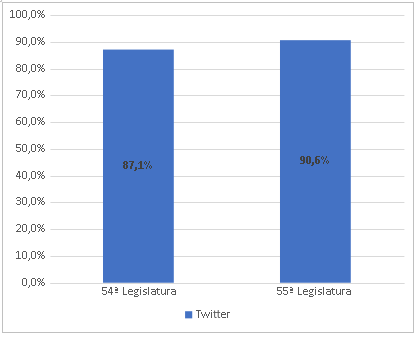
\includegraphics[width=\textwidth]{./imgs/graf2_1.png}
 %\caption{Fonte: Elaboração dos autores.}
 %\end{figure}

Para além da análise de quantos parlamentares possuem contas no Twitter
nas duas legislaturas, percebemos também que houve aumento no número
médio de tweets postados pelos parlamentares, na quantidade de perfis
seguidos por eles e, principalmente, no número médio de seguidores.
Esse aumento de 66\% no volume de seguidores pode
corroborar a ideia de que os eleitores e cidadãos, de forma geral, têm
utilizado os sites de redes sociais digitais como fonte de obtenção de
notícias sociais, econômicas e políticas; e não só como espaços de
interação social (\textsc{cardon}, 2012; \textsc{coutinho \& safatle}, 2009; \textsc{braga \&
carlomagno}, 2014), isto porque ao seguirem os seus representantes eles
podem obter informações sobre decisões que estão sendo tomadas e sobre
as atividades que estão sendo desempenhadas pelos seus parlamentares.

Em relação aos deputados federais da 54ª legislatura, constatamos um número médio de 4.153 tweets, 7.517 seguidores e 1.079 pessoas que seguem.
Para os deputados da 55ª legislatura, os números foram maiores: 5.588 tweets, 11.364 seguidores e 1.257 pessoas que seguem.

%\begin{center}
%Gráfico 2: Número médio de tweets, pessoas que está seguindo e de
%seguidores -- Deputados federais da 54ª e 55ª legislaturas da Câmara dos
%Deputados do Brasil
%\end{center}

 %\begin{figure}[!ht]
 %\centering
 % 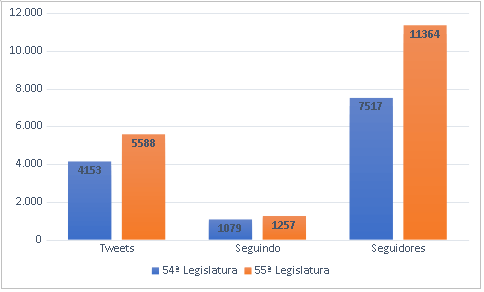
\includegraphics[width=\textwidth]{./imgs/graf2_2.png}
 %\caption{Fonte: Elaboração dos autores.}
 %\end{figure}

% \section{Associações entre o uso do Twitter por parlamentares das 54ª
% e 55ª Legislaturas e variáveis socioeconômicas e políticas}

\section{Twitter e as variáveis socioeconômicas e políticas}

Para além das questões desenvolvidas até aqui procuramos também analisar
a associação de quatro variáveis socioeconômicas e duas variáveis
políticas com o volume de \textit{tweets} postados pelos deputados
federais da 54ª e 55ª legislaturas. As nossas variáveis independentes
são faixa etária, sexo, regiões do Brasil, escolaridade, ideologia e
primeiro mandato.

A nossa variável dependente \textit{número de tweets} foi
construída com base numa decisão estritamente matemática de separar a
frequência dos resultados em quartis (0--25\% das ocorrências no 1º
quartil; 26\% a 50\% no 2º quartil; 51\% a 75\% no 3º quartil; 76\% a
100\% no 4º quartil). Sendo assim, esta variável ficou com os seguintes
recortes em cada uma das legislaturas:

\begin{figure}[!ht]
%\resizebox{\textwidth}{!}{
\begin{center}
\begin{tabular}{|l|l|}
\hline
\textsc{54ª legislatura} & \textsc{55ª legislatura} \\ \hline\hline
1º\,\textsc{q} até 440 & 1º\,\textsc{q} até 500 \\ \hline
2º\,\textsc{q} de 441 a 1.730 & 2º\,\textsc{q} de 501 a 2.275 \\ \hline
3º\,\textsc{q} de 1.731 a 4.630 & 3º\,\textsc{q} de 2.276 a 7.320 \\ \hline
4º\,\textsc{q} acima de 4.631 & 4º\,\textsc{q} acima de 7.321 \\ \hline
\end{tabular}
\end{center}

\caption{Tabela 1: Número de tweets em quartis\footnotemark}
\end{figure}

\footnotetext{Fonte: Elaboração dos autores.}

%\subsection{Variável ``ideologia partidária''}
\subsection{ideologia partidária}

Para o caso brasileiro, a literatura tem afirmado que partidos mais à
esquerda tendem a ter relações mais horizontalizadas e buscam um maior
contato com a sociedade civil (\textsc{avritzer \& navarro}, 2003; \textsc{dagnino}, 2006)
além de utilizarem a Internet e/\,ou as plataformas sociais digitais com
mais intensidade que partidos de direita e centro (\textsc{cruz}, 2011; \textsc{marenco
\& serna}, 2007; \textsc{marques} et al., 2014b).

Utilizamos as categorizações ideológicas de Melo para classificarmos os partidos dentro da variável \textit{ideologia
partidária}. Segundo Melo ``os partidos foram classificados em um
contínuo esquerda"-direita com base em uma média obtida a partir de três
questões contidas no questionário aplicado aos deputados: tomando como
base uma escala de 1 a 10, em que 1 representa a posição mais à esquerda
e 10 a posição mais à direita'' (2011).\footnote{Em Melo (2011) foram
  considerados de esquerda os partidos cuja média obtida ficou entre
  zero e 4 (\textsc{pcdob}, \textsc{psol}, \textsc{pt}, \textsc{pdt} e \textsc{psb}). Foram classificados como de
  centro aqueles situados entre 4,1 e 6 (\textsc{pmdb}, \textsc{psdb}, \textsc{pps}, \textsc{pv}, \textsc{psc},
  \textsc{ptdob}, \textsc{phs}, \textsc{psl}, \textsc{pmn}, \textsc{prb} e \textsc{psdc}). À direita foram posicionados os que
  se situaram acima de 6,0 (\textsc{ptb}, \textsc{pr}, \textsc{dem}, \textsc{pp}, \textsc{ptn} e \textsc{pan}). (\textsc{melo}, 2011).
  Para definirmos o \textsc{psd} e o \textsc{prp} recorremos ao texto de 2000 do mesmo
  autor, que os define como partidos de direita. Por último, em função
  da guinada à direita do \textsc{psc} nos últimos anos, resolvemos desloca"-lo
  para o grupo de partidos à direita.} A categorização:

\begin{itemize}
\item \textbf{Direita} \textsc{ptb, pr, dem, pp, ptn, psd, pen, psc, pros} e \textsc{pmb}.
\item \textbf{Centro} \textsc{pmdb, psdb, pps}, \textsc{pt}do\textsc{b}, \textsc{pv, phs, psl, prb},\\Solidariedade e Rede.
\item \textbf{Esquerda} \textsc{pc}do\textsc{b}, \textsc{pdt, psb, psol} e \textsc{pt} %(\textsc{melo}, 2011).
\end{itemize}

%\begin{center}
%\resizebox{\textwidth}{!}{
%\begin{tabular}{|l|l|}
%\hline
%\textbf{Espectro ideológico} & \textbf{Partidos} \\ \hline
%Direita & \begin{tabular}[c]{@{}l@{}}PTB, PR, DEM, PP, PTN, PSD, PEN,\\ PSC, PROS, PMB\end{tabular} \\ \hline
%Centro & \begin{tabular}[c]{@{}l@{}}PMDB, PSDB, PPS, PTdoB, PV, PHS,\\ PSL, PRB, Solidariedade, Rede\end{tabular} \\ \hline
%Esquerda & PCdoB, PDT, PSB, PSOL, PT \\ \hline
%\end{tabular}
%}

%{\footnotesize\textit{Fonte: Melo (2011) e autores.}}
%\end{center}

Observando a relação entre ideologia e tweets postados temos que, em
média, mais de 60\% dos parlamentares de partidos de esquerda (de ambas
as legislaturas) se enquadram nos quartis de maior volume de
\textit{tweets} (3º e 4º quartis). Em contrapartida, mais de 60\% dos
parlamentares de partidos de direita situam"-se no 1º e 2º quartis. Como
podemos constatar, estes achados corroboram a literatura da área.

\begin{table}
\resizebox{\textwidth}{!}{
\begin{tabular}{lllllllll}
 & \multicolumn{4}{c}{\textsc{54ª legislatura}} & \multicolumn{4}{c}{\textsc{55ª legislatura}} \\ %\cline{2-9} 
 & \multicolumn{4}{c}{\textit{Tweets}} & \multicolumn{4}{c}{\textit{Tweets}} \\ %\cline{2-9} 
 & \begin{tabular}[c]{@{}l@{}}1º\,\textsc{q}\end{tabular} & \begin{tabular}[c]{@{}l@{}}2º\,\textsc{q}\end{tabular} & \begin{tabular}[c]{@{}l@{}}3º\,\textsc{q}\end{tabular} & \begin{tabular}[c]{@{}l@{}}4º\,\textsc{q}\end{tabular} & \begin{tabular}[c]{@{}l@{}}1º\,\textsc{q}\end{tabular} & \begin{tabular}[c]{@{}l@{}}2º\,\textsc{q}\end{tabular} & \begin{tabular}[c]{@{}l@{}}3º\,\textsc{q}\end{tabular} & \begin{tabular}[c]{@{}l@{}}4º\,\textsc{q}\end{tabular} \\ \hline
\textbf{Esquerda} & 12,9\% & 22,4\% & 29,3\% & 35,4\% & 11,7\% & 25\% & 28,3\% & 35\% \\ \hline
\textbf{Centro} & 26,1\% & 23\% & 26,1\% & 24,8\% & 20,1\% & 23,6\% & 28,7\% & 27,6\% \\ \hline
\textbf{Direita} & 35,8\% & 30,7\% & 19\% & 14,6\% & 39,4\% & 26,5\% & 18,8\% & 15,3\% \\ \hline
\end{tabular}
}

\caption{Tabela 2: Ideologia dos deputados federais por número de tweets,
apresentada por quartis de volume.\footnotemark}
\end{table}

\footnotetext{Fonte: Elaboração dos autores.}

\subsection{Faixa Etária}

Em relação à associação entre a adoção do Twitter e a idade dos
parlamentares, a literatura sugere que há uma forte relação invertida,
ou seja, quanto mais velhos, menos presentes e menos interativos na
Internet e nas plataformas de redes sociais (\textsc{lilleker \& michalska},
2011; \textsc{cruz}, 2011; \textsc{marques, aquino \& miola}, 2014a).

No nosso estudo constatamos que os segmentos de maior idade (com 61 anos
de idade ou mais) da 54ª legislatura tinham seus maiores percentuais no
1º quartil. Já na 55ª legislatura esses segmentos \textit{migraram} para o 2º
quartil, tendo havido também um aumento considerável de tweets no quarto
quartil da 55ª legislatura. Ou seja, os parlamentares de maior idade da
55ª legislatura estão \textit{tuitando} mais que o mesmo grupo da 54ª.
Este achado pode ser interpretado como uma adequação ao mundo digital,
mesmo que lenta, por parte dos sexagenários em relação às outras faixas
etárias.

\begin{figure}[!ht]
\resizebox{\textwidth}{!}{
\begin{tabular}{lllllllll}
 & \multicolumn{4}{c}{\textsc{54ª legislatura}} & \multicolumn{4}{c}{\textsc{55ª legislatura}} \\ %\cline{2-9} 
 & \multicolumn{4}{c}{\textit{Tweets}} & \multicolumn{4}{c}{\textit{Tweets}} \\ %\cline{2-9} 
 & \begin{tabular}[c]{@{}l@{}}1º\,\textsc{q}\end{tabular} & \begin{tabular}[c]{@{}l@{}}2º\,\textsc{q}\end{tabular} & \begin{tabular}[c]{@{}l@{}}3º\,\textsc{q}\end{tabular} & \begin{tabular}[c]{@{}l@{}}4º\,\textsc{q}\end{tabular} & \begin{tabular}[c]{@{}l@{}}1º\,\textsc{q}\end{tabular} & \begin{tabular}[c]{@{}l@{}}2º\,\textsc{q}\end{tabular} & \begin{tabular}[c]{@{}l@{}}3º\,\textsc{q}\end{tabular} & \begin{tabular}[c]{@{}l@{}}4º\,\textsc{q}\end{tabular} \\ \hline
\textbf{\begin{tabular}[c]{@{}l@{}}Até 40 anos\end{tabular}} & 17\% & 32,1\% & 22,6\% & 28,3\% & 17,4\% & 32,6\% & 27,9\% & 22,1\% \\ \hline
\textbf{\begin{tabular}[c]{@{}l@{}}41 a 50 anos\end{tabular}} & 20,4\% & 23,5\% & 27,6\% & 28,6\% & 31,6\% & 12,6\% & 30,5\% & 25,3\% \\ \hline
\textbf{\begin{tabular}[c]{@{}l@{}}51 a 60 anos\end{tabular}} & 22\% & 23,8\% & 25,6\% & 28,6\% & 27,9\% & 23,6\% & 23\% & 25,5\% \\ \hline
\textbf{\begin{tabular}[c]{@{}l@{}}61 a 70 anos\end{tabular}} & 33,7\% & 23,5\% & 26,5\% & 16,3\% & 22,1\% & 28,4\% & 21,1\% & 28,4\% \\ \hline
\textbf{\begin{tabular}[c]{@{}l@{}}71 anos ou mais\end{tabular}} & 41,4\% & 31\% & 10,3\% & 17,2\% & 17,4\% & 43,5\% & 21,7\% & 17,4\% \\ \hline
\end{tabular}}

\caption{Tabela 3: Idade dos deputados federais por número de tweets,
apresentada por quartis de volume.\footnotemark}
\end{figure}

\footnotetext{Fonte: Elaboração dos autores.}

\subsection{Sexo}

Em relação à variável \textit{sexo}, mais de 60\% das parlamentares mulheres
estão nos dois grupos de maior volume de \textit{tweets} postados.
Interessante observar que há uma migração, entre as duas legislaturas,
do 3º para o 4º quartil da maior parte das mulheres que \textit{tuitam}.
No caso dos homens, há uma distribuição quase equânime entre os quartis,
mas não há grande variação entre as legislaturas. Comparando os dois
grupos, há proporcionalmente um número maior de mulheres que de homens
parlamentares nos 3º e 4º quartis. Estes achados corroboram os achados
de Marques et al. (2014a) quando analisam a ``tuitagem'' média semanal
entre homens e mulheres e demonstram uma participação maior das mulheres
no Twitter (2014, p.\,185).

\begin{figure}[!ht]

\resizebox{\textwidth}{!}{
\begin{tabular}{lllllllll}

 & \multicolumn{4}{c}{\textsc{54ª legislatura}} & \multicolumn{4}{c}{\textsc{55ª legislatura}} \\ %\cline{2-9} 
 & \multicolumn{4}{c}{\textit{Tweets}} & \multicolumn{4}{c}{\textit{Tweets}} \\ %\cline{2-9} 
 & \begin{tabular}[c]{@{}l@{}}1º\,\textsc{q}\end{tabular} & \begin{tabular}[c]{@{}l@{}}2º\,\textsc{q}\end{tabular} & \begin{tabular}[c]{@{}l@{}}3º\,\textsc{q}\end{tabular} & \begin{tabular}[c]{@{}l@{}}4º\,\textsc{q}\end{tabular} & \begin{tabular}[c]{@{}l@{}}1º\,\textsc{q}\end{tabular} & \begin{tabular}[c]{@{}l@{}}2º\,\textsc{q}\end{tabular} & \begin{tabular}[c]{@{}l@{}}3º\,\textsc{q}\end{tabular} & \begin{tabular}[c]{@{}l@{}}4º\,\textsc{q}\end{tabular} \\ \hline
\textbf{Mulheres} & 18,2\% & 20,5\% & 31,8\% & 29,5\% & 18,2\% & 20,5\% & 27,3\% & 34,1\% \\ \hline
\textbf{Homens} & 25,6\% & 25,6\% & 24,1\% & 24,6\% & 25,7\% & 25,5\% & 24,8\% & 24\% \\ \hline
\end{tabular}}

\caption{Tabela 4: Sexo dos deputados federais por número de tweets,
apresentada por quartis de volume.\footnotemark}
\end{figure}

\footnotetext{Fonte: Elaboração dos autores.}

\subsection{Regiões do Brasil}

Em seu trabalho, Carlomagno (2014) demonstra que mesmo existindo uma
tendência de diminuição das desigualdades regionais em relação ao custo
das campanhas \textit{online} para cargos majoritários, esta fratura digital se
mantém, sendo o Nordeste a região que tinha o menor investimento em
campanhas digitais. Em nosso estudo não há uma grande disparidade no
volume de \textit{tweets} por parlamentar de deputados da região Nordeste
em relação às outras regiões que já esperávamos: Sul, Centro"-Oeste e
Sudeste. A maior disparidade encontrada se deu entre a região Norte e
as outras regiões brasileiras. Há dois achados que consideramos
relevantes: primeiro, os deputados da região Norte \textit{tuitam} bem
menos que os de outras regiões; segundo, apesar de \textit{tuitarem} menos
que seus colegas de outras regiões, constatamos que o somatório dos
percentuais de deputados federais do Norte do país que se enquadram nos
quadrantes de maior volume de \textit{tweets} aumentou um pouco entre as
duas legislaturas analisadas. Por último, os parlamentares da região Sul
foram aqueles que mais \textit{tuitaram}.

\begin{figure}[!ht]
\resizebox{\textwidth}{!}{
\begin{tabular}{lllllllll}
 & \multicolumn{4}{c}{\textsc{54ª legislatura}} & \multicolumn{4}{c}{\textsc{55ª legislatura}} \\ %\cline{2-9} 
 & \multicolumn{4}{c}{\textit{Tweets}} & \multicolumn{4}{c}{\textit{Tweets}} \\ %\cline{2-9} 
 & \begin{tabular}[c]{@{}l@{}}1º\,\textsc{q}\end{tabular} & \begin{tabular}[c]{@{}l@{}}2º\,\textsc{q}\end{tabular} & \begin{tabular}[c]{@{}l@{}}3º\,\textsc{q}\end{tabular} & \begin{tabular}[c]{@{}l@{}}4º\,\textsc{q}\end{tabular} & \begin{tabular}[c]{@{}l@{}}1º\,\textsc{q}\end{tabular} & \begin{tabular}[c]{@{}l@{}}2º\,\textsc{q}\end{tabular} & \begin{tabular}[c]{@{}l@{}}3º\,\textsc{q}\end{tabular} & \begin{tabular}[c]{@{}l@{}}4º\,\textsc{q}\end{tabular} \\ \hline
\textbf{\begin{tabular}[c]{@{}l@{}}Centro-Oeste\end{tabular}} & 23,1\% & 17,9\% & 35,9\% & 23,1\% & 26,3\% & 15,8\% & 31,6\% & 26,3\% \\ \hline
\textbf{Nordeste} & 27,1\% & 25,6\% & 21,8\% & 25,6\% & 29,2\% & 26,9\% & 16,2\% & 27,7\% \\ \hline
\textbf{Norte} & 38,6\% & 31,8\% & 9,1\% & 20,5\% & 43,1\% & 20,7\% & 22,4\% & 13,8\% \\ \hline
\textbf{Sudeste} & 24,7\% & 24,7\% & 25,9\% & 24,7\% & 20,1\% & 29,3\% & 29,3\% & 21,3\% \\ \hline
\textbf{Sul} & 14,3\% & 24,3\% & 31,4\% & 30\% & 13,5\% & 20,3\% & 29,7\% & 36,5\% \\ \hline
\end{tabular}}

\caption{Tabela 5: Região dos parlamentares por número de tweets,
apresentada por quartis de volume.\footnotemark}
\end{figure}

\footnotetext{Fonte: Elaboração dos autores.}

\subsection{Escolaridade}

A literatura pertinente ao tema sugere que a presença \textit{online} também se
correlaciona positivamente com capacidade de apropriação das ferramentas
disponibilizadas na rede e pressupõe que os mais ativos \textit{online} são
majoritariamente jovens e bem"-educados (\textsc{bimber} 2001; \textsc{brundidge and rice},
2010). No trabalho de Marques et al. (2014a), a escolaridade do
eleitorado teve impacto positivo sobre o uso do Twitter (2014, p.\,192). A
partir destas constatações, podemos prever que uma maior escolaridade do
parlamentar aumentaria suas chances de estar conectado e também
aumentaria o número de \textit{tweets}.

\begin{figure}[!ht]
\resizebox{\textwidth}{!}{
\begin{tabular}{lllllllll}
 & \multicolumn{4}{c}{\textsc{54ª legislatura}} & \multicolumn{4}{c}{\textsc{55ª legislatura}} \\ %\cline{2-9} 
 & \multicolumn{4}{c}{\textit{Tweets}} & \multicolumn{4}{c}{\textit{Tweets}} \\ %\cline{2-9} 
 & \begin{tabular}[c]{@{}l@{}}1º\,\textsc{q}\end{tabular} & \begin{tabular}[c]{@{}l@{}}2º\,\textsc{q}\end{tabular} & \begin{tabular}[c]{@{}l@{}}3º\,\textsc{q}\end{tabular} & \begin{tabular}[c]{@{}l@{}}4º\,\textsc{q}\end{tabular} & \begin{tabular}[c]{@{}l@{}}1º\,\textsc{q}\end{tabular} & \begin{tabular}[c]{@{}l@{}}2º\,\textsc{q}\end{tabular} & \begin{tabular}[c]{@{}l@{}}3º\,\textsc{q}\end{tabular} & \begin{tabular}[c]{@{}l@{}}4º\,\textsc{q}\end{tabular} \\ \hline
\textbf{\begin{tabular}[c]{@{}l@{}}Com ensino\end{tabular}} & 24,2\% & 22,5\% & 27\% & 26,2\% & 27,5\% & 35,2\% & 16,5\% & 20,9\% \\ \hline
\textbf{\begin{tabular}[c]{@{}l@{}}Sem ensino\end{tabular}} & 27,5\% & 35,2\% & 16,5\% & 20,9\% & 31,5\% & 32,6\% & 20,2\% & 15,7\% \\ \hline
\end{tabular}}

\caption{Tabela 6: Escolaridade dos parlamentares por número de tweets,
apresentada por quartis de volume. O \textit{ensino} se refere ao ensino superior.\footnotemark}
\end{figure}

\footnotetext{Fonte: Elaboração dos autores.}

Na 54ª legislatura existia diferença entre o volume de \textit{tweets}
postados por parlamentares com e sem ensino superior: 53\% dos primeiros
se encontravam no 3º e 4º quartis, enquanto apenas cerca de 37\% dos
deputados sem ensino superior se encontravam nos mesmos quartis. Já na
legislatura atual, não encontramos uma diferença significativa. Este
achado vai na mesma direção do resultado que encontramos em relação à
variável idade, onde parlamentares mais velhos \textit{tuitavam} menos que
os mais novos na 54ª legislatura e já na 55ª não há mais diferença
relevante entre estes dois grupos.



\subsection{Primeiro Mandato}

Outra hipótese aventada neste trabalho lida com a variável independente
\textit{primeiro mandato}, no qual os novatos teriam um maior número de
tweets que os veteranos. Trata"-se de uma estratégia de comunicação dos
recém"-chegados à casa parlamentar para se contraporem aos parlamentares
com mais de um mandato, e que portanto já possuiriam uma legislatura
consolidada e reconhecida. Algumas pesquisas anteriores têm corroborado
esta hipótese, tais como Marques et al. (2014b).

Segundo nossa pesquisa, entre os deputados da 54ª legislatura
praticamente não há diferenças no volume de \textit{tweets} de deputados
em primeiro mandato e deputados com mais de um mandato. Já na 55ª
legislatura, podemos notar que deputados que estão pelo menos no segundo
mandato estão \textit{tuitando} mais que aqueles que acabaram de chegar
pela primeira vez à câmara federal, ou seja, temos aqui um achado que
vai de encontro à hipótese aventada pelo trabalho de Marques et al.
(2014b).

\begin{figure}[!ht]
\resizebox{\textwidth}{!}{
\begin{tabular}{lllllllll}
 & \multicolumn{4}{c}{\textsc{54ª legislatura}} & \multicolumn{4}{c}{\textsc{55ª legislatura}} \\ %\cline{2-9} 
 & \multicolumn{4}{c}{\textit{Tweets}} & \multicolumn{4}{c}{\textit{Tweets}} \\ %\cline{2-9} 
 & \begin{tabular}[c]{@{}l@{}}1º\,\textsc{q}\end{tabular} & \begin{tabular}[c]{@{}l@{}}2º\,\textsc{q}\end{tabular} & \begin{tabular}[c]{@{}l@{}}3º\,\textsc{q}\end{tabular} & \begin{tabular}[c]{@{}l@{}}4º\,\textsc{q}\end{tabular} & \begin{tabular}[c]{@{}l@{}}1º\,\textsc{q}\end{tabular} & \begin{tabular}[c]{@{}l@{}}2º\,\textsc{q}\end{tabular} & \begin{tabular}[c]{@{}l@{}}3º\,\textsc{q}\end{tabular} & \begin{tabular}[c]{@{}l@{}}4º\,\textsc{q}\end{tabular} \\ \hline
\textbf{Sim} & 23,4\% & 27,5\% & 25,1\% & 24\% & 31,3\% & 31,9\% & 20,9\% & 16\% \\ \hline
\textbf{Não} & 25,8\% & 23,7\% & 24,7\% & 25,8\% & 21,7\% & 21,3\% & 27,3\% & 29,7\% \\ \hline
\end{tabular}}

\caption{Tabela 7: Porcentagem positiva e negativa em relação ao \textit{primeiro mandato} dos parlamentares por número de tweets,
apresentada por quartis de volume.\footnotemark}
\end{figure}

\footnotetext{Fonte: Elaboração dos autores.}

\section{Considerações Finais}

O presente trabalho teve como objetivo inicial analisar
longitudinalmente a apropriação da plataforma de rede social digital
Twitter pelos parlamentares das 54ª e 55ª legislaturas da Câmara Federal
brasileira. Esta análise comparativa poderia nos ajudar a compreender
como os parlamentares estavam se apropriando desta plataforma entre duas
legislaturas e se houve um aumento ou diminuição do seu uso. Constatamos
que houve um aumento tímido no número de parlamentares presentes nesta
plataforma digital --- o aumento foi de apenas 3,49\% --- sendo que mais de
90\% dos deputados federais da 55ª legislatura possuíam perfil no
Twitter.

Além da comparação entre o número de parlamentares que estavam presentes
no Twitter entre as duas legislaturas, procuramos também realizar uma
associação entre o número de \textit{tweets} e algumas variáveis
socioeconômicas e políticas para podermos traçar um perfil dos
parlamentares mais ativos nesta plataforma.

Em relação às associações feitas entre a variável dependente \textit{número de
tweets} e as variáveis independentes socioeconômicas e políticas os
achados do trabalho basicamente corroboram trabalhos feitos
anteriormente. Quando analisamos o número de tweets associado à
ideologia partidária, parlamentares de esquerda \textit{tuitam} mais que o
centro, que por sua vez \textit{tuitam} mais que a direita, sendo que não
há variação do número de tweets entre as duas legislaturas pesquisadas.
Analisamos também a relação entre faixa etária e tweets durante as duas
legislaturas, e constatamos que há uma diminuição de tweets das faixas
etárias de até 40 anos, de 41 a 50 e de 51 a 60, mas em compensação há
um aumento da faixa entre 61 a 70 anos.

A associação entre sexo e número de \textit{tweets} demonstra, primeiro,
que as mulheres parlamentares estão \textit{tuitando} mais do que os
homens. Comparando no tempo o número de \textit{tweets} percebemos que há
uma variação positiva do número de mulheres no quarto quartil, enquanto
que no caso dos homens não há variação.

Ao analisarmos parlamentares das diferentes regiões do país e número de
tweets, os parlamentares da região Sul são os que mais \textit{tuitam} e
parlamentares da região Norte os que menos \textit{tuitam}. Não houve
grandes variações no tempo em relação a parlamentares de diferentes
regiões.

No tocante à variável independente ensino superior constatamos a
existência de uma diferença significativa nos dois últimos quartis
(parlamentares com o maior número de \textit{tweets}) na 54ª legislatura,
sendo que na legislatura seguinte houve praticamente uma equiparação do
número de tweets no 3º e 4º quartis entre parlamentares com e sem ensino
superior.

Por último, quando analisamos a associação entre calouros e veteranos no
parlamento com o número de \textit{tweets}, os veteranos na 55ª
legislatura são os que mais \textit{tuitam}. A hipótese inicial era a de
que os calouros teriam que desenvolver estratégias alternativas de
visibilidade para se contrapor à presença já consolidada e ao
conhecimento por parte da imprensa dos parlamentares antigos da casa.
Esta hipótese não se confirmou. Podemos então supor que os parlamentares
veteranos já tenham uma assessoria organizada no parlamento que gerencie
sua presença nos espaços digitais.

Estudos sobre a apropriação das plataformas de redes sociais digitais
pelos parlamentares federais brasileiros ajudam a compreender as
diferentes estratégias que estes podem desenvolver tendo por objetivo de
estreitar as relações com seu eleitorado, principalmente ao levarmos em
consideração as grandes distâncias destes representantes de suas
\textit{constituencies}. Pudemos constatar com este estudo longitudinal
que há uma tendência clara de termos, com o passar do tempo, todos os
parlamentares federais conectados ao Twitter, independentemente de
condicionantes socioeconômicos ou políticos. As explicações para tal
movimento podem estar relacionadas à percepção por parte da elite
política brasileira da inevitabilidade da ação política nestes espaços
digitais.

\textls[-15]{É preciso reconhecer, no entanto, que sites de redes sociais possuem
arquiteturas distintas e que por isso permitem estratégias diferentes de
relacionamento com os cidadãos. Necessário também reforçar que estamos
tratando de espaços privados que não são nada transparentes e
responsivos, acarretando riscos para os seus usuários que ainda não
estão devidamente analisados pela literatura pertinente. Fica em aberto,
portanto, o desenvolvimento de estudos que comparem não só as diferentes
formas de apropriação das plataformas de redes sociais por parte dos
parlamentares, mas também uma comparação do modelo de negócios destes
ambientes digitais, que acarretam consequências relacionadas à
privacidade, transparência e responsividade.}


\begin{bibliohedra}
\tit{bernardes}, Cristiane. \textsc{leston}-\textsc{bandeira}, Cristina. (2016) ``Information vs
Engagement in parliamentary \textit{websites} -- a case study of Brazil and the
\textsc{uk}''. \textit{Revista Sociologia e Politica} {[}\textit{online}{]}. 2016, vol.\,24,
n.\,59, p.\,91--107.

\tit{bimber}, Bruce. (2001) ``Information and political engagement in America:
the search for effects of information technology at the individual
level''. \textit{Political Research Quarterly}, n.\,54, p.\,53--67.

\tit{braga}, Sérgio Soares. (2007) ``Podem as novas tecnologias de informação
e comunicação auxiliar na consolidação das democracias? Um estudo sobre
a informatização dos órgãos legislativos na América do Sul''.
\textit{Opinião Pública}, Campinas, v.\,13, n.\,1, p.\,1--50.

\titidem; \textsc{nicolás}, Maria Alejandra. (2009) ``The parliament and the
Internet: sociopolitical profile and use of the Internet by the
parliamentary elites of Argentina, Brazil, Paraguay, Uruguay, Venezuela
and Chile''. In: \textsc{ipsa world congress of political science}, 21., 2009,
Santiago. \textit{Anais\ldots{}} Santiago: \textsc{ipsa} World Congress of Political
Science.

\titidem. (2008) ``Prosopografia a partir
da web: avaliando e mensurando as fontes para o estudo das elites
parlamentares brasileiras na Internet''. \textit{Revista de Sociologia e
Política}, \textsc{ufpr}, v.\,16, p.\,107--130.

\tit{brundidge}, Jennifer; \textsc{rice}, Ronald E. (2009) ``Political engagement
online -- do the information rich get richer and the like"-minded more
similar?'' In: \textsc{chadwick}, Andrew; \textsc{howard}, Philip n.\,(Ed.). \textit{The
Routledge Handbook of Internet Politics}. London: Routledge.

\tit{cardon}, Dominique (2012) \textit{A democracia Internet}: promessas e
limites. São Paulo: Forense Universitária.

\tit{cardoso}, Gustavo; \textsc{cunha}, Carlos; \textsc{nascimento}, Susana. (2004) ``Ministers
of parliament and information and communication technologies as a means
of horizontal and vertical communication in Western Europe''
\textit{Information Polity}, v.\,9, p.\,29--40.

\tit{castro}, Mônica Mata Machado de; \textsc{anastasia}, Fátima; \textsc{nunes}, Felipe (2009)
``Determinantes do comportamento particularista de legisladores
estaduais brasileiros''. \textit{Dados},~ rio de Janeiro,~ v.\,52,~n. 4,~p.\,961--1001.

\tit{chadwick}, Andrew. (2006) \textit{Internet politics}: \textit{states,
citizens, and new communication technologies}. Oxford: Oxford University
Press.

\tit{coleman}, Stephen (2010). ``Making parliamentary democracy visible:
speaking to, with, and for the public in the age of interactive
technology''. In: \textsc{chadwick}, Andrew; \textsc{howard}, Philip n.\,(Ed.). \textit{The
Routledge Handbook of Internet Politics}. London: Routledge.

\titidem\mbox{} (2005). ``New mediation and direct representation:
reconceptualizing representation in the digital age''. \textit{New Media
and Society}, n.\,7, p.\,177.

\titidem; \textsc{blumler}, Jay G. (2009) \textit{The Internet and
democratic citizenship} -- \textit{theory, practice and policy}.
Cambridge: Cambridge University Press.

\titidem; \textsc{kaposi}, Ildiko (2009). ``New democracies, news media:
what`s new? A study of e"-participation projects in third"-wave
democracies''. \textit{International Journal of Electronic Governance}, v.\,2, n.\,4, p.\,302--327.

\tit{dagnino}, Evelina, \textsc{olvera}, Alberto, e \textsc{panfichi}, Aldo (orgs.) (2006\textit{)
A disputa pela construção democrática na América Latina}. São Paulo: Paz
e Terra; Campinas: Unicamp.

\tit{davies}, Todd. (2009) ``Introduction''. In: \textsc{davies}, Todd; \textsc{gangadharan},
Seeta Peña (Ed.). \textit{On"-line deliberation}: \textit{design, research
and practice.} Chicago: Center for the Study of Language and
Information. p.\,1--19.

\tit{diamond}, L. (2015) ``Facing up to the democratic recession''. In:
\textit{Journal of democracy} 26, p.\,141--55.

\tit{elvebakk}, Beate (2004) ``Virtually competent? Competence and experience
with Internet"-based technologies among European parliamentarians''.
\textit{Information Policy}, v.\,9, p.\,41--53.

\tit{foa}, R. and \textsc{mounk}, Y. (2016) ``The democratic disconnect''.
\textit{Journal of democracy}, 27. p.\,5--17.

\tit{gibson}, Rachel K.; \textsc{lusoli}, Wainer; \textsc{ward}, Stephen. (2005) ``On"-line
participation in the \textsc{uk}: testing a 'contextualised' model of Internet
effects''. \textit{British Journal of Politics and International
Relations}, v.7. n.4, p.\,561--583.

\tit{griffith}, Jeffrey. \textsc{leston}-\textsc{bandeira}, Cristina. (2012) ``How are
parliaments using new media to engage with citizens''? \textit{The Journal
of Legislative Studies}, v.\,18, n.\,3--4, p.\,496--513.

\tit{gomes}, Wilson. (2005a) ``Internet e participação política em sociedades
democráticas''\textit{. Revista Famecos,} v.\,27, n.\,3, p.\,58--78.

\titidem. (2005b) ``A democracia digital e o problema da
participação civil na decisão política''. \textit{Fronteiras -- Estudos
Midiáticos}, v.\,7, n.\,3, p.\,214--222.

\titidem. (2010) ``Democracia digital: que democracia''? In:
\textsc{miguel}, Luís Felipe; \textsc{biroli}, Flávia (Org.). \textit{Mídia, representação e
democracia}. São Paulo: Hucitec, p.\,241--259.

\titidem. (2011) ``Participação política \textit{online}: questões e
hipóteses de trabalho''. In: \textsc{maia}, Rousiley Celi Moreira; \textsc{gomes}, Wilson;
\textsc{marques}, Francisco Paulo Jamil Almeida. (Org.). \textit{Internet e
participação política no Brasil}. Porto Alegre: Sulina. p.\,19--46.

\titidem. (2009) \textsc{fernandes}, Breno; \textsc{reis}, Lucas; \textsc{silva}, Tarcizio.
(2009) ``Politics 2.0'': Barack Obama's online 2008 campaign.
\textit{Revista de Sociologia e Política}, v.\,17, n.\,34, p.\,29--43.

\tit{hindman}, Matthew (2008) \textit{The Myth of Digital Democracy}. Princeton,
\textsc{nj}: Princeton University Press.

\tit{hoff}, Jens (2004) ``Members of parliaments' use of \textsc{ict} in a comparative
European perspective''. \textit{Information Polity}, v.\,9, p.\,5--16.

\tit{jensen}, Michael J.; \textsc{venkatesh}, Alladi. (2007)'' Government \textit{websites} and
political engagement: facilitating citizen entry into the policy
process''. Irvine: \textsc{crito}, University of California. 
% Disponível em:
% \textless{}http://escholarship.org/uc/item/39f8f9sw\textgreater{}.
% Acesso em: 15 maio 2016.

\tit{karlsson}, M. (2011). ``Interactivity as a strategy for political
representation -- a conceptual discussion and empirical illustrations
among political bloggers.'' Paper prepared for presentation at the
\textsc{ipsa}/\textsc{ecpr} conference ``Whatever happened to North"-South?'' University of
São Paulo"-Brazil

\tit{kies}, Raphäel. (2010) \textit{Promises and limits of web"-deliberation}.
Palgrave: Macmillan.

\tit{leston}-\textsc{bandeira}, Cristina. (2007) ``The impact of the Internet on
parliaments: a legislative studies framework''. \textit{Parliamentary
Affairs}, v.\,60, n.\,4, p.\,655--674.

\tit{levitsky}, S. \textsc{ziblatt}, D. (2018) \textit{Como as democracias morrem}. Rio
de Janeiro: Zahar.

\tit{liff}, Sonia; \textsc{sheperd}, Adrian. (2004) \textit{An evolving gender digital
divide}. In: Oxford Internet Institute, Internet Issue Brief, n.\,2.

\tit{lilliker}, G \& \textsc{michalska}, Karolina Koc (2011) ``\textsc{mep}s online:
Understanding communication strategies for remote representatives''
Darren Paper presented at the European Consortium of Political
Researchers Conference: Reykjavik (Iceland).

\tit{margolis}, Michael; \textsc{resnick}, David. (2000) \textit{Politics as usual}:
\textit{the cyberspace `revolution'}. Thousand Oaks, \textsc{ca}: Sage.

\tit{marques}, F. P. J. A.; \textsc{miola}, E.; \textsc{aquino} J.A. (2014a) ``Parlamentares,
representação política e redes sociais digitais: perfis de uso do
Twitter na Câmara dos Deputados''. \textit{Opinião Pública}, Campinas,
vol.\,20, n.\,2, p.\,178--203.

\titidem. (2014b) ``Deputados
brasileiros no Twitter: um estudo quantitativo dos padrões de adoção e
uso da ferramenta''. \textit{Revista Brasileira de Ciência Política}
(Impresso), v.\,14, p.\,201--225.

\tit{melo}, Carlos Ranulfo. (2000) ``Partidos e migração partidária na câmara
dos deputados''.~\textit{Dados},~Rio de Janeiro, v.\,43, n.2.
%\textit{bit.l\\y/32o4xRJ}

\titidem. (2011) ``\textit{Individualismo e partidarismo em
doze estados brasileiros''}. \textit{Revista Brasileira de Ciências
Sociais}, vol.\,26, n.\,75, p.\,57--71.

\tit{norris}, Pippa. (2001) \textit{Digital divide}: \textit{civic engagement,
information poverty \& and the Internet worldwide}. Cambridge: Cambridge
University Press.

\tit{panagopoulos}, Costas. (2009) \textit{Politicking online -- the
transformation of election campaing communications}. London: Rutgers
University Press.

\tit{perna}, Andrea Sampaio; \textsc{braga}, Sérgio. (2011) ``O lado invisível da
participação política: mecanismos de \textit{e"-participação} e o problema da
gestão da informação nos parlamentos da América Latina''. \textit{Teoria
\& Sociedade} v.\,15, p.\,51--89.

\tit{runciman}, D (2018) \textit{Como a democracia chega ao fim}. São Paulo:
Todavia.

\tit{trechsel}, Alexander H. et al. (2003) \textit{Evaluation of the use of new
technologies in order to facilitate democracy in Europe}. Luxembourg:
European Parliament. 
% Disponível em:
% \textless{}c2d.unige.ch/int/OverviewInstits/Main\_Report\_fi
% nal\%201.pdf\textgreater{}. Acesso em: 15 maio 2016.

\tit{ward}, Stephen; \textsc{gibson}, Rachel. (2009) ``European political organizations
and the Internet: mobilization, participation, and change''. In:
\textsc{chadwick}, Andrew; \textsc{howard}, Philip.\,\textit{Routledge Handbook of Internet
Politics.} New York: Routledge, p.\,25--39.

\tit{wojcieszak}, Magdalena E.; \textsc{mutz}, Diana C. (2009) ``online groups and
political discourse: do online discussion spaces facilitate exposure to
political disagreement''? \textit{Journal of Communication}, v.\,59, n.\,1,
p.\,40--56.

\tit{wright}, Scott. (2012) ``Politics as usual? Revolution, normalization and
a new agenda for online deliberation''. \textit{New Media Society}, v.\,14, n.\,2, p.\,244--261.
\end{bibliohedra}

\chapterspecial{As lideranças políticas brasileiras e as redes
tecnossociais}{}{}

\begin{flushright}
\baselineskip=12pt{\textsc{vera chaia}\\
\textsc{rosemary segurado}\\
\textsc{tathiana chicarino}\\
\textsc{joyce miranda leão martins}}
\end{flushright}


\noindent{}Este artigo é produto de reflexões elaboradas durante o projeto temático
``Lideranças políticas no Brasil: características e questões
institucionais'',\footnote{O projeto temático (nº 12/50987-3)
  ``Lideranças Políticas no Brasil: características e questões
  institucionais'' é financiado pela \textsc{fapesp}. As opiniões, hipóteses e
  conclusões ou recomendações expressas neste trabalho são de
  responsabilidade dos autores e não necessariamente refletem a visão da
  \textsc{fapesp}.} desenvolvido pelos pesquisadores do \textsc{neamp} (Núcleo de Estudos
em Arte, Mídia e Política do Programa de Estudos Pós"-graduados em
Ciências Sociais da \textsc{puc~--~sp}), com financiamento da \textsc{fapesp}. Durante cinco
anos (de 2013 a 2018), a pesquisa teve como foco o entendimento da ação
e a compreensão do exercício da liderança política no território
nacional na atualidade e em outros diversos períodos históricos. Além
desse objetivo, também nos detivemos na observação da ação política
materializada em atores coletivos, suas estratégias, práticas e
finalidades diante de um contexto social e político em transformação
acelerada, influenciado pelas novas sociabilidades que são permitidas
pelas redes tecnossociais.

No que se refere às lideranças políticas, foram realizadas 55
entrevistas semiestruturadas que se caracterizam pela diversidade
regional, partidária e ideológica. Nosso objetivo, neste texto, é
entender o que alguns desses personagens, que são atalhos para a
compreensão de um período e da atuação do campo político, pensam sobre
as redes, observando como a liderança lida com seu exercício (e o
transforma) em tempos nos quais a política também é digital.

Para nossa análise, selecionamos entrevistas de oito lideranças que
julgamos fundamentais para pensar as disputas políticas no Brasil
contemporâneo, polarizado entre a aceitação de projetos de esquerda e
discursos de direita e extrema"-direita: Fernando Haddad, candidato à
presidência da República, em 2018, pelo Partido dos Trabalhadores (\textsc{pt});
Manuela D'ávila, líder do Partido Comunista do Brasil (\textsc{pcdob}) e
candidata à vice"-presidente na chapa petista; Flávio Dino, governador do
Maranhão pelo \textsc{pcdob}; Sâmia Bonfim, deputada federal pelo Partido
Socialismo e Liberdade (\textsc{psol}); João Amôedo, candidato à presidência da
República, em 2018, pelo Partido Novo; Fernando Holiday, deputado
federal pelo Democratas (\textsc{dem}); Major Olímpio, senador do Partido Social
Liberal (\textsc{psl}); e Onyx Lorenzoni (\textsc{dem}), ministro da Casa Civil do governo
Bolsonaro.

O artigo vai se deter na relação dessas lideranças políticas com a
comunicação em duas interações articuladas: com a mídia tradicional e
com sua base eleitoral, a partir das redes. As entrevistas serão
analisadas a partir do método biográfico, entendendo que a articulação
entre construções biográficas e a história, como diria Wright Mills
(1975), proporciona momentos heurísticos para a problematização e
compreensão de processos sociais mais amplos (\textsc{segurado} et al., 2018).

Buscaremos escapar à \textit{ilusio} biográfica, ao sentido linear que os
indivíduos dão às suas trajetórias, compreendendo estas como a ``série
de posições sucessivamente ocupadas por um mesmo agente (ou um mesmo
grupo) num espaço que é ele próprio um devir, estando sujeito a
incessantes transformações'' (\textsc{bourdieu}, 2002, p.\,189). Isto porque, ao
mesmo tempo em que o agente é condicionado pelas estruturas do campo em
que atua, ele também modifica esse espaço.

Em outros termos, os acontecimentos biográficos se definem como posições
e deslocamentos no espaço social, no qual lutas permanentes são travadas
pela aquisição de capital específico, permitindo observar os atores como
produtores e frutos do seu momento. Nesse sentido, o uso das redes
digitais não seria simplesmente a estratégia de atores isolados, mas
consequência da sociedade em rede (\textsc{castells}, 1998) e da democracia de
público (\textsc{manin}, 1995) que transformaram a política, exigindo novos
comportamentos do campo do poder e incidindo sobre o \textit{habitus}, o
qual é definido por Bourdieu (1989) como uma segunda natureza, de origem
social. Nesse trabalho, argumentamos que um novo \textit{habitus} do poder
vem sendo construído na adaptação de estratégias e comportamentos de
políticos ao mundo das redes.

Além da introdução, este trabalho está dividido em outras três partes. A
primeira contextualiza a ambiência midiática da nossa democracia e trata
da emergência das redes tecnossociais nos debates e nas disputas
políticas. Em seguida, é explicada a metodologia e a seleção do
\textit{corpus} da análise. Por fim, na terceira e última seção, são
apresentados os resultados do estudo.

%\section{Metamorfoses no espaço público: a~Internet~como~\textit{lócus}~da~política}

\section{A~Internet~como~\textit{lócus}~da~política}

O espaço público, entendido em uma ampla acepção como o lugar no qual se
desenvolve a ação política, passou, de acordo com Ortega (2011), por
três períodos: o do Iluminismo, no qual o espaço era autônomo e
determinava, em grande parte, a política; o de colonização por parte do
Estado: \textit{partidos políticos y parlamentos son la máxima expresión de lo
público, si bien estas instituciones se entienden (al menos formalmente)
como ámbitos en los que la discusión es siempre accesible al público}
(p.26); o atual, que é constituído pela comunicação midiática, o campo
político e os movimentos sociais, cuja composição foi possível devido a
modificações de natureza diversa, que vão desde outras formas sociais de
fazer política, caso dos novos movimentos sociais, até modificações
radicais nos âmbitos em que acontece a ação política.

Esse espaço, agora estruturado pela comunicação midiática, condicionou a
atuação não apenas das lideranças políticas, mas do próprio governo
representativo, que pode ser descrito como uma ``democracia de público''
(\textsc{manin}, 1995). O tipo ideal \textit{weberiano}, destacado por Manin (1995), marca
a preponderância da imagem das lideranças, nos embates pelo poder.
Escrito em 1995, o texto de Manin dava conta de explicar os efeitos dos
meios de comunicação tradicionais no campo político, em especial, da
televisão. Diante da disputa de imagens, o público seria apenas reativo,
aceitando ou rejeitando as apresentações de si realizadas no palco da
política.

Passados mais de vinte anos do texto escrito por Manin, os avanços da
tecnologia colaboraram para um desdobramento da democracia de público.
As redes tecnossociais emergem como um novo espaço onde a política pode
ser disputada e significada, possibilitando o protagonismo do público
(\textsc{martins}, 2019), antes reativo, e o \textit{ajuste} da imagem das lideranças
que podem utilizar o espaço para falar diretamente ao eleitorado,
explicar mal"-entendidos, culpar a edição jornalística, conseguir novos
adeptos.

Vale destacar que a comunicação mediada é sempre um fenômeno social
contextualizado. Por se constituir em uma materialidade, ou seja, por se
fixar em um substrato material, ``é fácil focalizar o conteúdo simbólico
das mensagens da mídia e ignorar a complexa mobilização das condições
sociais que subjazem à produção e circulação destas mensagens''
(\textsc{thompson}, 1998, p.\,36) ou, mais especificamente, das relações de poder
então constituídas.

A partir do referencial teórico de Castells (2015), podemos ampliar a
discussão para o entendimento de que as relações de poder presentes em
determinada estrutura social possuem um lastro histórico e material, e,
através de processos comunicacionais, são capazes de incidir na
construção de mentalidades coletivas. A própria disputa de poder ocorre
nesse sentido: é realizada para conseguir a adesão de mentes a projetos
de subversão ou manutenção da ordem estabelecida.

Nos distanciando de uma pertinente crítica acerca dos limites da
Internet no que se refere à emancipação dos sujeitos, democratização do
acesso à informação e horizontalidade e descentralização na produção de
conteúdo, tomamos o dito por Castells (2015, p.\,55) que ``tanto o poder
quanto o contrapoder dependem amplamente da batalha sobre a moldagem de
mentalidades realizada no reino das redes de comunicação multimodal''.
Quando há uma reprodução com tendência de manutenção chamamos de poder,
mas se existem tentativas de rompimento desse controle e de sua
institucionalização (daqueles que não veem seus interesses e valores
suficientemente representados) estamos diante de perspectivas de
contrapoder, e, portanto, de disputas por hegemonia nos processos
comunicacionais, sendo estas substancialmente mais eficientes do que os
regramentos coercitivos.

A dinâmica e os efeitos dessas disputas por hegemonia vão depender da
relação dialética entre cultura e tecnologia e a transformação da
realidade, não orientada necessariamente para a sua superação, mas para
a emergência de novas existências e direcionamentos. Nesse sentido,
faz"-se mister o estudo das relações de poder permeadas pelas novas
formas de comunicação.

As redes promovem o encontro \textit{individual} entre político e eleitor, na
transição de uma comunicação de massa de caráter unidirecional para uma
intercomunicação individual que ainda mantém um potencial de alcance de
uma ampla audiência, mas que se caracteriza por uma produção autogerada,
ou seja, o acesso à mensagem é autodirigido e a recepção e recombinação
do conteúdo são autosselecionadas (\textsc{castells}, 2015, p.\,30).

Se, por um lado, a Internet pode abrir caminhos para a construção de
canais que permitam uma democracia mais próxima dos cidadãos, por outro,
pode enfraquecer instituições tradicionais da democracia moderna, que
parecem tornar"-se obsoletas diante da distância do diálogo com o público
e das aspirações destes. Desse modo, a Internet não foi um antídoto real
contra o sistema de comunicação tendencioso, mesmo porque, dirá Castells
(2015), ela poderá incorporar as novas estratégias aprendidas pelos
operadores políticos. Dentre elas, destacamos a manipulação da
informação e a espetacularização da política.

Constituindo"-se como um importante elemento de campanhas eleitorais, a
\textit{digital age} (\textsc{farrel}, \textsc{kolodny} e \textsc{medvic}, 2001) marcou os últimos
pleitos no Brasil, especialmente a partir de 2002 (\textsc{aldé}; \textsc{borges}, 2004).
Conforme sistematização de Penteado (2011), o uso da Internet em
campanhas eleitorais, mais especificamente na elaboração das estratégias
de \textit{marketing} político, contou com três fases:

\begin{enumerate}
\item \textbf{Pré"-moderna} (1945--1984)\quad caracterizada pelo \textit{marketing} político
intuitivo, sem um planejamento rigoroso da campanha, que contava com um
tipo de fazer política na rua, na conversa e na mobilização do corpo a
corpo;

\item \textbf{Moderna} (1985--2002)\quad já contando com os meios de comunicação de massa
na mobilização e na tentativa de persuasão eleitoral;

\item \textbf{Pós"-moderna} (a partir de 2003)\quad contando com um rigor metodológico
mais acentuado na elaboração das campanhas, observa"-se também a
utilização da Internet.
\end{enumerate}

Contudo, se no início foram pouco interativas, mais voltadas para a
divulgação das propagandas e propostas dos candidatos (\textsc{stromer}-\textsc{galley},
2014) e mais episódicas, hoje, observamos duas importantes inflexões. A
primeira delas é a presença da lógica de uma campanha permanente, que
significa a atuação constante do político na tentativa de influenciar a
agenda da mídia e consequentemente a agenda do público. (\textsc{sampaio}, 2016,
p.\,11).

A segunda, que não deixa de se articular com a anterior, diz sobre a
emergência de uma nova fase do \textit{marketing} político digital em que
``o eleitor se torna um personagem ativo na campanha, integrando uma
militância que atua constantemente nas discussões políticas e no
compartilhamento de informações do candidato'' (\textsc{chicarino}; \textsc{segurado},
2019, p.\,9) e tendo como substrato para a formação dessa adesão
político"-ideológica mensagens direcionadas e microssegmentadas. Através
de redes tecnossociais, abre"-se a possibilidade de ``construção de um
candidato customizado, feito sob medida às idiossincráticas expectativas
e necessidades de cada eleitor'' (p.\,9) --- como indica análise da
candidatura à presidência de Jair Bolsonaro.

É para chegar a esse eleitor, agora corresponsável pelas disputas
empreendidas por sua liderança (\textsc{chicarino}, \textsc{segurado}, 2019; \textsc{martins},
2019), que o político precisa buscar meios de tornar seu discurso
atrativo ao mundo das redes, construindo uma imagem de fácil assimilação
e circulação, que possa estar presente em múltiplas plataformas
comunicacionais. Nesse sentido: como as lideranças políticas compreendem
a mídia tradicional e as redes tecnossociais? Antes de apresentar as
respostas encontradas, faz"-se mister apresentar nossa metodologia de
análise.

\section{Metodologia}

Nas pesquisas realizadas dentro do projeto temático ``Lideranças
políticas: características e questões institucionais'', chegamos à
conclusão de que a liderança política, independente do seu tempo
histórico, deve ser vista como produto de uma construção social
relacionada a determinado contexto. É nesse sentido que o método
biográfico aparece como fundamental para análise da ação dos indivíduos
diante dos constrangimentos sociais.

Para escapar da armadilha da \textit{ilusio} biográfica --- o sentido
linear dado pelos indivíduos à sua trajetória --- Bourdieu (1986) dá
algumas pistas. A primeira é lembrar da descoberta do próprio romance
moderno de que ``o real é descontínuo'' (1986, p.\,185). A despeito
disso, Bourdieu (1986) postula a existência de um ``princípio ativo
irredutível'' responsável ``pela unificação das práticas e das
representações'', o chamado \textit{habitus,} a segunda natureza de origem
social (\textsc{bourdieu}, 1989). É desse modo que o mundo social cria formas de
garantir a constância das identidades por meio de instituições de
totalização e unificação do eu.

Uma forma de lidar com a fragmentação constitutiva é por meio da noção
de trajetória, como ``série de posições sucessivamente ocupadas por um
mesmo agente (ou um mesmo grupo) num espaço que é ele próprio um devir,
estando sujeito a incessantes transformações'' (idem, p.\,189).

Os acontecimentos biográficos se definem, portanto, como posições e
deslocamentos no espaço social. As trajetórias seriam essas distintas
posições (que vão desde a militância à obtenção do poder institucional)
em um campo, o qual é definido como o espaço onde lutas permanentes são
travadas pela disputa de posições e aquisição de capital específico. Por
meio dessas lutas e da permanência em um campo, finalmente, há a
aquisição de disposições específicas que formam o \textit{habitus}.

De acordo com Bourdieu (1983), ``para que um campo funcione, é preciso
que haja objetos de disputas e pessoas prontas para disputar o jogo,
dotadas de \textit{habitus} que impliquem no conhecimento e no
reconhecimento das leis imanentes do jogo, dos objetos de disputa etc.''
(p.\,89).

A observação da trajetória das lideranças, dentro do campo do poder,
permite a análise de antigas e novas práticas, bem como a mutação dos
objetos em disputa e dos capitais. Para fazer o \textit{rastreamento} das
biografias e práticas políticas que compõem histórias individuais, mas
não particulares, selecionamentos três distintos momentos das
entrevistas: 

\begin{enumerate}
\item Apresentação do percurso político; 
\item Compreensão da mídia tradicional; 
\item Percepção sobre as redes tecnossociais.
\end{enumerate}

O primeiro momento revela o posicionamento no campo do poder, o lugar do qual
partem as ações que conformam uma biografia; os outros dois permitem
analisar os objetos em disputa, para onde se dirige a liderança (a mídia
é fundamental para a veiculação dos discursos e imagens do poder?;
Importa estar presente nas redes tecnossociais?). A aceitação ou
rejeição das redes permite refletir sobre variações ou permanência do
\textit{habitus} do poder.

O método biográfico, compreendido nessa perspectiva, pode servir para
análises de atores como reveladores de uma época (\textsc{priore}, 2009). Neste
artigo, o utilizamos de modo mais modesto: pretende"-se analisar as
entrevistas comparativamente para que elas joguem luzes no campo
político. Se o bom manejo das redes tecnossociais na difusão de
discursos audiovisuais se torna um novo capital, é porque estamos diante
da emergência de um novo \textit{habitus} político.

\section{As lideranças e as redes tecnossociais}

O ano de 2013 marcou, simultaneamente, o início do nosso projeto
temático\footnote{O contexto do país chegou a dificultar o agendamento
  de entrevistas. As lideranças estavam diante de turbulento momento que
  colaborou para que surgissem novas forças políticas no país e para que
  conhecidos partidos e personagens fossem rejeitados.} e abalo inédito
no sistema político brasileiro: pela primeira vez, milhares de pessoas
saíram às ruas do Brasil a partir de atos marcadas pelas redes
tecnossociais. Governos, partidos políticos e lideranças em geral não
foram poupadas em manifestações que inicialmente tinham como objetivo
protestar contra 20 centavos no aumento da tarifa dos transportes
públicos. Aquele junho marcaria também o fim da hegemonia petista de
controle das ruas. A efetividade da Internet logo serviu para que
diversos movimentos ocupassem as redes, principalmente contra o ciclo
petista no poder, buscando divulgar imagens e discursos de novas
lideranças.

Muitas interpretações são possíveis diante daqueles acontecimentos, mas
um consenso é possível: a democracia brasileira não foi mais a mesma.
Velhas e novas lideranças tiveram que construir seus discursos no
contexto de um país polarizado entre simpatizantes de políticas de
esquerda, de um lado, e de adeptos a discursos de direita e
extrema"-direita, de outro. Intensificando essa divisão nacional,
seguiu"-se ao junho de 2013 um ``terceiro turno''\footnote{Quando o \textsc{psdb} de
  Aécio Neves entrou no \textsc{tse} pedindo recontagem de votos, colocando sob
  suspeição o resultado do pleito que consagrou Dilma Rousseff
  presidente mais uma vez.} da eleição de 2014 e o \textit{impeachment}
de Dilma Rousseff, em 2016.

A Operação Lava Jato,\footnote{Conjunto de investigações em andamento
  pela Polícia Federal Brasileira junto ao Ministério Público com o
  objetivo de investigar desvios na Petrobras. Iniciada em março de
  2014, as mais de 60 fases autorizadas pelo então Juiz Federal Sergio
  Moro, investigaram crimes de corrupção passiva e ativa, gestão
  fraudulenta, lavagem de dinheiro, obstrução de justiça no Brasil e no
  exterior, envolvendo empreiteiras, funcionários da estatal, operadores
  financeiros, além de agentes políticos, principalmente lideranças
  petistas.} em suas mais de 60 fases autorizadas pelo então Juiz
Federal, Sergio Moro, foi a \textit{pá de cal} no sistema político
brasileiro: a imagem da corrupção generalizada levava à rejeição dos que
protagonizavam os tradicionais embates do poder, tornando o contexto
propício para que discursos anti\textit{establishment} conseguissem
adesão.\footnote{É a partir desse contexto que a vitória de Jair
  Bolsonaro, mobilizando redes tecnossociais e líderes de outros campos
  (como o religioso) pode ser entendida.}

Foi pensando nesse cenário que selecionamos para análise as entrevistas
de oito lideranças que representam disputas políticas no Brasil atual e
que tiveram destaque nos desdobramentos posteriores às Jornadas de Junho
de 2013. De um lado, Fernando Haddad (\textsc{pt}), Manuela D'ávila e Flávio Dino
(ambos do \textsc{pcdob}), e Sâmia Bomfim (\textsc{psol}) aliados do projeto petista que
compartilham a trajetória de passagem pelos movimentos sociais; são
defensores de \textit{Lula Livre};\footnote{Movimento que pede a liberdade de
  Lula por considerá"-lo um preso político.} disputaram a eleição
presidencial de 2018 (os dois primeiros como \textit{cabeças de chapa}). Do
outro, uma política que se diz nova, contra os governos Lula e Dilma,
localizados do lado direito do horizonte político e que tem nomes
relacionados aos movimentos de rua verde"-amarelos, conservadores e
liberais: João Amoêdo (Novo), Fernando Holiday (\textsc{dem}), Ônix Lorenzoni
(\textsc{dem}) e Major Olímpio (\textsc{psl}).

À esquerda e à direita, as lideranças políticas ambicionam chegar e
manter"-se no poder, levando adiante suas visões de mundo. Para tanto,
precisam buscar vínculos com seus eleitores e caminhos que possibilitem
tal aproximação. Por isso, não podem ignorar as redes tecnossociais: a
política precisa ir e estar onde estão os que lhe conferem legitimidade.
É nesse sentido que perguntamos: como as lideranças políticas
compreendem a mídia tradicional e as redes tecnossociais? Entendendo
discurso como ação, argumentamos que um novo \textit{habitus} político
pode estar sendo gerado a partir das relações dos políticos com as redes
tecnossociais.

Distante de quaisquer instituições, é possível o uso dos novos espaços
de comunicação para abrir caminhos e promover valores não circunscritos
à política democrática. É nesse sentido que se afirma que as redes tanto
podem abrir caminhos para a construção de canais que permitam uma
democracia mais próxima dos cidadãos como podem enfraquecer a democracia
moderna.

Para responder as questões propostas, parte"-se da análise da trajetória
desses indivíduos, tal como narrada por eles para, em seguida, buscar
aproximações e distanciamentos entre as percepções sobre as mídias em
seus relatos. Foram selecionados os trechos em que as lideranças falam
do início do envolvimento com a política (ponto de partida da
trajetória); o momento em que citam a percepção sobre as redes sociais
(é possível inferir a inflexão de \textit{habitus} político tradicional?);
e a relação que têm com a mídia tradicional. Julga"-se que, havendo
convergências entre distintos polos da política, pode"-se estar em
gestação um novo \textit{habitus} do poder.

Posicionado do lado esquerdo do campo político, partindo de um lugar de
defesa dos últimos governos petistas, Fernando Haddad afirma ter
começado a engajar"-se politicamente nos tempos em que era estudante da
Faculdade de Direito: ``Quem me abordou pela primeira vez para conversar
seriamente sobre política foi o Eugenio Gurti, jornalista; ele estava
montando um grupo político dissidente da \textit{Libelu} na época {[}e{]} eu
vim acompanhando, sempre tive muito interesse no debate político''.

A importância que percebe nas redes tecnossociais, vai além do fato de
serem um espaço onde o eleitorado está: ``é impossível não acompanhar a
rede social hoje {[}\ldots{}{]} porque você tem uma radiodifusão
oligopolizada no Brasil {[}\ldots{}{]}, você tem uma radiodifusão
ideologicamente alinhada, você não tem contradição entre as linhas
editoriais, em geral, muito conservadoras''. Ainda de acordo com Haddad:
``Só muda a linguagem em relação ao público alvo, mas {[}\ldots{}{]} o
sentido da comunicação é o mesmo''

Nesse sentido, as redes sociais são percebidas mais como espaço de
pluralidade de interpretações de fatos, de disputa com a visão de mundo
da mídia tradicional do que de encontro com o eleitor, principalmente
porque ele também aponta ser difícil chegar a determinado público pelas
redes sociais: os mais pobres. Mesmo assim, o político precisa estar nas
redes, nem que seja para fazer circular sua visão de mundo para parcela
específica da população, o ``eleitor Vila Mariana'', pois: ``essas
pessoas que saem de casa 4:30h da manhã e voltam às 22h têm muita
dificuldade, não têm informação, o desafio está nisso, não é difícil
chegar num morador da Vila Mariana as informações, ele tem as
informações''.

Manuela D'ávila, vice de Haddad na disputa à presidência da República em
2018, tem início de trajetória semelhante ao petista: ``Meu pai é
militante social, então durante toda a minha vida eu tive essa ideia de
ser de esquerda, de ser militante, mas foi no movimento estudantil que
eu consegui organizar isso em torno de um ideário, de um partido, né''.

Sua percepção da mídia tradicional está vinculada a um comportamento
específico da mídia pelo fato de ela ser uma mulher na política: ``Eu
cheguei em Brasília e me deram um espaço gigantesco, machista, de musa
do congresso. Para mim é negativo ser musa {[}\ldots{}{]} porque eu não
concorria a miss''. Ela tem, também, um entendimento semelhante ao de
Haddad: ``Existe o oligopólio, tem pauta, tem estudo, então a gente''\ldots{}

Manuela sinaliza que não apenas a política encontrou outro espaço de
contato com os eleitores, como também que, a partir desse espaço, o
campo do poder vai conseguindo modificar pautas dos meios de comunicação
tradicional: ``Hoje, eu consigo ser uma liderança que tem o seu espaço
pra dar as suas opiniões cotidianamente, mesmo que não me chamem para
programa nenhum de rádio. Não é o mesmo volume, mas tu vai construindo,
tu vai alterando as pautas''. D'ávila lembra de um caso relevante: ``A
pauta de gênero no governo Temer, eu recebi num grupo, eu escrevi no
Twitter e duas jornalistas já me escreveram ``nossa que pauta
boa'', certo? Um dia antes da posse. Então, não surgiu de graça dos
grandes meios''.

A líder do \textsc{pcdob} destaca ainda a mudança percebida no comportamento
dos eleitores: ``Isso empodera as pessoas, porque as relações de poder
elas também são relações de como a gente se comunica, das coisas que a
gente utiliza uns para os outros e de quem diz, de quem é o portador da
mensagem, a Internet permite que a gente tenha vários emissores''.

A observação de D'ávila merece destaque por fazer parte de um
desdobramento da democracia de público descrita por Manin (1995): o
ativismo nas redes marca a marginalização do papel reativo de eleitoras
e eleitores, que passam a participar do jogo político"-eleitoral também
produzindo imagens e visões de mundo que podem afetar as disputas
tradicionais do poder (\textsc{martins}, 2019).

Do mesmo partido de Manuela, Flávio Dino, governador do Maranhão e nome
de destaque do campo progressista, desafiou a hegemonia da família
Sarney no estado já em 2014 quando vence o candidato \textit{sarneysista} Lobão
Filho. Em 2018, disputa diretamente com Roseana Sarney, filha do
ex"-presidente, e a vence, repetindo o embate de 2010, mas com um
resultado diferente.

Importante destacar que a família Sarney detém o controle dos principais
meios de comunicação maranhenses, um contexto que, entre outros motivos
tal qual a mudança na esfera pública como já abordamos, levou o
governador ``a utilizar as ferramentas digitais em seu mandato {[}\ldots{}{]}
mesmo governando um estado em que o acesso à Internet está bem abaixo da
média nacional'' (\textsc{massuchin}; \textsc{silva}, 2019, p.\,231).

Esse contexto vem à tona na fala de Dino, com uma visão sobre a mídia
tradicional que se aproxima daquela expressada por Haddad e D'ávila. O
político afirma que ``no caso do estado, a gente lida com uma
dificuldade, que é a propriedade dos meios de comunicação. O principal
meio de comunicação, o império midiático, é na verdade um partido
político de oposição''. Uma fração dessa mídia, que ele diz ser mais
comercial, acompanha o governo, que procura marcar presença nesses
veículos. O principal meio de comunicação da sua gestão, entretanto, é o
Twitter: ``Digamos que o canal oficial é o Twitter, onde
desde cedo até de noite eu vou verbalizando o discurso do governo e tal.
E permitindo que pelo menos uma rede de opinião pública que tem acesso à
Internet acompanhe as ações de governo''. Sua trajetória também é
semelhante a das duas primeiras lideranças:

\begin{quote}
Comecei a atuar politicamente mais ou menos com 15 anos de idade, no
movimento estudantil secundarista da época, isso em 1983, quando nós
estávamos constituindo, ou reconstituindo as entidades de âmbito
nacional, a \textsc{umes} e \textsc{ubes} haviam sido recentemente reinstauradas, após a
longa noite da ditadura, e eu participava aqui no Maranhão, desses
movimentos, aqui, de reorganização da juventude. E participei depois,
também, em continuidade, no movimento estudantil da Universidade Federal
do Maranhão.
\end{quote}

Assim, para aqueles que começaram a trajetória nos movimentos sociais de
esquerda, construindo suas bases eleitorais a partir da militância e
dentro de instituições estudantis, as redes tecnossociais emergem como
um novo \textit{lócus} de resistência ao poder estabelecido, aos
conservadores, à direita. Os palcos dos comícios de rua e as campanhas
tradicionais não podem ser mais os únicos modos de se conectar ao
eleitorado e buscar mobilizá"-lo. É preciso adequar"-se à linguagem e à
lógica das redes, modificando atuações e interação com os eleitores.

Como é o caso de Sâmia Bomfim, que inicia a sua militância no movimento
estudantil que integrou na Universidade de São Paulo (\textsc{usp}), antes mesmo
de sua filiação ao \textsc{psol}, em 2011. Na esteira das Jornadas de Junho de
2013 e da polarizada eleição de 2014, começa a militar mais intensamente
no movimento feminista, quando, de acordo com ela, participou ``dessas
marchas contra o Eduardo Cunha e contra a cultura do estupro, sempre com
essa conexão das ruas e das redes sociais''.

Eleita em 2016 para o cargo de vereadora da cidade de São Paulo, Sâmia
integrou uma frente eleitoral auto"-organizada que buscava encampar
candidaturas de jovens progressistas em um misto de ativismo e
institucionalização, impulsionando

\begin{quote}
{[}\ldots{}{]} O quesito participação nas propostas e candidaturas, apostando
numa representação política coletiva, do jovem"-usuário, desenganado e
desconfiado politicamente, com o jovem"-ativista e o jovem"-candidato,
estimulados a usar o grande alcance e possibilidade de comunicação mais
horizontalizada dessas mídias para apresentação de seus ideais políticos
e suas propostas (\textsc{lobo}, 2017, p.\,264).
\end{quote}

Nesse sentido diz que se não tivesse feito parte da Bancada Ativista em
2016 talvez não tivesse sido eleita, ``porque ela virou uma espécie de
um cardápio de candidaturas de lideranças e tal. E teve outras \textit{offline},
Me Representa e coisas do tipo.\footnote{No pleito de 2016 tivemos as
  experiências das plataformas Me Representa e Vereadores Que Queremos,
  a co"-vereança na cidade de Alto Paraíso, em Goiás, e a Gabinetona de
  Belo Horizonte, que a partir de um coletivo chamado \textsc{muitas} conclamou
  uma filiação em massa no \textsc{psol} resultando em 12 candidaturas, duas
  delas bem"-sucedidas. Além disso, em 2018 a candidatura da Banca
  Ativista é vitoriosa à Câmara Estadual de São Paulo, não mais como uma
  plataforma que agrega diferentes candidaturas, mas como uma
  candidatura coletiva com nove \textit{codeputados}.} Eu acho que são importantes, pra renovar a
política, pra ter novas figuras''.

  % Ver mais em:
  % \textit{www.cartacapital.com.br/politica/quais-sao-as-novas-formas-de-arejar-a-representacao-politica}
  % Acesso em set. 2019.

Em 2018, a política seria novamente eleita, mas agora ao cargo de
deputada federal. Falando sobre comunicação com a base eleitoral, ela
afirma que, talvez:

\begin{quote}
Seja um dos principais pilares do nosso mandato, tentar utilizar todas
as redes sociais possíveis que existem, Instagram, Twitter, Telegram,
Facebook, enfim tudo o que já foi inventado {[}\ldots{}{]} porque foi sempre
assim que eu construí política, criando a própria narrativa, fazendo uma
própria comunicação, porque se eu for depender dos meios tradicionais eu
não vou conseguir muitas coisas, enfim, acho que o nosso espaço é um
pouco esse na sociedade.
\end{quote}

O caso de Sâmia é paradigmático para o argumento que estamos
desenvolvendo. Vinda da esquerda e dos movimentos sociais, mas em
momento em que o campo político passa a ter como capital o bom manejo do
uso das redes, sua liderança é forjada entre o mundo das ruas e das
redes, indicando que uma nova natureza, um novo \textit{habitus} de
políticos neófitos vem a ser incorporado na atenção ao mundo conectado,
eternamente \textit{online}.

Do lado à direita do campo político, João Amoêdo diz nunca ter pensado
em entrar para a política. Esteve sempre na iniciativa privada,
valorizando o indivíduo e suas ações particulares. Foi um amigo, da
administração do Unibanco, que o apresentara a políticos, pois pensava
em levar para o mundo público práticas da administração privada. De
acordo com Amoêdo: ``quando eu me defrontei com algumas pessoas
{[}\ldots{}{]} eu achei que eram líderes que não inspiravam, que não tinham o
\textsc{dna} necessário para uma boa gestão e, consequentemente, sem um bom
líder, você, dificilmente, monta uma boa equipe''. A partir daí teria
surgido a ideia de montar um partido e de atrair novas lideranças para a
legenda.

A sigla foi fundada em 2011, mas se tornou mais conhecida depois que o
próprio João se tornou candidato à presidência em 2018, conseguindo
atrair atores vinculados a muitos grupos pró"-\textit{impeachmen}t, tais
como o Vem pra Rua, \textsc{mbl}, Renova \textsc{br}.

Amoêdo considera boa sua relação com a mídia, mas acredita que existe um
``questionamento muito grande de quem entra na política, talvez pelo
histórico passado, às vezes, eu tenho a sensação que o pressuposto é: se
a pessoa entrou na política, alguma coisa de errado tem''.

As redes tecnossociais, de acordo com ele, são o principal canal de
comunicação com os eleitores: ``O Novo é muito ativo, hoje é o maior
partido nas mídias sociais, principalmente no Facebook, então a
gente usou muito, porque é uma forma barata de acessar as pessoas, é uma
forma interessante também de interagir''.

No caso dessa liderança, não se percebe uma transformação de um
\textit{habitus} político, porque ela não era desse campo, ao contrário,
menospreza a política tradicional: ``A política tem uma dinâmica que nós
não gostamos, é a dinâmica da perpetuação do poder, é a dinâmica dos
interesses privados acima dos interesses públicos, é a dinâmica dos
caciques, das lideranças, é dinâmica da falta de instituições''.
Infere"-se, então, que sua própria entrada no campo do poder ocorre
porque as vias de acesso mudaram: não são necessários a aproximação a um
partido, a movimentos sociais ou mesmo ser de uma família de políticos.
A adesão a um discurso difundido pelas novas mídias, com a ajuda do
eleitorado, torna"-se um capital.

Apesar de parecer pouca a porcentagem que Amoêdo obteve na eleição
presidencial de 2018 (2,5\%), vale destacar que sua adesão foi maior do
que a de Marina Silva (1\%), que iniciou seu percurso pelas batalhas do
poder ainda jovem, foi uma das fundadoras da Central Única dos
Trabalhadores (\textsc{cut}), no Acre, e ex"-ministra dos governos Lula.

Conhecido e eleito com a ajuda das redes tecnossociais, Fernando
Holiday, do \textsc{mbl} e do \textsc{dem}, tem em comum com Amoêdo, para além de valores
mais à direita do espectro político (como a ênfase no indivíduo), o fato
de nunca ter pensado em se tornar político. De acordo com ele: ``Nunca
pensei em ser político ou participei de algum movimento {[}\ldots{}{]} até
que, final de 2014, eu comecei a gravar alguns vídeos expondo meus
posicionamentos. {[}\ldots{}{]} Eu me tornei uma figura conhecida, com
seguidores na Internet''.

Os vídeos de Holiday foram colocados na plataforma do Movimento Brasil
Livre, na época um pequeno movimento, e falavam contra as cotas raciais.
Para Holiday, a mídia tradicional: ``Não entendeu as mudanças pelas
quais a sociedade passou, não só aqui no Brasil, nos Estados Unidos nas
eleições americanas nós vemos isso também, um questionamento daquilo que
vem da mídia tradicional''. Além disso: ``A mídia, ela não consegue
acompanhar a velocidade das mudanças {[}\ldots{}{]} falha na interpretação
dos acontecimentos''.

Tal como Fernando Haddad, Fernando Holiday percebe um viés ideológico na
mídia, mas em sentido oposto: ``Muitos dos jornalistas, {[}\ldots{}{]} a
grande maioria sem sombra de dúvidas não aceita qualquer ideia, não é
adepta a qualquer ideia que não seja de esquerda. {[}\ldots{}{]} Saem das
universidades e vão para as redações dos grandes jornais, já saem com um
viés''. Enquanto o foco do petista recai nas empresas, o do liberal
recai sobre os indivíduos.

Holiday acredita que as redes tecnossociais ``passam a ser uma fonte
para as pessoas que cansaram dos grandes jornais, dos grupos de
comunicação, mas também acaba sendo um pouco perigosa. Às vezes, surgem
as chamadas \textit{fake news}, notícias falsas''. Daí, surge o que ele
considera o principal desafio para a sociedade atual, em relação à
mídia, e os principais desafios para as novas lideranças políticas:
``encontrar um equilíbrio que permita uma visão realista e não
distorcida como a oferecida pelas mídias tradicionais''.

Político fundamental na ascensão do bolsonarismo, Major Olímpio foi
policial militar por 29 anos, e, embora diga que não é apoiado pelas
entidades de classe da Polícia Militar, tampouco pelo comando da
polícia, ``talvez eu seja muito apoiado pelo policial, do soldado ao
coronel''.

Por conta de um temperamento tempestivo e questionador, segundo ele
próprio, foi punido algumas vezes até o momento em que decidiu seguir a
carreira de político profissional sendo eleito deputado federal pelo
estado de São Paulo em 2006.

De nossos entrevistados é o único que não faz uma crítica contundente à
imprensa, que diz ter um profundo respeito pela imprensa, ``eu gosto
mais de comunicação do que gosto de política''. Segundo ele, não é um
político midiático porque é ``muito previsível o que eu vou fazer, como
eu vou votar''.

Sobre as redes tecnossociais diz ser o campo de maior atuação no que se
refere ao engajamento de eleitores e apoiadores:

\begin{quote}
De todas as ordens, de todos os segmentos {[}\ldots{}{]} não é só de
policiais, não é só de militares, não é só de servidores públicos. Houve
um momento que eu manifestei de forma mais contundente de forma não
ensaiada a minha indignação que foi o dia em que a Dilma queria dar
posse ao Lula para dar um salvo"-conduto para ele que eu fui na cerimônia
mesmo, não combinei, se eu tivesse que combinar, ia combinar com
imprensa e tal, e realmente eu fui dizer, e sai gritando que aquilo era
uma vergonha aquilo tudo. Aí aquilo acabou despertando, na minha fala,
um sentimento de indignação de muita gente da população brasileira,
então tem grupos aqui do Brasil todo, a maioria do estado de São Paulo,
mas eu tenho a minha forma de comunicação, veja as minhas manifestações
em plenário, eu, eventualmente, em vídeos caseiros que nós gravamos aqui
no próprio celular, é a minha forma de comunicação mesmo.
\end{quote}

Diferente de Amoêdo e Holiday, e de certa forma de Major Olímpio, Onyx
Lorenzoni não é uma liderança nova, mas também surfa nas ondas do
antipetismo e da Internet. Ele entrou na política no final da década de
1980, em suas palavras, ``Por conta de uma liderança profissional. Eu
sou veterinário e era presidente do sindicato dos veterinários do Rio
Grande do Sul''. Tal como Haddad e Holiday, Lorenzoni percebe um viés na
mídia. De maneira semelhante ao segundo Fernando, percebe um problema na
formação dos jornalistas: ``muitas vezes, a minha informação, até por eu
ser um liberal, acaba entrando em confronto com a informação média dos
jornalistas brasileiros, que durante longuíssimo tempo teve uma
influência muito grande do pensamento marxista''.

Para ele, o Brasil está em um momento no qual os grandes meios de
comunicação ``não fazem mais a cabeça das pessoas'', que formam a
própria opinião e se tornam ativistas a partir da Internet: ``Hoje, tu
tens milhões de pessoas no Brasil que tem ativismo político sem ter
ligação com partido, sem ter ligação com nenhum agente público''. Essa
participação do público em novos espaços comunicacionais (como Manuela
D'ávila também apontou) mudaria a configuração da própria política
brasileira: ``Nós vamos ter uma renovação como nunca houve no Brasil,
vai ser uma renovação muito intensa {[}\ldots{}{]}, e acredito que vão surgir
daí novos movimentos que vão levar a criação de novos partidos''. Essa
mudança seria estimulada também pela legislação que ``será restritiva à
ação partidária, o fato da cláusula de barreira, cláusula de desempenho.
A proibição de coligações a partir de 2020, ela vai criar outra
realidade''.

Onyx Lorenzoni, Fernando Haddad, Flávio Dino, Manuela D'ávila, Sâmia
Bomfim, Major Olímpio, Fernando Holiday e João Amoêdo, lideranças à
esquerda e à direita do campo político, fazem uso das redes
tecnossociais e as consideram \textit{lócus} privilegiado de acesso a
eleitoras e eleitores. Os políticos que possuíam um dos \textit{habitus}
tradicionais da política, forjado na luta dentro dos movimentos sociais,
adaptam seus discursos e outras ações à lógica do \textit{mundo virtual}.
Novos políticos adentram no campo do poder e chamam a atenção do
eleitorado porque outro capital vem sendo formado: o bom manejo das
redes. Se alguém consegue chegar ao público por essa via, torna menos
fundamental o papel dos movimentos, dos partidos tradicionais ou da
televisão.

A rejeição da mídia tradicional, por outro lado, mostra que essa já não
é mais a principal preocupação dos políticos em um contexto no qual
discursos dos meios de comunicação são mais facilmente questionados e
negados. Devido a essa constatação, o receio é como chegar a todas as
parcelas do eleitorado através das redes ou como conseguir conectar"-se
diariamente. A abordagem qualitativa (e o número pequeno de casos
analisados neste artigo) não permite generalização, mas evidencia que um
novo \textit{habitus} pode estar sendo gerado no campo do poder.

\section{Conclusão}

A simbiose entre política e mídia, atravessando antigas práticas,
representa ``a cristalização, no campo político, de uma transformação
que, ao alastrar"-se por inúmeras esferas do cotidiano, já transformou as
sociedades contemporâneas mais complexas em 'sociedades midiáticas'"
(\textsc{ribeiro} 2004, p.26). A metamorfose no espaço público incidiu no campo
do poder e provocou transformações no próprio governo representativo,
permitindo a percepção, em meados da década de 1990, de uma ``democracia
de público'' (\textsc{manin}, 1995), na qual a disputa das imagens das lideranças
políticas ganhou preponderância diante de partidos e ideologias,
desenvolvendo"-se nos meios de comunicação para ganhar adesão ou rejeição
do público, apenas reativo diante dos espetáculos do poder.

Com novos avanços na tecnologia, que possibilitaram a multiplicidade de
espaços midiáticos, o público, antes apenas receptor de mensagens, passa
a ser também emissor, produtor de imagens públicas, corresponsável pelas
disputas político"-eleitorais de suas lideranças (\textsc{chicarino}, \textsc{segurado},
2019; \textsc{martins}, 2019). Nesse contexto, os políticos vão às redes para
chegar ao eleitorado; divulgar suas imagens públicas; difundir discursos
que possam ser veiculados sem a interferência da mídia tradicional. Ao
analisar a compreensão de oito lideranças sobre a mídia tradicional e as
redes tecnossociais obtivemos material empírico que fortalece o
argumento de que estamos diante da emergência de um novo \textit{habitus}
do poder.

Personagens com distintas trajetórias e posicionados em polos opostos do
horizonte político percebem nas redes um \textit{lócus} de divulgação da
política, difusão de visões de mundo, conquista da adesão de eleitores e
eleitoras. Também convergem na percepção de que a mídia limita a
compreensão da política, seja porque é um oligopólio (caso das
interpretações à esquerda), seja porque tem perspectiva enviesada
(percepções de lideranças à esquerda e à direita) ou porque os
jornalistas já não compreendem que a realidade mudou (como afirmou
Holiday). A medida em que a mídia tradicional é vista com menor
importância (aqui não estão incluídas as propagandas partidárias
televisivas), a Internet aparece como fonte maior de esperança, meio que
interessa ao poder estabelecido e ao contrapoder, dependentes que são da
moldagem de mentalidades, para lembrar Castells (2015). As falas
evidenciam que comportamentos, estratégias e ações estão sendo
modificados em espaço no qual o eleitorado pode ser disputado sem
filtros e edições jornalísticas, a partir de maior interação.

As visões de mundo produzidas por distintos emissores transformam as
relações tradicionais entre mídia, política e votantes, obrigando o
campo do poder a adequar"-se para a busca de um novo capital político: o
bom manejo das redes teccnossocias. É nesse sentido que um novo
\textit{habitus} emerge: políticos e políticas incorporam novos modos de
falar, de captar a atenção do público, de disputar o poder, almejando
permanecer sempre \textit{online} na sociedade conectada.


\begin{bibliohedra}
\tit{aldé}, A.; \textsc{borges}, J. \textit{Internet, imprensa e as eleições de 2002}:
pautando notícia sem tempo real. Logos, Rio de Janeiro, n.\,21. 2004.

\tit{alonso}, Angela. \textit{A Política Das Ruas}: Protestos em São Paulo de
Dilma a Temer. Novos Estudos. \textsc{cebrap}. São Paulo, ed. Especial, Jun/2017,
p.\,49--58.

\tit{castells}, Manuel. \textit{O poder da comunicação}. São Paulo: Paz e
Terra, 2015.

\tit{chicarino}, T.S.; \textsc{segurado}, R. \textit{Um candidato customizado}: as
eleições presidenciais de 2018 e o papel das redes tecnosociais.
Cadernos Adenauer \textsc{xix} (2019), n.\,1. Eleições 2018 e perspectivas para o
novo governo. rio de Janeiro: Fundação Konrad Adenauer, abril 2019.

\tit{bourdieu}, Pierre. \textit{O poder simbólico}. rio de Janeiro: Bertrand
Brasil, 1989.

\tit{farrell}, David M; \textsc{web}, Paul. \textit{Political Parties as Campaing
Organization}. In. \textsc{dalton}, R; \textsc{wattenberg}, M. (\textsc{ed}s.). Parties without
Partisans: political changes in advanced industrial democracies. 1ª Ed.
Oxfor University Press, 2002.

\tit{gramsci}, Antonio. \textit{Maquiavel}. A política e o Estado Moderno. Rio
de Janeiro: Civilização Brasileira, 1968.

\tit{lobo}, Denis Carneiro. \textit{Coletivos organizados para mudar o perfil
das câmaras municipais no Brasil:} jovens, política, plataforma e redes
sociais. In: Fernandes, Carla Montuori; Oliveira, Luiz Ademir De; Chaia,
Vera. Comunicação política e estratégias de campanha. Rio de Janeiro:
Multifoco, 2017. p.\,257--280.

\tit{manin}, Bernard. As metamorfoses do governo representativo.
\textit{Revista Brasileira de Ciências Sociais}. v.\,10, n.\,29, p.\,5--34,
outubro, 1995.

\tit{martins}, Joyce Miranda Leão. O protagonismo do público: Bernard Manin e
a eleição presidencial de 2018. \textit{Agenda Política}, v.\,7, n.\,2,
2019.

\tit{massuchin}, Michele Goulart; \textsc{silva}, Luana Fonseca. \textit{Campanha
permanente nas redes sociais digitais}: um estudo de caso da análise da
fanpage do governador Flávio Dino, no Brasil. Revista Internacional de
Relaciones Públicas, n.\,17, vol.\,\textsc{ix}, 2019.

\tit{penteado}, Claudio. \textit{Marketing político na era digital}:
perspectivas e possibilidades. Revista \textsc{usp}, 2011, 90: 6--23.

\tit{pomian}, Krzysztof. \textit{A História das Estruturas}. In: \textsc{le} \textsc{goff},
Jacques (org.) A História Nova. São Paulo: Martins Fontes, 2005.

\tit{priore}, Mary del. Biografia: quando o indivíduo encontra a história. Rio
de Janeiro, \textit{Topoi}, v.\,10, n.\,19, p.\,7--16, 07--12/2009.

\tit{ribeiro}, Pedro José Floriano. Campanhas eleitorais em sociedades
midiáticas: articulando e revisando conceitos. \textit{Revista
Sociologia e Política}, n.\,22, 2004.

\tit{sampaio}, Thiago. \textit{A mídia e a campanha permanente}: a disputa
pela atribuição de responsabilidade no primeiro mandato da presidente
Dilma Rousseff (2011--2014). In: Anais 10º Encontro \textsc{abcp}, 2016.

\tit{segurado}, Rosemary; \textsc{malina}, Pedro; \textsc{chicarino}, Tathiana Senne; \textsc{martins},
Joyce Miranda Leão. Mulheres na política: atuações institucionais e
partidárias no espectro da esquerda. In: Segurado, Rosemary; Almeida,
Rodrigo Estramanho; Chaia, Vera (Orgs.). \textit{Política e liderança}:
teorias e práticas. São Paulo: \textsc{puc~--~sp}, 2018. p.\,64--75.

\titidem\mbox{} et al. \textit{Impeachment de Dilma Roussef e o
debate no Twitter.} Aurora: revista de arte, mídia e política, São
Paulo, v.\,9, n.\,30, p.\,200--224, 10/2017--01/2018.

\tit{solano}, Esther. \textit{Crise da Democracia e extremismos de direita}.
Friedrich Erbert Shiftung Brasil. São Paulo. 

% Disponível em:
% http://library.fes.de/pdf-files/bueros/brasilien/14508.pdf, 2018. Acesso
% em: 10 out. 2018.

\tit{stromer}-\textsc{galley}, Jennifer. \textit{Presidential campaigning in the
Internet age}. Oxford University Press, 2014.

\tit{thompson}, John B. \textit{A mídia e a modernidade}. Uma teoria social da
mídia. Petrópolis: Editora Vozes, 1998.


\section{Anexo: As entrevistadas e entrevistados\protect\footnote{As
  trajetórias das lideranças entrevistadas constam em um instrumento de
  pesquisa, nomeado de \textit{bioficha}, que contém formulários
  organizados segundo parâmetros pré"-definidos, para a composição do
  quadro geral de lideranças políticas brasileiras. Essas informações
  serão disponibilizadas ao público em geral. Para saber mais acesse
  \textit{pucsp.br/neamp/}.}}

\paragraph{Fernando Haddad} Ingressou na Faculdade de Direito do Largo São Francisco da \textsc{usp} em 1981.
Durante a graduação, fez parte da militância estudantil, tendo se
filiado ao \textsc{pt} em 1983, e eleito presidente do Centro Acadêmico \textsc{xi} de
Agosto em 1984. Formou"-se em 1985, especializando"-se em Direito Civil.
Completou seu mestrado em Economia (\textsc{usp}) em 1990 e o doutorado em
Filosofia (\textsc{usp}) em 1996. Em 1997, foi aprovado no concurso para
professor da \textsc{usp}, no departamento de Ciência Política.

Assume seu primeiro cargo político em 2001 como chefe de gabinete na
secretaria de Finanças e Desenvolvimento Econômico da cidade de São
Paulo, sob o comando de João Sayad, durante a prefeitura da Marta
Suplicy (\textsc{pt}), cargo que ocupou até 2003 quando é nomeado assessor
especial do Ministério do Planejamento, Orçamento e Gestão comandado por
Guido Mantega. No ano seguinte, foi promovido ao cargo de
Secretário"-Executivo do Ministério da Educação, na gestão de Tarso
Genro. Torna"-se Ministro da Educação do Governo Lula em 2005, como
ministro, Haddad desenvolveu o Prouni, com vistas a expandir o acesso à
universidade. Em sua gestão, também alterou as regras do Fundo de
Financiamento ao Estudante do Ensino Superior (\textsc{fies}).

Tornou"-se Prefeito da cidade de São Paulo em 2012, durante a presidência
de Dilma Roussef. Concorreu à reeleição à prefeitura de São Paulo em
2016, tendo sido derrotado por João Dória (\textsc{psdb}) ainda no 1º turno. O
mesmo ocorreu na eleição para a presidência da República em 2018, sendo
derrotado por Jair Bolsonaro no 2º turno.

\paragraph{Manuela D'ávila} Oriunda do rio Grande do Sul, Manuela D'Ávila inicia sua trajetória
política no movimento estudantil, mais especificamente na União da
Juventude Socialista (\textsc{ujs}) em 1999. Nos anos seguintes, cresce na
coordenação dos grupos estudantis, chegando a ocupar o cargo de diretora
nacional da \textsc{ujs} em 2002, vice"-presidente da União Nacional dos
Estudantes (\textsc{une}) em 2003, e presidente estadual da \textsc{une} em 2005.

Foi eleita em 2004 para o cargo de vereadora de sua cidade natal, Porto
Alegre, com a legenda do Partido Comunista do Brasil (\textsc{pcdob}), ao qual
era filiada desde 2001. Já em 2006, é eleita deputada federal do Rio
Grande do Sul, com a maior quantidade de votos daquela eleição. É
reeleita ao cargo com recorde histórico de votos para o estado do Rio
Grande do Sul. Perdeu a eleição para a prefeitura de Porto Alegre em
2008, com a legenda do \textsc{pcdob}, ficando em terceiro lugar com pouco mais
de 15\% dos votos válidos. Após seu mandato na Câmara dos Deputados do
Congresso Nacional, Manuela foi eleita deputada estadual em 2014 com
222.436 votos. E, em 2018, integrou a chapa para a presidência com
Haddad.

\paragraph{Flávio Dino} Iniciou sua carreira política ainda no ensino médio como líder
estudantil e, na universidade, como coordenador do Diretório Central dos
Estudantes (\textsc{dce}). Em 1989, três anos mais tarde depois de ingressar na
Universidade Federal do Maranhão no curso de Direito, foi um dos
coordenadores da ala juvenil da campanha presidencial de Luiz Inácio
Lula da Silva.

Em 1994, foi aprovado em primeiro lugar para ocupar o cargo de juiz
federal no Maranhão, cargo que exerceu até 2006 quando filiou"-se ao
Partido Comunista do Brasil. No ano seguinte, foi eleito deputado
federal pelo Maranhão pelo mesmo partido.

Em 2011, com o fim do seu mandato como deputado, assumiu a presidência
da Embratur e, em 2014, foi eleito governador do Maranhão, sendo
reeleito em 2018.

\paragraph{Sâmia Bomfim} Inicia sua trajetória política quando se muda para a capital paulista em
2007, com 17 anos, para estudar letras na Universidade de São Paulo. Na
universidade, participou ativamente das atividades do Centro Acadêmico
de seu curso --- sendo membro das gestões de 2008, 2009 e 2012 --- assim
como do diretório central dos estudantes da \textsc{usp}, de 2011 a 2013. Em
2011, Sâmia é aprovada no concurso público para ocupar o cargo de
técnica administrativa da biblioteca da Politécnica da \textsc{usp}. Neste mesmo
ano, passa a integrar o coletivo Juntas e filia"-se ao \textsc{psol}. No ano de
2013, passa a ocupar o cargo de Coordenadora da regional São Paulo do
coletivo.

Foi eleita a primeira mulher vereadora do \textsc{psol} em São Paulo, assim como,
a vereadora mais jovem da Câmara nas eleições de 2016. Em 2018, elege"-se
deputada federal.

\paragraph{João Amoêdo} Formado em Engenharia e Administração de Empresas, Amoêdo começa a
trabalhar no mercado financeiro em 1985, passando pelo Citibank, Banco
\textsc{bba}-Creditansalt S.A e Unibanco.

Sócio do Instituto de Estudos de Política Econômica/Casa das Garças
(\textsc{iepe}/CdG), em 2008 começa a planejar, juntamente com outras 181
pessoas, a fundação de um novo partido voltado para a temática dos
impostos e dos serviços públicos. O que se efetiva em 15 de setembro de
2015, fazendo de Amoêdo o presidente do Partido até 2017, já que em 2018
torna"-se candidato a presidente da República pelo mesmo partido.

\paragraph{Fernando Holiday} Fernando Silva Bispo ou Fernando Holiday iniciou a carreira política em
2015 ao integrar o Movimento Brasil Livre (\textsc{mbl}). Conhecido por publicar
vídeos em seu canal no \textit{Youtube} em oposição ao governo federal e
ao Partido dos Trabalhadores, Fernando Holiday participou da chamada
Marcha pela Liberdade, caminhada de São Paulo a Brasília promovida pelo
Movimento Brasil Livre (\textsc{mbl}) para a protocolização do processo de
\textit{impeachment} de Dilma. A partir desse fato, Holiday se tornou uma
liderança política do movimento e assumiu o cargo de coordenador
nacional do Movimento Brasil Livre desde aquele ano.

Ainda em 2016, aos vinte anos, filiou"-se ao Democratas (\textsc{dem}) e foi
eleito o vereador mais jovem da história do município de São Paulo,
sendo o décimo terceiro mais votado com 48.055 votos. Em seu mandato,
Fernando, que é negro, é crítico às políticas de cotas raciais para
concursos públicos sob a justificativa de que a medida acabaria
incentivando o racismo e tornou"-se o principal defensor do anteprojeto
de Lei Municipal ``Escola sem Partido'', o qual pretende especificar os
limites da atuação dos professores, impedindo que eles promovam suas
crenças particulares em sala de aula, sob receio de doutrinação
ideológica.

\paragraph{Major Olímpio} Sérgio Olímpio Gomes, mais conhecido como Major Olímpio, cumpre,
atualmente, o mandato de senador pelo estado de São Paulo. Nascido em
Presidente Venceslau, Olímpio se formou bacharel em Direito e fez
mestrado em Jornalismo na Academia de Polícia Militar do Barro Branco,
em 1982. Serviu, como oficial, por vinte e nove anos, em diversas
unidades da Polícia Militar, e foi presidente da Associação Paulista dos
Oficiais da Polícia Militar do Estado de São Paulo.

Iniciou sua carreira política concorrendo à Câmara Federal pelo Partido
Progressista Brasileiro (\textsc{ppb}) em 2002, mas acabou na suplência. Tal fato
se repetiu na eleição para vereador do município de São Paulo em 2004, a
qual Olímpio concorreu pelo Partido Progressista (\textsc{pp}).

Na eleição seguinte, em 2006, é foi eleito deputado estadual de São
Paulo pelo Partido Verde e se reelegeu, em 2010, deputado estadual com
135.409 votos, desta vez pelo Partido Democrático Trabalhista (\textsc{pdt}),
tornando"-se líder do \textsc{pdt} na Assembleia Legislativa. Em maio de 2015,
assumiu seu primeiro mandato como deputado federal, após ser eleito pelo
mesmo partido.

Em novembro de 2015, anuncia sua saída do \textsc{pdt} e o ingresso ao
recém"-criado Partido da Mulher Brasileira (\textsc{pmb}). Quatro meses depois, já
em 2016, filia"-se ao Solidariedade (\textsc{sd}) e se candidata à prefeitura da
cidade de São Paulo, recebendo 116.870 votos e ficando em sexto lugar na
disputa.

\textls[-20]{Em março de 2018, Major Olímpio filia"-se ao Partido Social Liberal
(\textsc{psl}), torna"-se líder estadual do partido e é eleito senador por São
Paulo, sendo o candidato mais votado. Faleceu em março de 2021.} 
\enlargethispage{\baselineskip}

\paragraph{Ônyx Lorenzoni} Formado em Medicina Veterinária pela \textsc{ufsm}, Ônyx se elegeu deputado
estadual no rio Grande do Sul pelo Partido Liberal e exerceu duas
legislaturas. Em 1997, filiou"-se ao \textsc{pfl}. Em 2002, elegeu"-se Deputado
Federal e está em seu quarto mandato consecutivo. Em 2004, concorreu a
prefeito de Porto Alegre, ficando em terceiro lugar, com 9,97\% dos
votos válidos (80.633 votos). Concorreu novamente em 2008, pela
coligação \textsc{dem}-\textsc{pp}-\textsc{psc}, ficando nessa segunda tentativa ficou em 5° lugar,
com 4,91\% dos votos válidos (38.803 votos). Nas eleições de 2014, foi
eleito deputado federal, e também em 2018, mas não assume o seu quinto
mandato, pois passou a integrar o ministério de Bolsonaro.
\end{bibliohedra}

\part{ciberativismo: participação, mobilização e ativismo} %ativismo  online

\chapterspecial{\textsc{abong}: cidadania e tecnologia}{Participação cidadã e o uso das tecnologias de informação e comunicação pela \textsc{abong}}{}

\begin{flushright}
\baselineskip=12pt{\textsc{claudio luis de camargo penteado}\\
\textsc{marcelo burgos pimentel dos santos}\\
\textsc{rafael de paulo aguiar araújo}}
\end{flushright}


\noindent{}A expansão das tecnologias digitais tem produzido novas formas de
organização e articulação das organizações sociais. Este artigo
apresenta um estudo sobre como a \textsc{abong} (Associação Brasileira de
Organizações Não Governamentais) usa os dispositivos comunicacionais da
Internet em sua articulação política e influência no processo de
políticas públicas.

A pesquisa se desenvolve dentro de um contexto de construção de novos
espaços para ampliar a participação da sociedade civil dentro da esfera
pública, de mudança do perfil de organização e modelo de atuação da
sociedade civil (formação de redes de movimentos e organizações) e o
desenvolvimento das Tecnologias de Informação e Comunicação (\textsc{tic}s).
Essas três variáveis contextuais operam um rearranjo das relações entre
sociedade e Estado, ofertando formas inovadoras de articulação entre os
atores políticos, indicando um novo campo de estudo para as Ciências
Sociais.

Os estudos sobre participação cidadã devem ser associados a uma
conjuntura de reforma do Estado quando ocorre no Brasil uma
reestruturação dos espaços de atuação da sociedade civil
(\textsc{bresser"-pereira}, 1999). A Constituição Federal de 1988 (\textsc{cf}--88)
estimulou mecanismos de participação dos cidadãos nas esferas públicas
através de proposições, participação em conselhos e reuniões (\textsc{jacobi},
2000), entre outras perspectivas. Contudo, a participação política ainda
encontra alguns entraves como os desenhos institucionais (\textsc{avritzer},
2008), a escassez de informação, a apatia política e a desconexão entre
representantes e representados (\textsc{maia}, 2011). A presença das \textsc{tic}s, nesse
sentido, facilita a ocupação desses espaços diminuindo custos de acesso
a informações e ampliando a circulação de notícias, criando um ambiente
participativo que se articula para além da esfera estatal, tensionando
os modelos tradicionais de representação política, criando condições
sociotécnicas para o empoderamento do cidadão (\textsc{fung}, 2006).

Dentro desse quadro, as organizações da sociedade civil, para aumentar a
sua capacidade de ação e influência, estão se organizando dentro do
modelo de rede. Neste novo paradigma, os diferentes atores que compõem a
sociedade civil se articulam de forma flexível, formando uma arquitetura
reticular, líquida e móvel, realizada por atos de comunicação entre seus
membros e suas conexões externas (\textsc{egler}, 2010). Esse formato de
organização, de constituição de sujeitos coletivos interconectados por
redes informacionais, possibilita a emergência de novos recursos de
articulação e mobilização, e passam a estabelecer estratégias inovadoras
na busca de demandas específicas. O uso de Tecnologias de Informação e
Comunicação (\textsc{tic}s) potencializa a comunicação entre os membros da rede,
da administração pública e da população, otimizando suas atividades e
ampliando a participação dos cidadãos na vida pública, além de criar uma
relação inovadora entre a sociedade e os agentes públicos e, ainda, para
verificar em que medida essas práticas contribuem na inovação da
governança democrática (\textsc{michels}, 2011).

Como apontam os estudos de Scherer"-Warren (2006), a sociedade civil do
novo milênio se organiza em redes de movimentos e desenvolve parcerias
entre as esferas públicas e estatais, identificando uma modificação no
modelo de atuação das organizações da sociedade civil, que passam a
atuar também em parceria com o Estado, ou ainda, em substituição às
agências estatais na promoção de serviços. Essa nova configuração
possibilita a confecção de novos espaços de governança que pode contar
com o crescimento da participação cidadã, impulsionada pelos mecanismos
de comunicação e participação \textit{online}.

Para compreender estas mudanças, a presente pesquisa analisa o papel das
\textsc{tic}s na promoção de ações da sociedade civil, especificamente através da
\textsc{abong}, que está organizada dentro do
modelo de rede e utiliza as redes informacionais para o desenvolvimento
de suas ações formando o que Egler (2010) chama de redes tecnossociais.

Para realizar esse estudo, o presente trabalho partiu de uma dupla
abordagem metodológica: a primeira que corresponde à avaliação do uso
dos recursos da Internet pela \textsc{abong}, por meio da identificação e análise
dos canais oficiais, especialmente do \textit{website} e do perfil público da
\textsc{abong} no Facebook. Para complementar essa abordagem também foi feita uma
análise dos projetos desenvolvidos pela \textsc{abong} na articulação das
instituições afiliadas, metas alcançadas, ações propostas e a
caracterização das instituições e atores envolvidos. Em um primeiro
momento, portanto, foi feito um balanço da arquitetura, ou desenho da
rede da \textsc{abong}, de suas ações e propostas e como estas estão utilizando
os dispositivos comunicacionais da Internet.

A segunda abordagem metodológica da pesquisa implicou a avaliação dos
bastidores da \textsc{abong}, seus mecanismos de funcionamento, as articulações e
estratégias. Com isso, foi possível verificar em que medida efetivamente
o uso das \textsc{tic}s contribuem para o desenvolvimento dos projetos e ações
propostas, além de obter a visão dos agentes organizadores e usuários
desta rede. Para isso foram realizadas entrevistas presenciais com
atores diretamente envolvidos na \textsc{abong}, o acompanhamento do
desenvolvimento dos principais projetos promovidos, além de uma
avaliação da presença interna de forças políticas e econômicas e sua
capacidade de aglutinação e influência na agenda pública.

\section{Sociedade Civil e o uso da Internet}

Como apontam os estudos de Gohn (2010), a atuação da sociedade civil
passou por uma reconfiguração nas suas formas de atuação, deixando de
atuar somente em oposição ao Estado, mas também agindo em parceria ou em
substituição aos agentes públicos, ao adotar um modelo de ação mais
pragmático, voltado diretamente para a influência sobre as políticas
públicas. Segundo a autora, o papel estatal na oferta de serviços
públicos foi ``flexibilizado ou desregulamentado'', cabendo à sociedade
civil organizada, principalmente \textsc{ong}s, o papel de promoção de projetos e
programas sociais por meio de parcerias e transferência de recursos e
responsabilidade. Nesse cenário, a sociedade civil se profissionalizou e
as \textsc{ong}s tomaram a dianteira na organização da população e de movimentos
sociais de defesa de interesses locais, regionais, nacionais e até
internacionais. O protagonismo social desses agentes, que conseguem
captar recursos públicos (principalmente por editais) e privados (de
bancos e fundações), não é mais apoiados por ideologias macrossociais na
orientação de sua atuação, estas são feita pela constituição de uma nova
identidade social fracionada, segundo três critérios básicos: eficácia
no uso dos recursos (econômico), direcionamento da ação para públicos
específicos --- raça, etnia, gênero, idade etc --- e o desempenho de uma
atividade, como uma ação social (\textsc{gohn}, 2010).

Scherer"-Warren \& Lüchmann (2004), ao fazerem uma síntese do debate
teórico acerca dos movimentos sociais e sociedade civil no Brasil,
indicam que a maior presença das \textsc{ong}s dentro do campo de atuação da
sociedade civil implicou novas articulações entre o Estado e sociedade
civil, amparado pela Constituição de 1988 que prevê mecanismos de maior
participação social por meio da criação de espaços institucionais. Essa
nova configuração institucional abriu espaço para uma ação mais
profissionalizada da sociedade civil (\textsc{gohn}, 2010), implicando uma
reconfiguração na relação público \textit{versus} estatal e novas preocupações
teóricas e metodológicas para o campo das Ciências Sociais. A
rediscussão do conceito de sociedade civil ganha espaço dentro da área
acadêmica, levantando questões sobre esse novo perfil da sociedade
civil, que implica um papel mais ativo dentro do ciclo de políticas
públicas. Ademais, as próprias \textsc{tic}s colaboram com a construção deste
novo perfil de movimentos na sociedade civil, pois o uso dessas novas
ferramentas auxilia em atividades como mobilização e divulgação de suas
ideias e propostas, como é o caso da Rede Nossa São Paulo (\textsc{penteado} et
al, 2014).

A realização do Fórum Social Mundial, em 2001, entidade a qual a \textsc{abong} é
apoiadora, trouxe à tona uma série de questionamentos e uma redefinição
da agenda de ação da sociedade civil no século \textsc{xxi}. Um dos temas
destacados na narrativa desse espaço é a discussão acerca da estratégia
das formas de atuação e articulação numa sociedade de redes e como estas
colaboram na formação de uma rede mundial dos movimentos sociais
(\textsc{scherer}-\textsc{warren} \& \textsc{lüchmann}, 2004). A organização e mobilização na forma
de redes se tornam uma opção estratégica de atuação da sociedade civil
organizada neste século. As autoras destacam, ainda, a importância da
abordagem em redes para a análise dos movimentos sociais, que se destaca
por agir dentro do modelo de organização em rede, além de possuir uma
capacidade de articulação, agregação e coordenação entre seus membros e
com os atores institucionais, ancorados pelos princípios propositivos
de participação igualitária, horizontalidade, articulação e
descentralização.

Castells (2013) resgata a ideia que os movimentos sociais foram e
continuam a ser alavancas da mudança social. Dentro da abordagem
tradicional sobre movimentos sociais sua origem está associada a crises
com as condições de vida (\textsc{gohn}, 1997). Os movimentos sociais
contemporâneos que possuem um cunho mais político também são agravados
pela crise das instituições políticas representativas que administram os
Estados, também chamada de crise da representatividade (\textsc{manin}, 1997), ou
de desconfiança das instituições políticas (\textsc{moisés}, 2010). Em linhas
gerais, a degradação das condições materiais de vida e a crise de
legitimidade dos governantes e políticos em geral pode provocar ``as
pessoas a tomar as coisas em suas próprias mãos'' (\textsc{castells}, 2013, p.157)
abrindo caminho para uma atuação mais efetiva das diferentes entidades
que formam a sociedade civil contemporânea.

Na sociedade contemporânea, as \textsc{tic}s assumem uma posição central nas
ações desenvolvidas pelos diversos movimentos sociais, que operam
\textit{online} e \textit{offline} (\textsc{castells}, 2013). Esse novos movimentos sociais se
constituem no espaço urbano de modo autônomo, como também possuem
características de atuação global e local simultaneamente. Outra
característica é a busca por espaços de deliberação onde se rejeitam os
representantes políticos como únicos atores sociais. A horizontalidade
das redes auxilia no desenvolvimento de cooperação, solidariedade e
companheirismo, sem a necessidade de liderança formal. Castells (2013,
p.\,165) defende que os movimentos contemporâneos, dentro de uma
característica reformista, ``pretendem transformar o Estado, mas não se
apoderar dele'' tentando construir uma nova experiência democrática, mais
participativa e articulada pelas entidades da sociedade civil. Essas
características, de certa forma, estão presentes, em maior ou menor
grau, na \textsc{abong} e em suas parceiras como analisado adiante.

A democracia digital não se configura como uma nova forma de democracia,
mas sim como um ímpeto por democratização da sociedade utilizando"-se da
Internet (\textsc{eisenberg}, 2013, p.\,254). Através da participação política via
Internet se permite vislumbrar uma prática de democracia participativa.
Entretanto, as ferramentas de comunicação da web também auxiliam em
processos deliberativos dentro da democracia representativa, como tem
sido possível observar em diversas experiências nacionais e
internacionais, como o portal E"-democracia da Câmara dos Deputados
(\textsc{faria}, 2012) ou mesmo fora das instituições políticas como as
tentativas de plebiscitos populares pela reforma política no Brasil
atual, campanha da própria \textsc{abong} e como no caso do ativismo \textit{online} da
Rede Nossas Cidades, apresentado em outro estudo (\textsc{penteado} et al.,
2019).

Ao assumir uma forma de organização e atuação dentro do formato de rede,
a sociedade civil organizada desse novo milênio inova ao também inserir
em suas ações e atividades o uso das \textsc{tic}s. Destacando o caráter
heterogêneo da sociedade civil, Maia (2008) aponta que a Internet
oferece oportunidades de ampliação para a participação democrática para
os diferentes atores da sociedade civil, no sentido de ``gerar
conhecimento técnico competente, memória ativa, recursos comunicativos,
exigência de prestação de contas e solidariedade à distância'' (\textsc{maia},
2008, p.\,127). Para a autora, o uso da Internet não elimina os problemas
de participação que as democracias contemporâneas sofrem, contudo podem
gerar quatro efeitos potencialmente democráticos pelo uso dos
dispositivos comunicacionais da web como: 

\begin{itemize}
\item A interpretação de
interesses e construção de identidade coletiva; 
\item Constituição de esfera pública; 
\item Ativismo político, embates institucionais e partilha de poder; 
\item Supervisão e processos de prestação de contas.
\end{itemize}

Em pesquisa que avalia o uso da Internet pela sociedade civil para
estimular a participação política por organizações da sociedade civil na
cidade de Salvador, na Bahia, Borges \& Jambeiro (2012) identificaram que essas
organizações podem contribuir através da disponibilização de informação,
mobilização da militância (e simpatizantes), promoção de discussões
públicas, organização de manifestações (e protestos), avaliação dos
representantes institucionais e pressão sobre os atores políticos em
prol de suas demandas. Os resultados alcançados indicam um elevado uso
da Internet por esses agentes, principalmente no sentido de
disponibilização de informações e contato com pessoas interessadas em
contribuir ou conhecer as ações desenvolvidas pela entidades. O mesmo
estudo também detectou que a Internet exerce uma grande influência sobre
a organização interna das práticas e ações das organizações da sociedade
civil, em especial na agilidade na divulgação de informações, dar
visibilidade às causas, captar recursos, formação de parcerias,
documentação e ampliação da área de atuação, assim como a
promoção/\,renovação das práticas de participação política como o debate
(virtual), petição \textit{online}, fiscalização de políticas públicas,
conscientização, consultas públicas e \textit{accountability}.

Ao estudar os efeitos do uso da Internet no processo de engajamento
cívico, a partir de \textsc{ong}s associadas à \textsc{abong} no estado da Bahia, Oliveira
\& Santos (2013) assinalam que essas organizações atuam dentro de um
espectro direcionado para a promoção do engajamento cívico no sentido de
promover uma maior envolvimento político voltado para a mudança social.
A comunicação é um elemento estratégico nesse processo de promoção do
engajamento, possibilitando a ampliação da articulação das \textsc{ong}s com
outras entidades e atores institucionais, difusão de suas demandas e a
busca pela legitimação das mesmas dentro da agenda social como mecanismo
de adesão política, econômica e social. Nesse sentido, a comunicação via
uso das \textsc{tic}s, mais especificamente da Internet, pode corroborar com o
processo de mobilização de recursos --- humanos, financeiros e políticos --- 
por permitir um processo comunicacional mais ágil, barato, interativo e
colaborativo. A arena virtual do ciberespaço se configura em um
importante espaço para a promoção de campanhas de mobilização e
engajamento cívico, contudo os resultados de Oliveira \& Santos (2013)
apontam que ainda o uso é pouco interativo e participativo, os espaços
para discussão pública são poucos utilizados e a falta de uma política
de comunicação voltada para o uso eficiente do ambiente virtual.

Em outro estudo (\textsc{penteado} \textit{et al}, 2014) sobre o uso das \textsc{tic}s por
organizações da sociedade civil que atuam dentro do modelo de rede,
assim como a \textsc{abong}, foram analisadas as estratégias de articulação
\textit{online} da Rede Nossa São Paulo (\textsc{rnsp}), movimento social que opera
dentro do paradigma de rede, que agrega em torno de suas atividades mais
de 700 entidades da sociedade civil. Os resultados encontrados indicam
que os dispositivos comunicacionais da Internet são importantes
ferramentas de ação da \textsc{rnsp} em suas ações voltadas para exercer pressão
sobre o Estado e influenciar o ciclo de políticas públicas. O principal
uso da Internet está voltado a divulgação de informações sobre a Rede,
projetos e ações (e"-informação), privilegiando uma ação comunicativa
mais instrumental.

\section{A ABONG}

A \textsc{abong} foi fundada em 1991 e congrega, atualmente, cerca de 250
organizações que atuam contra as diferentes formas de desigualdades
sociais e políticas.\footnote{Informações disponíveis em \textit{abong.org.br}.} A organização tem como epíteto a ideia
da ``organização e defesa dos direitos e bens comuns'' cuja busca procura
concretizar ideias progressistas e meios de fortalecimento democrático.
Parte das organizações que a compõem possuem uma atuação ligada à
promoção do desenvolvimento sustentável e ao fortalecimento da atuação
política com o intuito de assegurar direitos e ampliar espaços de
participação cidadã. Em outras palavras, a entidade é uma associação
formada por organizações da sociedade civil com valores e princípios
semelhantes e partilhados. Para isso, desenvolve parcerias na criação de
bibliotecas digitais com a finalidade de partilhar o conhecimento,
requisito básico da sociedade em redes, e gerar efeito potencialmente
democráticos (\textsc{maia}, 2008). Nessas bibliotecas virtuais podem ser
encontrados diversos documentos, artigos e pesquisas realizadas tanto
por indivíduos, acadêmicos e pesquisadores, como centros de pesquisa e
entidades parceiras. Os assuntos são variados e perpassam todo o rol dos
diferentes e interesses e áreas de atuação da \textsc{abong} e seus afiliados,
dividida em 27 temas:\footnote{O acesso à Biblioteca Digital Brasileira
  de Organizações da Sociedade Civil está disponível em \textit{bibliotecadigital.abong.org.br/}.} \textsc{abong}, agricultura, arte e cultura,
assistência social, comércio, comunicação, crianças e adolescentes,
discriminação racial, discriminação sexual, \textsc{dst}/\textsc{aids}, economia
solidária, educação, esporte, Justiça e promoção de direitos, meio
ambiente, fortalecimento de \textsc{ong}s e movimentos, orçamento público,
organização e participação popular, questões agrárias, questões
indígenas, questões urbanas, relações de consumo, relações de gênero,
saúde, segurança alimentar, segurança pública e trabalho e renda.

Em sua \textit{carta de princípios}, a \textsc{abong} evidencia que as
instituições que a compõem têm em comum a busca por alguns eixos
temáticos que são assim classificados: igualdade; diversidade; diversidade; solidariedade; pluralidade; autonomia; transparência; participação; liberdade; sustentabilidade; democracia e horizontalidade.

A ideia de igualdade busca garantir os direitos de indivíduos e grupos
pelo reconhecimento enquanto a questão da diversidade social defende
princípios de garantia à diversas diferenças sociais, como gênero,
etnia, sexualidade e raça. Também assegura a defesa pela solidariedade
e cooperação sociais entre indivíduos e grupos além da ideia de
pluralidade de opiniões e posições políticas. Garante ainda a autonomia
de suas associadas em relação ao Estado, governos, igrejas e partidos
políticos. A transparência das informações públicas e também das
instituições filiadas à \textsc{abong} são bandeiras resguardadas em sua carta de
princípios. Outro quesito importante é a participação entendida aqui
como a atuação da sociedade civil nos espaços de participação de modo a
fortalecer os mecanismos democráticos e a cidadania. Engloba, ainda, a
luta por uma democracia mais direta e participativa, uma democracia que
vá além dos processos eleitorais. Também incorpora a defesa da livre
expressão dos diferentes grupos sociais e também indivíduos. As buscas
por formas alternativas de desenvolvimento humano sustentável, incluindo
aqui, direitos humanos, também é defendido. Por fim, defendem princípios
de horizontalidade baseados na construção de relações horizontais de
poder que indicam princípios de construção de uma sociedade mais
democrática.

Em diversos dos princípios, listados acima, os dispositivos
comunicacionais da Internet são importantes ferramentas para a formação
de uma consciência em prol da diversidade social, para a promoção de
práticas solidárias e cooperativas, para acompanhar e fiscalizar os
gastos públicos e das próprias afiliadas da \textsc{abong}, desenvolver práticas
de participação social e mobilização cidadã, construção de uma esfera
pública alternativa que garanta a expressão dos diferentes grupos
sociais, assim como a formação de um modelo de interação horizontal pelo
uso das \textsc{tic}s.

Aqui fica impossível dissociar o caráter político de atuação da \textsc{abong}
que procura ressaltar a ideia de direitos comuns ou, em outras palavras,
coletivos. Alguns dos princípios e bandeiras levantadas guardam relação
direta com as novas práticas políticas dos movimentos sociais
contemporâneos. Castells (2013) lembra que uma das características mais
marcantes destes grupos é o uso intensivo das \textsc{tic}s, e afirma: ``É por
isso que os movimentos sociais em rede da era digital representam uma
nova espécie em seu gênero'' (\textsc{castells}, 2013, p.\,20).

A questão política, compreendida aqui, como participação no debate
público e como entidade que representa setores da sociedade civil
organizada, fica ainda mais clara através de determinados
posicionamentos que a entidade assume e defende expressos em um
documento aprovado pela Assembleia Geral da \textsc{abong} em 28 de fevereiro de
2013, no qual pode ser lido a defesa dos seguintes princípios:

\begin{quote}
\begin{itemize}
\item Fim de todas as formas de Imperialismo; 
\item Participação popular nas políticas com uma sociedade civil forte e plural; 
\item Igualdade étnica e racial; 
\item Respeito às diversidades dos povos; 
\item Habitação, transporte, mobilidade e segurança pública. As cidades para as pessoas;
\item Legalização do aborto; 
\item Reconhecimento civil das uniões homoafetivas;
\item Justiça e igualdade para as mulheres; 
\item Fim das guerras; 
\item Educação pública, de qualidade, gratuita e laica para todas as pessoas;
\item Que a água e a energia sejam declaradas bens da humanidade;
\item Terra para quem nela mora e trabalha. Reforma agrária urgente. A unidade dos povos latino"-americanos e africanos;
\item Que a vida não seja uma mercadoria; 
\item Direitos humanos, com igualdade e justiça social; 
\item Que trabalho digno é direito; 
\item Liberdade afetiva e sexual para todas as pessoas; 
\item Que Comunicação é direito. E informação não é mercadoria e; 
\item Que lutar por direitos não é crime. Crime é não ter direitos.\footnote{Informações
  disponíveis em \textit{abong.org.br/quem-somos/}.}
\end{itemize}
\end{quote}

Em suma, pode"-se afirmar que os princípios declarados pela \textsc{abong}
materializam a necessidade de coordenar múltiplas ações da sociedade
civil em direção à supressão de diferentes lacunas oriundas do
neoliberalismo e dos novos arranjos na relação entre Estado e sociedade
civil, além da interfaces destes com as \textsc{tic}s. O Estado gerencial
resultante do período de redemocratização resulta em diferentes lacunas
na concretização das demandas dos cidadãos e, consequentemente, da
efetivação de um Estado de bem"-estar social (\textsc{nogueira}, 2004). Dessa
forma, a \textsc{abong} surge com o intuito de colaborar na correção de algumas
deficiências da administração pública fechada para a participação social
e minimizar assimetrias sociais e políticas.

Os objetivos descritos pela \textsc{abong} reforçam, ainda, a necessidade de
articulação com outros movimentos nacionais e internacionais
evidenciando, já em sua carta de princípios, o favorecimento do modelo
de organização em rede. A \textsc{abong} tem uma campanha para que outras
organizações da sociedade civil se agreguem à associação com finalidade
de expansão de sua rede e a incorporação das associações às redes
sociais virtuais. Vale resgatar que o surgimento desta instituição e sua
luta por uma nova relação entre Estado e cidadãos coincide com o
crescimento da globalização e da existência de organismos multilaterais
de fortalecimento do sistema capitalista. Em larga medida, o maior
protagonismo da sociedade civil (\textsc{gohn}, 2010) coincide com a ascensão
do projeto neoliberal e o Consenso de Washington nos anos 90, que
implicou o desenvolvimento de processos políticos de fortalecimento do
capital, por um lado, enquanto do outro, o Estado se enfraquecia.

Nesse sentido, as organizações da sociedade civil, em geral, ocupam um
espaço vazio, surgido pelas práticas neoliberais de ``encolhimento'' do
Estado. Algumas ideias e ações passam pela possibilidade de ampliar o
acompanhamento e estimular participação da sociedade civil nos processos
políticos, principalmente no que tange as políticas públicas,
entretanto, permanecendo atenta ao ordenamento político e atuação junto
aos atores institucionais. No início do séc. \textsc{xxi}, com a maior
popularização das \textsc{tic}s, novas ferramentas são desenvolvidas no sentido
de auxiliar no diálogo entre Estado, mercado e sociedade civil.
Consequentemente, nessa nova conjuntura sociopolítica, as ferramentas de
comunicação da Internet possibilitam que a articulação política da \textsc{abong}
seja potencializada permitindo a interação entre seus membros, parceiros
e financiadores, assim como a conexão com redes internacionais de
solidariedade. A própria globalização coloca em contato as organizações
da sociedade civil que, na virada do milênio com a facilidades das \textsc{tic}s,
trocam contatos e experiências numa ampla rede internacional. Por
exemplo, a \textsc{abong} é uma entidade associada ao Fórum Social Mundial que
congrega \textsc{ong}s de diversas partes do planeta.

Assim, a \textsc{abong} em suas práticas desenvolve:

\begin{quote}
\begin{itemize}
\item\, Articulação entre movimentos e organizacionais (nacionais e internacionais) para o fortalecimento nas lutas em prol dos direitos humanos, da democracia e da justiça em todo o planeta, fazendo parte do Fórum Social Mundial;
\item\, Interlocução com as instituições na defesa das lutas de suas filiadas;
\item\, Participação nos debates públicos sobre temas de direitos humanos, democracia e justiça;
\item\, Mobilização em torno de temáticas e causas de seus membros;
\item\, Ações de formação e organização por meio de cursos presenciais de ``formação de formadores'' voltados para a replicação do conhecimento e de cursos em \textsc{e}a\textsc{d};
\item\, Comunicação por meio da articulação das diferentes entidades como forma de amplificação do alcance das campanhas, na disputa de narrativas, por meio dos instrumentos: Cardume (rede que reúne organizações e movimentos da sociedade civil para ações articuladas de comunicação que potencializem a promoção e defesa de direitos e bens comuns), Observatório da Sociedade Civil (canal de notícias da \textsc{abong}) e redes sociais; %(uso de plataformas digitais: Facebook e Twitter);
\item\, Compartilhamento de conhecimento por meio de uma Biblioteca Digital das \textsc{osc}s (já citada acima);
\item\, Formação de um banco de práticas alternativas;
\item\, Publicações de estudos e pesquisas sobre temas de atuação da sociedade civil organizada.
\end{itemize}
\end{quote}

A \textsc{abong}, recentemente, tem usado as \textsc{tic}s com mais frequência para inovar
suas campanhas (vide a campanha já citada para atrair novos afiliados),
o que chama a atenção para uma nova estratégia de atuação. As
ferramentas interativas e colaborativas da Internet permitem ampliar a
participação pública (e"-participação), conferem mais visibilidade às
ações das instituições e estabelecem um canal direto de comunicação com
a população. Em alguns casos passa a ser a mediadora da relação entre
indivíduos e coletivos da sociedade civil e o Estado, como é o caso do
Instituto Pólis e a Rede Nossa São Paulo que atuam na cidade de São
Paulo, entre outras organizações (\textsc{araújo} et al, 2012; p.\,1014).

A partir do pressuposto que o modelo de organização em rede amplia a
abrangência dessas organizações conectando"-as a outros atores,
potencializadas pelo uso das \textsc{tic}s, como é possível identificar em outro
estudo já desenvolvido por este grupo (\textsc{araújo} et al, 2014; \textsc{penteado} et
al, 2014), observa"-se aqui o mesmo empenho da \textsc{abong} em mediar o auxílio
na interlocução entre Estado e sociedade. Atuando dentro do paradigma de
rede essas organizações não governamentais passam a se apropriar das
\textsc{tic}s para promover suas diversas atividades e ativismo. A Internet se
torna uma importante ferramenta na construção de estratégias de ação,
comunicação e mobilização, e constitui"-se como um espaço vital para a
realização de demandas, criando condições para uma participação mais
ativa dos cidadãos nos processos políticos.

No momento da redação deste capítulo\footnote{Período de pesquisa de
  junho a setembro de 2019.} eram vigentes os seguintes projetos:
Projeto de Desenvolvimento Institucional, Sociedade Civil Construindo
a Resistência Democrática e Novos Paradigmas. 

O primeiro projeto é descrito como voltado para o reforço da
incidência sócio-política das associadas, das redes parceiras e da própria \textsc{abong}; também para o 
apoio das principais linhas de atuação da \textsc{abong}, incluindo
ações de comunicação, formação e incidência e articulação; e financiamento, o \textit{Pão para o Mundo}.\footnote{ Em relação ao uso de \textsc{tic}s: plataformas de redes sociais (Facebook e Twitter).}

Diz-se para o segundo projeto, que é voltado para o apoio de
processos de organização e articulação da sociedade civil brasileira;
para a parceria com suas associadas \textsc{cfemea, cese} e \textsc{camp}, além de 
ações estruturantes como o fundo de pequenos projetos para \textsc{osc}s
de base. Estão também presentes os cursos de formação presenciais e à distância, a rede de
comunicadores e a plataforma por um novo marco regulatório
para as \textsc{osc}s (implementação da Lei 13.019/2014). É também visado o apoio da União Europeia.\footnote{Sobre o uso de \textsc{tic}s: Redes de Comunicação Cardume; plataformas de \textsc{e}a\textsc{d} e plataformas de redes sociais (Facebook e Twitter).}

O último projeto, Novos Paradigmas --- Rumo ao Bem Viver, é descrito como 
uma discussão e construção de outros modelos de desenvolvimento, capazes de atender
às necessidades dos seres humanos, ao mesmo tempo respeitando os
limites do planeta. Também uma reunião de diferentes experiências práticas de grupos sobre modelos
alternativos de desenvolvimento (banco de práticas alternativas). É uma parceria com sua associada \textsc{iser}, além de assessorada e financiada pela Misereor.\footnote{Sobre o uso de \textsc{tic}s: Observatório da Sociedade Civil; plataforma Banco de Práticas Alternativas e plataformas de redes sociais (Facebook e Twitter).}

% No quadro abaixo é
% possível ver uma breve descrição de seus objetivos e os usos das \textsc{tic}s
% por parte da \textsc{abong}.

% \pagebreak
% \begin{center}
% Quadro 1: descrição dos projetos em execução pela \textsc{abong}\bigskip

% \noindent{}\resizebox{\textwidth}{!}{
% \begin{tabular}{|l|l|l|}
% \hline
% \textbf{Projetos} & \textbf{Descrição} & \textbf{Usos das Tics} \\ \hline
% \textbf{\begin{tabular}[c]{@{}l@{}}Projeto de\\ Desenvolvimento\\ Institucional\end{tabular}} & \begin{tabular}[c]{@{}l@{}}1. Projeto voltado para o reforço da\\ incidência sócio-política das\\ associadas, das redes parceiras\\ e da própria ABON;\\ 2. Apoio para as principais linhas\\ de atuação da ABONG, incluindo\\ ações de Comunicação, Formação\\ e Incidência e Articulação;\\ 3. Financiamento: Pão Para o Mundo.\end{tabular} & \begin{tabular}[c]{@{}l@{}}1. Plataformas\\ de redes sociais\\ (Facebook e\\ Twitter)\end{tabular} \\ \hline
% \textbf{\begin{tabular}[c]{@{}l@{}}Sociedade Civil\\ Construindo a\\ Resistência \\ Democrática\end{tabular}} & \begin{tabular}[c]{@{}l@{}}1. Projeto voltado para o apoio de\\ processos de organização e\\ articulação da sociedade civil\\ brasileira;\\ 2. Parceria com suas associadas\\ CFEMEA, CESE e CAMP;\\ 3. Ações estruturantes: 1)Fundo\\ de Pequenos Projetos para OSCs\\ de base, 2) Cursos de Formação\\ Presenciais e à Distância, Rede de\\ Comunicadores e 3) Plataforma\\ por um Novo Marco Regulatório\\ para as OSCs (implementação\\ da Lei 13.019/2014);	\\ 4. Apoio da União Europeia\end{tabular} & \begin{tabular}[c]{@{}l@{}}1. Redes de\\ Comunicação\\ Cardume\\ 2. Plataformas\\ de EaD\\ 3. Plataformas\\ de redes sociais\\ (Facebook e\\ Twitter)\end{tabular} \\ \hline
% \textbf{\begin{tabular}[c]{@{}l@{}}Novos Paradigmas --- \\ Rumo ao Bem Viver\end{tabular}} & \begin{tabular}[c]{@{}l@{}}1. Discutir e construir outros modelos\\ de desenvolvimento capaz de atender\\ às necessidades dos seres humanos,\\ ao mesmo tempo respeitando os\\ limites do planeta;\\ 2.Reunião de diferentes experiências\\ práticas de grupos sobre modelos\\ alternativos de desenvolvimento\\ (Banco de práticas alternativas);\\ 3. Parceria com sua associada ISER;\\ \\ 4. Assessoria e com financiamento\\ da Misereor.\end{tabular} & \begin{tabular}[c]{@{}l@{}}1. Observatório\\ da Sociedade \\ Civil\\ 2. Plataforma:\\ Banco de \\ Práticas\\ Alternativas\\ 3. Plataformas\\ de redes sociais\\ (Facebook e\\ Twitter)\end{tabular} \\ \hline
% \end{tabular}
% }

% {\footnotesize\textit{Tabela elaborada pelos autores, 2019.}}
% \end{center}


Percebe"-se a atuação em rede partilhada pela \textsc{abong}
operando em parceria com algumas da filiadas (projeto Sociedade Civil
Construindo a Resistência Democrática), assim como busca fortalecer e
promover a integração em ações do seu Projeto de Desenvolvimento
Institucional (\textsc{pdi}). No \textsc{pdi} da \textsc{abong} as \textsc{tic}s são importante ferramentas
para a ação conectiva da associação. O uso das redes digitais é
estruturante para a execução da Rede de Comunicação Cardume\footnote{Mais
  informações sobre o Cardume em
  \textit{abong.org.br/cardume/}. Acesso em 26/09/2019.} permitindo que a \textsc{abong} crie sua própria rede de
comunicação e integração entre seus membros. Cabe destacar, ainda, o uso
de plataformas de Ensino à Distância (\textsc{e}a\textsc{d}) na formação de novos
\textit{formadores}.

A \textsc{abong} também busca desenvolver ações voltadas para novos modelos de
desenvolvimento (projeto \textit{Novos Paradigmas}), no qual os canais de
comunicação da Internet são centrais para suas ações como no
Observatório da Sociedade Civil e no Banco de Práticas Alternativas.
Além disso, a sua página \textit{online} funciona como mecanismos de consulta,
transmissão de informação, divulgação de ideias e ações das próprias
entidade e suas parceiras.

Apesar de não ser o foco deste estudo é importante destacar que em um
primeiro estudo realizado em 2015 (\textsc{penteado} et al., 2015) havia sete
projetos em execução pela associação, um número maior de ações das três
atuais. O que mostra de certa forma um momento de inflexão do ativismo
no Brasil e mais especificamente da \textsc{abong}, dentro de um contexto no qual
os grupos conservadores avançam com pautas contrárias aos princípios da
\textsc{abong} e sua afiliadas. Uma evidência é a existência do projeto Sociedade
Civil Construindo a Resistência Democrática.

\section{organização interna e estratégias de ação}

Para compreender a forma como se estrutura a \textsc{abong} e suas estratégias de
atuação foi preciso estabelecer uma comparação entre as ações
desenvolvidas e divulgadas em seu portal e a forma como a associação é
pensada e organizada.\footnote{Para tanto, foi realizada entrevista
  presencial, em 25 de setembro de 2015, com Vera Maria Masagão Ribeiro,
  diretora executiva da \textsc{abong}, na época, em São Paulo, a quem
  agradecemos pela disponibilidade e ajuda.} Os discursos e reflexões
foram analisados com o objetivo de avaliar a dinâmica interna da
associação e a forma como se estruturam as condutas \textit{online} e \textit{offline}.
A \textsc{abong} é basicamente uma estrutura de comunicação, mas tem figura
jurídica própria, com escritório próprio, com sede e funcionários que
podem ser ampliados de acordo com os projetos desenvolvidos. O fato de
se ter uma equipe pequena e ocupar um lugar estratégico no
desenvolvimento e defesa das organizações da sociedade civil faz com que
haja uma preocupação com as estratégias de comunicação e mobilização.

A \textsc{abong} tem por objetivo alimentar o vínculo entre as instituições
associadas procurando estabelecer uma rede coesa capaz de mostrar à
sociedade a importância das organizações não governamentais. Nesse
sentido, desenvolve ações de comunicação institucional com o intuito de
fortalecer os vínculos com as instituições parceiras. A comunicação
aparece como a principal estratégia de ação da \textsc{abong}, mas há uma
consciência por parte da direção executiva sobre a necessidade da
atuação ocorrer também junto à sociedade, de modo a promover o
fortalecimento das \textsc{ong}s, a ampliação de seus associados e a abrangência
de seus projetos, além de fazer frente à criminalização das \textsc{ong}s. Ao
tratar o fortalecimento das organizações não governamentais durante a
década de 1990, Ribeiro e Prazeres recordam a presença de políticas
neoliberais, que apostavam na transferência de responsabilidades às \textsc{ong}s
na área social. No entanto, segundo as autoras,

\begin{quote}
No período, muitas organizações foram criadas para prover serviços com
financiamento público, enredando"-se em relações ambíguas com os
governos. Tal situação permitiu que essas organizações fossem usadas de
forma ilegítima para transferir recursos públicos para grupos políticos
ou para fins privados, provocando sucessivos escândalos e um danoso
processo de deslegitimação e criminalização dessas organizações (2014,
p.60).
\end{quote}

De acordo com as autoras esse processo de deslegitimação ainda exerce um
efeito danoso sobre as organizações, por isso a diretoria executiva da
\textsc{abong} tem consciência da importância de desenvolver ações com o objetivo
de fortalecer a imagem do terceiro setor junto à população.

Como a \textsc{abong} é uma \textsc{ong} que reúne outras \textsc{ong}s, possui, portanto, um
carácter político e estratégico de comunicação. Embora adote ações
próprias algumas vezes, a \textsc{abong} procura exercer suas atividades
fortalecendo as estratégias de comunicação entre as instituições e nunca
concorrendo com as associadas. Há uma consciência de que o
fortalecimento da rede depende da busca de consensos e de que não deve
haver disputas por financiamento entre a \textsc{abong} e demais instituições.
Nesse sentido, a \textsc{abong} só participa de editais quando sabe que não
representará um empecilho para alguma outra \textsc{ong} associada.

Segundo Vera Masagão, diretora executiva da \textsc{abong} em São Paulo, há um
conjunto de estratégias estabelecidas pela instituição que visam fazer
frente às tentativas de criminalização das \textsc{ong}s. Segundo ela, há uma
grande desinformação sobre o papel exercido pelas \textsc{ong}s no país. Nesse
sentido, criaram o Observatório da Sociedade Civil, conforme citado
acima, que procura construir um ambiente mais favorável para a atuação
das organizações da sociedade civil, desenvolvendo diferentes ações
capazes de ampliar os espaços de mobilização social e de participação
política. A efetividade desses espaços, entretanto, ainda é pequena. O
observatório aposta em ações como a reportagem especial ``O dinheiro das
\textsc{ong}s: como as organizações da sociedade civil sustentam suas atividades e porque isso é fundamental para o Brasil'', por onde oferece
argumentos para subsidiar jornalistas e profissionais do terceiro setor
na defesa das organizações (Associação Brasileira das Organizações
Não Governamentais, 2014). O material de 56 páginas recebeu apoio da
Ford Foundation e está disponível para \textit{download} no repositório da
Biblioteca Digital da Associação.

A \textsc{abong} faz parte do Fórum Internacional das Plataformas Nacionais
de \textsc{ongs} (\textsc{fip}), que compreende 62 plataformas nacionais e mais seis redes
regionais de \textsc{ong}s em todo o mundo. A \textsc{abong} abraça projetos encabeçados
por essa plataforma e marca presença em encontros e projetos de
cooperação, sendo a responsável, dentro do fórum, pelas ações de
comunicação. Essa informação corrobora a importância dada pela diretoria
da \textsc{abong} às relações internacionais e a atuação política associada às
ações de comunicação. Segundo Ribeiro e Prazeres, as \textsc{ong}s são atores
autônomos e legítimos na esfera pública. No entanto, geralmente não são
instituições massivas e sua representatividade muitas vezes é
questionada. Sua legitimidade estaria em suas causas e em suas
estratégias de ação, além de ``sua capacidade de articulação e ação em
rede, estratégia de intervenção definidora da sua identidade política''
(\textsc{d'orfeuil; durão}, apud \textsc{ribeiro} e \textsc{prazeres}, 2014, p.\,60--61). Vera
Masagão Ribeiro e Michelle Prazeres afirmam, portanto, a importância da
articulação e comunicação em rede como elemento de legitimação dessas
novas formas de representações. As autoras chamam a atenção para essa
caracterização das \textsc{ong}s:

\begin{quote}
É fato que a cooperação, o intercâmbio e a ação coletiva já faziam parte
da cultura política desse tipo de entidades, mesmo quando, na década de
1970, atuavam de modo quase clandestino em âmbito principalmente local.
Mas as oportunidades que vieram se abrindo nas décadas seguintes ---
tanto no contexto político quanto no âmbito do desenvolvimento
tecnológico --- colocam cada vez mais a informação e a comunicação no
centro das estratégias de ação dessas entidades (\textsc{ribeiro} e \textsc{prazeres},
2014, p.\,61).
\end{quote}

Ao conversar sobre as ações de comunicação desenvolvidas pela \textsc{abong},
Vera Masagão demonstra ter consciência da importância de se adequar às
ações da sociedade civil em rede. Para ela, a presença da Internet
viabilizou uma comunicação rápida e barata, que antes não era possível.
A presença da Internet permitiu que novas estratégias de articulação
fossem tomadas, diminuindo custos e criando vínculos mais sólidos. As
\textsc{ong}s puderam encontrar na \textsc{abong} um lugar de convergência, capaz de
reunir esforços e cumprir com um papel político junto ao governo.
Segundo Vera Masagão, a \textsc{abong} cumpre com um papel importante junto ao
Estado. Esse papel tem que ser visto a partir da força construída pela
rede que a compõe. As organizações entendem que ao compor uma rede
orquestrada pela \textsc{abong} juntam esforços para o exercício de pressão
política.

A Internet trouxe uma mudança importante nessa articulação entre as
organizações, mas também representou uma ampliação do potencial de
participação. Segundo a diretora da \textsc{abong}, a principal contribuição da
Internet para a ampliação das ações políticas foi a democratização do
acesso à comunicação. Há um reconhecimento por parte dela de que a
Internet traz uma possibilidade de contra"-informação importante, mas
também sabe dos limites dessa realidade. Para Vera Masagão, a
comunicação ainda não é a ação política, mas exerce um papel importante
para a mobilização. Ao democratizar a comunicação, a Internet contribuiu
indiretamente para a ampliação da ação política.

\begin{quote}
A mobilização e a expressão desse tipo de ação social, que antes se
davam por meio de abaixo"-assinados impressos circulando de mão em mão ou
ainda mediante manifestações presenciais em espaços públicos, atualmente
podem contar também com o potencial das mídias digitais. Petições
\textit{online}, ``tuitaços'', ``curtidas'' no Facebook, ``blogagens''
coletivas, peças publicitárias postadas no YouTube ou encaminhamento de
mensagens para listas de e"-mails são ferramentas que tanto organizações
quanto pessoas utilizam crescentemente para provocar ou participar de
mobilizações sociais, manifestar posições e interferir na arena
política. (\textsc{ribeiro} e \textsc{prazeres}, 2014, p.\,63)
\end{quote}

Mas Vera Masagão expressa clareza sobre os limites da Internet. Segundo
ela, ``a Internet derruba regimes, mas não consegue construí"-los''. A
fala expressa a consciência de que há uma fragilidade na Internet, que
se concretiza pela realidade de despolitização dos usuários, motivo pelo
qual os fóruns virtuais não se equivalem aos fóruns tradicionais de
debate, como os sindicatos e os partidos políticos. As redes digitais
carregam em si o potencial de radicalizar a democracia ao viabilizar que
os indivíduos se manifestem e se articulem horizontalmente.

\begin{quote}
As análises mais cautelosas, porém, chamam a atenção para o caráter
efêmero dessas ondas de manifestação pública na Internet e para a
fragilidade do vínculo de internautas individuais com causas apoiadas
apenas por meio de um clique. As visões mais ponderadas, por sua vez,
reconhecem que as \textsc{tic} abrem novas possibilidades aos movimentos e
organizações sociais como ferramentas de comunicação e articulação,
trazendo assim novos desafios para sua cultura política, mas que de
forma alguma substituem a ação pelas vias da política instituída. Nesse
sentido, o ciberativismo pode ser reconhecido como ferramenta eficaz
para fortalecer e ampliar o engajamento social em causas públicas, mas
milhões de cliques não substituem um engajamento pessoal e coletivo
preparado para assumir o ônus da conflitividade que as causas sociais e
ambientais encerram e dotado de uma visão de longo prazo (\textsc{ribeiro} e
\textsc{prazeres}, 2014, p.\,63).
\end{quote}

A realidade da Internet viabiliza uma articulação importante, que
permite às pessoas conversarem e encontrarem elementos de afinidade que
podem resultar em ações e novos movimentos. Diante desse reconhecimento,
é sintomático que a \textsc{abong} não tenha entre seus filiados nenhum movimento
social ou ação que não seja pessoa jurídica. Se por um lado há um
reconhecimento de que a Internet é capaz de estabelecer vínculos e mesmo
ações políticas através do seu potencial de comunicação, por outro lado,
a \textsc{abong} sabe a importância de se ter instituições sólidas como
parceiras, que sejam responsáveis por uma rede própria que possam
articular, que tenham mecanismos de financiamento e estruturas concretas
para o desenvolvimento de ações. A \textsc{abong} expressa, com essa
característica, o reconhecimento de que as ações realizadas através da
Internet são mais efetivas quando acompanhadas por ações \textit{offline}, algo
que já foi detectado em outros estudos (\textsc{penteado} et al, 2014; 2019).

Esse aspecto fica claro ao observarmos a realidade da \textsc{abong}. A
associação reconhece a importância da articulação de ações \textit{online} e
\textit{offline} já pelo critério de seleção das instituições que a compõem. A
Internet é utilizada como meio de articulação de promoção de ideias e de
articulação, mas as instituições, com o uso de sua estrutura própria,
concretizam o poder que a \textsc{abong} apenas arquiteta. Os limites da web são
expandidos pelas ações \textit{offline} e pelo potencial existente em cada uma
das instituições filiadas. Um exemplo interessante foi a ação
desenvolvida pela \textsc{abong} contra as alterações do Código Florestal. Foi
publicado um manifesto.\footnote{Disponível em:
  \textit{hedra.com.br/r/2sQ.}
  Acesso em 19 set. 2021.} explicando a situação e o perigo envolvido e em
seguida a \textsc{abong} promoveu um acompanhamento sistemático do processo, e
corroborou o desenvolvimento dos ``Diálogos Socioambientais no Fórum
Social Temático'', ação \textit{offline} realizada em Porto Alegre, rio Grande
do Sul, como parte dos debates que ocorrem dentro dos processos de
articulação e mobilização do Fórum Social Mundial.

A articulação entre as instituições realizada pela \textsc{abong} muda o modo de
se fazer política. A mudança está no fato de que a comunicação mediada
pelas \textsc{tic}s promove um sentimento de permanência da ação política.
Segundo Vera Masagão (2015), manifestações públicas como as que têm
ocorrido nos últimos anos no Brasil geram um sentimento importante de
pertencimento, no entanto, falta à população a vivência dos conflitos, a
experiência dos conflitos. Dito de outra forma, a diretora executiva da
\textsc{abong} reconhece a importância do convívio político que se desenvolve na
esfera pública e coloca em dúvida se a web é capaz de promover uma
esfera pública digital. Para Masagão, a população não ganha consciência
política com a Internet, mas tem uma vontade política despertada. A
analogia que usa é a de que a Internet, que traz na tela as informações
de diferentes partes do mundo, não substitui a vontade de viajar. A
população, apenas pelo contato virtual que tem com o outro lado do
planeta, não perde a vontade de estar fisicamente nos diferentes
lugares. Haveria então nas ferramentas disponíveis na Internet uma
potência importante, a de ampliar a vontade política. É nesse sentido
que a \textsc{abong} entende nas redes sociais um canal estratégico de sua ação.
A representação política da associação junto ao Estado, atribuição
importante reconhecida pelas filiadas, é reforçada por uma ação paralela
de promoção da vontade política dos cidadãos, mobilizando pessoas em
causas que julga importantes e que potencializam o papel político das
\textsc{ong}s. Segundo Ribeiro e Prazeres, há três dimensões em que as \textsc{tic}s podem
ter papel relevante para a sustentabilidade e efetividade das \textsc{ong}s na
realização de suas missões: a dimensão da comunicação institucional, a
da mobilização social em torno de causas e a da promoção do direito à
comunicação e à informação (2014, p.\,62).

O Facebook aparece como a principal ferramenta na estratégia de
comunicação da \textsc{abong} junto à população. Seu uso, na maioria das vezes, é
apenas informativo. Há, no entanto, ações de mobilização que são
realizadas. Um exemplo foi a ação desenvolvida recentemente sobre 17
Objetivos Globais que substituirão os Objetivos de Desenvolvimento do
Milênio. A \textsc{abong} promoveu debates presenciais em Brasília, ofereceu
oficinas, além de uma cobertura informacional e ações de incentivo ao
engajamento. Em novembro de 2015 promoveu uma manifestação no Largo da
Batata, em São Paulo, cumprindo a agenda internacional de mobilização,
planejada para ocorrer em diversos países. O Facebook foi utilizado para
convocar a população para essa mobilização pequena de rua, que foi
realizada em conjunto com outras instituições associadas. Como
estratégia de visibilidade as \textsc{ong}s envolvidas levaram músicos, que
realizaram batucadas; a \textsc{abong} envolveu ainda associações de catadores,
de ciclistas e de núcleos do movimento \textsc{lgbti}. A iniciativa partiu da
\textsc{abong}, mas foi realizada com o envolvimento de outras instituições e a
partir de uma agenda internacional, coincidindo com o modelo de atuação
em rede. Contudo, é importante denotar que além das restrições
algorítmicas da plataforma, o perfil da associação conta com apenas um
pouco mais de 15 mil seguidores,\footnote{Dados coletados do perfil de Facebook da \textsc{abong}.}, indicando os limites desse canal de comunicação.

Vera Masagão chama a atenção para o envolvimento da \textsc{abong} com os
Objetivos de Desenvolvimento Sustentável (\textsc{ods}). Foi formado um grupo de
trabalho da sociedade civil para pensar o envolvimento da \textsc{abong} e
acompanhar a forma como as estratégias de ação seriam desenvolvidas.
Pela estratégia adotada haveria a articulação de prefeitos e outras
instituições vinculadas ao tema da sustentabilidade com a \textsc{abong}. Masagão
chama a atenção para o fato de que a agenda \textsc{ods} é uma agenda positiva
internacional, uma associação de organizações nacionais desempenha o
papel de articulação e promoção dessa agenda especialmente no trato com
o governo. Esse trabalho guarda o desafio de ultrapassar a mera
articulação com os atores estatais e ampliar a participação realizando a
conexão com as bases sociais. Nesse sentido é que a \textsc{web} ganha
importância estratégica, pela possibilidade que as ferramentas digitais
trazem de conectar atores regionais a uma agenda nacional e
internacional. A ação política em rede, portanto, assume um papel
dinâmico e criativo.

\section{Considerações finais}

Influenciados pela teoria \textit{habermasiana}, Cohen e Arato (apud \textsc{kritsch},
2014) indicam que a sociedade civil opera no nível do mundo da vida, na
busca da promoção da solidariedade, em contraponto a lógica sistêmica
dos subsistemas econômico e político, ordenados esses por ações
ordenadas pelo dinheiro e poder, respectivamente. Os atores da sociedade
civil operam por meio da ação comunicativa como mecanismo de produção de
solidariedade e transmissão cultural, formação de uma identidade social,
produção de conhecimentos e competências culturais, como também operam
no campo institucional levando filtrando e sintetizando demandas que
surgem na esfera privada (\textsc{kritsch}, 2014). Nesse recorte, o uso das \textsc{tic}s
pela \textsc{abong} é um recurso essencial na promoção da ação comunicativa de
seus associados, por meio do desenvolvimento de práticas colaborativas
entre seus membros e parceiros, formação de identidade, e expressão de
opiniões e ampliação da democracia.

A atuação da \textsc{abong} está associada a uma nova configuração de atuação da
sociedade civil organizada, caracterizada pela profissionalização de
suas práticas (\textsc{gohn}, 2010), pela organização dentro do modelo de
redes de movimentos e \textsc{ong}s (\textsc{scherer}-\textsc{warren}, 2004) e pelo uso das
\textsc{tic}s para ampliar sua articulação política, contato e mobilização da
sociedade (\textsc{penteado} et al, 2014).

A \textsc{abong}, a partir de suas ações analisadas acima, consegue produzir os 4
efeitos democráticos que a sociedade civil pode gerar pelo uso da
Internet, segundo Maia (2008), como a interpretação de interesses e
construção de identidade coletiva entre seus membros e da própria \textsc{abong},
por meio de ações coordenadas entre seus membros; a constituição de uma esfera pública, por meio dos canais de
comunicação digital, na qual os membros da associação podem expressar
suas demandas e projetos; a promoção de ações de ativismo político,
embates institucionais e partilha de poder, no qual o uso da Internet é
uma ferramenta essencial para mobilização e dar visibilidade para suas
campanhas; e a supervisão e processos de prestação de contas, como na
campanha Transparência e Gestão. Ainda, a \textsc{abong} consegue promover
influência sobre o ciclo de políticas públicas, pelo uso das \textsc{tic}s
(\textsc{penteado} et al, 2014), como nos casos das campanhas: Reforma Política,
Marco Regulatório e \textsc{dhesca}s e Participação, realizadas entre 2014 e
2015.

Os resultados do estudo também corroboram com o estudo de Borges \&
Jambeiro (2012) sobre o uso da Internet pela sociedade civil. A \textsc{abong}
utiliza seus canais de comunicação digital para divulgar informações,
mobilizar simpatizantes, promover campanhas, realizar ações de
\textit{accountability} e pressionar os agentes públicos.

Apesar da importância estratégica das \textsc{tic}s, conforme apontado acima, uma
avaliação detalhada do \textit{website} e do perfil oficial da \textsc{abong} no Facebook
permite indicar que esses espaços têm pouca interação, no caso do sítio,
e pouca popularidade (seguidores), no caso da rede social, o que limita
sua capacidade de ação comunicativa. Essa avaliação vai de encontro com
o achado por Oliveira \& Santos (2013), citados acima, que ao estudarem
a promoção do e"-engajamento indicam a baixa participação e quase
inexistência de um debate público efetivo nos espaços digitais das \textsc{ong}s
estudadas.

Por fim, uma análise global dos resultados alcançados pela pesquisa
indica que as \textsc{tic}s têm uma função estratégica nas ações comunicativas da
\textsc{abong}, principalmente para dar visibilidade as práticas de seus membros,
para a promoção de campanhas e na divulgação de informações e conteúdos.
Contudo, as ferramentas interativas são pouco utilizadas, indicando um
campo que precisa ser mais explorado pela associação para conseguir
atrair mais cidadãos para suas ações e ampliar a participação.

No entanto, é possível perceber um forte interesse no desenvolvimento de
novas estratégias de comunicação, como no projeto Cardume, o que
sinaliza uma importante agenda de pesquisa. Em um contexto de
descentralização das políticas por parte do governo e o crescimento do
acesso aos recursos tecnológicos, o uso das \textsc{tic}s por parte de uma
organização como a \textsc{abong} pode sugerir importantes pistas para a
compreensão da forma como se está desenhando as relações entre
governantes e governados no processo de desenvolvimento de políticas.


\begin{bibliohedra}
\tit{araujo}, R.; \textsc{penteado}, C; e \textsc{santos}, M. Sociedade Civil e a eParticipação
em Políticas Públicas: o Índice de Participação e Influência (\textsc{ippi}) do
Instituto Pólis e do Portal Mobilize Brasil.

\titidem.
Sociedade Civil e Políticas Públicas: o uso da Internet pela Rede Nossa
São Paulo na articulação política. Paper apresentado no 36º Encontro
anual da \textsc{\textsc{anpocs}}. Caxambu, 2012.

% Disponível em:
%\textless{}http://portal.\textsc{anpocs}.org/portal/index.php?option=com\_doc % QUEBRADO
%man\&task=doc\_view\&gid=7821\&Itemid=76\textgreater{}. Último acesso em
%05/04/2015.

\tit{Associação Brasileira das Organizações Não Governamentais}; \textsc{observatório
da sociedade civil}. O dinheiro das \textsc{ong}s: Como as Organizações da
Sociedade Civil sustentam suas atividades -- e porque isso é fundamental
para o Brasil. São Paulo: \textsc{abong}, 2014.

% Disponível em:
% \textit{hedra.com.br/r/sRv}. Acesso em 19 set. 2021.

\tit{avritzer}, Leonardo. Instituições participativas e desenho institucional:
algumas considerações sobre a variação da participação no Brasil
democrático. \textit{Opinião pública}, 2008, 14.1: 43--64.

\tit{borges}, Jussara; \textsc{jambeiro}, Othon. Participação política de organizações
da sociedade civil de Salvador. \textit{Verso e Reverso}, v.\,26, n.\,61,
2012: 2--14.

\tit{bresser}-\textsc{pereira}, L. C. Sociedade civil: sua democratização para a
reforma do Estado. Sociedade e estado em transformação. São Paulo:
\textsc{unesp}/\textsc{enap}, 1999.

\tit{castells}, Manuel. Redes de Indignação e Esperança -- movimentos sociais
na era da Internet. rio de Janeiro: Zahar, 2013.

\tit{eisenberg}, J. ``Democracia Digital''. In: \textsc{giovanni}, G. \& \textsc{nogueira}, M. A.
(org). Dicionário de Políticas Públicas. São Paulo: Imprensa Oficial e
\textsc{fundap}, 2013.

\tit{egler}, T. Redes tecnossociais e democratização das políticas públicas.
In: Sociologias, Porto Alegre, n.\,23, 2010.

\tit{faria}, Cristiano Ferri. O parlamento aberto na era da Internet: pode o
povo colaborar com o Legislativo na elaboração das leis? Brasília:
Câmara dos Deputados, Edições Câmara, 2012.

\tit{fung}, A. Empowered Participation: Reinventing Urban Democracy.
Princeton, \textsc{nj}: Princeton University Press, 2006.

\tit{gohn}, M. G. Ações coletivas na atualidade: dos programas de
responsabilidade/compromisso social às redes de movimentos sociais. In
Ciências Sociais Unisinos, São Leopoldo/\textsc{rs}, v.\,46, n.\,1, 01--04/2010.

\titidem. Teoria dos movimentos sociais. \textit{São Paulo:
Loyola}, 1997.

\tit{jacobi}, P. Políticas sociais e ampliação da cidadania. rio de Janeiro:
\textsc{fgv}, 2000.

\tit{maia}, R. C. M. Redes cívicas e Internet: efeitos democráticos do
associativismo. Logos. rio de Janeiro, v.\,14, p.\,43--62, 2007.

\titidem. \textit{Internet e esfera civil: limites e alcances da
participação} política. In: \textsc{maia}, Rousiley; \textsc{gomes}, Wilson; Marques,
Jamil. Internet e Participação Política no Brasil. Porto Alegre: Editora
Sulina, 2011.

\tit{manin}, B. The principles of representative government. Cambridge:
Cambridge University Press, 1997.

\tit{michels}, A. Innovations in democratic governance: how does citizen
participation contribute to a better democracy?. In: International
Review of Administrative Sciences , v.\,77: 275, 2011.

\tit{moisés}, J. A. (org). Democracia e confiança -- Por que os cidadãos
desconfiam das instituições públicas?. São Paulo: \textsc{edusp}, 2010.

\tit{nogueira}, Marco Aurélio. \textit{Um Estado para a sociedade civil: temas
éticos e políticos da gestão democrática}. Cortez Editora, 2004.

\tit{oliveira}, Raquel Gomes; \textsc{santos}, Luciana de Fátima Pinto. Internet como
alternativa para o engajamento cívico"-Reflexões sobre o caso das \textsc{ong}s.
\textit{Animus. Revista Interamericana de Comunicação Midiática}, v.\,12,
n.\,23, 2013.

\tit{penteado}, C. L. C.; \textsc{santos}, M. B. P.; \textsc{araújo}, R. P. Democracia,
Sociedade Civil Organizada e Internet: estratégias de articulação online
da Rede Nossa São Paulo. Sociologias, v.\,16, n.\,36, p.\,206--235, 2014.

\titidem. Civil Society and Online Citizen Participation:
A Case Study of the Nossas Cidades Network. In: The Internet and Health
in Brazil. Springer, Cham, 2019. p.\,65--84.

\tit{ribeiro}, Vera Masagão e \textsc{prazeres}, Michelle. ``Informação e comunicação
na defesa dos direitos e bens comuns''. In: \textit{\textsc{tic organizações sem
fins lucrativos} 2012 -- pesquisa sobre o uso das tecnologias de
informação e comunicação em organizações sem fins lucrativos
brasileiras}. São Paulo, Comitê Gestor da Internet no Brasil, 2014.
Disponível em: \textit{hedra.com.br/r/q5a}.

\tit{scherer-warren}, Ilse. Das mobilizações às redes de movimentos sociais.
Sociedade e Estado, Brasília, v.\,21, n.\,1, p.\,109--130, 01--04/2006.
\end{bibliohedra}

\chapterspecial{Ocupa Sampa, os indignados de São Paulo}{Usos e limites
das tecnologias digitais de comunicação, participação no movimento
global e a importância do espaço público}{}

\begin{flushright}
\textsc{rita de cássia alves oliveira}
\end{flushright}

\noindent{}Indignados, Ocuppy Wall Street, Ocupa Sampa, Primavera Árabe. O ano de
2011 é daqueles que dá a impressão de não ter terminado. Milhares de
jovens de várias partes do mundo foram às ruas e acamparam em praças e
outros espaços urbanos em manifestações políticas e culturais originais
e inéditas.

Em São Paulo, em outubro daquele ano, tinha início o Ocupa Sampa. Alguns
dos jovens sentiram"-se convocados pelo chamado global para o \textit{15O} (15 de
outubro) e, dias depois, estavam acampados no Vale do Anhangabaú, no
centro inóspito da cidade, organizados aos moldes das acampadas e dos
\textit{occupies} dos Estados Unidos e Espanha. Entre 15 outubro e dezembro
conseguiram agrupar por volta de 250 barracas e cerca de 600
manifestantes acampados, na maioria jovens, numa experiência única e
marcante para eles, mas que pouco impactou, de fato, na vida da cidade
naquelas semanas, passando quase despercebido pelas mídias tradicionais.
Entretanto, o Ocupa Sampa foi um movimento importante na organização e
mobilização juvenis; marcou a inauguração de novas formas de ação, de
relação com a cidade, de sociabilidade e de articulação entre diversos
movimentos sociais, políticos e culturais que agregam os protagonismos
juvenis. Ali também experimentaram, de forma contínua e marcante, a
utilização da cultura digital e das redes sociais \textit{online} para a
visibilização e construção do movimento.

Este trabalho tem como objetivo principal compreender como os
ativistas do Ocupa Sampa, a ocupação do Vale do Anhangabaú ocorrida
entre outubro e dezembro de 2011, em São Paulo, perceberam e
utilizaram"-se das tecnologias digitais de comunicação no contexto do
``movimento"-rede'' global de 2011.

Para isso, tomou"-se o Ocupa Sampa em sua dimensão histórica,
antropológica, comunicacional e política. Adotando uma perspectiva
qualitativa e histórica, os marcos empíricos da pesquisa desenvolvida
desde 2012 envolvem alguns mecanismos de busca que se sobrepõem e se
completam. A etnografia foi adotada como marco metodológico
privilegiado; a observação participante, a convivência prolongada com o
objeto de estudos, a imersão no universo cultural investigado e,
principalmente, as trocas e cumplicidades estabelecidas entre os
pesquisadores e os jovens do Ocupa Sampa foram fundamentais realizada
nas atividades por ocasião do acampamento, quanto nas atividades do
grupo entre 2011 e 2013. Os vários perfis e páginas do movimento no
Facebook foram acompanhados durante esse período, assim como o site de
caráter mais oficial do grupo. O trabalho de campo foi intensificado no
primeiro semestre de 2013 com a realização de entrevistas em
profundidade com 10 participantes ativos \textit{offline} na ocupação
de 2011 no centro de São Paulo.\footnote{Dos dez jovens entrevistados entre março e setembro de 2013, metade eram homens e metade mulheres; tinham, respectivamente, 23, 22, 30, 22, 27, 29, 31, 26, 31 e 23 anos; 2 tinham como principal forma de participação a Comissão de Segurança, quatro participavam da Comissão de Comunicação, um da 
Comissão de Comunicação e Recepção, um da Comissão de Cozinha e Recepção, e dois da
Comissão da Cozinha.}

\begin{comment}
Quadro dos jovens
  entrevistados entre março e setembro de 2013:
\resizebox{\textwidth}{!}{
\begin{tabular}{|l|l|l|l|}
\hline
\textbf{Identificação} & \textbf{\begin{tabular}[c]{@{}l@{}}Idade à época\\ da entrevista\end{tabular}} & \textbf{\begin{tabular}[c]{@{}l@{}}Principal forma\\ de participação\end{tabular}} & \textbf{Gênero} \\ \hline
\textbf{\textit{Indignado}~1} & 23 anos & \begin{tabular}[c]{@{}l@{}}Comissão de\\ Segurança\end{tabular} & Masc. \\ \hline
\textbf{\textit{Indignado}~2} & 22 anos & \begin{tabular}[c]{@{}l@{}}Comissão de\\ Comunicação\end{tabular} & Femin. \\ \hline
\textbf{\textit{Indignado}~3} & 30 anos & \begin{tabular}[c]{@{}l@{}}Comissão de\\ Comunicação\end{tabular} & Masc. \\ \hline
\textbf{\textit{Indignado}~4} & 22 anos & \begin{tabular}[c]{@{}l@{}}Comissão de\\ Comunicação\end{tabular} & Femin. \\ \hline
\textbf{\textit{Indignado}~5} & 27 anos & \begin{tabular}[c]{@{}l@{}}Comissão de \\ Segurança\end{tabular} & Femin. \\ \hline
\textbf{\textit{Indignado}~6} & 29 anos & \begin{tabular}[c]{@{}l@{}}Comissão de\\ Comunicação e\\ Recepção\end{tabular} & Masc. \\ \hline
\textbf{\textit{Indignado}~7} & 31 anos & \begin{tabular}[c]{@{}l@{}}Comissão de\\ Cozinha e \\ Recepção\end{tabular} & Femin. \\ \hline
\textbf{\textit{Indignado}~8} & 26 anos & \begin{tabular}[c]{@{}l@{}}Comissão da\\ Cozinha\end{tabular} & Femin. \\ \hline
\textbf{\textit{Indignado}~9} & 31 anos & \begin{tabular}[c]{@{}l@{}}Comissão de \\ Comunicação\end{tabular} & Masc. \\ \hline
\textbf{\textit{Indignado}~10} & 23 anos & \begin{tabular}[c]{@{}l@{}}Comissão da\\ Cozinha\end{tabular} & Masc. \\ \hline
\end{tabular}
}}
\end{comment}

A metodologia foi orientada pela busca das práticas cotidianas e
experiências vividas durante as semanas de ocupação do espaço público
(\textsc{williams}, 1992), visando principalmente os usos das tecnologias
digitais, mas também englobando a dimensão sensível que articula a
apreensão e a representação dessas práticas cotidianas (\textsc{martín"-barbero \&
rey}, 2001). Ressalta"-se assim a importância da cultura e da estética nas
práticas políticas e na construção da participação juvenil (\textsc{reguillo},
2003), assim como da forte articulação entre os jovens e a cultura
digital tanto nos seus cotidianos quanto em suas práticas políticas.

\section{Juventudes, tecnologias}

Duas questões são importantes para o entendimento das juventudes
contemporaneas e dos processos de constituição do protagonismo das
culturas juvenis: a ocupação dos espaços urbanos e o uso das tecnologias
digitais.

Os dispositivos móveis de comunicação e as redes sociais \textit{online} estão no
o centro da sociabilidade e das práticas políticas juvenis:

\begin{quote}
A tecnologia passou a pautar a vida juvenil com forte ênfase na
sociabilidade, mas ampliou"-se também o uso político da tecnologia: o
emergente ciberativismo passou a organizar algumas ações juvenis, como
por exemplo, as discussões sobre o uso do espaço urbano e as atividades
colaborativas em prol de \textit{softwares} abertos, Internet livre e
compartilhamento de arquivos gratuitos. A visibilidade das culturas
juvenis das periferias das grandes cidades foi ampliada, reconfigurando
o espaço social por meio da produção cultural desses jovens''. (\textsc{borelli,
lara, oliveira, rangel \& rocha}, 2010, p.\,312)
\end{quote}

Emerge, assim, nesta década, a preocupação e o interesse pelas ações
protagonizadas por jovens organizados que fazem uso de ferramentas
digitais para provocar discussões e transformações culturais, sociais e
políticas. Esse uso recoloca e amplifica a característica das
comunidades \textit{online} que constituíram a cultura da Internet: o
valor da comunicação livre e horizontal e ``a formação autônoma de redes
como instrumento de organização, ação coletiva e construção de
significado'' (\textsc{castells}, 2003, p.\,48). Nestas narrativas digitais
estes jovens são agentes e sujeitos que atuam de forma a moldar
estruturas sociais. São simultaneamente consumidores/\,receptores e
produtores/emissores de ideias, sentidos, estéticas, formas e conteúdos.

Como território, a cidade permanece como elemento central no qual emerge
``una construcción indentitária que va de lo individual"-grupal a lo
global'' (\textsc{reguillo}, 2012, p.\,95). Os jovens desenvolvem uma relação
muito particular com as cidades; deixam suas marcas, exercitam suas
sensibilidades, ocupam as ruas e esquinas. Ao cotidiano vivido nas ruas
corresponde a constituição de uma cidade digital por meio de
\textit{ciberinstrumentos} (\textsc{lemos}, 2004) que dinamizam a participação
ativa, melhoram o desempenho de instituições e grupos juvenis,
pressionam os poderes públicos e concretizam a construção de espaços
coletivos, processo tão alardeado e pouco analisado concretamente. A
redes sociais digitais são, atualmente, expressões das redes sociais
\textit{offline} e, mais que isso, expressão de sua complexificação
(\textsc{recuero}, 2009).

\section{Contexto e antecedentes do Ocupa Sampa}

Enquanto os indignados europeus e estadunidenses articulavam"-se na luta
contra a crise econômica e seus reflexos sociais, no Brasil a situação
econômica, política e social apontava no sentido contrário. Considerado
um país emergente, em 2011 o país passava por uma de suas melhores fases
econômicas. A presidenta Dilma Rousseff acabava de assumir cargo
sucedendo o popular Luiz Inácio Lula da Silva e os índices econômicos e
sociais apresentavam resultados positivos em relação aos anos
anteriores. Naquele ano o Brasil atingiu o menor índice de desigualdade
social da história \footnote{Disponível em \textit{hedra.com.br/r/MX6}.} e em escala anual o Produto Interno Bruno brasileiro cresceu 6,2\% em relação ao ano de 2010. 
Em maio de 2011 a pesquisa mensal de emprego registrou a menor taxa de
desemprego em nove anos para o mês de maio, e a população economicamente
ativa avançou 1,3\% sobre 2010, atingindo sua menor taxa desde 2006. 
Ainda em 2011, o Brasil atingiu a sexta posição no ranking das economias
mundiais, ultrapassando o Reino Unido e ficando atrás apenas da China,
Estados Unidos, Japão, Alemanha e França.
%\footnote{Disponível em: \textit{http://saladeimprensa.ibge.gov.br/noticias?view=noticia\&id=1\&busca=1\&idnoticia=1891}}%QUEBRADO
% \footnote{Disponível em: \textit{http://blog.planalto.gov.br/ibge-taxa-de-desemprego-e-a-menor-para-maio-dos-ultimos-nove-anos/}}
%\footnote{Disponível em: \textit{http://exame.abril.com.br/economia/noticias/brasil-cresce-2-7-em-2011-e-se-consolida-como-6a-economia-mundial}}

Apesar da confortável situação econômica e política, o Brasil vinha
presenciando várias manifestações sociais que revelam que por baixo da
política oficial a insatisfação popular já apontava a precariedade dos
serviços públicos, o desamparo social e o esgotamento das formas de
representatividade política. Assim, o Ocupa Sampa não nasceu do nada,
mas teve seus antecedentes em algumas manifestações que, sem envolver
partidos políticos nem organizações formais, mobilizaram os jovens
paulistanos e ganharam visibilidade na imprensa tradicional. O Movimento
Passe Livre e as Marchas da Maconha e das Vadias são as principais e
foram indicados pela maioria dos jovens entrevistados como movimentos
precursores e presentes de forma marcante no Ocupa Sampa.

Desde 2007 percebia"-se um expressivo movimento pela descriminalização da
maconha em algumas grandes cidades brasileiras. Em maio de 2011, cinco
meses antes do Ocupa Sampa, a Marcha da Maconha de São Paulo foi
violentamente reprimida pela Polícia Militar e milhares de manifestantes
e jornalistas ali presentes foram fortemente agredidos pela Tropa de
Choque da Polícia Militar. Esse fato trouxe uma novidade: enquanto as
mídias convencionais os rotulavam de ``barderneiros'', nas redes sociais
\textit{online} circulavam cenas de guerra urbana; eram fotografias,
textos e vídeos produzidos pelos próprios manifestantes durante o
confronto com a polícia. Em consequência, a mobilização se fortaleceu e,
dias depois, aproximadamente cinco mil pessoas de todas as idades saíram
às ruas para a Marcha da Liberdade, concretizada também num manifesto:
\textit{Não somos virtuais. Somos \textsc{reais}. Uma rede feita por gente de
carne e osso. Organizados de forma horizontal, autônoma, livre.}
\footnote{Trecho do Manifesto da Marcha da Liberdade exposto no livro
  \textit{Movimentos em Marcha --- ativismo, cultura e tecnologia}.}

No mês seguinte, em junho, aconteceu pela primeira vez em São Paulo a
Marcha das Vadias, uma inédita manifestação feminista juvenil articulada
internacionalmente e decorrente do caso da Universidade de Toronto,
quando um policial culpabilizou as vítimas pela onda de estupros no
campus. Com as ativistas de seios à mostra, o movimento ganhou as
páginas dos jornais brasileiros; segundo elas, ``a escolha pelo
\textit{topless} é legítima e apoiada porque acreditamos que a política
passa pelo corpo e usar o corpo para protestar é uma forma de fazer
política e fortalecer a luta pelos direitos da mulher, sobretudo pelo
direito à autonomia do corpo''.\footnote{Disponível em \textit{hedra.odoo.com/r/3V3}.}

%\footnote{Página do Movimento Passe Livre de São Paulo: \textit{http://saopaulo.mpl.org.br/}}
Outro movimento que está na base de emergência do Ocupa Sampa é
Movimento Passe Livre (\textsc{mpl}), um movimento juvenil de
amplitude nacional, descentralizado e encabeçado, em São Paulo, por um
grupo de estudantes universitários moradores das periferias
paulistanas. Para eles/elas, a luta de reapropriação do espaço urbano
passa pela questão do transporte público, que não atinge apenas aos
estudantes e trabalhadores, mas toda a cidade:

\begin{quote}
A cidade é usada como arma para a sua própria retomada: sabendo que o
bloqueio de um mero cruzamento compromete toda a circulação, a população
lança contra si mesma o sistema de transporte individual e as deixa à
beira de um colapso. Nesse processo, as pessoas assumem coletivamente as
rédeas da organização de seu próprio cotidiano. (Movimento Passe Livre,
2013, p.\,16).
\end{quote}

% \footnote{Atividades do \textsc{mpl} em 2011: \textit{http://saopaulo.mpl.org.br/historico/790-2/}}
Desde 2003 o \textsc{mpl} vinha organizando várias atividades que reuniram
milhares de estudantes nas ruas de São Paulo, mas assim mesmo não tinha
muita visibilidade na imensa cidade de São Paulo. Os
protagonistas do Passe Livre foram participantes ativos do Ocupa
Sampa, de forma que a temática do transporte público gratuito e de
qualidade compôs a agenda do movimento.

\section{Do chamado global à agenda local}

% \footnote{Plataforma Democracia Real Ya!: \textit{http://www.democraciarealya.es/}} 
Em outubro os jovens brasileiros receberam, via Internet, o grande
chamamento \textit{United for \#GlobalChange}, uma mobilização mundial
inspirada na Primavera Árabe, nas mobilizações da Islândia, nos
protestos portugueses e gregos, nos Indignados da Espanha e no movimento
Occupy dos \textsc{eua}. O chamamento global de 15 de outubro foi convocado,
inicialmente, por \textit{Democracia Real ¡Ya!}, um dos
movimentos espanhóis que organizaram as manifestações de 15 de maio de
2011, e que provocaram as ocupações pelas cidades. Por meio da
Internet e redes sociais \textit{online}, contou com a participação de ativistas
de cerca de 950 cidades, de 85 nacionalidades e que estavam
incomodados com a situação política e social em seus países.

A maioria dos entrevistados brasileiros apontou a Internet como
meio de chegada ao Ocupa Sampa, como afirma uma entrevistada:

\begin{quote}
Eu acompanhava tudo que acontecia na Espanha e nos \textsc{eua}, em Wall Street,
e via os comentários das pessoas (brasileiras) nos posts. Foi por meio
dessas notícias revolucionarias que começamos a interagir nos
comentários (do Facebook), nos identificarmos como moradores de São
Paulo, até marcarmos uma reunião no vão do \textsc{masp}, foi lá que tivemos o
primeiro contato. (\textit{Indignada}~7)
\end{quote}

Como já apontou Carles Feixa (\textsc{feixa}, 2013: 53), \textit{em el princípio fue la
red. Y la red se hizo plaza y acampó entre nosotros}. Apesar desse
protagonismo da rede na convocatória, nem todos chegaram à ocupação por
meio das redes sociais \textit{online}. Alguns deles, aqueles menos
envolvidos com a vida digital, foram chamados para o Ocupa Sampa por
amigos, como indica um jovem: ``Eu estava tomando cerveja no bar, um
amigo me ligou e falou que estavam ocupando o Vale do Anhangabaú''
(\textit{Indignado}~10). E uma estudante universitária disse que, como não foi
encontrada pelo telefone celular, a convocação foi presencial mesmo:

\begin{quote}
Nessa época eu estava morando no Crusp (moradia dos estudantes da \textsc{usp}),
e quando eu cheguei na \textsc{usp}, eu não dei dez passos para fora do carro que
me deu carona, chega meu amigo: ``O Marcio estava aqui te procurando''.
Depois veio a Dri: ``Onde você estava? Está todo mundo te procurando.
Você está sabendo?'' Nisso chega uma outra amiga e pergunta se eu já
estava sabendo. Então me contaram que meu amigo Marcio tinha ido me
procurar no Crusp para ir ao Ocupa Sampa. Imediatamente eu dei meia
volta e fui direto pro Vale do Anhangabaú. (\textit{Indignada}~5).
\end{quote}

Aqui começam a se desenhar as articulações entre a vida \textit{online} e
a \textit{offline}, entre a vida presencial com os amigos e as
informações que chegam da vida digital . Os movimentos juvenis globais
não se assentam apenas sobre os relacionamentos digitais, mas derivam de
uma articulação entre as formas contemporâneas de convocação, por meio
do Facebook e Twitter, e as formas mais tradicionais de chamamento e
adesão, por meio de amigos de longa data e a participação conjunta em
outras militâncias e atividades políticas e culturais.

``Não nos representam'', a insígnia global do movimento transformou"-se
em consenso também em São Paulo, assim como a democracia direta,
participativa e real. Definiram"-se como um movimento pacífico, não
violento, plural, horizontal e apartidário, que não compactuava com
hierarquias, lideranças, votações, preconceitos, violência e
representatividade. Mas as questões locais se apresentaram, como aponta
um jovem da Comissão de Comunicação:

\begin{quote}
A gente não gostava de usar o site, pois era tudo muito espelho do 15M
da Espanha, então não dávamos muita bola pra isso, pois queríamos nos
desvincular o mais rápido possível desse lance internacional, não éramos
uma franquia. Isso aqui não é Espanha e muito menos Nova York, isso aqui
é Brasil. (\textit{Indignado}~9)
\end{quote}

Diferentemente das reivindicações europeias e estadunidenses que se
fundamentavam na luta contra a crise econômica e pelo fim do desemprego
e das expropriações de moradias, em São Paulo a mobilização foi baseada
na articulação entre essas demandas globais e as questões locais, ou
seja, os problemas mais evidentes da cidade e na agenda dos movimentos
sociais nos quais esses jovens estavam envolvidos, como os movimentos
por moradia. E era uma orientação consciente, conforme percebe"-se nesse
relato:

\begin{quote}
Se o movimento nasceu de um chamado global, tínhamos que abranger o
movimento a nível internacional (\ldots{}) Ao mesmo tempo tínhamos que estar
muito dentro de São Paulo. Então começamos a fazer contato com a
ocupações do Movimento dos Sem Teto. (\textit{Indignado}~1)
\end{quote}

Construíram bandeiras locais e nacionais: gritaram contra a desigualdade
social, a homofobia, a violência policial (especialmente contra a
juventude negra e pobre), a violência contra as mulheres, a especulação
imobiliária e a falta de moradia para a população pobre; contra a
corrupção e o sistema penal que criminaliza os movimentos sociais;
criticaram as remoções de famílias para construções das obras da Copa do
Mundo de futebol; visibilizaram causas ambientais e indígenas (a
aprovação do novo Código Florestal e a destruição ecológica e cultural
provocada pela construção da Usina de Belo Monte), reivindicaram a
tarifa zero para transporte público, a legalização da maconha e do
aborto, a destinação de 10\% do \textsc{pib} nacional para educação pública e
gratuita, a reforma da estrutura política.

Como apontam Lipovetsky e Serroy (2011, p.\,119),
% \footnote{A página do Ocupa
%   Sampa na Internet traz, em seu Manifesto, as bandeiras do movimento:
%   \textit{ocupasampa.milharal.org/nosso-manifesto/}}

\begin{quote}
A globalização tem um papel importante frente à pressão da
homogeneização pela cultura"-mundo: trata"-se de uma resistência à
violência de ser arrancado do que nos fez ser o que somos e da parte de
nós a que estamos ligados (\ldots{}) É preciso ver aí um instrumento de
tranquilização de si no mundo de desorientação globalizada.
\end{quote}

A orientação, no caso do Ocupa Sampa veio justamente da construção
conjunta de uma dimensão local, regional e nacional frente ao novo
fenômeno de movimento"-rede que experimentavam pela primeira vez.

\section{usos das tecnologias digitais: da~Internet~às~ruas}

Nos primeiros dias era ``Acampa Sampa'', denominação depois alterada
para Ocupa Sampa em assembleia geral; para eles, não se tratava de um
\textit{acampamento} apenas, mas de uma \textit{ocupação} e uma ressignificação da
cidade. O Vale do Anhangabaú se transformou; o Ocupa Sampa trazia nas
entrelinhas reivindicação do direito à cidade. Além das centenas de
barracas, estenderam faixas, cartazes, divulgaram, chamaram pessoas,
debateram, acolheram moradores e crianças de rua, procuraram ajuda e
receberam doações de alimentos e equipamentos. Construíram uma
mini"-horta orgânica no canteiro da praça, trabalharam com o lixo,
separaram"-no e reciclaram. Foram realizadas dezenas de assembleias
transmitidas pela Internet; presencialmente passaram a criar
procedimentos, gestos e palavras que dessem conta dessas novas práticas
políticas emergentes de decisão por consenso. No lugar das tradicionais
marchas e passeatas, eram centenas de jovens que permaneceram sob o
Viaduto do Chá, no centro inóspito de São Paulo, por várias semanas.

Para David Harvey, a ocupação das cidades é uma das bases das
revoluções:

\begin{quote}
Às vezes as cidades se tornam centros de movimentos revolucionários;
podemos pensar as cidades como instrumentos pelos quais as revoluções
surgem. Em~Occupy Wall Street~as pessoas chegavam e ficavam, isso foi o
mais interessante. Devemos pensar sobre a ocupação das cidades, e não
das fábricas (e meus amigos marxistas não gostam de ouvir isso).
\footnote{Ver conferência de David Harvey, Teatro da \textsc{puc~--~sp}, em 27 de fevereiro de 2012.} 
\end{quote}
%:\textit{http://www.youtube.com/watchv=qMRsV7XWKqU\&feature=context\&context=C3a3057cUDOEgsToPDskJudIVHgGzwumBLufakKpZj} %QUEBRADO   Acessado em 25 de setembro de 2012.}.

A ocupação do Vale do Anhangabaú,\footnote{Ver
  \textit{hedra.com.br/r/ZsZ}.} sob o
viaduto, foi muito marcante para os jovens entrevistados,
especialmente por conta da convivência diária como os moradores de rua,
em particular as crianças, mas também com os traficantes locais e os
dependentes de crack que perambulavam pelas ruas como zumbis e não raro
eram agressivos. Dialogar com eles, alimentá"-los todos os dias, impedir
que alguns roubassem suas coisas e criassem conflitos, incorporá"-los ao
movimento incluindo suas pautas na agenda do Ocupa: esses fatores
marcaram profundamente as vidas daqueles jovens, em sua maioria
universitários, o que acabou por consumir as energias dos
acampados, provocando a mudança, em dezembro de 2011, para a Praça do
Ciclista, na Avenida Paulista, um dos centros financeiros da cidade.

Aqueles jovens ocuparam e encararam a cidade de frente, mas a
emergência do Ocupa Sampa não se deu sem a forte articulação com a
cultura digital. Estavam equipados com geradores de energia,
computadores, Internet \textsc{3g}, câmeras fotográficas e de vídeo, microfones e
megafones e promoveram, no espaço público ocupado, inúmeros eventos
educativos e festivos, assembleias abertas, oficinas de arte e aulas
públicas, a maioria exibidas \textit{online} e ao vivo.

Neste universo tecnológico do Ocupa Sampa destacam"-se as redes sociais
\textit{online}. Para Jesús Martín"-Barbero (2004), a chave está nos \textit{usos
sociais das tecnologias de comunicação}. Elas recolocam e amplificam,
segundo Manuel Castells (2003), a característica das
comunidades~\textit{online}~que constituíram a cultura da Internet: o
valor da comunicação livre e horizontal e ``a formação autônoma de redes
como instrumento de organização, ação coletiva e construção de
significado''. Nestas narrativas digitais, estes ativistas são
agentes e sujeitos que atuam de forma a moldar estruturas sociais; os
usuários das redes \textit{online} são atores sociais imersos em
inúmeras conexões pelas quais fluem mensagens, significados e valores
que articulam o relacionamento com outros usuários. A antropóloga
mexicana Rossana Reguillo chama a atenção para \textit{la emorme capacidade
reflexiva de la red, su dimensión praxeológica, orientada por una práxis
sustentada em la subjetividade y los valores del sujeto a través de cuyo
análisis es posible compreender el acionar humano} (\textsc{reguillo}, 2012, p.
149). A partir desse caráter reflexivo, ativo e humano, os jovens
nelas  são simultaneamente consumidores e receptores, produtores e
emissores de idéias, de sentidos, de estéticas, formas e conteúdos.
Usando as redes sociais \textit{online} --- especialmente o Facebook, Twitter e o
YouTube --- como eixo central de divulgação do movimento, mobilizaram
centenas de pessoas a irem para o Vale do Anhangabaú, mas também
construíram narrativas de sonhos e utopias.

Organizaram"-se em comissões de trabalho. Criaram, inicialmente, a
Comissão de Comunicação, responsável pela divulgação do movimento por
meio das redes sociais \textit{online} e pela articulação do Ocupa Sampa
com o movimento"-rede global; mas também constituíram a Comissão de
Infraestrutura, a de Atividades Culturais e Oficinas, a Comissão de
Alimentação, a de Organização da Agenda de Atividades, a Comissão de
Segurança (que protegia a ocupação também dos ataques noturnos
promovidos por jovens neonazistas), a Comissão de Recepção (que era
encarregada de apresentar o movimento aos \textit{curiosos} e aos novatos) e
a Comissão de Ação Direta (que organizava as ações externas ao
acampamento).

O Vale do Anhangabaú, como quase todos os espaços públicos da cidade de
São Paulo e do Brasil, não é servido por acesso aberto à Internet, de
forma que os manifestantes foram obrigados à montar, por conta própria,
uma potente estrutura de comunicação no local. Andre Lemos e Pierre Levy
(2010) já indicaram a barreira que se cria para a participação política
quando o poder público deixa de oferecer à população a infraestrutura
aberta de comunicação digital. No caso do Ocupa Sampa os manifestantes
encontraram alternativas eficazes contra essa deficiência. A Comissão de
Comunicação, uma das primeiras a se constituírem, montou, com recursos
próprios e doações, uma pesada estrutura de informação sob o Viaduto do
Chá: que permitia transmissões ao vivo via Internet das assembleias,
shows e aulas públicas. Como apontaria anos mais tarde o espanhol Manoel
Castells, os movimentos necessitam construir sua autonomia tecnológica,
sem depender das redes sociais corporativas ou da infraestrutura pública
de comunicação,\footnote{Conferência de Manuel Castells no evento
  internacional \#Arena\textsc{net}mundia. Disponível em \textit{hedra.com.br/r/zQM}.}
e foi isso o que o Ocupa Sampa conseguiu fazer, construir sua autonomia
tecnológica.

\section{Visibilização e inviabilização, segurança~e~insegurança}

% \footnote{RiseUp: \textit{help.riseup.net/en}}
O Ocupa Sampa construiu basicamente duas trilhas de comunicação: uma
externa, fortemente ancorada no Facebook, no blog do movimento e no
YouTube; e outra interna, fechada, secreta, segura e baseada no
\textit{Riseup}, como lembra um dos entrevistados:

\begin{quote}
O Facebook era muito bom pra pedir coisas, mas tambem precisávamos de
uma comunicação segura e interna. Pra fora o Facebook foi muito
importante, para colocar nossas pautas, as coisas que estávamos
precisando, quando a polícia ia lá a gente sempre filmava. O Facebook
tinha o papel de externalizar o que estávamos pensando, o que foi
essencial, porque senão a gente não teria comida e tal. (\textit{Indignado}~10)
\end{quote}

Se há um consenso entre os entrevistados é o fato de que o
Facebook foi fundamental para abastecer o acampamento de todas as
necessidades; a autonomia do movimento e a permanência no Vale foram
conquistados por meio da rede de solidariedade que se formou a partir de
publicações de listas de necessidades no Facebook:

\begin{quote}
Tiramos como regra que não usaríamos dinheiro, pois se criticamos o
capitalismo, não podemos usar o dinheiro. Então tudo que precisávamos
pedíamos na Internet. Não aceitávamos dinheiro, só aceitávamos coisas.
(\ldots{}) Nós recebíamos muita comida. E isso foi muito bom em relação à
Internet. Colocamos no primeiro dia na nossa página: ``Lista de
Necessidades''. Depois de três dias estava tudo sanando. Desde motor à
diesel, pra gerar energia, pra carregar comera, ter luz e etc.
(\textit{Indignado}~1)
\end{quote}

Água, gás, alimentos, modens 3G (tecnologia mais avançada em 2011),
tintas, cobertores e cabos elétricos: no espaço onde o dinheiro não
circulava, todas as solicitações via rede social \textit{online} eram prontamente
atendidas. O Facebook, assumiu, assim, um papel bastante utilitário e
pouco complicado para o movimento, bastava publicar as necessidades para
receber as coisas, como num passe de mágica:

\begin{quote}
Divulgávamos tudo pelo Facebook, listas de necessidades e era incrível.
Precisávamos de sal, por exemplo; colocávamos no Facebook de manhã e de
tarde aparecia sal pro ano todo. (\textit{Indignada}~8)
\end{quote}

As conferências com outras ocupações do Brasil e do mundo, assim como as
transmissões ao vivo das assembleias e aulas públicas, aparecem como uma
das potencias da Internet para o Ocupa Sampa. Como já havia apontado o
pesquisador Denis de Moraes (2007, p.\,7), este novo ativismo que se
serve das redes sociais para criar sistemas de comunicação alternativa
envolvem chamados à mobilização que se valem de ``mecanismos
convocatórios interativos'' (boletins, listas e videoconferências) que
experimentam formas diretas de organização e coordenação de eventos à
distância. Vivenciando isso pela primeira vez, um dos entrevistados,
emocionado, comenta sobre a importância e a experiência proporcionada
pelo \textit{live stream}:

\begin{quote}
Com um mês de acampamento fizemos nossa primeira conferência embaixo do
Viaduto do Chá, com Internet \textsc{3g} e projetado para todos verem. Foi coisa
linda! Tivemos contato com Tokio, Taiwan e Madri, tudo em inglês. A
conferencia que mais me impressionou foi de Taiwan, os caras são
pedrada! (\ldots{}) Os dias das conferencias foram de chorar. Você ver um
movimento igualzinho ao seu do outro lado do mundo, pela Internet, é de
chorar. Os dias que rolaram as conferencias era de chorar, a força que o
movimento tinha era incrível, todo mundo ali pela mesma causa, é muita
energia. (\textit{Indignado}~1)
\end{quote}

A \textit{calle global} foi experimentada vivamente por aqueles jovens em
2011. Para os mexicanos Bernardo Gutiérrez e Pablo de Soto (2014),

\begin{quote}
\textit{La calle global es calle glocal (\ldots{}) Son luchas, movimientos,
acciones y/\,o tácticas comunes. (\ldots{}) Y las consignas de la calle global
desembocan en un deseo de participación política.}
\end{quote}

Estar na praça no centro de São Paulo, mas ao mesmo tempo estar
conectado ao movimento"-rede que se espalhava pelo planeta, foi uma
experiência ainda desconhecida pelos jovens brasileiros
entrevistados, que perceberam e experimentaram a ação em rede, nos
moldes da análise de Castells (2013, p.\,14):

\begin{quote}
Envolvendo"-se na produção de mensagens e desenvolvendo redes autônomas
de comunicação horizontal, os cidadãos da era da informação tornaram"-se
capazes de inventar novos programas para suas vidas com as matérias
primas de seu sofrimento, suas lágrimas, seus sonhos e esperanças.
Elaboram seus projetos compartilhando experiências.
\end{quote}

E essa \textit{calle glocal} compartilhada envolveu, também, muita
criatividade, descontração e prazer, como relembra uma jovem da Comissão
de Comunicação:

\begin{quote}
Eu era a menina que ficava andando com uma bicicleta com um
computador na cestinha e com um capacete com uma \textit{webcam full \textsc{hd}}
acoplada; eu andava pelo acampamento e transmitia muita coisa na
Internet. Quando montamos a ilha da comunicação, começamos a fazer
muitas transmissão ao vivo. Isso foi muito louco, foi incrível que deu
certo. (\textit{Indignada}~4)
\end{quote}

Uma bicicleta na mão, uma câmera na cabeça; e a transmissão \textit{live
stream} saiu do lugar comum, ganhou ares juvenis, quase uma brincadeira.
Como aponta Martín"-Barbero (2005, p.\,24), como tecnicidade, as
tecnologias digitais de comunicação remetem hoje, \textit{tanto o mas que a
unos aparatos, a nuevos modos de percepsión y de lenguagje, a nuevas
sensibilidades y escrituras}. São novos modos de produção de
conhecimento que entrelaçam as sonoridades dos relatos orais, com as
intertextualidades da escritura e as experimentações audiovisuais e que
envolvem mudanças também nos modos de circulação desse saber.

As câmeras, aliás, foram elementos importantíssimos e armas
imprescindíveis para a visibilização das ações, mas também para o
enfrentamento da polícia, proteção e, no limite, para o ativismo, como
vemos nestes dois depoimentos:

\begin{quote}
As filmagens também eram muito importantes por causa da segurança, todas
as nossas ações eram filmadas para termos registro se houvesse algum
abuso policial. A arma da revolução hoje é a câmera! (\textit{Indignada}~7)

A nossa principal arma era a câmera. Onde tem movimento tem que ter
câmera, no mínimo três, porque muda diretamente a atuação da polícia
quando eles estão sendo filmados. Ainda mais quando eles sabem que
estamos filmando. Um dos objetivos das câmeras era filmar os conflitos.
As câmeras eram nossa proteção.(\textit{Indignado}~1)
\end{quote}

A proteção e segurança vinham também do próprio fato de estarem
conectados Devido ao local da ocupação, a sensação de insegurança
predominava e estar conectado à Internet minimizava a situação e
religava os jovens às suas famílias:

\begin{quote}
A Internet teve um papel bastante importante, ela era nossa garantia de
segurança também. Nós nos sentíamos seguros à medida que estávamos
conectados. Estar conectado no espaço hostil, é falar pra quem quer que
seja --- familiares, amigos etc --- que você continua vivo. Desconectar
significava que alguma coisa errada aconteceu, isso no meu caso, claro.
A Internet servia de contato com a família e contato com o mundo
exterior. (\textit{Indignado}~9)
\end{quote}

\section{conflitos na ocupação, limitações de uso das redes\break e valorização do espaço público}

Devido à grande preocupação com a possível infiltração de policiais à
paisana no acampamento, os manifestantes sentiram a necessidade de
uma comunicação interna mais segura e discreta para resolverem questões
sobre as atividades e ações diretas; haviam chegado ao ponto de não mais
falar em ``ação direta'' nas assembleias com receio de que algum
policial infiltrado pudesse barrar a ação antes mesmo dela acontecer.
Então, sob a orientação de alguns dos integrantes do Anonymous \textsc{br},
, passaram a se comunicar
internamente por meio da plataforma \textit{Riseup}, um serviço de
comunicação autônoma e segura:

\begin{quote}
O Facebook virou o lugar público e o \textit{Riseup} o lugar privado. Pra gente
combinar coisas importantes era no \textit{Riseup} porque ali não tem como
rastrear e ninguém usava o próprio nome, usávamos nome de legumes e
verduras, \textit{hahaha}! (\textit{Indignado}~1)
\end{quote}

Os jovens do Anonymous, referência recorrente nas entrevistas, trouxeram
novos conhecimentos tecnológicos para o movimento, como nestes casos:

\begin{quote}
Uma galera que foi essencial ao meu ver na parte de tecnologia, foi uma
galera no Anounymous. Achei demais conhecer eles, pois eu nem acreditava
nesse movimento. Eles deram uma força muito grande para essa parte do
Ocupa Sampa. Eles sabem muito de computador. Eles são hackers de
verdade. Eu não cheguei a acreditar nesse movimento. Hoje em dia eu
acredito. Eu me impressionei muito com esse galera porque eles vieram
com muita força. Na pegada de derrubar sites, e com muito conhecimento
tecnológico. (\textit{Indignado}~1)

O que os hackers fazem é fantástico, os caras perceberam que podem
acabar com o sistema em sua parte técnica. (\textit{Indignada}~7)
\end{quote}

A cultura hacker, segundo Castells (2003), carrega valores bem
definidos: a liberdade para criar, apropriar"-se e redistribuir
conhecimentos; a cooperação através da cultura e da economia do dom (nos
quais a reputação e a estima social estão ligados à relevância da doação
ao grupo); e o sentimento comunitário baseados em princípios de
organização informal. Não é à toa que a presença dos Anonymous marcou o
movimento, contribuindo para a percepção daqueles jovens sobre a
importância e a limitação dos usos das redes sociais corporativas.

As impressões sobre a importância das redes sociais \textit{online} são
contraditórias entre os entrevistados. Uma participante (Indignada
5) muito atuante na ocupação chegou a afirmar: ``passei totalmente
alheia às movimentações por Internet durante toda a minha trajetória no
Ocupa''. Mas a maioria dos entrevistados participou tanto
\textit{online} quanto \textit{offline} e reconhece a importância do
Facebook de do Twitter para o movimento, porem apontam suas limitações e
reconhecem os conflitos dali derivados.

Um dos problemas enfrentados pelo Ocupa Sampa foi a própria organização
da Comissão de Comunicação que, na percepção de vários dos jovens
entrevistados, concentrava o poder: tinha a maior barraca, era a mais
fechada e envolvia poucos participantes, como lembra um dos jovens
que atuava neste grupo:

\begin{quote}
Eu vi que nós tínhamos ali quase um terabite de material bruto
(fotos e vídeos) que ficava em responsabilidade de um pequeno
grupo, e que esse pequeno grupo detinha todos os meios de comunicação,
que esse pequeno grupo ditava o que sairia e qual era a forma, ou seja,
a estética que nos propagaríamos pra quem nos visse. Naquele momento nos
chegávamos a ter mais ou menos oito mil pessoas observando e
acompanhando \textit{online}, diariamente. (\textit{Indignado}~9)\looseness=-1
\end{quote}

O encantamento e a potência das redes sociais digitais foram dando
espaço aos conflitos, o principal deles entorno da posse das senhas do
canal do YouTube, do blog e das principais páginas no Facebook, como
afirma um entrevistado da Comissão de Alimentação, que às vezes tinha
dificuldades em divulgar as necessidades da cozinha:

\begin{quote}
Tinha a coisa da senha, que não era coletiva. Isso dava muitos
questionamentos. Ai vinha um papo de P2, todo mundo era um agente
infiltrado da polícia para algumas pessoas, e isso emperrava as vezes,
porque a gente precisava publicar que precisávamos de comida, por
exemplo, e não achava ninguém da comunicação. Quem não estava na
comissão de comunicação, não tinha acesso a comunicação, a não ser se
algum membro da comissão estivesse lá, se não, nada feito. (\textit{Indignado}~10)
\end{quote}

Até os membros da Comissão de Comunicação reconhecem o problema das
senhas:

\begin{quote}
Na verdade isso virou uma coisa muito bizarra. Virou uma briga por
senha. Um queria ter a propriedade da coisa, o outro também queria.
(\textit{Indignado}~3)\looseness=-1
\end{quote}

Se no início e durante a ocupação o uso das ferramentas digitais
empolgou os acampados, pouco a pouco começaram a perceber que ``a
revolução se dá nas ruas, e não no Facebook''. Um ativo integrante da
Comissão de Comunicação aponta seu incômodo com a preocupação com a
Internet durante a ocupação; ele já pensava que a exclusão digital era
(e ainda é) imensa no Brasil:

\begin{quote}
No começo tinha muito uma esperança que a gente conseguisse
dialogar com quem estava na periferia, com o trabalhador, com o camelô
do centro. Então, eu acho que por um lado até atrapalhou. Porque a gente
se comunicava com gente que na verdade que na verdade não era com quem a
gente queria falar. O uso da Internet acabou limitando, a meu ver, um
pouco da comunicação do movimento. A Internet não atinge a todos, o
pessoal da periferia não escutava o que nós dizíamos e, em tese são os
que mais precisam das melhorias reivindicadas pelo movimento. Ninguém
foi na favela divulgar nosso movimento! (\textit{Indignado}~3)
\end{quote}

A aposta na comunicação \textit{online} impediu, segundo parte dos
entrevistados, que a ocupação tomasse a cidade e extrapolasse o Vale
do Anhangabaú em direção às periferias, fora dos círculos sociais dos
manifestantes e simpatizantes do movimento:

\begin{quote}
A gente se preocupou muito em divulgação na Internet, e acabamos
perdendo força política, porque acabou ficando muito em nossos círculos
sociais, nos nossos iguais de alguma forma. Isso acabava engessando a
gente, porque não chegamos nas pessoas que mais precisavam. Não houve
nenhum esforço de sair um grupo de pessoas e ir conversar na periferia,
que na verdade tudo que a gente falava ali são problemas que atingem
muito mais quem mora em Paraisópolis\footnote{Paraisópolis é a segunda
  maior favela de São Paulo, com cerca de 100 mil habitantes.} do
que quem mora em Higienópolis.\footnote{Higienópolis: bairro residencial
  tradicional e sofisticado localizado na região central de São Paulo.}
(\textit{Indignado}~3)
\end{quote}

E um entrevistado da Comissão de Alimentação alertava para a
supervalorização do Facebook durante a ocupação:

\begin{quote}
Mas havia críticas e eu era um desses chatos, ficava falando pras
pessoas saírem do Facebook. As pessoas tinham que vir na praça e não só
curtir. (\textit{Indignado}~10)
\end{quote}

Assim como no movimento estudantil do Chile (\textsc{rosenmann}, 2012) ou entre
os indignados da Espanha (\textsc{feixa}, 2013; \textsc{rosenmann}, 2012), também em São
Paulo aqueles jovens não têm dúvidas sobre a importância das redes
sociais \textit{online} para a constituição dos movimentos políticos, mas
a questão central dessas novas mobilizações continua ancorada na
ocupação dos espaços públicos, nas relações presenciais e dos corpos nas
ruas, como afirma outro atuante membro da Comissão de Comunicação:

\begin{quote}
Pra mim, política se faz com o corpo. Não há outra maneira de se
fazer política se não com o corpo. Tem que ser feita \textit{offline}. A
Internet no caso serve pro desdobramento dessa ação. Se há um
desdobramento político se há uma relação política, ela acontece com o
corpo e a Internet serve pra escoar esse desdobramento, e não o
contrário. A Internet em si, ou o Facebook em si, não faz política. O
Facebook não faz política, mas é com o Facebook que se faz política.
(\textit{Indignado}~9)
\end{quote}

E como já salientou Martín"-Barbero, temos presenciado por meio desses
movimentos um processo de reterritorialização, uma valorização dos
encontros presenciais nos espaços urbanos:

\begin{quote}
\textit{En las grandes ciudades el uso de las redes electrónicas
construyen grupos que, virtuales en su nacimiento, acaban
territorializándose, pasando de la conexión al encuentro, y del
encuentro a la acción.} (\textsc{martín"-barbero}, 2003,~p.\,379).
\end{quote}

Mas essa reterritorialização acontece em novas bases, já que se trata da
construção e experimentação coletiva de um ``novo espaço público, o
espaço em rede, situado entre os espaços digital e urbano, é um espaço
de comunicação autônoma'' (\textsc{castells}, 2013, p.\,16). Daí, possivelmente, a
percepção dos conflitos e poderes no Ocupa Sampa relacionados aos
processos de comunicação do movimento. Tudo era novo e esse novo espaço
público, híbrido, estava sendo construído a partir da ocupação da praça
e com o uso das redes sociais.

\section{Considerações finais}

E essa ocupação do espaço urbano por dois meses não foi tarefa fácil;
permanecer no centro de São Paulo tornou"-se um problema para o
movimento. Conflitos com moradores de rua e traficantes de drogas e o
certo isolamento frente às camadas médias da sociedade fizeram com que
decidissem pelo deslocamento para a Av.\,Paulista, na Praça do Ciclista,
coração financeiro e palco de manifestações políticas e culturais da
cidade; ali passaram mais alguns dias acampados até serem retirados dai
violentamente pela polícia. Em maio de 2012 ocuparam ainda a Praça
Charles Muller, em frente ao estádio do Pacaembu, respondendo ao chamado
global \textsc{15m}, mas a desmobilização, o frio e a chuva fizeram com que a
ação durasse apenas dois dias, quando encerraram as ações de acampadas e
passaram a se reunir semanalmente para o Cine Ocupa, envolvendo apenas
duas ou três dezenas de participantes.

Dois anos depois, em 2013, alguns desses mesmos jovens
protagonizaram o início das gigantescas manifestações que tomaram conta
do Brasil em junho. As \textit{Jornadas de Junho}, como ficou conhecido
movimento iniciado com o aumento do transporte público de São Paulo,
posteriormente diversificou"-se em outras pautas e contou com
manifestações multitudinárias em todo país (\textsc{maricato}, 2013). O Movimento
Passe Livre, participante ativo no Ocupa Sampa em 2011, ganhou
visibilidade nacional e internacional, ocupou a mídia, convocou as
históricas marchas e, finalmente, saiu vitorioso quando os poderes
públicos foram obrigados a ceder, cancelando os aumentos recém
implementados nos transportes públicos. O Ocupa Sampa pode ser
considerado, assim, uma espécie de laboratório de novas práticas sociais
e políticas e uso intenso das mídias digitais possibilitou a ampliação
da participação e a inclusão de novos sujeitos no debate político.

Os resultados da pesquisa apontam a articulação entre o \textit{chamado global} e a constituição de uma agenda local que acabou por antecipar
as pautas das grandes manifestações que tomaram o Brasil em 2013;
apresentam a organização por comissões e as apropriações cotidianas,
durante a ocupação, do espaço público; mostram os processos de
aprendizagem dos usos das tecnologias digitais de comunicação e as
percepções das visibilizações e inviabilizações necessárias por conta
das sensações de segurança e insegurança; relata os conflitos e as
limitações do uso das redes sociais \textit{online}, assim como a
valorização do espaço público e das relações \textit{offline} por parte
dos e das jovens que participaram da pesquisa.

Cabe agora, passados alguns anos, revisitarmos nos próximos trabalhos,
essa experiência global para balizarmos nossas percepções acadêmicas
sobre a Primavera Árabe e, principalmente, o Ocupa Sampa. Envolvidas
em atmosfera cultural menos otimista que em 2011, resta"-nos avaliar as
potencialidades e os limites dos usos das tecnologias digitais pelos
novos movimentos sociais globais.


\begin{bibliohedra}
\tit{borelli}, Silvia H. S.; \textsc{lara}, Marcos R.; \textsc{oliveira}, Rita Alves.; \textsc{rangel},
Lucia H. V.; \textsc{rocha}, Rose M. ``Jovens urbanos, ações estético"-culturais e
novas práticas políticas: estado da arte (1960--2000)''. In: \textsc{alvarado},
Sara Victória; \textsc{vommaro}, Pablo (compiladores). \textit{Jóvenes, cultura y
política en America Latina: algunos trayectos de \textsc{sus} relaciones,
experiências y lecturas 1960--2000}. Rosário: Homo Sapiens, 2010, p.\,293--324.

\tit{castells}, Manuel. \textit{Redes de comunicação e esperança: movimentos
sociais na era da Internet}. rio de Janeiro: Zahar, 2013.

\titidem.~\textit{A galáxia da Internet}. rio de
Janeiro: Zahar, 2003.

\tit{feixa}, Carles. ``Crónicas del 15M: Del campamento al ágora''. \textsc{in}: Carles
Feixa y Jordi Nofre (eds.). \textit{\#GeneraciónIndignada: Topías y
Utopías del \textsc{15\,m}}. España: Milenio Publicaciones, 2013.

\tit{gutiérrez}, Bernardo y \textsc{soto}, Pablo de. ``De Tahrir a Gamonal: la calle
global y el hacer la política''. \textit{El Diário}, Espanha, 25 de janeiro de 2014.
Disponível em \textit{hedra.com.br/r/yLF}.

\tit{lemos}, Andre (org). \textit{Cibercidades: as cidades na cibercultura.} Rio
de Janeiro: E"-Papers, 2004.

\titidem; \textsc{levy}, Pierre.~\textit{O futuro da Internet}. São Paulo:
Paulus, 2010.

\tit{lipovetsky}, Gilles e \textsc{serroy}, Jean (2011). \textit{A cultura"-mundo:
resposta a uma sociedade desorientada}. São Paulo, Cia das Letras, 2011

\tit{maricato}, Ermínia {[}et al.{]}. \textit{Cidades rebeldes: Passe Livre e as
manifestações que tomaram as ruas do Brasil}. São Paulo: Boitempo: Carta
Maior, 2013.

\tit{martín"-barbero}, Jesús. ``Cultura y nuevas mediaciones tecnológicas''.
In:~\textit{América Latina, otras visiones desde la cultura}. Colombia:
Ed. Malpensante, 2005, p.\,12--37.

\titidem.~\textit{Ofício de
cartógrafo.~Travessias latino"-americanas da comunicação na cultura.}~São
Paulo: Loyola, 2004.

\titidem. ``Identidad, tecnicidade,
alteridad: apuntes para re"-trazar el mapa nocturno de nuestras
culturas''.~\textit{Revista Iberoamericana}, Vol. \textsc{lxix}, n.\,203,
abril"-junio, 2003, p.\,367--387.

\titidem; \textsc{rey}, Germán. \textit{Os exercícios do ver:
hegemonia audiovisual e ficção televisiva}. São Paulo: Senac, 2001.

\tit{moraes}, Denis de. ``Comunicação alternativa, redes virtuais e ativismo:
avanços e dilemas''. \textit{Revista de Economía Política de las
Tecnologías de la Información y Comunicación} vol.\,\textsc{ix},
n.\,2, 05--08/2007.

\tit{movimento passe livre} (et al.). \textit{Cidade rebeldes: Passe Livre e as
manifestações que tomaram as ruas do Brasil}. São Paulo, Boitempo, 2013.

\tit{recuero}, Raquel.~\textit{Redes sociais na Internet.~}Porto Alegre: Sulina,
2009.

\tit{reguillo}, Rossana. \textit{Culturas juveniles: formas políticas del
desencanto}. Buenos Aires: Siglo Veintiuno Editores, 2012.

\titidem. ``Ciudadanías juveniles en América
Latina''. In \textit{Última Década}. Chile: Viña del Mar, 2003.

\tit{rosenmann}, Marcos Roitman. \textit{Los indignados: el rescate de la
política}. Madrid/España: Ediciones Akal, 2012.

\tit{williams}, Raymond (1992) \textit{Cultura}. rio de Janeiro: Paz e Terra,
1992.
\end{bibliohedra}


\chapterspecial{Multidão ciborgue e o império patriarcal}{}{}

\begin{flushright}
\baselineskip=12pt{\textsc{rosemary segurado}\\
\textsc{claudia ferraz}}
\end{flushright}

\noindent{}Esta análise parte do processo etnográfico que se inicia no ambiente
digital através do monitoramento das páginas feministas do Facebook:
Feminismo sem Demagogia\footnote{Segundo a página Feminismo sem
  Demagogia, possui 1.073.921 seguidoras até o momento
  desta pesquisa, e sua proposta é seguir a vertente do feminismo marxista: \textit{na luta por um
  feminismo de gênero, raça e classe}.} e Transfeminismo.\footnote{Segundo a página
  Transfeminismo, possui 26.226 seguidoras até o momento desta pesquisa,
  e sua proposta é a do feminismo socialista intersecional, aplicado às
  questões trans: \textit{coletivo que busca empoderar e dar visibilidade à
  causa trans}.} Não me Kahlo\footnote{Segundo a página Não Me Kahlo, possui 1,2 milhões de seguidoras até o momento desta pesquisa, e sua proposta é utilizar a força da informação para
  promover a autonomia feminina.} e Think Olga,\footnote{Segundo a página Think Olga,
  possui 176. 966 de seguidoras até o momento desta pesquisa, e sua
  proposta é a de uma \textsc{ong} feminista, que luta pelo
  empoderamento feminino por meio de informação.} onde foram coletados dados, informações e atualizações
das agendas feministas. Em contato com os eventos, a pesquisa se
transpõe aos espaços físicos onde se aglomerava uma multidão feminista,
como na Avenida Paulista e Largo da Batata. Desse modo, desde 2015 até
2018 a pesquisa acompanhou as citadas páginas feministas no Facebook,
participou presencialmente e \textit{online}, das marchas feministas divulgadas
pelas páginas e buscou unir um repertório teórico convergente aos dados
coletados nas redes e nas ruas. O estudo também se apropria de uma
inspiração político"-ficcional como proposta de reflexão sobre as ações
de resistência, contra as estruturas sociais de matrizes
ultraconservadoras presentes a política institucional e nas redes.

A ideia central do \textit{paper} está na discussão sobre o processo etnográfico
nas citadas páginas feministas e nas marchas, para a partir delas,
discutir os conceitos e articulações do ciberfeminismo compondo a
multidão ciborgue.

As análises preliminares se deram no ambiente da mídia social Facebook e
concentraram"-se nas já citadas páginas feministas monitorando"-as para
atualização dos dados sobre a condição da mulher em suas variadas
categorias sociais e de gênero. A páginas analisadas foram selecionadas
pelo posicionamento de suas postagens distanciando"-se das noções
binárias, neste caso, seguem em convergência ideológica com o mito
ciborgue de Haraway (2009), citado anteriormente como uma referência
político"-ficcional. Tal analogia se deu com base na obra \textit{Manifesto
ciborgue} e seu vínculo com a arte ciberfeminista dos anos noventa, no
quesito de implosão das categorias dicotômicas de gênero, e como
referência ao feminismo interseccional, quando não se apega às
categorias binárias de gênero, reconhecendo e abraçando a causa de quem
se reconhece como mulher, homem ou outra categoria que seja independente
do sexo.

Ao acompanhar as páginas feministas no Facebook e ter acesso às marchas
feministas organizadas na Avenida Paulista e no Largo da Batata (no ato
``Ele Não!''),\footnote{A manifestação contra o candidato e presidente do
  Brasil, Jair Bolsonaro, eleito em 2018, ocorreu em diversos estados por
  conta de suas ideias correspondente a homofobia, misoginia e o
  autoritarismo. O evento caracterizou"-se pela ação de mulheres e entre
  elas, no Largo da Batata, constatou"-se um público misto, no que diz
  respeito a classe, raça e diversidade de gênero.} a pesquisa sai
do processo etnográfico \textit{online} para seguir presencialmente as marchas
que como a de primeiro de junho de 2016 no \textsc{masp}\footnote{O espaço do vão
  do Museu de Arte de São Paulo foi palco de muitos protestos e marchas
  feministas como as que se deram contra a contra cultura do estupro em
  2016, as do Dia das Mulheres em 8 de março e a concentração no vão do
  museu, para manifestação contra assassinato político de Marielle
  Franco.}, onde se reuniram levantando as pautas contra o \textsc{pl} 5069 de
Eduardo Cunha dificultando o aborto em situações me que ele é legal,
contra a cultura do estupro, contra os feminicídios e contra o ideal de
``bela, recatada e do lar'', atributos dispensados pela Revista Veja à
então primeira dama, Marcela Temer, mulher do ex"-presidente Michel
Temer.\footnote{Os adjetivos que a revista empregou em 2016 à então
  primeira dama, levavam a entender sua figura como uma mulher discreta,
  com roupas comportadas e boa dona de casa sugerindo"-a como a esposa
  modelo ideal. A partir daí, ao considerarem a matéria machista,
  levantou"-se nas redes, a hashtag \#belarecatadaedolar com memes que
  contestavam este padrão de mulher ao proporem por imagens, padrões
  completamente opostos à este, mas seguindo a mesma hashtag
  \#belarecataedolar.}

A questão das lutas, a favor direito ao aborto (até a décima segunda
semana de gestação), contra a cultura do estupro, os feminicídios e o
ideal de mulher recatada e do lar como padrão ideal repercutem a questão
do controle do corpo e da subjetividade feminina numa associação entre
elementos que entrelaçam violência, poder institucional e construção de
padrão de adequação da mulher, os quais em últimas circunstâncias, levam
as dissidentes à morte, pelos feminicídios e abortos clandestinos para
aquelas que não podem pagar médicos profissionais. A questão se
inter"-relaciona, do mesmo modo, para culpabilização da vítima,
justificando o estupro e/\,ou o feminicídio pela dissidência ao padrão da
mulher ``recatada e do lar''; e a morte pelo aborto clandestino, como
castigo, consequente da tentativa de tirar a vida do feto, que
cientificamente, até doze semanas, ainda não começou.

Posteriormente às marchas da (midiaticamente chamada) Primavera
Feminista, a pesquisa acompanhou em 29 de setembro de 2018 a multidão ``\#EleNão'',
a qual saiu no Largo da Batata em São Paulo e em outras capitais
brasileiras contra o então presidente do Brasil. Na perspectiva do
deslocamento da etnografia para o campo das multidões feministas, se
constatou um público majoritariamente jovem, diversificado e não só
formado por mulheres. Como um fenômeno, claro pela obviedade, o uso das
câmeras de telefone era massivo em todas as manifestações em que a
pesquisa presenciou.

Localizando as ações feministas nas redes sociais digitais, disponíveis
nas opiniões e posicionamentos projetados nas páginas feministas
\textit{online}, torna"-se possível encontrar a energia ativista ativa do que
Haraway (2009, p.\,3) chamada de tecno"-biopotência do feminismo e sua
articulação rede/\,rua como o combustível da \textit{multidão ciborgue}. A
referência desta análise está na proposta desta metáfora em torno da
atuação social pela tecnologia --- em alusão à possibilidade de deserção
ao sistema normativo localizado sob a estrutura do patriarcado. É a
apropriação da tecnologia comunicacional viabilizada para subversão aos
ideais controladores, operantes da subjetividade com novas dinâmicas
para se pensar, questionar e resistir contra as estruturas sólidas do
império patriarcal e suas redes soberanas de poder. Ressalta"-se então, a
condição ciborgue, metaforizada na competência de estimular o imaginário
num caminho de resistência tecno"-biopolítica contra a pretensão
totalizante na dominação da vida e dos desejos, que o império patriarcal
abarca.

É no paradigma da passagem de sociedade disciplinar para sociedade de
controle onde Hardt e Negri (2005) reelaboram o conceito da biopolítica,
quando tratam das resistências às articulações das redes de poderes,
pela transfiguração do sentido de biopoder. Nesta redefinição, a
biopotência é o que ativa as resistências e os ativismos, típicos do
conceito, que tais autores elaboram sobre a \textit{multidão}. E, é na
combinação entre tal conceito com mito o ciborgue de Donna Haraway, onde
este presente estudo busca pensar as reconfigurações do ativismos
feministas na \textit{multidão}, a partir das tecnologias de comunicação como
elo dos ativismos que unem em multidão mulheres e demais minorias
sociais de gênero, erguendo as vozes sobre o direito ao próprio corpo, à
não violação dos corpos femininos e não à morte das mulheres e outras
minorias sociais de gênero. O entrelaçamento destes conceitos envolve
entender as formas de alternativas de libertações, que fazem frente a um
projeto que impera para manter e reforçar as estruturas normativas da
sociedade.

O conceito ciborgue inspira um sentido que remete aos filmes de ficção
norte americanos do século passado, assim como, associa a sinergia entre
a tecnologia e o corpo humano. A pensar que o telefone móvel com todas
as mídias sociais, em contato direto e constante com o corpo, como um
fenômeno global, o fato já configuraria a afirmação de sermos todos
ciborgues. Porém as contribuições da ficção ciborgue de Haraway para
esta reflexão estão na essência política que pode vir a emergir entre
mulheres e tecnologia.

A \textit{multidão ciborgue} é a junção de dois conceitos, inspirado pela
leitura de Preciado (2003, p.\,3) em seu artigo intitulado, ``Multidões
\textit{queer}''. Neste caso, seu texto reconhece como potencialidades políticas
os corpos e performances que resistem ao padrão de normatividade,
desenvolvendo"-se no que ele, se baseando em Negri e Hardt (2000), chama
de ``império sexual''. Preciado lembra em tal obra que ``gênero'' é um
conceito que faz parte do contexto ``sexopolítico'', e posteriormente é
apropriado pelo feminismo americano como fundamentação teórica e
instrumento imprescindível para contextualizar a construção
histórico"-cultural das diferenças sexuais. Em sua observação, a
sexopolítica tem muitos espectros, ela cria modelos, impõe normas e como
nos casos de violência doméstica e feminicídio, ela também pode ser
letal. Por outro lado, a sexopolítica extrapola as relações de poder e
cria potência em espaços de uniões onde minorias sociológicas de gênero
podem se identificar em uma unidade de diferenças.

Quando entendemos que a tecnologia faz parte do império (patriarcal),
nos apegamos à noção de Hardt e Negri (2000, p.\,185) para diagnosticar
uma ``república universal --- na rede de poderes'', arquitetadas para
atuar de maneira ``ilimitada e inclusiva''. Tal rede de poderes,
comumente, perpetua o imperativo em torno da dominação das
subjetividades, modelando afetos e desejos. No que se refere às novas
tecnologias de comunicação pode se afirmar que elas não revolucionam por
si, e seu grande propósito está fortemente amparado no mercado. São
instrumentos do império, historicamente dominados pela categoria
masculina, desempenhando polaridades e dominação com base em
hierarquias. Historicamente as mulheres foram e muitas vezes, ainda são
consideradas ingênuas e pouco aptas a trabalhar com a tecnologia, exceto
as tecnologias domésticas, aquelas desenvolvidas para ajudar nos
afazeres do lar e disponibilizar as mulheres mais tempo para cuidar e
educar os filhos (\textsc{wajcman}, 1991).

O emprego do mito ciborgue de Haraway (2009) para pensar estas multidões
é fundamental para pensarmos um ideal de implosões das concepções
normativas de gênero e a apropriação das tecnologias para disseminar as
libertações das articulações políticas fundamentadas em políticas,
fundadas e fundamentadas nas matrizes patriarcais da sociedade. Mas é na
potência de subversão à este sentido, que a metáfora \textit{multidão
ciborgue} foi a incorporada, a considerar o sentido de deserção a este
``império'', aqui visto sob a estrutura patriarcal, pois os atores
sociais que compõem a multidão, apesar de serem nativos de um sociedade
dominada pelos referências patriarcais e individualistas, se aglomeram
para deserdar estes valores em uma perspectiva de bem comum. Tanto que
um dos lemas das marchas feministas, que a presente pesquisa enquadra na
multidão ciborgue era: ``Mexeu com uma mexeu com todas!''. E ``eu beijo
homem, beijo mulher, eu beijo quem eu quiser!''

Teoricamente, conceito de \textit{multidão} se diferencia das \textit{massas}, e
sua condução irracional, diagnosticada, a partir da Segunda Guerra
Mundial de seus totalitarismos. Igualmente, se distingue do ``povo'',
pois este, segundo Hardt e Negri (2005, p.\,12), corresponde à unidade,
sempre sujeita a soberania do estado e do capital em suas relações
subordinadas às condições hierárquicas. Segundo o próprio Negri, (2004,
p.\,15) a teoria da ``Multidão'' demanda que seus sujeitos expressem por
si mesmo em suas singularidades sem lideranças representadas. E é
sempre, a expressão da potência transformando suas práticas. Assim, a
resistência vai acumulando capacidades contra a ``exploração que
subjetiviza pela tomada de consciência'', portanto, o ciborgue e a
multidão formam o símbolo do êxito da deserção, onde difundem
``comportamentos singulares extensivos, fugindo das grades'', reclamando
``ferozmente da miséria e do comando''.

Analisando o conceito de \textit{multidão} de Negri e Hardt associado às
tecnologias de comunicações, observamos nas páginas feministas a atuação
da \textit{multidão ciborgue} e a potência de suas atuações. Desse modo, aparecem
como a força da biopolítica que inverte os signos dos parâmetros da
sociedade voltada apenas à acumulação, consumo e poder, conduzindo
assim, às inovações revolucionárias nos planos subjetivos das estruturas
sociais, ou seja, a \textit{multidão ciborgue} contra o império patriarcal almeja
outras formas de existência, vociferadas, a partir das tecnologias de
comunicação. A potência desta junção denota um conjunto, que assim como
proposto no conceito teórico da Multidão, ``mescla, hibridiza'' e tenta
transformar.

Na localidade teórica e histórica sobre a tecnologia incorporada como
instrumento de ação política feminista, elaborou"-se um estudo sobre as
ciberfeministas ao final do século \textsc{xx} e a grande influência do ``Manifesto
ciborgue de Haraway'' (2009, p.\,2, 3), dando sustentação aos princípios
destes movimentos que se iniciaram ativos nas artes visuais. De maneira
metafórica, e utópico"-revolucionária, a proposta do ciborgue de Haraway
reivindica atuação política pela tecnologia, correspondente ao aspecto
de deserção às normatividades do sistema. Propondo, mesmo que de modo
ficcional, dinâmicas alternativas ao corpo, à família, à sociedade e à
propriedade. As perspectivas entre a multidão e os feminismos se faz sob
o olhar da política ciborgue, sem almejar o sonho de uma comunidade
dentro da estrutura de modelo de família orgânica, considerando, desse
modo, a decadência dos espectros do patriarcado. Neste aspecto, quando o
conceito ciborgue de Haraway coloca as esperanças longe do encontro do
chamado pai para salvação, dispensa, assim, a necessidade de fabricação
de um parceiro heterossexual como suplemento da totalidade na vida da
mulher. A sinergia entre as respectivas partes, humanas e tecnológicas,
constituem na fundamentação ciborgue, a dissolução da noção dicotômica
entre natureza e a cultura onde para Haraway, uma não deve ser mais
objeto de apropriação da outra, de modo a levantar a necessidade dos
questionamentos críticos constantes sobre as polaridades e hierarquias.

Ciborgues, assim como a multidão feminista que sai às ruas, são os
filhos ilegítimos do capitalismo patriarcal, e intensamente considerados
infiéis às suas origens, dispensando a hierarquia da posição do pai. Não
é por outro motivo que a \textit{multidão ciborgue} não deposita fé em um pai
para salvar e levar ao paraíso. O arranjo monoparental feminino, onde a
mulher é responsável única pelos filhos teve aumento de cento e cinco
por cento em relação a 2001 e 2015 segundo estudo de Cavenaghi e Diniz
(2018, p.\,41). Muitos que fazem parte da \textit{multidão ciborgue} são filhas e
filhos do crescimento desta geração de mãe solo, e o próprio histórico
da vida os coloca para longe as esperanças no pai salvador. Numa esfera
objetiva, pela vivência em família cujo pai abandona ou nem registra os
filhos, a \textit{multidão ciborgue} se subjetiva na rejeição do patriarcado. Ou
seja, a \textit{multidão ciborgue} desistiu de acreditar no pai como ator social
que fundamenta as estruturas sociais, dessa maneira, se distancia da
hierarquia que o sistema de relações patriarcais que se destaca nas
instituições tradicionais.

Segundo Negri (2004, p.\,22), o dispositivo materialista da multidão
apenas permitirá especialmente, ter como princípio, o corpo e sua a
batalha contra a exploração. Desse modo, ele expressa a potência que se
dá, a partir da metamorfose dos corpos, tanto em seu conjunto, quanto em
sua singularidade. A metamorfose dos tempos implica na metamorfose dos
corpos, e aqui destaca"-se o sentido da dupla capacidade de potência que
compõe a essência da \textit{multidão ciborgue}.

A \textit{multidão ciborgue} sente na vida os efeitos da biopolítica, que
Preciado (2003) chamou de sexopolítica, e reage na potência de estar
junto e ocupar as redes e as ruas. Isso remete pensar sobre o prefácio
da edição americana de \textit{O anti"-Édipo}, de
Deleuze e Guattari, escrito por Michel Foucault na introdução à uma vida
não fascista, quando traz a possibilidade de o desejo desdobrar suas
forças na esfera do político, fortalecendo a reversão das estruturas
conservadoras.

A condição ciborgue metaforiza a competência de estimular o imaginário
em possíveis caminhos à militância feminista. A atuação da Multidão
Ciborgue desestabiliza o referencial patriarcal historicamente,
colonizador e totalizador, que carrega as estruturas de dominação e
controle em diversas esferas da vida, ativando as subjetividades ao
redor dos sistemas de dominação, poder e hierarquia, dadas como ordem
estabelecida.

Tanto como utopia ou como projeto concreto ativo, a condição ciborgue na
multidão social/digital é encarada como defesa ao incômodo gerado por
uma crise global da democracia e seus sistemas políticos condutores das
desigualdades, que derivam e se alastram, a partir da herança deixada
pelo modelo patriarcal e colonizador dos corpos e dos espaços.

É importante destacar que a \textit{multidão ciborgue} serve de contraponto e
corte sobre tais máquinas ideológicas normativas. São os feminismos
potencializados pela apropriação da tecnologia permitindo reivindicar e
existir num lugar que, mesmo a princípio \textit{online}, serve de grande
alcance e ampla dimensão na rede digital em benefício da ação política,
e na reivindicação de direitos, atingindo seu status político de
movimento social.

Os movimentos feministas desdobrados nos ciberfemismos em rede social
\textit{online} podem reforçar a resistência à histórica estrutura de poderes
patriarcais alimentando os dispositivos de subjetividades com a potência
de transmutação e transformação sobre valores das bases do império
patriarcal. Como representação deste movimento dos dispositivos, a
máquina em conexão em rede social \textit{online} pode ser vista como um campo
fruto do ideal colonizador. Mas pode ser observada também como um campo
que proporciona elementos para a reinvenção das subjetividades
metaforizando Haraway em seu ciborgue insurrecional e a Multidão que se
organiza e se comunica digitalmente, na tentativa de subverter as
tecnologias patriarcais, desempenhando um rompimento com o padrão
tradicional das estruturas sociais.

Preciado (2011) leva a compreender o valor da multidão na concentração
de indivíduos em status de soberania e igualdade e com noção de
propriedade sob seus próprios corpos. Neste sentido, a Marcha das
Vadias\footnote{Em São Paulo, a Marcha das Vadias foi organizada através
  da página de eventos do Facebook em 4 de junho de 2011. Embora
  houvesse presença confirmada de cerca de seis mil participantes,
  apenas 300 pessoas compareceram ao evento segundo a declaração da
  Polícia Militar, na época. Entre as participantes, havia aquelas que
  usavam apenas roupas íntimas, outras que mostravam os seios e outras
  carregavam a maquiagem levantando dizeres contra as violências que as
  mulheres sofrem. Vale destacar que o movimento sempre foi considerado
  polêmico, com lideranças que se utilizavam de critérios questionados
  por outros grupos feministas.} que surgiu em 2011, em Toronto, no
Canadá, e se desdobrou internacionalmente contra a ideia de que as
mulheres são culpadas por seus estupros pela maneira que se vestem ou se
comportam; ou mesmo a Marcha da Maconha e a Parada \textsc{lgbtts}, são eventos
que podem convergir no que esta pesquisa entende e delimita, como
Multidão Ciborgue. Assim como a Marcha das Margaridas, que em 14 de
agosto de 2019 marchou em Brasília sob as pautas da preservação do meio
ambiente, contra a homofobia, racismo, fundamentalismos cristãos, e as
violências em termos de gênero. Pelas imagens do protesto das mulheres
indígenas em 13 de agosto de 2019 disparada pelas mídias é possível a
presença da tecnologia pelo uso dos aparelhos celulares, presente
principalmente pelos agregados ao protesto. O protesto reuniu cerca de
três mil mulheres indígenas de cento e vinte povos que reivindicavam
sobre seus direitos e a preservação de suas terras.

As multidões contra o patriarcado e seus desdobramentos políticos se
opõem e se unem contra um sistema de política masculina, disciplinadora
e/\,ou violadora dos corpos e da terra. Reivindicam a soberania sobre a
própria vida se apropriando do aparato das tecnologias de comunicação
\textit{online} para mobilização da união em torno de suas causas.

\section{A primavera (ciber) feminista}

O começo da segunda década do século \textsc{xx} marca o engajamento político dos
cidadãos pelas tecnologias das mídias digitais. A política digital se
alastra e as possibilidades de trocas de mensagens passam a estimular a
esperança da participação social. As mobilizações políticas de grupos em
nome do engajamento da sociedade em questões políticas e a favor das
redes digitais como espaço de transparência e debate pareciam atuar para
reforçar a democracia através do diálogo \textit{online}.

É na segunda década do século \textsc{xx} onde a política começa a ser
intimamente relacionada com a cultura digital e o caráter otimista de
reforço da democracia vai ser impactado. Teré (2016, p.\,131 tradução
nossa) lembra que em 2013 as tecnologias de comunicação \textit{online} passam a
fazer parte do \textit{modus operandi} da cultura política. Neste
contexto, as vozes dissonantes nas mídias sociais passam a receber
ataques orquestrados e perigosos, os quais merecem atenção na medida em
que, a tecnologia de comunicação digital pode construir artificialmente
a noção de consenso.

Diante do cenário de desencanto devido a manipulação e controle do
recurso das tecnologias de comunicação digital para ideais que colocam a
democracia em estado vulnerabilidade é importante ressaltar o trajeto
histórico da atuação feminista em redes digitais para demonstrar os
desdobramentos do fenômeno da política digital e das ruas, quando
atrelado às causas dos feminismos. Para isso iremos voltar a outros
marcos da manifestação social vinculada a política digital que
fertilizaram os terrenos para os ciberfeminismos políticos. Mesmo antes
da chamada ``Primavera Feminista'' no ano de 2011 se torna emblemático
pela efervescência das contestações com destaque ao movimento norte
americano Occupy que ocupava as ruas de Wall Street em Nova Iorque
contra as desigualdades econômicas. Este foi o ano em que houve a Marcha
das Vadias no em 4 de junho de 2011, com grupos de mulheres atuando
contra o cenário da violência nos espaços sociais mobilizando"-se por
liberdade de serem o que quiserem, sem padrões conservadores de
comportamento feminino, questionando dessa maneira a culpa das vítimas
em casos de assédios e estupros. Cabe aqui lembrar que também neste ano
a marcha da Maconha ganha força após sofrer violentas represarias da
Polícia Militar e retorna como Marcha da Liberdade pelo direito de
expressão em defesa dos usos recreativos e medicinais da
\textit{cannabis}. Neste ano, a marcha \textsc{lgbtts} começa a se tornar uma das
maiores do mundo e a preocupação com o meio ambiente estava presente na
marcha que se concentrava em dezembro de 2011, no \textsc{masp}, contra a
construção da hidroelétrica Belomonte nas margens do rio Xingu.

Haraway (2009, p.\,36), quando destaca seu conceito ciborgue como híbrido
de máquina e organismo'', associa"-o como uma criatura dotada de
``realidade social'' no sentido de vivificar a realidade social como
construção política, capaz, por intermédio da ficção, de ``mudar o
mundo'' patriarcal, chamando a atenção ao fato dos movimentos de
mulheres se pautarem nas experiências de mulheres, as quais são
crucialmente políticas. Revela"-se nesta presente pesquisa o caráter
literário propositivo ao conteúdo político do manifesto para inspirar a
reflexão sobre a chamada Primavera (Ciber) Feminista dentro da
perspectiva do que se chamou aqui de \textit{multidão ciborgue}.

Os episódios feministas que se desdobraram desta época, em 2015, foram
nomeados pelas mídias jornalísticas de Primavera Feminista. As
mídias associaram a revolta das mulheres com o patriarcado e as
estruturas ultraconservadoras, às manifestações árabes que aconteceram
nas ruas do Oriente Médio, entre 2010 e 2011, conhecida como a Primavera
Árabe. A nomenclatura faz alusão a superestimação das redes e das ruas
como meios de transformações políticas e o início da política digital. O
que estes movimentos mais possuem em comum é o otimismo das mídias
sociais, tais como o Facebook e o twitter como mobilizadores das
multidões. Porém, em termos políticos, a Primavera Árabe desencadeou uma
série de desdobramentos bélicos e tomada de poder que levam a pensar
sobre as consequências imprevisíveis das recentes revoluções via
política pelas tecnologias \textit{online}. Da Primavera Árabe até as Jornadas
de 2013, ocorreu uma supervalorização do impacto das mídias móveis para
agregar multidões. Por outro lado, este fenômeno demonstra a
imprevisibilidade das reações políticas e sociais, como o efeito dos
aglomerados sociais que se multiplicaram.

Mesmo notando que a Primavera (Ciber) Feminista tem complexidades e
peculiaridades muito diferentes quando comparada à Primavera Árabe,
inclusive em termos geográficos, a alusão ao termo demonstra a
similaridade para pensar as redes como brechas para a exposição de
opiniões e chamamentos contra o sistema de opressões ganhando assim
apoio nas ruas. Com nuances diferenciadas, as Primaveras Árabe e
Feminista podem convergir no efeito da necropolítica (\textsc{mbembe}, 2003). No
caso da segunda, a necropolítica se dá para além do serviço estatal, ou
seja, na questão pessoal (o lema clássico do feminismo, \textit{o pessoal é
político!}). Pois é no ambiente doméstico onde a morte se vincula à
questão de gênero. A necropolítica de gênero que se atesta em dados
recentes, divulgados em 2019 de maneira ampla pelas mídias, em que se
verifica o aumento dos feminicídios no ambiente do lar nos últimos anos.
O que leva a pensar na morte como recurso de controle, nos diferentes
contextos das diferentes Primaveras, é um fator presente na reação
contra as revoluções.

Ainda em 2013, antes da eclosão das marchas feministas, se tem início o
sucesso das campanhas de hashtag em favor das causas das mulheres. Em
parceria com a Defensoria Pública, o coletivo Think Olga lança a
campanha \#ChegadeFiu"-Fiu com o intuito de combater o assédio sexual nas
vias públicas. Ao considerar que quase noventa por centos das mulheres
já sofreram algum tipo de assédio, os desabafos e denúncias \textit{online}
sobre as experiências vividas levaram a entender a cultura patriarcal
como violadora, onde em diferentes circunstâncias os corpos de mulheres
são vulneráveis como objetos de usufruto masculino.

A apropriação das tecnologias pelas causas das mulheres, em 2013, levou
este presente estudo a ler os desdobramentos que se deram do feminismo
interseccional nas redes e nas ruas como um ciberfeminismo. O prefixo
ciber é significativo pela aspiração de mudanças que viriam do
hibridismo entre mulheres e tecnologias. O fenômeno ocorre como um
rastro empírico do ciborguismo e Haraway (2009), a considerar o otimismo
que emergiu nesta condição, devido ao sucesso das ações feministas por
hashtags. Ao reconhecer as ações por hashtags como um dispositivo
ciberfeminista, o processo histórico dimensiona positivamente o valor
destas práticas, principalmente, quando os postos de poder declinam
devido a repercussão das acusações via redes sociais. Como no caso em
outubro de 2016 e 2017, quando o poderoso produtor da indústria
cinematográfica de Hollywood, Harvey Weinstein vem a ser expulso das
corporações cinematográficas, acusado de assediar famosas atrizes por
mais de trinta anos. Tal fato, comprova o desenvolvimento das hashtags
pelas causas das mulheres e seu efeito político, a campanha de hashtag,
\#MeToo\footnote{Em outubro de 2017 a hashtag \#MeToo foi lançada nas
  redes com o propósito de denunciar o assédio sexual no ambiente de
  trabalho. A partir disso, a campanha se torna viral quando atrizes de
  Hollywood denunciam o produtor norte americano Havey Weintein, que
  perde seu posto de poder na indústria cinematográfica americana. Assim
  como a campanha hashtag \#MeuPrimeiroAssédio de 2015 (criada após onda
  de assédio na redes a menina adolescente de 12 anos participante do
  programa Master Chef Junior) estes movimentos foram importantes para
  dar vozes às mulheres, quebrando o silêncio sobre o assédio sexual.},
conseguiu interferir e criar fissuras no poder da cultura do assédio no
cinema de Hollywood. Tal fato, remete a Stofenmacher (2013, p.\,3) quando
ela lembra da arte ciberfeminista dos anos noventa para se dar conta da
condição colonizada do corpo da mulher pela fantasia masculina, o que
faz considerar as ações ciberfeministas em sua potência de rompimento da
sexopolítica (\textsc{preciado}, 2003) masculina.

Ainda em 2015 os eventos feministas nas ruas extrapolaram São Paulo e
atingiram outras grandes capitais do país configurando as ligações entre
feminismos, redes e ruas. Foi o ano em que emergem nas redes sociais
outras campanhas pelas hashtags com grande impacto de atuação das
mulheres nas mídias sociais. Como por exemplo, as campanhas \#PrimeiroAssédio, 
criado pelo Coletivo Think Olga no Twitter, mulheres relatavam
a primeira experiência de assédio em suas vidas, a campanha descobriu
que a idade média das meninas que sofreram o primeiro assédio estava
entre nove e dez anos. Houve também a campanha \#MeuAmigoSecreto criada
no Twitter pela página feminista Não Me Kahlo. O movimento fazia
referência à brincadeira típica de final de ano --- conhecida como amigo
secreto ou oculto --- para a partir dos desabafos e denúncias oriundas
histórias pessoais as mulheres alertem sobre os machismos que passam sem
a devida percepção do senso comum. A hashtag sofreu revanche e foi
criada outra campanha com o propósito de difamação das feministas,
chamada \#MinhaAmigaSecreta, tendo atingido na época o Trending Topics
do Twitter no Brasil. Neste mesmo ano aconteceu a Marcha das
Margaridas\footnote{Considerada a maior mobilização de mulheres na
  América Latina, as Margaridas compõem trabalhadoras rurais, indígenas,
  quilombolas e extrativistas que marcham sob o lema da Democracia,
  justiça, igualdade e liberdade. O nome foi escolhido em homenagem à
  Margarida Alves, liderança rural assassinada por grupos de fazendeiros
  contrários a sua ação sindical. Levantam os temas da Agroecologia e a
  violência contra a mulher na zona rural, integrando o movimento
  feminista e a agenda do Moimento Sindical dos trabalhadores e
  trabalhadoras rurais. Começou a ser realizada a partir de 2000 com a
  proposta de reflexão sobre a vida das mulheres no campo e nas
  florestas sob o caráter de denunciar, dialogar, pressionar e negociar
  com o poder político federal.} onde mulheres caminham de seis em seis anos na
Esplanada dos Ministérios em Brasília contra o patriarcado e a favor do
meio ambiente, e a Marcha das Mulheres Negras Contra o Racismo e a
Violência, que aconteceu em diversos e estados e regiões do Brasil.
%Disponível em:\textit{http://fetase.org.br/mobilizacoes/marcha-das-margaridas/}

O ano que 2015 se faz de marco das marchas feministas no Brasil e
América Latina, pois nossa etnografia acompanhou uma manifestação que
reuniu aproximadamente 15 mil mulheres na Avenida Paulista, região
central da cidade de São Paulo, contra o projeto de lei 5069/13.
Motivadas contra a política patriarcal vigente, as mulheres saíram às
contra o projeto de lei elaborado em 2013 pelos então deputados:
Eduardo Cunha (\textsc{pmdb}--\textsc{rj}); 
Isaias Silvestre (\textsc{psb}--\textsc{mg});
João Dado (\textsc{pdt}--\textsc{sp});
André Moura (\textsc{psc}--\textsc{se});
Aroldo de Oliveira (\textsc{psd}--\textsc{rj});
Padre Ton (\textsc{pt}--\textsc{ro});
Arnaldo Faria de Sá (\textsc{ptb}--\textsc{sp}); 
Áureo (\textsc{prtb}--\textsc{rj}); 
Lincon Portela (\textsc{pr}--\textsc{mg});
João Campos (\textsc{psdb}--\textsc{go}); 
Roberto de Lucena (\textsc{pv}--\textsc{sp}); 
Marcos Rogério (\textsc{pdt}--\textsc{ro}) e José Linhares (\textsc{pp}--\textsc{c}), segundo consta no site da câmara dos
deputados.\footnote{Disponível em:
  \textit{hedra.com.br/r/UsB}.} Tal projeto, elaborado sem a presença de
mulheres, restringia a pílula anticoncepcional e o aborto em caso
estupro.

O grito contra a falta de autonomia da mulher sobre o próprio corpo
compactua com o pensamento de Preciado (2003), quando ele leva a
refletir o fato de que o corpo não é dotado das passividades, as quais
atuam o biopoder, desse modo, os levantes dos movimentos feministas,
homossexuais entre outros se tornam multidões. A presença da diversidade
de gênero nas marchas feministas dão sentido às ideias de Hardt e Negri
(2005, p.\,139) ao colocarem que a multiplicidade da multidão não está
apensas sob a questão de ser diferente, pois, assim como há contrastes
entre as singularidades plurais da multidão, há a ``unidade de
indiferentes na sociedade''.

Na América Latina, também em 2015, emerge na Argentina a mobilização que
pode ser enquadrada no que esta pesquisa denomina de \textit{multidão ciborgue},
a partir da multidão em torno do slogan: \textit{ni una a menos}. O início desta
manifestação na Argentina se deu após o feminicídio da adolescente
grávida, Chiara Páez, de apenas 14 anos, tendo sido assassinada por seu
namorado de 16 anos. A partir da indignação das mulheres o movimento se
alastrou pela América Latina.

Posteriormente, a indignação volta em 19 de outubro de 2016, quando o
grupo convoca uma greve geral e tomava as ruas, não só na Argentina, e
sim, em manifestações simultaneamente no Uruguai, México, Bolívia,
Chile, Nicarágua, Honduras, Porto Rico e Paris contra o feminicídio. A
convocação se deu a partir da morte da adolescente argentina Lúcia Perez --- drogada, estuprada e empalada, morreu em decorrência das dores pelo
empalamento. Os assassinos eram dois homens, um de 23 anos e outro de 41,
na época do crime. A multidão seguia levando o grito: ``Não mais,
assassinadas pelo patriarcado, heteronormatividade e o capitalismo!''.
Cabe lembrar que a América Latina é um dos lugares mais perigosos para a
mulher quando fora da zona de guerra segundo relatório da \textsc{onu}
Mulheres,\footnote{Pelo relatório apresentado em 22 de novembro de 2017
  pela \textsc{onu}--Mulheres, a América Latina e Caribe possuem as mais altas
  taxas de violência contra a mulher fora do casamento e a segunda mais
  alta dentro dele, segundo dados do Observatório sobre Igualdade de
  Gênero na América Latina e no Caribe, citado no relatório. Disponível
  em:
  \textit{hedra.com.br/r/DN6}.} onde a Colômbia e o México, até a data desta
pesquisa, não contabilizam os feminicídios encarando"-os como homicídios,
tornando ainda mais difícil a precisão dos dados, segundo estudo
realizado pelo jornal \textit{online} El País.\footnote{Centera, Mar; Torrado,
  Santiago; Jucá, Beatriz: ``América Latina é a Região Mais Letal para
  Mulheres''. Jornal \textit{El País}. Cidade do México, Buenos Aires,
  Bogotá e São Paulo, 24.11.2018. Disponível em
  \textit{hedra.com.br/r/qRh}.} Dois anos depois, a visibilidade do grupo
impulsionou na Argentina a denúncia de 86.700 mulheres sobre casos de
violência física ou psicológica realizadas por maridos ou namorados, que
em alguns casos foram prosseguidos por mais de dez anos. E se mantém de
forma autônoma em diversos grupos na América Latina e Caribe.

Foi em 2016, a já citada Marcha de Mulheres, ocorrida na Avenida
Paulista, em São Paulo, também agregou à sua pauta a luta contra a
cultura do estupro como reação ao estupro coletivo de adolescente
carioca na favela do rio de Janeiro e a divulgação do ato pelas redes
sociais. Na manifestação, expressões se davam para além da reivindicação
contra a cultura a cultura do estupro, de modo a também marcharem pela
autonomia do corpo.

A chamada Primavera (Ciber) Feminista no Brasil e a mobilização do
grupo Ni Una A Menos pode ser interpretada pelo conceito de multidão,
conforme, Hardt e Negri. Homero Santiago (2018) comenta o conceito
baseando"-se na condição \textit{fabrista} da classe trabalhadora
redimensionado a outras causas indo além da classe, neste caso, abre"-se
as pautas das mulheres e das explorações raciais. Ele acrescenta que
pelas recentes características sociais, a multidão se define pelo
conjunto das singularidades, reforçando o sentido de conjunto pelo
sujeito múltiplo sujeitado às dinâmicas de exploração. Sublima"-se então
que os sujeitos correspondentes à classe, gênero e raça podem ser
unificados nas multidões por meio de suas múltiplas lutas. A escolha da
multidão está em pertencer a uma classe de singularidades livres,
potência de liberação, e portanto de felicidade. Esta é a luta da
multidão para reconstrução do comum, liberando assim, as mulheres e
raças em suas singularidades de modo a sair da condição de dominação e
violência.

As demandas por justiça social estram nas pautas (ciber) feministas e
eventos como Woman's March em 21 de janeiro de 2017 agregam milhões de
pessoas nas ruas dos Estados Unidos, entre artistas, celebridades e
ativistas famosos que discursaram na manifestação. As palavras de Angela
Davis.\footnote{Disponível em \textit{hedra.com.br/r/uuT}.} marcaram o evento discursando sobre aquela
unidade de diferenças que reunia mulheres, transgêneros, homens e jovens
para impedir a cultura o levante da cultura racista do
hétero"-patriarcado. Ela considera em seu discurso os povos originários
que resistem e não desistem de suas terras, destaca a importância das
vidas negras e critica a âncora cultural do país calcada na escravidão e
no colonialismo. Discursa por um feminismo inclusivo e interseccional
contra o racismo, islamofobia e meio ambiente.

Verificamos a efervescência da Primavera (Ciber) Feminista no Brasil em
2015, conforme aponta o texto de Márcia Tiburi (2016) no blog \#Agora
que são elas.\footnote{Disponível em \textit{hedra.com.br/r/SVq}.} A autora menciona o movimento político
denominado de \#partidA, que emergiu, não por coincidência, em 2015. O
movimento se deu pela discussão em nível municipal e nacional sobre a
viabilidade de um partido feminista no Brasil. Na organização regional
do norte ao sul articulou"-se grupos feministas em Porto Alegre,
Curitiba, Belém, Salvador, Recife, Goiânia, São Paulo, Florianópolis,
Belo Horizonte, Brasília, entre outras que se relacionavam, segundo a
autora, em rede, sem líderes e contra ``os padrões verticais do
patriarcado''. O intuito dos grupos, segundo Tiburi, era trazer a
Democracia dando conta das questões de ``raça, classe e ideológicas''
através do feminismo interseccional e dialógico que consagrava a
politização das mulheres para o protagonismo político. Pelo processo de
comunicação com as feministas que já estiveram em contato tanto com o
poder político institucional, como em movimentos e coletivos feministas,
começou a se pensar num feminismo ``ético"-político'' na luta a favor dos
direitos fundamentais, bem como a uma sociedade livre da violência,
consciente socialmente e ecologicamente.

Ainda segundo o blog, 2015 foi o ano em que se incentivou as mulheres a
candidatarem"-se e filiarem"-se a cargos políticos onde mais de 20 mil se
ligaram à proposta. No rio de Janeiro, das quatro candidatas feministas,
Marielle Franco\footnote{Marielle como mãe, lésbica, de origem da
  favela, declaradamente feminista e socialista e mestre em
  Administração Pública com dissertação crítica à atuação da segurança
  pública no rio de Janeiro nos bairros de baixa renda, pode ser
  considerada símbolo da \textit{multidão ciborgue} e da atuação ciberfeminista
  (das redes e ruas) no desempenho do poder político. Eleita com 46.502
  votos compôs uma equipe diversificada em termos de diversidade de
  gênero, atuou contra os excessos de violência do exército e da Unidade
  da Polícia Pacificadora nas favelas do rio de Janeiro. Se
  protagonizando na política sob as perspectivas feministas, onde
  representou uma potência contra a velha política patriarcal violenta e
  letal, a qual é envolvida com milícias do crime organizado no rio de
  Janeiro.} se elegeu com vereadora. Em Belo Horizonte então candidata a
vereadora, Áurea Carolina foi a mais bem"-sucedida nos votos. Em Porto
Alegre, Curitiba, Aracajú e São Paulo representantes feministas também
se elegeram e se comprometeram em fortalecer os laços colaborativos que
são o diferencial do modo de fazer uma política feminista.

Desse modo, nota"-se que a partir da Primavera Feminista sob as pautas
contra a cultura do estupro e a favor do direito ao aborto, mulheres
declaradamente feministas se destacam e ascendem no cenário do poder
político institucional. A partir das eleições de 2017 representantes
feministas que estavam nas marchas feministas vencem as eleições como
vereadoras em diversas regiões do Brasil. São mulheres presentes nas
atuações políticas movimentando feminismos, redes sociais \textit{\textit{online}} e ruas,
entre elas destacam"-se Áurea Carolina (Belo Horizonte), Cida Falabela (
Belo Horizonte), Fernanda Melchionna ( Porto Alegre), Marinor Brito (
Belém) , Talíria Petroni ( Niterói) Marielle Franco (Rio de Janeiro) e
Sâmia Bonfim (São Paulo). Esta, compuseram bancada feminista do \textsc{psol}, no
Brasil; e nas últimas eleições de 2018 venceram para deputadas federais,
com exceção de Cida Falabela, que não se candidatou a deputada estadual
optando por continuar seu mandato como vereadora, e Marielle Franco, que
foi assassinada politicamente.

\section{Considerações Finais}

Como as bases teóricas que sustentavam os ciberfeminismos estão em
construção, pode se dizer que os ciberfeminismos se desdobram, a partir
das diferentes realidades emergentes, onde sua base teórica se forma com
o desenvolvimento do tempo. Foi pelas redes sociais onde esta proposta
feminista começou a ganhar força ao ganhar espaço para alcançar a
política institucional. Historicamente, os ciberfeminismos alcançaram os
meios intelectuais e das artes digitais, porém as partir das mídias
sociais começaram a alcançar a Multidão e o espaço institucional da
política com uma agenda que reconheça e desempenhe esforço contra as
injustiças de raça, classe e gênero em sua diversidade.

Stofenmacher (2013, p.\,5 tradução nossa) diz que os ciberfeminismos
perpassam as redes da Internet criando relações entre as mulheres,
intercâmbio de ideias e vivências, constituindo uma rede de comunicação
consciente das desigualdades e problemas de gênero. Mediante a
propagação das pautas feministas socialmente via redes sociais, abriu"-se
campo para expansão das ideias feministas, como um fenômeno social, que
sofre efeito da revanche, por táticas e procedimentos arquitetados pelas
correntes ultraconservadoras. O que vinha como uma utopia no reforço dos
referencias democráticos pela viabilidade do diálogo e da transparência
no início da popularização da Internet, agora se dá como um espaço de
batalha política digital.

A \textit{multidão ciborgue} é a linha de frente contra as estratégias político
digitais ultraconservadoras que utilizam"-se das redes para gerar o que
Teré (2016, p.\,132), observou como o tecno"-autoritarismo
na criação de um universo falso de seguidores a partir do uso de robôs
\textit{software} (\textit{bots}) automaticamente gerando reações e re"-tweets nas mídias
sociais \textit{online}. Não obstante a isso, \textit{bots} constroem uma atmosfera de
ilusão nas redes sociais através das controvérsias que demonstram como a
política digital virou um espaço de poder, onde é comum a falta de ética
destas estratégias manipular a percepção dos usuários das redes sociais.

Ter como parâmetro os referências do mito ciborgue de Haraway (2009)
para mediar a potência a apropriação das tecnologias de comunicação
\textit{online} pelas mulheres eu outras minorias sociológicas de gênero,
demonstrou que a \textit{multidão ciborgue} está num campo de batalha digital,
contra estruturas patriarcais e hétero normativas, que em última
instância são letais, quando ativam o dispositivo da morte. Como no caso
da morte de Marielle e os feminicídios que aumentaram nos últimos anos.


\begin{bibliohedra}
\tit{cavenaghi}, Suzana e \textsc{alves}, José E. Diniz. \textit{Mulheres chefes de
família no Brasil: avanços e desafios}. Rio de Janeiro: \textsc{ens-cpes}, 2018.

\tit{haraway}, Donna. ``Manifesto Ciborgue''. \textit{In:} \line(1,0){25}; \textsc{kunzru}, Hari; \textsc{tadeu}, Tomaz (org.). \textit{Antropologia do ciborgue}. Belo Horizonte: Autêntica Editora, 2009.

\tit{hardt}, Michel e \textsc{negri}, Antonio. \textit{Multidão}. Trad. Clovis Rossi
Marques. Rio de Janeiro: Record, 2005.

\titidem. \textit{Empire}. Massachussetts: Harvard University Press, 2000.

\tit{mbembe}, Achille. \textit{Necropolitics}. Trad. Libby Meintjes. Carolina do Norte: Duke
University Press, 2003. 
%\textit{In:} \textit{www.dartmouth.edu/~lhc/docs/achillembembe.pdf} %QUEBRADO

\tit{negri}, Antônio. ``Para uma definição ontológica de multidão''.
\textit{Lugar Comum -- Estudos de Mídia, Cultura e Democracia}, Rio de Janeiro, n. 19--20,
jan. 2004.

\tit{preciado}, Paul. ``Multitudes \textit{queer}. Notes for a politics of
`abnormality'\,''. \textit{Revista Estudos Feministas}, v.\,19, n.\,1, abr. 2003.

\tit{santiago}, Homero e \textsc{Marino}, Mario. ``Antonio Negri revisita seu livro \textit{A anomalia selvagem}''. \textit{Cadernos espinosanos}, São Paulo, n.\,41, p.\,379--390, dez. 2018.

\tit{stofenmancher}, Ileana. ``Feminización de la red''. \textit{Revista Aura
Digital -- estudes de la cibercultura hipertextual}, 2013.

\tit{trerè}, Emiliano. ``The Dark Side of Digital Politics:
Understanding the Algorithmic Manufacturing of Consent and the Hindering
of Online Dissidence''. \textit{Ed.\,\textsc{ids} Bulletin}, Brighton, v.\,47, n.\,1, 2016.
%\textit{hedra.com.br/r/e9I}. Acesso em 19 set. 2021.
\end{bibliohedra}

\part{cibercultura: modulação, desinformação e pesquisa}

\chapterspecial{Tecnologias de modulação da opinião em rede}{}{}

\begin{flushright}
\baselineskip=12pt{\textsc{débora machado}\\
\textsc{joyce souza}\\
\textsc{sérgio amadeu da silveira}}
\end{flushright}

\noindent{}Este texto traz uma pesquisa que integra a investigação das implicações
e da interligação entre os sistemas algorítmicos e a sociedade
informacional focalizando em especial nas práticas políticas e na
comunicação em rede, desenvolvida pelo Laboratório de Tecnologias Livres
da Universidade Federal do \textsc{abc}. O objetivo deste trabalho é apresentar o
desenvolvimento do conceito de modulação para compreender os processos
contemporâneos de formação da opinião pública em rede. Para tal, o
método empregado inspirou"-se na teoria ator"-rede e no rastreamento dos
elementos que compõem os processos sociotécnicos das plataformas de
relacionamento \textit{online} (\textsc{latour}, 2012; \textsc{law}, 2009). O acompanhamento
desses elementos, aqui chamados de actantes, pessoas e dispositivos que
geram efeitos, têm nas patentes registradas pelas corporações que
controlam as plataformas e as tecnologias de \textit{Big Data} um dispositivo
fundamental para descortinar os mecanismos de modulação.

O termo modulação aqui significa a agência de delimitação e condução das
escolhas de uma população ou de indivíduos. Trata"-se dos ajustes e da
adaptação dos comportamentos obtidos pela apresentação de
possibilidades, pela orientação do olhar para campos específicos e pela
formatação das ações. A partir da observação das redes digitais nasce a
hipótese de que a modulação seria um fenômeno diferente da manipulação.
As teorias funcionalistas da comunicação lançaram, no século \textsc{xx}, a noção
de manipulação a partir da expectativa de que a propaganda e o controle
da mídia de massas permitiriam atingir amplos segmentos sociais como se
fossem ``balas mágicas''. As teorias da manipulação também eram
conhecidas como ``agulha hipodérmica'', lançando a imagem de que a
mensagem poderia inocular nas pessoas um determinado comportamento
(\textsc{lasswell}, 1927).

A noção de manipulação tem origem no cenário da comunicação de massas e
está relacionada à produção de conteúdos, escritos, sonoros ou visuais.
Já a noção de modulação, aqui empregada, está ligada à comunicação
distribuída em rede e se organiza pela oferta de opções de visualização
de conteúdos e pela orientação de possibilidades de ação, pelo controle
das subjetividades, ou seja, ``pela variação contínua de sujeitos e
objetos, pela modulação dos cérebros, pela captura da memória e da
atenção'' (\textsc{lazzarato}, 2006, 106). As plataformas de relacionamento
social \textit{online}, em geral, não produzem conteúdos, mas direcionam,
organizam e disseminam as produções de seus usuários, ou seja, utilizam
técnicas de modulação.

O filósofo francês Gilbert Simondon trabalhou o conceito de modulação e
influenciou decisivamente Gilles Deleuze, Baudrillard e Félix Guatarri.
Ao apresentar a sociedade de controle, Deleuze trouxe a ideia da
modulação inspirada em Simondon (\textsc{deleuze}, 1992). Simondon trata das
diferenças entre moldagem e modulação como casos limítrofes sendo a
modelagem um caso médio. Para Simondon, a modulação é uma maneira
contínua e incessantemente variável de moldagem. Sua perspectiva
filosófica apresenta os seres vivos como fruto de um processo de
individualização que os modula quase constantemente, reorganizando seus
limites em uma interação ativa com as informações que recebe. Simondon
chama de individuação o aparecimento de estágios no ser, que são os
estágios do ser, ou seja, os seres não são necessariamente moldados de
uma maneira final (\textsc{deleuze}, 2001).

Estudos no campo da neurociência também utilizam a perspectiva da
modulação. Diversas pesquisas buscam compreender de que maneira o
ambiente social pode modular a tomada de decisão, tanto a partir de
estudos neuropsicológicos quanto os suportados pela perspectiva de uma
ecologia comportamental (\textsc{van den bos}, \textsc{jolles} e \textsc{homberg}, 2013). Nesse
terreno, as decisões de um indivíduo relacionam seu estado emocional, a
modulação exercida pelo ambiente social e as características da
personalidade do indivíduo e das integrantes do seu grupo (\textsc{webster} e
\textsc{ward}, 2011).

%Disponível: https://brasil.elpais.com/brasil/2018/03/19/internacional/1521500023\_469300.html
O chamado ``vazamento de dados do Facebook''\footnote{\textsc{de llano}, Pablo;
  \textsc{sánchez}, Álvaro. Vazamento de dados do Facebook causa tempestade
  política mundial. El País, 20 de março de 2018, \textit{online}.}
ou ``caso Cambridge Analytica'' pode ser apresentado como um exemplo de
modulação de opinião em rede. A empresa de marketing político utilizando
as possibilidades dadas pela interface de programação da maior
plataforma de relacionamento social, o Facebook, teria replicado o modo
de clicar de perfis psicométricos obtidos de modo consentido para
milhões de eleitores norte"-americanos, sem o seu consentimento. Com o
cruzamento de dados demográficos com as características de personalidade
de milhões de usuários, a Cambridge Analytica atuou buscando influenciar
cada pessoa conforme seu perfil. Parte da imprensa chamou esse
procedimento de manipulação, mas tudo indica que a noção de modulação
seja mais adequada. O marketing da Cambridge Analytica apresentava para
cada pessoa um conjunto de possibilidades conforme o seu perfil
detectado. Assim, para uns, o objetivo era tentar obter o voto para
Donald Trump e para outros era convencer que não valeria a pena votar na
candidata Hilary Clinton. Seria impossível convencer um ativista do
movimento negro a votar em Trump, mas seria possível persuadi"-lo a não
votar na candidata democrata. O processo de modulação passa por encurtar
a realidade, reduzi"-la a partir do controle daquilo que é mostrado.

Ao seguir os fluxos de informação na rede de actantes do processo de
formação da opinião pública que ocorrem nas plataformas de
relacionamento \textit{online} nos deparamos com a existência de inúmeros
dispositivos, aplicativos e procedimentos opacos ou envolvidos por
técnicas de ofuscação, confirmando as descrições de Frank Pasquale no
texto The Black Box Society (2015). Como as corporações que organizam
essas plataformas de relacionamento, comunicação e entretenimento
defendem suas tecnologias com patentes registradas, sua descrição pode
descortinar e confirmar as intenções nelas embarcadas.

Assim, entre milhares de patentes registradas ou pedidos de
registro\footnote{Até 10 de setembro de 2018, o Facebook era titular
  (\textit{current asignee}) de 10.823 patentes, o a Amazon de 16.586; o Yahoo de
  14.660, a Apple de 78.263, Google de 94.021. Empresas como Microsoft e
  Samsung possuíam respectivamente, 214.941 e 1.613.471 de patentes
  registradas ou com solicitação de registro. Esses dados foram coletados a partir da busca no Google Patents.}
realizados pelas plataformas de relacionamento social \textit{online} ou
voltadas a elas, selecionamos algumas patentes registradas nos Estados
Unidos que fazem referência direta a modulação de comportamento em rede.
A análise do texto da patente busca descrever e compreender a dinâmica
de modulação, os componentes empregados para organizá"-la, quem a criou e
quem a mantém, bem como, quais os efeitos esperados em seu emprego. O
fato de corporações como Facebook, Amazon, Google, entre outras,
manterem patentes que possibilitam a modulação do comportamento e da
opinião é suficiente para indicar as possibilidades do atual cenário de
interação nas redes sociais \textit{online}. Sem dúvida, o fato da patente ter
sido registrada não implica em seu uso, mas indica a evidente
possibilidade de que seus efeitos sejam obtidos caso sejam utilizadas
pelos seus detentores.

A pesquisa também buscará mostrar a partir das patentes como os dados
pessoais são capturados e armazenados pelas plataformas. Não há como
modular o comportamento e opinião de usuários de redes sociais sem
utilizar algoritmos de rastreamento, armazenamento, classificação e
hierarquização das informações com maior grau de relevância para cada
usuário. Desse modo, aqui será indicado alguns processos rotineiros
praticados pelas corporações que atuam no mercado de dados que organiza
e reproduz o atual capitalismo de plataforma (\textsc{srnicek}, 2017).

Para a análise das patentes foram utilizados os seguintes quesitos: 

\begin{enumerate}
\item\, Os objetivos declarados na patente;
\item\, Como o dispositivo modula a conduta dos seus usuários ou das pessoas que tomam contato com ele;
\item\, O que é utilizado para modular o comportamento;
\item\, O que é articulado para isso acontecer; 4) como os dados dos usuários são obtidos (comportamento e perfil, informações necessárias para modular);
\item\, Se é preditiva, quais previsões são realizadas;
\item\, Referências citadas pela patente; 
\item\, Data de entrada do pedido de patente e de sua concessão;
\item\, Outras informações relevantes para a investigação.
\end{enumerate}

\section{modulação e formatação da opinião}

Na área de tecnologias da informação, quando utilizamos o termo
formatar, em geral, estamos falando de processos lógicos ou físicos que
implicam em preparar um dispositivo segundo um dado formato. Já o
formato é uma certa configuração, ou seja, um conjunto de definições que
pode envolver a dimensão, a grandeza, o tamanho, os limites, as
características de um objeto tangível ou intangível.

Por exemplo, pode"-se formatar um disco ou uma mídia de armazenamento, ou
seja, ela será preparada para que seja reconhecida pelo computador. É
possível também formatar uma página. Neste sentido, a página terá
definida o seu layout, tamanho, margem, espaçamento e estilo, entre
outras possibilidades de moldagem. Ainda explorando as tecnologias da
informação, podemos pensar em formatos de arquivo. Estes se referem a
maneira como os dados são salvos ou armazenados. Os formatos de arquivo
são a memória do mundo digital e os caminhos para acessá"-la.

As plataformas de relacionamento social \textit{online} mais acessadas não
produzem conteúdos. Sua ação consiste em assegurar que os interagentes,
segundo determinadas regras, muitas vezes embutidas na sua arquitetura
de informação, criem seus conteúdos e realizem suas interações. Essas
plataformas não apenas formatam os textos e imagens publicadas, como
também formatam os processos opinativos a partir dos seus sistemas
algorítmicos. Formatar as opiniões implica em colocar determinados
limites, principalmente, em seu alcance. Algoritmos filtram as mensagens
e definem quem deve lê"-las, ou seja, visualizá"-las. Trata"-se de um
procedimento da modulação.

A modulação serve principalmente ao marketing, ao \textit{microtargeting}.
A modulação se inicia com a coleta frequente de dados dos usuários das
redes digitais, em geral, e das plataformas, em especial. Ela é operada
por algoritmos e é dependente de estruturas de dados. Com a análise do
comportamento e da opinião de cada usuário, é gerado para cada pessoa um
perfil. Esse perfil vai se alterando conforme mais dados são coletados e
mais os algoritmos de aprendizagem, algoritmos preditivos, atuam. Os
perfis de membros de uma rede social são o tempo todo colocados em
amostras que são vendidas para empresas que as adquiriram. Um conteúdo
também pode ter sua distribuição reduzida, seu leitura dificultada e sua
visualização restringida e até bloqueada. Esse controle algorítmico da
formatação de ondas opinativas é difícil de ser notado.

Quando observamos as patentes registradas ou obtidas pelas plataformas
digitais encontramos relatos de métodos e dispositivos que permitem
supor seus efeitos moduladores. Muitas patentes descrevem tentativas de
formatação ou contém em seus objetivos a modulação das intenções e dos
comportamentos. Apesar de genéricas, as descrições e os fluxogramas
trazidos pelas patentes confirmam as possibilidades dos sistemas
algorítmicos de realizarem as ações que aqui estão sendo enquadradas na
noção de modulação.

\section{os dados comportamentais para~a~modulação}

A modulação pode ocorrer em diversos ambientes e contextos sociais. Para
essa pesquisa o enfoque se deu na modulação de comportamento
característica das plataformas de mídias sociais, buscadores e seus
guarda"-chuvas de serviços e produtos relacionados. Para Savat (2013), o
poder de modulação, apesar de produzir efeitos diferentes do poder
disciplinar descrito por Foucault, possui alguns mecanismos de
funcionamento similares. O autor aponta que as tecnologias digitais,
principalmente as mídias sociais e o uso de grandes bancos de dados,
amplificaram os modos de observação pelos quais a disciplina funciona.
Ao expandir esse dispositivo ``estamos também potencialmente expandindo
e, igual e significativamente, intensificando a função coercitiva da
observação, bem como a rede de relações que ''produzem poder''\footnote{Em inglês, \textit{We
  are thereby also potentially expanding, and, equally significantly,
  intensifying, the coercive function of observation as well as the
  network of relations that \textit{produces power}}.} (\textsc{savat} 2013, p.\,303,
tradução nossa). No entanto, a disciplina e a modulação produzem objetos
bem diferentes e trabalham com formas dispares de intervenção. Se por um
lado o objeto que a disciplina produz é o indivíduo, o produto da
modulação não possui forma e está sempre mudando, é mais um processo do
que um objeto (\textsc{savat}, 2013).

Nas patentes analisadas observamos que um mecanismo essencial para que a
modulação ocorra é a coleta de dados comportamentais dos usuários. A
amplificação do dispositivo da observação mostra"-se presente ao nos
depararmos com as diversas tentativas de se criar maneiras de coletar e
inferir dados pessoais, descritas nos textos dessas patentes. Todas elas
apontaram como inovação tecnológica uma ou mais maneiras de coleta de
dados comportamentais.

As empresas donas das patentes analisadas, Google e Facebook, não
coletam apenas os dados relacionados ao conteúdo que o usuário
compartilha em suas plataformas, ou mesmo aqueles que foram
compartilhados por parceiros terceiros, como sites de \textit{e"-commerce}
e \textit{data brokers}. Elas seguem investindo em novas formas de usar os
sensores disponíveis nos aparelhos eletrônicos pelos quais suas
plataformas podem ser acessadas, como por exemplo o celular, o notebook
ou a smart \textsc{tv}.

Em 2017, cerca de 98\% da receita global da Facebook Inc. foi gerada a
partir de publicidade (\textsc{statista}, 2018b), destas, 91\% advém de anúncios
para a versão mobile da plataforma (\textsc{protalinki}, 2018). Já na Google, que
hoje conta com 99 produtos próprios listados em sua página, 70,9\% da
receita da empresa vem da publicidade (\textsc{statista}, 2018a). Portanto,
entende"-se que as tecnologias criadas por essas empresas, ao tratarem da
entrega de conteúdo, também estão contemplando a entrega de anúncios.

Na patente \textit{Presenting additional content items to a social
networking system user based on receiving an indication of boredom,}
\textsc{us9553939b2} (\textsc{yu; wang}, 2017), concedida à Facebook Inc. em janeiro de
2017, o principal sensor utilizado para o funcionamento da tecnologia é
a câmera frontal. Nesse caso, ela é utilizada para rastrear a posição do
olhar do usuário e, a partir do cruzamento deste com outros dados,
identificar se o usuário está interessado no conteúdo que está recebendo
na plataforma ou não.

\begin{quote}
O aplicativo pode processar as imagens para determinar se os olhos de um
usuário estão focados em um dispositivo de exibição do dispositivo
cliente. Se os olhos do usuário não estiverem focalizados no dispositivo
de exibição quando o feed de notícias for apresentado pelo aplicativo
por pelo menos um período de tempo determinado, o aplicativo determinará
que o usuário possui um nível de interesse menor que o limite nos itens
de conteúdo apresentados. Em uma modalidade, o aplicativo monitora ações
do usuário e os gestos recebidos por meio de um ou mais dispositivos de
entrada ou outros sensores do dispositivo cliente no qual o aplicativo é
executado. Por exemplo, o aplicativo pode receber informações
descrevendo a posição do olho do usuário com base nas imagens capturadas
por uma captura de imagem (\textsc{yu; wang}, 2017, p.\,13).
\end{quote}

% \footnote{\textit{The application may process the
%   images to determine if a user's eyes are focused on a display device
%   of the client device. If the user's eyes are not focused on the
%   display device when the news feed is presented by the application for
%   at least a threshold period of time, the application determines the
%   user has less than the threshold level of interest in the presented
%   content items. In one embodiment, the application monitors user
%   actions and gestures received via one or more input devices or other
%   sensors of the client device on which the application is executed. For
%   example, the application may receive information describing the user's
%   eye position based on images captured by an image capture}.}

Já na patente \textsc{us970752b2}, \textit{Determining user personality
characteristics from social networking system communications and
characteristics} (\textsc{nowak}; \textsc{eckles}, 2017), também concedida à
Facebook Inc., que apresenta um dispositivo capaz de inferir
características da personalidade do usuário, os principais dados são os
linguísticos e de contexto, que podem ser extraídos dos diferentes tipos
de comunicação que o usuário exerce na plataforma, como comentar em
publicações, enviar mensagens via \textit{Messenger}, entre outros. Esses
dados são cruzados com outros referentes ao perfil de cada usuário, que
já costumam ser coletados e armazenados pela rede social, como por
exemplo

\begin{quote}
idade, gênero, número de usuários adicionais conectados ao usuário,
porcentagem de conexões com outros usuários iniciados pelo usuário,
presença de uma foto de perfil no perfil do usuário, número de vezes que
o usuário acessa o sistema de rede social dentro de um intervalo de
tempo especificado, número de comunicações do usuário com diferentes
tipos de comunicação, frequência com a qual o usuário cria diferentes
tipos de comunicação, número total de comunicações geradas pelo usuário,
porcentagem de comunicações geradas pelo usuário com diferentes tipos de
comunicação e número de dias únicos em que o usuário gerou conteúdo
contendo vários tipos de comunicação. (\textsc{nowak}; \textsc{eckles}, 2017, p.\,8)
\end{quote}

% \footnote{\textit{Age, gender, number of
%   additional users connected to the user, percentage of connections to
%   other users initiated by the user, presence of a profile picture in
%   the user profile, number of times the user accesses the social
%   networking system within a specified time interval, number of
%   communications from the user having different communication types,
%   frequency with which the user creates different communication types,
%   total number of communications generated by the user, percentage of
%   communications generated by the user having different communication
%   types and number of unique days the user generated text content having
%   various communication types} (p.\,8).}

O pedido de patente feito pela Google Inc. em junho de 2017,\footnote{\textit{Automatic suggestions and other content for messaging
applications} de número \textsc{us20170180276a1} (\textsc{gershony} \textit{et al.}, 2017).}
mostra um sistema algorítmico de criação de conteúdos e sugestões de
respostas para serem inseridos em conversas dentro de aplicativos que
possuam a opção de envio de mensagens. Os mecanismos para a coleta de
dados utilizam, principalmente, o \textsc{gps} e os aplicativos conectados a ele,
como um mapa ou indicador de rotas, calendários, mídias sociais e
informações de outros mensageiros.

Dentre os analisados, o texto que apresenta a patente \textit{Suggesting
search results to users before receiving any search query from the
users}, de número \textsc{us10002168b2}~(\textsc{johnson; patterson}, 2018), concedida
à Facebook em junho de 2018, é o mais completo e específico ao citar os
tipos de dados que pode coletar de seus usuários. A tecnologia proposta
é um sistema capaz de mostrar resultados de busca a um usuário antes
mesmo que ele comece a digitar o termo que quer buscar. Para seu
funcionamento, que explicaremos melhor a diante, ele coleta nove tipos
de dados comportamentais dos usuários que interagem com ele. Como
exemplo, o texto cita

\begin{enumerate}
\item\, A natureza e o contexto, especialmente o contexto social, da consulta de pesquisa (por exemplo, se a consulta de pesquisa se refere a uma pessoa, um local, um evento, um local, um \textit{software} ou aplicativo da Web, um objeto, etc);
\item\, A informação social e demográfica do utilizador que solicita a pesquisa (por exemplo, as conexões sociais do utilizador, idade, sexo, estado civil, etc);
\item\, O perfil de comportamento ou atividades do usuário (por exemplo, as rotinas diárias do usuário, hobbies, interesses, atividades ou redes passadas, etc);
\item\, O horário em que e o local onde o usuário faz a busca; 
\item\, Se o sistema de rede social deseja promover determinados resultados de pesquisa (por exemplo, resultados de pesquisa associados a um recurso do sistema de rede social, que o sistema de rede social deseja chamar a atenção do usuário);
\item\, Se os sistemas de redes sociais desejam treinar ou guiar o usuário em direção a determinados resultados de pesquisa ou comportamentos;
\item\, O comportamento histórico do usuário em usar essa ou outras ferramentas de pesquisa anteriormente, como se o usuário normalmente seleciona ou deixa de selecionar certas classes ou determinados resultados específicos;
\item\, O comportamento histórico do usuário em determinados locais (por exemplo, o usuário sempre seleciona resultados referentes a pessoas em casa, mas seleciona os resultados referentes a empresas quando não estão em casa);
\item\, O comportamento histórico do usuário em relação ao fato de o usuário responder aos resultados da pesquisa após selecionar algo (por exemplo, comentando ou curtindo o resultado que é entregue). Além disso, em formas de realização específicas, a ferramenta de pesquisa pode examinar e analisar informações armazenadas no dispositivo eletrônico usado pelo usuário para solicitar a pesquisa e pode incluir algumas dessas informações nos resultados da pesquisa (por exemplo, se essas informações forem consideradas relevantes para a pesquisa). (\textsc{johnson; patterson}, 2018, p.7) 
\end{enumerate}

% \footnote{``(1)
%   the nature and the context (especially the social context) of the
%   search query (e.g., whether the search query refers to a person, a
%   location, an event, a place, a \textit{software} or web application, an object,
%   etc.); (2) the social and demographical information of the user
%   requesting the search (e.g., the user's social connections, age,
%   gender, family status, etc.); (3) the behavior profile or activities
%   of the user (e.g., the user's daily routines, hobbies, interests, past
%   network or social activities, etc.); (4) the time when and the
%   location where the user provides the search query; (5) whether the
%   social"-networking system desires to promote certain search results
%   (e.g., search results associated with a feature of the
%   social"-networking system, which the social"-networking system desires
%   to bring to the user's attention); (6) whether the social"-networking
%   systems desires to train or guide the user toward certain search
%   results or behaviors; (7) the historical behavior of the user in using
%   this or other search tools previously, such as whether the user
%   typically selects or fails to select certain classes of or certain
%   particular results; (8) the historical behavior of the user in certain
%   locations (e.g., the user always selects results referring to people
%   while at home, but selects results referring to businesses while not
%   at home); and (9) the historical behavior of the user with respect to
%   whether the user responds to the search results after selecting one
%   (e.g., by commenting or liking on the result that is delivered). In
%   addition, in particular embodiments, the search tool may examine and
%   analyze information stored on the electronic device used by the user
%   to request the search, and may include some of such information in the
%   search results (e.g., if such information is considered relevant to
%   the search query)''} 

Todos os dados coletados, descritos nas patentes citadas acima, são
essenciais para a modulação de comportamento dos usuários. Para Hal
Varian, economista"-chefe na Google Inc., ``tudo que aumenta o uso da
Internet enriquece o Google'' (\textsc{levy}, 2009 apud. \textsc{zuboff}, 2015). Essa
afirmação confirma a importância e o valor que a coleta de dados tem
representa para a plataforma.

\section{os mecanismos da modulação}

Para mostrar como as ideias de Mark Zuckerberg são tão similares que por
vezes se confundem com ethos de sua empresa --- ou ao menos aquele que a
empresa gostaria de mostrar ao público ---, Taina Bucher resgata uma
entrevista em vídeo dada pelo empresário e compartilhada pelo Facebook.
Nela ele explica porque usa sempre a mesma camiseta cinza, que já virou
símbolo do \textsc{ceo} da empresa. Ele conta que a escolha de usar a mesma
camiseta todos os dias é uma forma de eliminar decisões desnecessárias,
já que decisões ``te deixam cansado e consomem a sua energia''
(\textsc{facebook}, 2014 apud. \textsc{bucher}, 2018). Eliminando decisões como essa ele
possui mais tempo para ``criar os melhores produtos e serviços''
(Ibidem). Essa afirmação é relevante por desnudar o pensamento que
desconsidera a autonomia pessoal. Para ele, gastar energia humana para
decidir sobre algo é um problema a ser eliminado caso atrapalhe a
inovação. Escolhas não passariam de uma perda de tempo. Aqui podemos
sentir o peso da afirmação de Cathy O'Neil (2013) de que modelos
(matemáticos, estatísticos) ``são opiniões embutidas na
matemática'' (p.\,21). Ao analisarmos as patentes produzidas pelo
Facebook nos últimos anos é possível relacionar as opiniões proferidas
por Zuckerberg com os modelos tecnológicos propostos.
% \footnote{``Models are opinions embedded in mathematics.''}

Uma tecnologia bastante utilizada pelas plataformas digitais para
modular e, por vezes, descartar a necessidade da tomada de decisões por
parte do usuário é a recomendação algorítmica de conteúdo. A partir da
coleta de dados comportamentais, descrita anteriormente, é possível
criar modelos preditivos que quantifiquem e ranqueiem a probabilidade de
interesse que um usuário terá em relação a cada conteúdo ou chamada para
ação.\footnote{Em inglês usa"-se a expressão \textit{call to action}.} É
importante ressaltar que por vezes esses são dados inferidos e não dados
coletados. Exemplos podem ser vistos nas patentes \textsc{us9553939b2} (\textsc{yu; wang},
2017) e \textsc{us970752b2} (\textsc{nowak; eckles}, 2017), ambas concedidas à Facebook
Inc.

A primeira se trata de um dispositivo que possui a finalidade de
instituir um \textit{nível de tédio} para cada usuário que utiliza a
plataforma por um determinado tempo e não interage com as publicações.
No entanto, sentimentos não são dados que podem ser coletados
diretamente por meio dos sensores presentes no aparelho. Coleta"-se a
posição do olhar, as expressões faciais, a quantidade de vezes que o
usuário atualiza a página e, a partir de uma série de correlações e
cálculos probabilísticos, é possível inferir quão entediada uma pessoa
está. A partir desse novo dado, a plataforma passa a recomendar
conteúdos ou reapresentar conteúdos de uma maneira levemente modificada
(informando quais amigos curtiram aquela postagem, por exemplo), de
forma constante, até que seja identificado que o usuário atingiu o nível
de interesse desejável para a plataforma. Esse tipo de modulação de
comportamento ocorre para ``encorajar a interação do usuário com o
conteúdo apresentado via Feed de Notícias'' (\textsc{yu; wang}, 2017, p.\,2). A
patente mostra que pode aumentar o preço ou incluir custos adicionais
aos anúncios que apareçam pela segunda vez no \textit{feed} de notícias do usuário,
agora em uma nova posição, devido ao nível de tédio identificado na
atividade do usuário.

A segunda apresenta um \textit{estimador de personalidade do usuário} capaz
de prever e inferir dados de personalidade do usuário, por meio de
modelos estatísticos, a partir de dados linguísticos coletados da
comunicação do usuário na plataforma e também de informações que já são
normalmente registrados pela plataforma e que podem indicar certos
traços de personalidade, como ter ou não uma foto de perfil, a
frequência de uso da plataforma, o número de amigos, entre outras. O
texto da patente propõe um sistema capaz de identificar características
de personalidade que o usuário tem no presente, e que ele possa vir a
ter no futuro. Trechos do texto citam que modelos estatísticos podem
determinar níveis de ``extroversão, amabilidade, conscienciosidade,
estabilidade emocional e abertura como características de
personalidade'' (\textsc{nowak; eckles}, 2017, p.\,8). Os dados estimados de
personalidade desse usuário, ao serem relacionados com suas interações
na rede social, servem para definir quais ações serão sugeridas para um
segundo usuário que demonstre ter traços similares de personalidade
(como, por exemplo, sugerir que ele curta uma página ou adicione uma
pessoa específica). Aqui, os dados preditivos existem para prevenir o
acaso.

\begin{quote}
Armazenar a distribuição de características de personalidade permite que
o sistema de rede social dê conta da incerteza na determinação de
características de personalidade do usuário, armazenando níveis de
características de personalidade que o usuário provavelmente tenha, bem
como armazenar níveis alternativos de características de personalidade
que o usuário possa ter. (Ibidem, p.\,9)
\end{quote}

Identificamos que as recomendações apresentadas pelas plataformas
digitais muitas vezes não se restringem a conteúdos informacionais como
textos, imagens e links, mas são um convite para a ação, para a
interação. A patente \textsc{us9043400b2} (\textsc{rubinstein} \textit{et al.}, 2015),
concedida à Facebook Inc., mostra um sistema instantâneo de recomendação
de interações sociais. O sistema propõe uma interface de rede social
onde certas áreas são reservadas para ``unidades de
recomendação''.\footnote{\textit{Recommendation unit}, em inglês.} Sempre que o
sistema identificar uma nova recomendação, relacionada à atividade que o
usuário acabou de executar na plataforma, apenas essa área é atualizada.
Assim, novas ações são sugeridas sem que o usuário tenha que atualizar a
página, aumentando a frequência das possibilidades de modulação de
comportamento.

Uma das patentes requeridas pela Google Inc. em 2017, a \textsc{us20170180276a1}
(\textsc{gershony} \textit{et al.}, 2017), propõe um dispositivo que sugere
mensagens que possam ser enviadas como resposta em um aplicativo
mensageiro. Há a possibilidade das respostas sugeridas serem apenas
apresentadas para o usuário, que decidirá se elas serão enviadas não, ou
de que elas sejam enviadas automaticamente. O conteúdo dessa sugestão se
dará com base no contexto da conversa e pode incluir anúncios. O sistema
funcionaria para mediar conversas entre humanos e \textit{bots} e humanos
e humanos. O texto da patente apresenta alguns exemplos de
recomendações:

\begin{quote}
Por exemplo, se dois usuários desejam se encontrar em uma loja, o sistema de mensagens
do aplicativo 103 pode fornecer aos usuários instruções para a loja e
uma entrada de calendário para agendar um horário de reunião. Com base no contexto
indicadores, um mapa pode indicar direções para uma determinada loja perto de
ambos os usuários e um calendário podem destacar os horários disponíveis
para ambos os usuários. O processo de geração de sugestões pode incluir
vários tipos de automação. (\textsc{gershony} \textit{et al.}, 2017,~ p.\,10)
\end{quote}

Apesar do texto afirmar que as informações coletadas para a criação
dessas sugestões serão consentidas e que as sugestões de conteúdo e de
ação poderão chegar o mais próximo possível do que o usuário diria ou
faria, seus mecanismos podem ser caracterizadas como moduladores. O
dispositivo pode, ao facilitar o envio de certas mensagens, guiar a
conversa e as ações do usuário de acordo com o objetivo da empresa e de
seus anunciantes. De fato, o texto da patente dificilmente abordará os
objetivos, principalmente econômicos, para a criação de uma tecnológica.
Porém, em alguns casos, o texto explicita que a tecnologia foi feita
para guiar o comportamento do usuário na direção mais vantajosa para o
modelo de negócio da empresa.

Um exemplo pode ser encontrado na patente \textsc{us10002168b2}, \textit{Suggesting
search results to users before receiving any search query from the
users} (\textsc{johnson}; \textsc{patterson}, 2018) . Ao explicar como funcionaria o
ranqueamento dos resultados propostos por essa tecnologia junto ao
mecanismo de busca de uma plataforma, o texto afirma que leva"-se em
consideração ``se os sistemas de redes sociais desejam treinar ou guiar
o usuário em direção a determinados resultados de pesquisa ou
comportamentos'' (\textsc{johnson}; \textsc{patterson}, 2018, p.\,7) e que o
dispositivo pode ``impulsionar as classificações de certos resultados de
pesquisa de acordo com objetivos como, por exemplo e sem limitação, as
estratégias ou objetivos de negócios da entidade que fornece a
ferramenta de pesquisa''.

Esses resultados de busca são performativos. O dispositivo sugere resultados pra a busca que
o usuário fez, ou que o usuário fará, com a intenção de sugerir uma ação
para esse usuário. Muitas vezes o ranqueamento desses resultados se dá
pensando prioritariamente na ação que a plataforma gostaria que o
usuário realizasse, e não na relevância do resultado em relação ao termo
buscado. O dispositivo coleta dados referentes ao comportamento do
usuário na plataforma, na web e fora dela (como gastos com cartão de
crédito) para mostrar resultados de busca que modulem seu comportamento
de forma que ele realize uma ação que ele provavelmente não realizaria
sem a intervenção dessa tecnologia. Por exemplo: o usuário digita um
termo na busca e nos resultados aparecem links para perfis, eventos ou
publicações que não são relacionadas à busca do usuário, mas que o
encorajem a realizar certas ações. O usuário pode procurar pelo nome de
um amigo e, ao invés do dispositivo sugerir seu amigo nos resultados,
indicar uma pessoa desconhecida com o mesmo nome para encorajá"-lo a
adicionar mais amigos em sua rede. Ou, a plataforma pode identificar que
o usuário nunca clica em resultados relacionados a lugares e, por isso,
decidir incentivá"-lo a interagir com páginas de lugares mostrando cada
vez mais resultados relacionados a lugares em suas buscas. Em outro
exemplo, o dispositivo pode inserir nos resultados uma chamada para ação
relativa a um outro serviço que a plataforma queira promover, como abrir
um jogo ou aplicativo específico.

% \footnote{``whether the social"-networking systems
%   desires to train or guide the user toward certain search results or
%   behaviors''} 
% \footnote{``boost the ranks of certain search
%   results according to objectives such as, for example and without
%   limitation, the business strategies or goals of the entity providing
%   the search tool''} (Ibidem, p.\,3, tradução nossa). 


\begin{quote}
Por exemplo, o sistema de rede social que fornece a ferramenta de
pesquisa pode desejar atingir determinados objetivos de negócios.
Suponha que o usuário que solicita a pesquisa tenha apenas alguns amigos
(por exemplo, menos de cinco amigos) identificados em sua conta no site
de rede social. O sistema de redes sociais pode desejar encorajar esse
usuário a ter mais amigos. 

Suponha que o usuário esteja participando de
um evento em um local específico quando realizar uma pesquisa com base
no termo ``Johnson''. Em um caso, suponha que haja dois Johnsons também
participando do mesmo evento. Johnson \# 1 é o amigo do usuário,
enquanto Johnson \# 2 é um estranho para o usuário. Normalmente, Johnson
\# 1 seria classificado acima de Johnson \# 2, já que é mais provável
que o usuário esteja procurando por seu amigo que esteja participando do
mesmo evento que ele. No entanto, para encorajar o usuário a encontrar
novos amigos, a classificação de Johnson \# 2 pode ser impulsionada para
ficar acima do nível de Johnson \# 1 e, portanto, Johnson \# 2 é
apresentado ao usuário antes de Johnson \# 1. Como resultado, o usuário
pode se encontrar e se tornar amigo do Johnson \# 2 também. (\textsc{johnson}; \textsc{patterson}, 2018, p.\,11).
\end{quote}

% \footnote{``For
%   example, the social"-networking system providing the search tool may
%   wish to achieve certain business objectives. Suppose that the user
%   requesting the search only has a very few friends (e.g., less than 5
%   friends) identified in his account at the social"-networking website.
%   The social"-networking system may desire to encourage such a user to
%   have more friends. Suppose that the user is attending an event at a
%   specific location when he conducts a search based on the query
%   ``Johnson''. In one case, suppose that there are two Johnsons also
%   attending the same event. Johnson \#1 is the user's friend, while
%   Johnson \#2 is a stranger to the user. Normally, Johnson \#1 would be
%   ranked higher than Johnson \#2, as it is more likely that the user is
%   searching for his friend who is attending the same event as he is.
%   However, to encourage the user to meet new friends, the rank of
%   Johnson \#2 may be boosted to be above the rank of Johnson \#1, and
%   so, Johnson \#2 is presented to the user before Johnson \#1. As a
%   result, the user may meet and become friends with Johnson \#2 as
%   well.''} 

\section{as diversas finalidades da modulação}

Para serem aprovados, os textos que descrevem as patentes devem ser
claros em relação ao seu funcionamento e suas finalidades\footnote{As
  especificações obrigatórias para os requerimentos de patentes serem
  aprovados pela \textsc{uspto}.} Os motivos para suas criações são diversos, mas grande
parte delas indica o excesso de informação recebida como algo que pode
prejudicar a experiência do usuário e o ranqueamento dessa informação
como a solução para esse problema. Algumas patentes, como no caso da
\textsc{us970752b2} (\textsc{nowak}; \textsc{eckles}, 2017), apenas afirmam que certos dados sobre
os usuários, como os dados de personalidade, apesar de disponíveis e
passíveis de serem coletados, ainda não são utilizados, mas deveriam ser
e por isso há a necessidade de criar, e proteger, uma patente que o
faça. No entanto, a leitura completa do texto mostra que as finalidades
para a criação e uso da tecnologia patenteada vão além das descritas na
área do texto que aponta os motivos para a sua criação.\footnote{Nas
  patentes analisadas essa área aparece nas primeiras páginas, com o
  subtítulo \textit{Background}.}

Aumentar a interação do usuário com a plataforma aparece como um
objetivo a ser alcançado em todas as patentes analisadas. Visto que são
os dados gerados pelos usuários que proporcionam o funcionamento e a
eficácia dessa tecnologia, e que quanto mais um usuário interage com a
plataforma, mais dados ele produz, faz sentido que elas se esforcem para
inserir mecanismos que incentivem essa interação em suas criações. Para
Yuk Hui (2015), uma das características da modulação é a possibilidade
de criar um espaço para o individual, dar a sensação de liberdade para o
indivíduo enquanto o mantém em um ambiente restrito.

\begin{quote}
Devido à falta de regras rígidas (o que equivaleria à moldagem), o
sujeito concebido em termos de modulação e processos moduladores parece
ter a liberdade de agir, mesmo que essa liberdade já seja antecipada por
sistemas reguladores, e os próprios atos são modulados de tal maneira
que assumem um caráter auto"-regulador. (\textsc{hui}
2015, p.\,83)
\end{quote}

% \footnote{``Due to the lack of
%   rigid regulations (which would equate with moulding), the subject
%   conceived in terms of modulation and modulatory processes seems to
%   have the freedom to act, even if such freedom is already anticipated
%   by regulatory systems, and the free acts themselves are modulated in
%   such a way that they take on a self regulatory character''.}

Não há dúvidas de que cada plataforma possui suas próprias visões de
comportamentos desejáveis e indesejáveis dos usuários que a utilizam,
porém, em vez de conter certos movimentos, preferem tornar a
``desobediência (ou certas formas de marginalidade) sempre mais
improváveis (na medida em que estas teriam sempre já sido antecipadas)''
(\textsc{rouvroy} et. al., 2015, p.\,41).

Para Hui, sistemas de autorregulação que operam por meio da modulação,
que é o caso das plataformas que estamos analisando, são sempre
caracterizadas ``por algum fim teleológico, seja ele o lucro, a promoção
de competição interna entre membros do grupo, a preservação do grupo
social, etc.'' (\textsc{hui}, 2015, p.\,87). E esses fins estão ``inscritos nos
algoritmos, que recursivamente modulam as relações sociais com ordens de
magnitude precisamente definidas e tentam levar o sistema a uma
eficiência cada vez maior'' (\textsc{hui}, 2015, p.\,87). Para o modelo de negócio
dessas plataformas, a modulação é mais vantajosa do que a restrição.

A interação do usuário com a plataforma possui grande valor para a sua
empresa proprietária, mas também para seus anunciantes e parceiros
comerciais. Nas patentes que analisamos, identificamos que a
precificação das diferentes formas de entregar conteúdo e incentivar a
ação, é uma preocupação comum. Toda interação pode gerar valor, mas ele
não é o mesmo para todo tipo de interação. O texto da patente
\textsc{us9043400b2} (\textsc{rubinstein} \textit{et al.}, 2015) exemplifica porque algumas
interações são mais valiosas do que outras.

\begin{quote}
Certos tipos de interação podem ser mais valiosos para o sistema de
redes sociais do que outros. Por exemplo, um usuário que se torna amigo
de outro usuário pode ser mais valioso para o sistema do que um usuário
que esteja visualizando a foto de um amigo. A interação social do tipo
``adicionar um amigo'' pode ser mais valiosa, pois tornar"-se amigos pode
levar a um número ilimitado de outras interações, como os usuários
postando nos murais uns dos outros e marcando um ao outro nas fotos. Em
contraste, a visualização da foto de um amigo pode levar a um número
limitado de interações sociais. (Ibidem, p.\,7)
\end{quote}

% footnote{``Certain types of interactions
%   may be more valuable to the Social networking system 202 than others.
%   For example, a user becoming friends with another user may be more
%   valuable to the system 202 than a user viewing a friend's photo. The
%   friending type of Social interactions may be more valuable 55 because
%   becoming friends can lead to an unlimited number of other
%   interactions, such as the users posting on each others walls and
%   tagging of each other in photos. In contrast, viewing a friend's photo
%   may lead to a limited number of social inter actions.''}

Exemplos como esse mostram como a modulação não age como um objetivo,
mas como um processo.

\section{uma breve conclusão}

\noindent{}A presente pesquisa mostra que a modulação é um conceito que pode ajudar
os pesquisadores das Ciências Sociais a entenderem os complexos e
diversos mecanismos de formatação do comportamento e da opinião pública
presente nas principais plataformas de relacionamento \textit{online}. A análise
das patentes dessas empresas mostrou"-se como uma alternativa de pesquisa
que pode nos aproximar do conteúdo das caixas"-pretas que ofuscam os
códigos e as tecnologias utilizadas por essas empresas, além de
possibilitar o acompanhando do saber produzido por elas. Como resultado,
identificamos alguns mecanismos de modulação e também suas finalidades,
que por vezes divergem do objetivo principal proposto no texto que
explica o motivo para a criação dessas tecnologias. A análise também
permitiu identificar uma série de técnicas para a coleta de dados,
principalmente comportamentais, dos usuários dessas redes que são
essenciais para a modulação.

\begin{bibliohedra}
\tit{bucher}, T. \textit{If\ldots{} Then: Algorithmic Power and Politics}. Oxford:
Oxford University Press, 2018.

\tit{deleuze}, Gilles. ``Post"-scriptum sobre as sociedades de controle''. \textit{In}:
\line(1,0){25}. \textit{Conversações}. São Paulo: Editora 34, p.\,219--226, 1992.

\titidem. ``Review of Gilbert Simondon's L'individu et sa
genese physico"-biologique''. \textit{Pli}, v.\,12, p.\,43--49, 2001.

\tit{gershony}, Ori. \textit{et al.} ``Automatic suggestions and other
content for messaging applications''. \textit{United States Patent}, dez. 2020.

\tit{hui}, Y. ``Modulation after Control''. \textit{New formations: a journal of
culture/theory/politics}, v.\,84, n.\,84, p.\,74--91, nov. 2015.

\tit{johnson}, M. D. e \textsc{patterson}, R. ``Suggesting search results to users
before receiving any search query from the users''. \textit{United States Patent}, nov. 2019. 


\tit{lasswell}, Harold D. ``The Theory of Political Propaganda''. \textit{The
American Political Science Review}, v.\,21, n.\,3, p.\,627--631, ago. 1927.

\tit{latour}, Bruno. \textit{Reagregando o social: uma introdução à teoria do
ator"-rede}. Bahia: Edufba, 2012.

\tit{law}, John. ``Actor network theory and material semiotics''. \textit{In}: \textit{The
new Blackwell companion to social theory}. Nova Jersey: Blackwell Publishing Ltd, p.\,141--158, 2009.

\tit{nowak}, M. e \textsc{eckles}, D. ``Determining user personality
characteristics from social networking system communications and
characteristics''. \textit{United States Patent}, set. 2014.

\tit{o'neil}, C. \textit{Weapons of Math Destruction: How \textit{Big Data} Increases
Inequality and Threatens Democracy}. Nova York: Crown, 2016.

\tit{pasquale}, Frank. \textit{The black box society: The secret algorithms
that control money and information}. Cambridge: Harvard University Press, 2015.

\tit{protalinki}, E. ``Over 90\% of Facebook's advertising revenue now comes
from mobile''. \textit{VentureBeat}, abr. 2018.

\tit{rouvroy}, Antoinette e \textsc{berns}, Thomas. ``Governamentalidade
algorítmica e perspectivas de emancipação: o díspar como condição de
individuação pela relação?''. \textit{Revista \textsc{eco-p}ós}, v.\,18,
n.\,2, p.\,36--56, out. 2015.

\tit{rubinstein}, Y. D. \textit{et al.} ``Instantaneous recommendation of
social interactions in a social networking system''. \textit{United States Patent}, maio 2015. 

\tit{savat}, D. \textit{Deleuze and new technology}. Edimburgo: Edinburgh
University Press, 2009.

\tit{srnicek}, Nick. \textit{Platform capitalism}. Nova Jersey: John Wiley \& Sons, 2017.

\tit{statista}. ``Google: ad revenue 2001--2017''. \textit{Statista}, 2018a. 

\titidem. ``Facebook ad revenue 2009--2017''. \textit{Statista}, 2018b. 

\tit{the guardian}. \textit{The Cambridge Analytica Files}. 2018. 

\tit{van den bos}, Ruud; \textsc{jolles}, Jolle; \textsc{homberg}, Judith. ``Social modulation of decision-making: a cross-species review''. \textit{Frontiers in Human
Neuroscience}, v.\,7, p.\,301, 2013.

\tit{webster}, Mike M.; \textsc{ward}, Ashley \textsc{j.w}. ``Personality and social context''. \textit{Biological Reviews}, v.\,86, n.\,4, p.\,759--773, 2011.

\tit{yu}, Y.; \textsc{wang}, M. ``Presenting additional content items to a social
networking system user based on receiving an indication of boredom''. \textit{Patent Application Publication}, maio 2017.

\tit{zuboff}, Shoshana. ``Big other: surveillance capitalism and the
prospects of an information civilization''. \textit{Journal of
Information Technology}, Londres, p.\,75--89, 2018.
% Disponível em:
% http://ssrn.com/abstract=2594754. Acesso em: 11 set. 2018.
\end{bibliohedra}


\chapterspecial{O «efeito mola» e a desinformação}{As narrativas efêmeras da
nova direita nas redes sociais}{}

\begin{flushright}
\baselineskip=12pt{\textsc{pollyana ferrari teixeira}\\
\textsc{alberto freitas filho}}
\end{flushright}

\noindent{}A ascensão da chamada \textit{nova direita} brasileira como força política
nos últimos anos é por vezes encarada como um fenômeno inesperado ou
surpreendente. Porém, os partidos e os movimentos brasileiros
identificados com a direita radical, também chamada de ultradireita ou
direita ultraconservadora, integram um projeto político global,
caracterizado por uma disputa hegemônica contra os setores progressistas
em diversos países. Trata"-se de um projeto em que o debate político é
substituído pela chamada \textit{guerra de narrativas}, em que o principal
objetivo é atacar, desqualificar e achincalhar os adversários.

As propostas e as ações políticas por si só ficam em segundo plano, como
vimos nas campanhas que elegeram Donald Trump em 2016 e Jair Bolsonaro
em 2018. O documentário original Netflix \textit{Privacidade Hackeada}, ou \textit{The Great
Hack}, dirigido por Jehane Noujam e Karin Amer, foi lançado em julho de
2019 com base nos~escândalos~protagonizados pelo Facebook em março de
2018, em que a Cambridge Analytica coletou os dados de 87 milhões de
usuários sem que fosse permitido. O documentário veio à tona pela
primeira vez durante o Festival de Cinema de Sundance, que aconteceu no
início 2019. Carole Cadwalladr é uma das peças"-chave no vídeo.
Jornalista investigativa do jornal The Guardian, ela começou a
investigar a relação da Cambridge Analytica durante a votação do Brexit
e depois seguiu acompanhando a campanha e eleição de Donald Trump, nos
\textsc{eua}. Em uma hora e dez minutos de documentário ela diz: ``até aquele
momento, os gigantes da tecnologia eram garotos que usavam capuz e
conectavam pessoas e depois desse vazamento teve"-se um afastamento (\ldots{})
A Cambridge Analytica acabou, mas isso continuará com outros nomes''. Em
outro trecho, especificamente em uma hora e 36 minutos, Carole, observando algumas páginas que ainda seriam impressas dentro da
redação em Londres, comenta ``podemos ver que os governos autoritários
estão em ascensão e estão usando essa política de ódio e medo no
Facebook. Veja o Brasil. Há essa extremista direita que foi eleita. E
sabemos que WhatsApp, que faz parte do Facebook, estava claramente
implicado na divulgação de fake news lá''.

A política como guerra também não é novidade e está enraizada no Brasil,
conforme afirma Alonso (2019, p.\,57). A novidade, segundo a autora, é a
ação de uma comunidade moral, unida por um conjunto de valores, condutas
e interpretações da realidade que têm raízes antigas, mas que
conquistara grande visibilidade recentemente, desde os protestos contra
a corrupção em 2011 até a eleição de Jair Bolsonaro em 2018. Assim,
Alonso (2019, p.\,52) afirma que:

\begin{quote}
A comunidade moral bolsonarista se estrutura na crença compartilhada em
códigos binários, que divide o mundo em bem e mal, sagrado e profano,
gente de família e indecentes, cidadãos de bem e bandidos, éticos e
corruptos, nacionalistas e globalistas.
\end{quote}

Embora a autora atribua esse fenômeno ao \textit{bolsonarismo}, ela também
nos lembra que outros movimentos, jornalistas, acadêmicos e políticos
ajudaram a abrir a trilha para que o brasileiro médio se aproximasse
dessa comunidade moral. Entre esses atores políticos, destacam"-se
aqueles que se aproveitaram das Jornadas de Junho de 2013 para canalizar
a revolta de parte da população, inicialmente motivada pelo aumento da
tarifa do transporte público, em direção a outras pautas com forte viés
antissistema, que atingiram em cheio a popularidade do governo do
Partido dos Trabalhadores.

Desde então, o binarismo, a polarização e a desinformação se apresentam
ao mesmo tempo como causas e efeitos da mobilização dos cidadãos e
cidadãs por meio de novas tecnologias da informação e comunicação
(\textsc{tic}s). Em um contexto de disputa hegemônica, surgiram inúmeros
\textit{sites}, blogs e perfis em redes sociais criados com o propósito de
disseminar as posições ideológicas da nova direita, muitas vezes
apelando à desinformação para potencializar o alcance e a visibilidade
das narrativas por eles criadas.

\begin{quote}
O conceito de pós"-verdade surge nesta sociedade atual que se move em
torno das pessoas, das suas histórias, de seus costumes e das suas
experiências de vida. Novos meios e interatores, alta saturação das
mídias tradicionais e consumidores cada vez mais imersos na
presentificação proporcionada pelas telas fazem com que a frase do
filósofo, físico e matemático francês René Descartes (1596--1650)
``Penso, logo existo'', seja alterada para vivencio, logo existo.
(\textsc{ferrari}, 2018, p.22).
\end{quote}

Entre os grupos que criaram um terreno experiencial para a ascensão de
uma candidatura ultradireitista vitoriosa no Brasil, podemos destacar o
Movimento Brasil Livre, o Vem pra Rua e o Revoltados Online, nas
manifestações favoráveis ao \textit{impeachment} de Dilma Rousseff, que
tiveram seu ápice em 2015. Alguns desses grupos compõem uma ampla rede
que reúne ativistas, blogueiros, executivos e empresários identificados
com o pensamento da \textit{nova direita} que, por sua vez, é alinhado a
\textit{think tanks} ultraliberais que atuam no país desde os anos 1980,
como o Instituto Mises Brasil, o Instituto Ordem Livre, a seção
brasileira do norte"-americano Cato, o Instituto Liberal de São Paulo, o
Instituto Liberal do Nordeste e o Instituto Mercado Popular, entre
outros.

De acordo com Rocha (2017), figuras diretamente associadas à ``nova
direita'' brasileira, como Kim Kataguiri e Fernando Holiday (integrantes
do Movimento Brasil Livre \textsc{mbl}), o humorista Danilo Gentili, o
\textit{youtuber} Arthur do Val (do canal Mamãe Falei) e os políticos da
família Bolsonaro, ``representam apenas a ponta do \textit{iceberg} de uma
rede mais ampla e capilarizada que reúne simpatizantes, militantes e
lideranças distribuídos por todo o território nacional''.

\begin{quote}
Conectados via Internet, boa parte daqueles que passaram a compor a nova
direita foi sendo formada política e ideologicamente a partir da segunda
metade dos anos 2000, época em que começou a ser fundada uma série de
novas organizações cuja principal finalidade é disponibilizar arsenal
teórico e treinamento político de qualidade com o intuito de conquistar
cada vez mais adeptos para seu ideário: os \textit{think tanks} ultraliberais.
(\textsc{rocha}, 2017).
\end{quote}

Aspirando à vitória eleitoral de candidatos identificados com essa nova
direita, informações falsas e fora de contexto estiveram no centro da
disputa eleitoral em 2018, intensificando"-se à medida em que alcançavam
mais eleitores por meio de \textit{sites,} redes sociais e grupos no
aplicativo de mensagens WhatsApp.\,Além disso, pautas identitárias
estiveram no alvo da guerra de narrativas travada contra os candidatos
progressistas, assim como ocorrera nos Estados Unidos durante a campanha
que elegeu Trump.\,O que caracteriza essa nova forma de linguagem a
partir do fluxo informacional? Em primeiro lugar, há a alteração
primária no tempo da linguagem, comparando os diálogos face a face com
as conversações através das redes digitais. Em segundo lugar, existe uma
redução significativa dos aspectos prosódicos da conversação, como o tom
de voz e as expressões faciais. Em terceiro lugar, a linguagem do fluxo
nos vende um modelo do que é estar com outro, ao mesmo tempo que não é
estar com o outro. O filósofo sul"-coreano Byung"-Chul Han, em entrevista
ao jornal El País em Barcelona, ressalta que:

\begin{quote}
Sem a presença do outro, a comunicação degenera em um intercâmbio de
informação: as relações são substituídas pelas conexões, e assim só se
conecta com o igual; a comunicação digital é somente visual, perdemos
todos os sentidos; vivemos uma fase em que a comunicação está debilitada
como nunca: a comunicação global e dos \textit{likes} só tolera os mais
iguais; o igual não dói! (\textsc{geli}, 2018).
\end{quote}

Para Castells (2018, p.\,51), essas divisões extremadas não são apenas
partidárias, mas, principalmente, identitárias. De acordo com o autor,
não foi apenas uma crise das condições de vida que motivou a mobilização
dos setores que levaram Trump ao poder. ``Isso já havia ocorrido com a
eleição de Obama. No caso de Trump, a explicação parece antes apontar
para a crise cultural de setores populares em desarraigamento''
(\textsc{castells}, 2018, p.\,40).

\begin{quote}
Vários grupos étnicos e culturais (afro"-americanos, latinos, chicanos,
indígenas americanos, asiáticos de diferentes nações e etnias, mulheres,
lésbicas, gays, transexuais e outros múltiplos conjuntos) têm afirmado
sua identidade específica e lutado por seus direitos. De repente, os
homens brancos perceberam que ninguém falava de sua identidade. E mais,
que outras identidades se definiam como contestadoras da identidade
supostamente dominante: a identidade patriarcal do homem branco.
(\textsc{castells}, 2018, p.\,51).
\end{quote}

% \footnote{\textit{https://www.newschool.edu/parsons/}.
%   Acessado em 28/09/2019.}

A polarização identitária se deu, segundo Kakutani (2018, p.\,59), porque
Trump teria apelado aos ``medos dos eleitores brancos de classe
operária, preocupados com um mundo em mudança, ao mesmo tempo lhes
oferecia bodes expiatórios --- imigrantes, afrodescendentes, mulheres,
muçulmanos --- como alvos para sua raiva''. Esses bodes expiatórios foram
selecionados com ajuda de algoritmos de empresas como a Cambridge
Analytica, como destrincha o documentário Privacidade Hackeada. Logo no
começo do documentário David Carroll, professor associado da Parsons
School of Design, de Nova Iorque, diz para seus alunos em sala
de aula: ``Quem já viu uma propaganda que te convenceu que o seu
microfone está ouvindo suas conversas? Todas as suas interações, as
transações do cartão, pesquisas da web, localizações, curtidas, tudo
isso é coletado em tempo real numa indústria trilionária'' e ``A razão por
que a~Google~e o~Facebook~são as empresas mais poderosas do mundo se
deve aos dados terem superado o valor do petróleo. É o bem mais valioso
da terra''

Para Alonso (2019, p.\,66), esse tiroteio opera à moda da ``guerra
cultural'' norte"-americana e a campanha que levou à vitória de um
candidato ultraconservador no Brasil ``emulou o Movimento de Bannon no
uso sistemático das redes sociais.'' De acordo com Castells (2018, p.\,
52), Bannon era um dos líderes do movimento \textit{alt"-right}, os quais
tinham influência direta sobre Trump e desempenham um papel importante
na ideologia e na política do trumpismo: \textit{ex-marine}, graduado em
Harvard, rico empresário midiático de Hollywood e executivo de rádio e
televisão''.

Em entrevista à \textit{Folha de S.\,Paulo}, Bannon afirmou que as mídias
sociais foram fundamentais para a eleição de Trump e Bolsonaro,
colocando as duas campanhas como experiências bem"-sucedidas em que o
populismo de centro"-direita ascendeu ao poder. Segundo o empresário e
estrategista político, ``se não fosse pelo Facebook, Twitter e outras
mídias sociais, teria sido cem vezes mais difícil para esse populismo
ascender, porque não conseguiríamos ultrapassar a barreira do aparato da
mídia'' (\textsc{mello}, 2018). A capacidade de mobilizar eleitores pelas novas
mídias demonstrada por Bolsonaro durante a campanha foi elogiada por
Steve Bannon.

\begin{quote}
O veículo incentiva a retórica fragmentária, que não conforma um
sistema. Suas formas brevíssimas, tuítes e memes, estimulam mensagens
curtas, diretas, de compreensão imediata. Acolhem o incisivo, o
autoexplicativo, o chavão e o caricato. Bem ao gosto da comunidade moral
bolsonarista, dispensam o raciocínio complexo, demandam escola sem
partido, universidade sem críticos, política sem divergência. (\textsc{alonso},
2019, p.\,66).
\end{quote}

O presidente Jair Bolsonaro se destacou pelo uso dessas redes, baseadas
principalmente em grupos do aplicativo WhatsApp, como elemento"-chave
para pavimentar e encurtar o caminho que percorreu até o Palácio do
Planalto. Porém, outros grupos, mais ou menos próximos ao candidato do
Partido Social Liberal, também já vinham trilhando esse caminho nas
redes sociais em defesa de uma moral ultraconservadora contra as pautas
progressistas há alguns anos. Entre eles, o Movimento Brasil Livre é um
dos que teve mais destaque nas redes de direita ao dar vazão a um
radicalismo ultraconservador, que atraiu a atenção dos usuários de sites
de redes sociais e até da grande mídia, a exemplo dos ataques de
integrantes movimento à exposição Queermuseu e à performance \textit{La Bête}.
Por esse motivo, a ação do grupo se mostra relevante para análise que
fazemos a seguir.

\section{A mola reprimida do MBL}

Alguns meses após a posse de Jair Bolsonaro, eleito com o apoio do \textsc{mbl},
o grupo começou a se distanciar do radicalismo, assumindo uma postura
mais moderada. Em entrevista à \textit{Folha de S.\,Paulo}, o coordenador
do \textsc{mbl}, Renan Santos, afirmou que o grupo teria contribuído para a
polarização no país por meio de uma ``agressividade retórica''. Segundo
Linhares e Zanini (2019, p.\,A17), ``o assumir exageros, como no episódio
do cancelamento da mostra Queermuseu, o \textsc{mbl} se distancia ainda mais do
governo Jair Bolsonaro (\textsc{psl}).''

Porém, essa agressividade retórica foi decisiva para que o grupo tenha
alcançado resultados eleitorais expressivos nas duas últimas eleições.
Para elucidar o leitor nesse pântano que se tornou as fake news, no dia
12 de janeiro de 2018, o entrevistado de estreia do \textit{talk show} ``My Next
Guest Needs No Introduction'', de David Letterman, na Netflix, foi o
ex"-presidente dos \textsc{eua}, Barack Obama, que falou sobre globalização,
tecnologia, algoritmos e fatos. ``O maior desafio da democracia é o grau
em que não compartilhamos uma base comum dos fatos. Havia um conhecido
senador de Nova Iorque, Daniel Patrick Moynihan (1927--2003), que durante
um debate certa vez ouviu de um homem: senador Moynihan essa é a sua
opinião. Eu tenho a minha. E Moynihan disse: ``O senhor pode ter a sua
própria opinião, mas não pode ter seus próprios fatos''. (\ldots{})''. O que
presenciamos com as declarações do coordenador do \textsc{mbl}, Renan Santos,
sobre eles terem causado polarização faz parte de um jogo de narrativas
voláteis que mudam de lado conforme os termômetros dos algoritmos, ou
seja, até a ultradireita ser eleita no Brasil, fazia sentido para o \textsc{mbl}
promover o ódio e a homofobia; o que em 2019 pode ser facilmente trocado
por discussões climáticas sobre a Amazônia, por exemplo, já que a
máquina da desinformação não leva os fatos em consideração, apenas
usa"-os de acordo com interesses diversos.

Em 2016, um dos principais líderes do movimento conquistou uma cadeira
na Câmara Municipal de São Paulo como vereador: Fernando Holiday obteve
48.055 votos concorrendo pelo \textsc{dem}. Dois anos depois, em 2018, foi a vez
de Kim Kataguiri ser eleito como deputado federal com 465.310 votos ---
sendo o quarto mais votado pelos eleitores paulistas. Já o youtuber
Arthur do Val, outro integrante do grupo, foi eleito deputado estadual
com 478.280 votos --- o segundo mais votado para a Assembleia Legislativa
do Estado de São Paulo.

Em um evento no final de 2018, o deputado federal eleito, Kim Kataguiri,
ao ser perguntado sobre a atuação do grupo nas redes sociais, afirmou
que no período pós"-redemocratização não havia praticamente direita
representada politicamente no Brasil por formador de opinião pública,
imprensa ou mesmo na classe política. Assim, haveria uma mola reprimida
do ``cidadão médio brasileiro'' que se veria impossibilitado de
expressar os seus valores devido à existência de uma ``patrulha'' que o
impedia de fazer qualquer crítica à direita ou à esquerda. Com o advento
das redes sociais, abriram"-se novos espaços para que esse cidadão
participe do debate político e, após ter sido reprimido durante um longo
tempo, suas posições tenderiam naturalmente aos extremos, conforme a
explicação dada por Kim Kataguiri:

\begin{quote}
Eu acho que como toda mola quando ela era muito pressionada, a
partir do momento que ela se solta ela vai para os seus extremos e
começa a tendência ao equilíbrio ao longo do tempo. Essa é pelo menos a
análise que eu faço e eu acredito que vá acontecer.\footnote{Fala de Kim Kataguiri em resposta a uma
  pergunta da plateia no Abrig Debate, evento realizado pela Associação
  Brasileira de Relações Institucionais e Governamentais em 7 de
  dezembro de 2018, do qual também participaram os deputados federais
  eleitos Carlos Zarattini e Rodrigo Agostinho.}
\end{quote}

Portanto, o \textit{efeito mola} reflete uma ideia defendida por grupos e
políticos da chamada \textit{nova direita}, que teriam se sentido
``reprimidos'' diante da crescente visibilidade dos movimentos negro,
feminista e \textsc{lgbti}+, entre outros identificados com o campo da esquerda,
nos últimos anos. Assim, a radicalização do debate político pela nova
direita, na visão de grupos como o \textsc{mbl} e outros, teria surgido como uma
reação semelhante a uma mola que se soltou após ter sido ``reprimida''
por muito tempo.

Logo, a mola ``reprimida'' da \textit{nova direita} teria ganhado impulso depois
de solta. Porém, ao retornar a um ponto de equilíbrio, a força elástica
da mola teria sido neutralizada. Talvez, isso explica porque alguns
grupos, intelectuais e políticos de direita, que apelaram a narrativas
polarizadas ou falsas durante a campanha eleitoral, agora se deslocam ao
centro e passam a defender posições mais moderadas, distanciando"-se do
radicalismo de direita do governo Bolsonaro.

Como traço comum, a direita radical e a direita moderada apresentam o
apelo ao efêmero, em que determinadas posições políticas são abandonadas
e substituídas por outras no dia seguinte, muitas vezes sem nenhum
lastro com o fato real. É a política imediatista que se faz na
velocidade dos \textit{stories}, publicações em redes sociais que
permanecem no ar durante 24 horas e depois são apagadas automaticamente.

O apelo ao efêmero foi fundamental para que o \textsc{mbl} pudesse se manter
influente após o sucesso das mobilizações pelo impedimento de Dilma
Rousseff. Para isso, precisavam criar ou se apropriar de outras
narrativas, em torno das quais se lançaram em uma série de ações
coordenadas nas redes sociais. Assim, os integrantes passaram a ocupar
cada vez mais as \textit{timelines} com seus conteúdos na forma de textos,
imagens, vídeos e, principalmente, ``memes''.

% \footnote{\textit{https://tab.uol.com.br/edicao/meme-e-textao\#tematico-1?cmpid=copiaecola}
%   Acessado em 29/09/2019.}

Essa ação consistia na divulgação de narrativas temporárias e fluidas,
que se mantinham enquanto apresentassem potencial de viralização na rede
até serem substituídas por novas narrativas. Segundo reportagem
publicada no canal \textsc{uol} Tab, ``o brasileiro fica conectado em média nove
horas por dia (\ldots{}). Adaptados a esse idioma que se transforma conforme
a plataforma, os memes e textões dominaram a rotina dessa década como
modos de a gente rir, repercutir notícias, dividir descontentamentos,
colocar o dedo em feridas, relatar injustiças e até se informar''. Ou
seja, o \textsc{mbl} havia estruturado uma rede composta por blogs e sites de
ultradireita, atuantes na divulgação de conteúdo em formato que se
assemelhava ao jornalístico, mas mantendo a narrativa fluída, com humor,
memes e textões --- verdadeiros líderes de cliques. Os links para os
textos desses parceiros eram divulgados na página do grupo no Facebook
e, apesar de se diferenciarem em alguns aspectos do conteúdo
jornalístico tradicional, tinham efeito de notícia, conferido pela
autoridade do grande número de seguidores que interagiam com essas
publicações e as compartilhavam.

No período de 10 de setembro a 8 de novembro de 2017, a quase totalidade
dos links divulgados na página do \textsc{mbl} direcionava para quatro sites:
JornaLivre, Ceticismo Político, O Diário Nacional e O Reacionário. Essas
páginas eram parte do ecossistema em que o movimento se inseria para
informar e mobilizar seguidores nas redes sociais até meados de 2018.
Ortellado e Ribeiro (2018) chamam de ecossistema ``as relações
intrínsecas que ligam sites de notícias a páginas do Facebook''. Esse
ecossistema já vinha se modificando desde 2018 e adquire um novo
contorno no ano seguinte, quando o \textsc{mbl} começa a se deslocar ao centro,
em um movimento iniciado por líderes do grupo que foram eleitos para
cargos no Legislativo. Assim, o grupo tenta ocupar um espaço que a
direita mais radicalizada, ligada a Bolsonaro, deixa de ocupar, devido
ao antagonismo que o presidente mantém em relação a parte da grande
mídia.

Ao assumir um discurso mais pacífico e conciliador, o \textsc{mbl} talvez possa
se consolidar como o porta"-voz de uma direita \textit{cool} e menos
radical. É o que se percebe quando o grupo se posiciona de forma crítica
em relação ao governo Bolsonaro e chega a provar do próprio veneno de
que se utilizava no passado, sendo atacado por bolsonaristas nas redes
sociais. De acordo com Linhares e Zanini (2019, p.\,A17), ``a postura
crítica já lhes rendeu a perda de 400 mil seguidores em diversas redes
sociais, pouco menos de 10\% do seu público.''

Outros títeres da ultradireita que estiveram em evidência nos últimos
anos nas redes sociais, incluindo alguns que foram eleitos para cargos
legislativos também se manifestaram criticamente contra o governo
Bolsonaro e foram alvos da claque bolsonarista. Entre os críticos mais
contundentes, estava o deputado federal Alexandre Frota, que migrou do
\textsc{psl} para o \textsc{psdb}. Houve também personalidades midiáticas, amplamente
identificadas com o pensamento de direita, como o apresentador Danilo
Gentilli e o comentarista Marco Antônio Villa. Ambos foram demitidos
depois de fazerem críticas ao governo de Jair Bolsonaro.

\section{A mola repressora da desinformação}

No ano passado, logo após o vazamento do caso Cambridge Analytica, o
Facebook prometeu criar um grande projeto para~\textit{compartilhar
informações sobre fake news com o meio acadêmico.} A ideia era
compartilhar posts e links de fake news de forma estruturada, a fim de
que pesquisadores pudessem~\textit{investigar o conteúdo e ajudar a
identificar situações similares~}na rede social. Quase dois anos depois,
porém, a iniciativa não foi para frente. Segundo reportagem do New York
Times.\footnote{Disponível em \textit{hedra.odoo.com/r/2E3}.}, ``o projeto não anda porque o Facebook está
com dificuldades em compartilhar o conteúdo e, ao mesmo
tempo,~\textit{manter a privacidade de seus usuários''. Será
dificuldade? Ou falta de interesse? A máquina da desinformação a serviço
da direita só cresce.} Para se conquistar visibilidade, seguidores e
eleitores, por exemplo, alguns políticos e partidos da ultradireita
apelam sistematicamente à desinformação, sem se importarem com as
consequências que ela acarreta. As pautas identitárias, que suscitam
muitas controvérsias, especialmente entre os que não compreendem as
questões que as envolvem, são as mais exploradas por meio dessa tática
de desinformação. O ``kit gay'', a mamadeira em formato de órgão sexual
masculino e outras invenções da ultradireita para desqualificar o debate
sobre gênero e orientação sexual são exemplos disso.

Em 2018, o vereador carioca Carlos Bolsonaro, filho de Jair Bolsonaro,
compartilhou um meme, baseado em uma informação falta, que associava a
homossexualidade à pedofilia em uma rede social. De acordo com Greenwald
(2018), Carlos postou uma imagem falsificada no Twitter para afirmar que
grupos \textsc{lgbti}+ estariam agora defendendo a pedofilia. Trata"-se de um
pôster com a alegação de que o movimento \textsc{lgbti}+ teria adicionado a letra
\textsc{p} à sua sigla para incluir os \textit{pedosexuais}. Porém, essa é uma
fraude antiga na Internet, que já havia sido desmascarada antes.

\begin{quote}
O ódio ostensivo aos \textsc{lgbt}s se tornou um eixo central da cada vez mais
poderosa família Bolsonaro e dos setores retrógrados do movimento
evangélico brasileiro (que não representa de forma alguma todos os
evangélicos brasileiros, muitos dos quais são progressistas ou
contrários à Bolsonaro por outras razões). {[}\ldots{}{]} Esse último
episódio, entretanto, vai muito além de mera homofobia. Bolsonaro, um
político eleito, está usando o Twitter, e, de modo indireto, o
Instagram, para disseminar para centenas de milhares, se não milhões de
pessoas, uma fraude comprovada cujo único propósito é incitar ódio
contra \textsc{lgbt}s --- num país em que a violência conta \textsc{lgbt}s é uma epidemia e
vem sendo incentivada diariamente por esse movimento proto"-facista que
vem crescendo. (\textsc{greenwald}, 2018).
\end{quote}

O próprio Glenn Greenwald, que assina o trecho anteriormente citado,
tornou"-se uma vítima de ataques nas redes sociais, baseados na
desinformação, na homofobia e no discurso de ódio. Após o site The
Intercept, no qual Glenn é editor, colunista e cofundador, divulgar o
conteúdo de conversas entre o então juiz Sergio Moro (atualmente
Ministro da Justiça) e procuradores da Operação Lava Jato, Glenn e seu
marido David Miranda (deputado federal pelo \textsc{psol}) foram alvos de
notícias falsas e de ameaças nas redes sociais.

Pabllo Vittar, cantor e \textit{drag queen}, também é constantemente alvo
de críticas e ataques de grupos conservadores e contrários aos direitos
da população \textsc{lgbt} nas redes sociais. Em 2017, o artista foi vítima de um
boato compartilhado em forma de meme que envolvia, além dele, duas
marcas famosas de refrigerantes e o então deputado federal Jair
Bolsonaro. Diante da informação de que a Coca Cola estamparia em suas
latas, a partir de 26 de dezembro de 2017, os rostos de nove artistas da
cena musical brasileira, incluindo Pabllo Vittar, surgiu o boato de que
a concorrente Pepsi estamparia a sua lata com o rosto de Jair Bolsonaro.
Além disso, outra informação falsa afirmava que a Coca"-Cola
teve prejuízo bilionário ao estampar a imagem de Pabllo em sua
embalagem.

\begin{quote}
Nos blogs que estão divulgando a mentira sobre a parceria da Pepsi com
Bolsonaro, uma montagem fotográfica sugere uma disputa entre Vittar e o
deputado federal, com uma mensagem em tom anti\textsc{lgbt}: ``Os conservadores
estão boicotando a Coca"-Cola e comprando Pepsi!'', um deles afirma.
(\textsc{fujita}, 2017)
\end{quote}

%\pagebreak
% \begin{center}
% Figura 1: Reprodução de arte que ilustra\\ checagem feita pelo site \textsc{uol}

% \begin{figure}[!ht]
% \centering
%  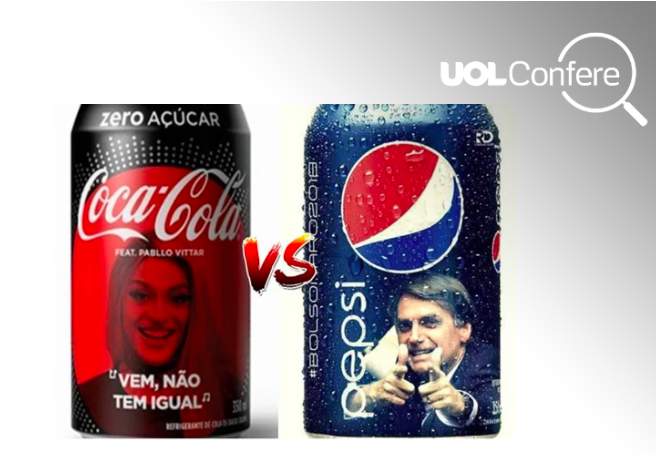
\includegraphics[width=\textwidth]{./imgs/fig3.png}
% \caption{Fonte: Fujita (2017).}
% \end{figure}
% \end{center}

Como podemos perceber, no que depender do atual presidente e de seus
apoiadores, a ``mola progressista'' será cada vez mais reprimida, dadas
as demonstrações de radicalismo ultraconservador lideradas por ele e
reverberadas nas redes sociais de forma orgânica ou com o uso de perfis
falsos e de \textit{bots}. Os chamados robôs sociais ou \textit{social bots} são
contas controladas por \textit{software} que geram artificialmente conteúdo e
estabelecem interações com não robôs. Eles buscam imitar o comportamento
humano e se passar como tal de maneira a interferir em debates
espontâneos e criar discussões forjadas (\textsc{fundação getúlio vargas}, 2017,
p.\,9).

Susskind (2018, p.\,232) afirma que os robôs aprendem por meio de
inteligência artificial a imitar a conversação entre humanos. ``Bots
apenas começaram a colonizar o discurso \textit{online}, mas eles estão
crescendo rapidamente em importância. Um estudo de 2017 estima que 48
milhões (9 a 15\% das contas) no Twitter são bots'' (\textsc{susskind},
2018, p.\,233). O autor alerta que no futuro a forma como percebemos o
mundo será cada vez mais determinada pelo que sistemas digitais nos
revelam ou nos escondem.

\begin{quote}
Esses sistemas --- serviços de notícias e pesquisa, canais de
comunicação, computação afetiva e plataformas de \textsc{ar} --- determinarão o
que sabemos, o que sentimos, o que queremos e o que fazemos. Por sua
vez, aqueles que possuem e operam esses sistemas terão o poder de moldar
nossas preferências políticas. (\textsc{susskind}, 2018, p.\,229)
\end{quote}

Os robôs impulsionam e direcionam o debate político em torno de questões
efêmeras e de micro escândalos criados para desviar a atenção do público
para outras questões sobre as quais os políticos não conseguem ou não
podem debater. Por meio de pautas identitárias, como as relacionadas a
gênero, por exemplo, desvia"-se o foco de outras questões mais urgentes
para as pautas morais, que impactam a opinião pública de forma mais
imediata e expressiva.

Quando o prefeito da segunda maior cidade do país ordena a fiscais da
prefeitura que invadam a Bienal do Livro para recolher uma revista em
quadrinhos com personagens gays, ele está desviando o foco da má gestão
que caracteriza o governo dele, em busca do aumento de popularidade
entre os eleitores mais religiosos. Segundo Gama, Vilicic e Marthe
(2019, p.\,53), a atitude do prefeito foi uma ``clara tentativa de
censura, que inevitavelmente lembra os regimes mais totalitários da
história humana. Segundo os autores, a questão se torna grave quando
crenças religiosas pautam a condução da política.

A permanência de crenças muito arraigadas, quando não há abertura para
visões diferentes, pode fazer com que os efeitos da desinformação
compartilhada de forma efêmera também se tornem permanentes. A mola
antes reprimida pode vir a perder a elasticidade e a flexibilidade que
fazem dela uma mola. É exatamente o que pode acontecer com os fatos em
um mundo contaminado pela desinformação, transformando"-se em um mundo de
verdades rígidas, absolutas e inquestionáveis, ainda que inventadas.
Quase no final de Privacidade Hackeada (em 1 hora e 45 minutos), Carole
apresenta um \textsc{ted}.\footnote{Disponível em \textit{bit.ly/2VYgPx2}.} onde começa falando alguns nomes dos grandes
da tecnologia ``Mark Zuckerberg e Sheryl Sandberg (Facebook), Larry Page
e Sergey Brin (Google), Jack Dorsey (Twitter) vocês se propuseram
conectar pessoas e essa mesma tecnologia está agora nos afastando. E o
que não estão entendendo é que isso é maior do que vocês e é maior do
que qualquer um de nós. E não é sobre direita ou esquerda, ficar ou
largar, ou Trump ou não. É sobre se é realmente possível termos
novamente eleições livres e justas. (\ldots{}) É isso o que querem? É assim
que querem ser lembrados na história? Como servos do autoritarismo?

\begin{bibliohedra}
\tit{alonso}, Ângela. ``A comunidade moral bolsonarista''. \textit{In}: \textsc{abranches}, S. \textit{et al}. \textit{Democracia em risco? 22 ensaios sobre o Brasil hoje}. São
Paulo: Companhia das Letras, 2019.

\tit{bauman}, Zygmunt. \textit{Retropia}. Rio de Janeiro: Zahar, 2019.

\tit{castells}, Manuel. \textit{A sociedade em rede}. vol.\,\textsc{i}. 8ª ed.
revista e ampliada. São Paulo: Paz e Terra, 1999.

\titidem. \textit{Ruptura: a crise da democracia liberal}.
Trad. Joana Angélica d'Avila Melo. Rio de Janeiro: Zahar, 2018.

\tit{ferrari}, Pollyana (org.). \textit{Fluido, fluxo}. Porto Alegre: Fi, 2018.

\titidem. \textit{Como sair das bolhas}. São Paulo: Educ/Armazém da Cultura, 2018.

\tit{fujita}, Gabriela. ``Pepsi vai usar Bolsonaro nas latas após campanha da
Coca com Pabllo Vittar?'' \textit{Uol: Universo Online}, São Paulo, dez. 2017.

\tit{gama}, R.; \textsc{vilicic}, F.; \textsc{marthe}, M. ``Um basta à ignorância''. \textit{Veja}, São Paulo, ed.\,2652, ano 52, n.\,38, set. 2019.

\tit{geli}, Carles. ``Byung"-Chul Han: `Hoje o indivíduo se explora e
acredita que isso é realização'\,''. \textit{El País}, 2018. 

\tit{greenwald}, Glenn. ``Para retratar gays como pedófilos, Carlos Bolsonaro
posta no Twitter cartaz falso há muito desmascarado como fraude''.
\textit{The Intercept Brasil}, Rio de Janeiro, jul. 2018. 


\tit{guattari}, Félix e \textsc{rolnik}, Suely. \textit{Micropolítica: cartografias do desejo.} Rio de Janeiro: Vozes, 1986.

\tit{han}, Byung"-Chul. \textit{Topologia da violência}. Rio de Janeiro: Vozes,
2017.

\titidem. \textit{Bom entretenimento}. Rio de Janeiro: Vozes, 2019.

\tit{linhares}, C.; \textsc{zanini}, F. ``\textsc{mbl} admite culpa por polarização no país e exagero em sua agressividade retórica''. \textit{Folha de S.Paulo}, São
Paulo, jul. 2019.

\tit{mello}, Patrícia. ``Capitalismo esclarecido e populismo de Bolsonaro
aproximarão o Brasil dos \textsc{eua}, diz Steve Bannon''. \textit{Folha de S.Paulo}, São Paulo, out. 2018.

\tit{ortellado}, P. e \textsc{ribeiro}, M. ``Levantamento inédito revela sites e páginas
no Facebook que podem influenciar a eleição com \textit{fake news}''. \textit{Época},
São Paulo, ago. 2018.

\tit{rocha}, Camila. ``O jogo sujo da direita: think tanks ultraliberais e a
nova direita brasileira''. \textit{Le Monde Diplomatique Brasil}, nov. 2017. 

\tit{ruediger}, Marco Aurélio (coord.). \textit{Robôs, redes sociais e política no Brasil: estudo sobre interferências ilegítimas no debate público na web, riscos à democracia
e processo eleitoral de 2018}. Rio de Janeiro, Fundação Getúlio Vargas, 2017.

\tit{susskind}, Jamie. \textit{Future Politics}. Nova York: Oxford University
Press, 2018.
\end{bibliohedra}

\chapterspecial{Ciberpolítica, ciberativismo e cibercultura}{Uma análise dos
\textit{papers} apresentados no grupo de trabalho da \textsc{anpocs}\footnote{Uma
  versão prévia deste artigo foi publicada na Revista Brasileira de
  Informação Bibliográfica em Ciências Sociais (\textsc{bib}), n.\,85 (2018).
  Parte da pesquisa foi realizada com apoio do Laboratório de Análise do
  Campo Científico da Universidade Federal do Paraná (La\textsc{cc}-\textsc{ufpr}).}}{}

\begin{flushright}
\baselineskip=12pt{\textsc{rafael cardoso sampaio}\\
\textsc{isabele mitozo}\\
\textsc{michele goulart massuchin}\\
\textsc{giulia sbaraini fontes}\\
\textsc{cláudio luis de camargo penteado}}
\end{flushright}

\begin{comment}
\textit{Rafael Cardoso Sampaio (\textsc{ufpr})\footnote{Professor adjunto do Curso de Ciências Sociais da Universidade Federal
do Paraná (\textsc{ufpr}). Doutor em Comunicação e Cultura Contemporâneas pela
Universidade Federal da Bahia (\textsc{ufba}). É co"-líder dos grupos de pesquisa
Comunicação e Participação Política (\textsc{compa}) e Laboratório de Análise do
Campo Científico (La\textsc{cc}), ambos sediados na \textsc{ufpr}. Desenvolve pesquisas
sobre democracia digital, governo aberto, campanhas políticas online e
comunicação política.}\\Isabele Mitozo (\textsc{ufpr})\footnote{Pesquisadora em estágio pós"-doutoral no Instituto Nacional de Ciência e
Tecnologia em Democracia Digital (\textsc{inct}.\textsc{dd}), Universidade Federal da
Bahia (\textsc{ufba}). Doutora em Ciência Política pela Universidade Federal do
Paraná (\textsc{ufpr}), tendo realizado estágio de pesquisa na Universidade de
Leeds (Reino Unido). Integrante dos Grupos de Pesquisa em Comunicação,
Internet e Democracia (\textsc{cid}-\textsc{ufba}) e Comunicação, Política e Tecnologia
(\textsc{ponte}-\textsc{ufpr}). Desenvolve pesquisa em democracia digital, parlamentos e
engajamento público, jornalismo e eleições.}\\Michele Goulart
Massuchin (\textsc{ufpr})\footnote{Professora adjunta do Curso de Jornalismo da Universidade Federal do
Maranhão (\textsc{ufma}). Doutora em Ciência Política pela Universidade Federal
de São Carlos (\textsc{ufsc}ar). É pesquisadora associada do Núcleo de Pesquisa
em Comunicação, Política e Opinião Pública (\textsc{cpop}/\textsc{ufpr}) e coordena o
Grupo de Pesquisa em Comunicação, Política e Sociedade (\textsc{cops}/\textsc{ufma}).
Desenvolve pesquisas sobre campanhas eleitorais, jornalismo político e
política e Internet.}\\Giulia Sbaraini Fontes (\textsc{ufpr})\footnote{Doutoranda em Ciência Política da Universidade Federal do Paraná (\textsc{ufpr}).
Mestre em Ciência Política e graduada em Comunicação Social, com
habilitação em Jornalismo, pela mesma instituição. Integrante do Grupo
de Pesquisa Comunicação, Política e Tecnologia (\textsc{ponte}-\textsc{ufpr}). Desenvolve
pesquisas sobre jornalismo político e campanhas eleitorais.}\\Cláudio Luis de Camargo Penteado (\textsc{ufabc})\footnote{Professor associado da \textsc{ufabc}. Doutor em Ciências Sociais pela \textsc{puc} \textsc{sp}.
Pesquisador do Laboratório de Tecnologias Livres da \textsc{ufabc} e do Núcleo de
Estudos em Arte, Mídia e Política da \textsc{puc} \textsc{sp}. Desenvolve pesquisas sobre
Internet e Políticas públicas, debate político nas redes sociais e
cibercampanhas.}}
\end{comment}

\noindent{}A Internet nasce do improvável encontro entre o projeto militar de
comunicação (\textsc{arpanet}), da inserção da \textit{big science} no
desenvolvimento de tecnologias de informação e da cultura libertária
californiana (\textsc{castells}, 2003). Segundo o sociólogo catalão, a junção
desses três movimentos, com perfis diferenciados, criou condições
econômicas, tecnológicas e culturais para a formação de uma nova
estrutura comunicacional com o uso de microprocessadores e estruturada
na forma de rede distribuída, que vem provocando profundas
transformações sociais, econômicas, políticas e culturais. Por sua vez,
a Internet comercial surge em meados dos anos 80, enquanto a \textit{world
wide web} é de meados dos anos 90 e rapidamente se torna a tecnologia de
comunicação e informação (\textsc{tic}) com a mais rápida expansão da história
humana.\footnote{Em 2001, 8\% da população mundial tinha acesso à rede
  mundial de computadores, enquanto já são 45,9\% da população em 2016,
  segundo os dados do \textit{Telecommunication Development Sector}
  (\textsc{itu}--D). No Brasil, o número de usuários já passa da metade da
  população, atingindo 58\% dos cidadãos e representando 102 milhões de
  internautas (\textsc{cgi}.br).}

Mesmo que ainda exista uma grande parcela da população mundial sem
acesso à Internet, os efeitos e as transformações do uso dessa
tecnologia já se impõem diretamente para quase toda a população mundial,
mesmo que de forma indireta. A arquitetura distribuída, o
desenvolvimento de processos colaborativos e a interatividade entre os
usuários possibilitam a emergência de novas relações tecidas de forma
horizontal nesse meio. Nesse sentido, emerge um novo modelo de
reestruturação da produção, organizado em rede e de acordo com o uso
crescente das \textsc{tic}s, em que a informação assume o papel de matéria"-prima
na constituição da sociedade em rede (\textsc{castells}, 1999).

Nesse contexto, boa parte das questões iniciais sobre essa aproximação,
do ponto de vista político, se deram na perspectiva de responder o que a
Internet pode fazer pela democracia, recebendo tanto respostas bastante
céticas quanto entusiasmadas sobre os potenciais dos, então, novos meios
de comunicação e informação. O efeito das tecnologias eletrônicas e
digitais sobre as atividades políticas, sociais e culturais se configura
como preocupação relativamente antiga nas ciências humanas e sociais.

Conforme estudo realizado por Gomes (2016), a atenção acadêmica sobre as
relações existentes entre os meios digitais e as práticas políticas já é
consolidada, havendo mais de quatro mil estudos em quase 25 anos de
existência, com o estabelecimento de, ao menos três grandes áreas de
estudo: e"-política, democracia digital e Estado digital, com as práticas
sociais ganhando proeminência no primeiro eixo.

Em relação ao Brasil, o estudo de Sampaio, Bragatto e Nicolás (2016)
analisa 526 artigos publicados nos principais eventos acadêmicos de
Comunicação e de Ciências Sociais no país, no período de 2000 a 2014,
demonstrando que aquelas subáreas estão também consolidadas na pesquisa
nacional. Por outro lado, há uma concentração de artigos apresentados em
eventos de Comunicação e também por pesquisadores desta área
(45,6\%), enquanto pesquisadores dos programas de pós"-graduação das
áreas de ciências sociais em conjunto (ciências sociais, ciência
política, sociologia) representam 29,4\% da população. Dessa maneira,
considerando a consolidação do \textsc{gt} Ciberpolitica, ciberativismo e
cibercultura na \textsc{anpocs} --- criado em 2010 e mantido de forma ininterrupta
até então --- , é nosso objetivo investigar, exclusivamente, os trabalhos
apresentados neste espaço, compreendendo"-o como uma pequena amostra do
interesse e relevância acadêmica das ciências sociais pelo tema.

Desse modo, o artigo se divide em cinco seções. A primeira delas
apresenta um panorama da consolidação das pesquisas em cibercultura e
ciberpolítica no país, dando destaque para a criação de grupos de
trabalho (\textsc{gt}s) em eventos acadêmicos de comunicação e de ciências
sociais e para a consolidação do campo de pesquisa. Mais adiante,
apresentam"-se os procedimentos metodológicos adotados pela pesquisa. A
terceira seção consiste na análise dos dados obtidos, que é seguida da
discussão dos resultados. Por fim, apresentam"-se algumas considerações
finais sobre a investigação, abrindo espaços a pesquisas mais
abrangentes sobre a incidência dos trabalhos acerca da temática em tela
em outros eventos nacionais.

\section{Internet, Política e Cibercultura: a consolidação de uma nova área de pesquisa}

A área de pesquisa de ciberpolítica, ciberativismo e cibercultura se
caracteriza pela interdisciplinaridade e pelas constantes inovações
tecnológicas que refletem sobre a dinâmica do objeto e dos métodos de
pesquisa. Situada em zonas de fronteira entre a Comunicação e as
Ciências Sociais, com aportes e diálogos com outras áreas do
conhecimento (administração, ciência da informação, ciência da
computação, direito, filosofia, psicologia etc.), cria"-se uma área
aberta para contribuições de saberes provenientes de diferentes áreas.
As rápidas transformações das \textsc{tic}s levam ao surgimento de novas agendas
que visam estudar as mudanças inseridas pelas inovações tecnológicas,
desafiando pesquisadores e pesquisadoras com novos problemas de
pesquisa, assim como novas técnicas para a investigação científica.

Os primeiros estudos acadêmicos voltados para a área ocorrem no campo da
Cibercultura, no qual pesquisadores, geralmente de Comunicação,
começam a estudar a emergência de novas práticas culturais que se
estabelecem pelo uso e pela interação com as tecnologias de informação e
comunicação (\textsc{ntic}). Segundo Amaral e Montardo (2012), o termo
\textit{cibercultura} é popularizado entre a metade dos anos 80 e início dos anos
90 e chega ao Brasil em torno de 1996 em textos de André Lemos e Eugênio
Trivinho. A título de exemplo, a tradução do influente livro
\textit{Cibercultura}, de Pierre Lévy, seria lançada em 1999 no Brasil,
enquanto André Lemos lançaria o livro \textit{Cibercultura: tecnologia e
vida social na cultura contemporânea} em 2002, marcando em definitivo
tal área de estudos no Brasil (\textsc{lemos}, 2002).

Segundo Lévy (1999, p.\,17), ``cibercultura especifica o conjunto de
técnicas (materiais e intelectuais), de práticas, de atitudes, de modos
de pensamento e de valores que se desenvolvem juntamente com o
crescimento do ciberespaço''. Ou seja, análises e reflexões acerca dos
impactos das tecnologias digitais e móveis em ``hábitos sociais,
práticas de consumo cultural, ritmos de produção e distribuição da
informação, {[}criam{]} novas formas de sociabilidade de comunicação
social'' (\textsc{lemos \& lévy}, 2010, p.\,22).

Para Lemos e Lévy (2010), a cibercultura estaria assentada em três
princípios fundamentais. O tripé seria composto de 

\begin{enumerate}
\item Liberação do pólo de emissão ou da palavra, ou seja, as múltiplas possibilidades geradas pelos meios digitais para as pessoas passarem a emitir suas próprias informações ao invés de apenas serem expectadores das mídias massivas, o que impactaria na emergência de novas formas de comunicação e de veiculação da opinião pública;

\item Princípio da inteligência coletiva, segundo o qual a interconexão planetária aliada à liberação da emissão permitiria o estabelecimento de sinergia entre competências, recursos e projetos que envolvessem a ativação de modos de cooperação flexíveis e transversais, permitindo a criação de um conhecimento coletivo que não seria possível ser alcançado individualmente; sendo que os dois princípios acima impactam em:

\item Reconfiguração social, cultural e política, que é baseada em funções pós"-massivas da comunicação. O ``sistema pós"-massivo permite a personalização, o debate não mediado, a conversação livre, a desterritorialização planetária'' (\textsc{lemos \& lévy}, 2010, p.\,26). 
\end{enumerate}

Na área de Comunicação, a cibercultura seria institucionalizada com a
criação de grupos de trabalho (\textsc{gt}s) específicos nos principais eventos
da área, nomeadamente Intercom e Compós, e com a criação de linhas de
pesquisa em programas de pós"-graduação, como foi o caso do \textsc{ppgcom} da
Universidade Federal da Bahia. Houve, ainda, a publicação da coletânea
\textit{Cibercultura} pela editora Sulina, que passou a publicar coletâneas e
livros autorais sobre o tema, incluindo as duas obras citadas mais acima
(\textsc{amaral \& montardo}, 2012). A institucionalização culminaria na criação,
em 2006, da Associação Brasileira de Pesquisadores em Cibercultura
(\textsc{abc}iber), que passou a realizar eventos anualmente em uma série de
temáticas existentes dentro do assunto, incluindo diversas delas
próximas aos objetos da interface \textit{Internet e política}. Até 2017, dez
encontros anuais haviam sido realizados.

Como uma área bastante abrangente de estudos, a cibercultura realizou
parte das primeiras reflexões acerca dos impactos dos novos meios sobre
cultura, sociabilidade e política, fazendo pesquisas sobre as inovações
tecnológicas e suas apropriações por cidadãos usuários. Foram
estabelecidas, assim, intersecções não apenas com outras áreas da
Comunicação, como o jornalismo (\textit{i.\,e.} ciberjornalismo), mas também com as
ciências sociais, como foi o caso das reflexões acerca do impacto do
digital sobre formas de ação coletiva (\textit{i.\,e.} ciberativismo) ou mesmo
sobre técnicas de pesquisa da Antropologia, por exemplo a \textit{netnografia}.

Paralelamente a isso, podemos falar da subárea da \textit{Internet e política} 
ou ciberpolítica. Diferentemente do campo da cibercultura,
ela surgiria como um subcampo de estudos de comunicação e política e,
consequentemente, como uma área interdisciplinar entre a comunicação
social e a ciência política. Segundo Miguel e Biroli (2010), o interesse
nas relações entre mídia e política estaria centrado em quatro pontos:
na mídia que se tornou o principal instrumento de contato entre a elite
política e os cidadãos comuns; na mídia que é a principal responsável pela
produção da agenda pública, o que levou; no discurso político a
transformar"-se, adaptando"-se às formas preferidas pelos meios de
comunicação de massa; e, por fim, nos candidatos a posições de destaque político que
têm de adotar uma preocupação central com a gestão de suas visibilidades
e imagens públicas (\textsc{gomes}, 2004; \textsc{weber}, 2009).

Para diversos pesquisadores, esta mudança apontava para uma certa
substituição dos partidos políticos pelos meios de comunicação de massa
como intermediadores entre cidadãos e políticos, em situações tais como:
definir a agenda dos temas relevantes para a discussão na esfera
pública; gerar e transmitir informações políticas; fiscalizar a
ação das administrações públicas; exercer a crítica das políticas
públicas e canalizar as demandas da população junto ao governo (\textsc{lima},
2009).

Como indicado por Rubim e Azevedo (1998), os estudos sobre comunicação e
política já existem desde a década de 70 e 80 no Brasil (ainda sobre a
alcunha \textit{comunicação e poder}), ``articulados pela preocupação
dominante de pensar as mídias como aparelhos de luta política e
principalmente ideológica'' (p.\,190). A área, entretanto, ganha
verdadeiramente força após o processo de redemocratização com as
eleições presidenciais de 1989.

Alguns outros fatores são importantes para a compreensão da consolidação
da pesquisa acerca da comunicação e política. Como ressaltado por Lima
(2009), ``as características históricas específicas do sistema de mídia
no Brasil potencializam o seu poder no processo político'' (p.\,28), como
a falta de regularização no setor, o que permitiu oligopólios,
propriedades cruzadas e forte alinhamento de famílias e setores
midiáticos com governantes no período da Ditadura Militar, como foi o
caso das organizações Globo. Isso é reforçado pelas ``características
específicas da população brasileira {[}que{]} historicamente
potencializaram o poder da mídia no processo político, sobretudo, no
processo eleitoral'' (p.\,29), como o alto analfabetismo, a baixa
escolarização e o baixo interesse político. Finalmente, a implantação do
inovador modelo do Horário Gratuito de Propaganda Eleitoral (\textsc{hgpe}) pode
ser considerado um último marco desse momento inicial. Sendo de exibição
obrigatória nos sistemas de rádio e \textsc{tv}, o \textsc{hgpe} é um espaço exclusivo aos
agentes políticos e suas campanhas e com significativos efeitos sobre
elas e as intenções de voto (ao ponto de influenciar a união de
coligações pelo ``tempo de \textsc{tv}''). Ele se tornaria rapidamente um dos
objetos mais estudados pela área de comunicação e política (\textsc{albuquerque},
2010; \textsc{dias}, 2013; \textsc{figueiredo} \textit{et al.}, 1997; \textsc{panke \& cervi}, 2011).
Segundo Marcus Figueiredo, a eminência do \textsc{hgpe} nas campanhas eleitorais
teria sido um importante marco para o crescente interesse da ciência
política na temática.

Conforme a pesquisa de Sampaio, Bragatto e Nicolás (2016, p.\,288), os
estudos sobre \textsc{i\&p} ou ciberpolítica começam a surgir
logo após os anos 2000, fazendo reflexões mais gerais acerca da
regulação do novo meio e o~impacto da Internet sobre instâncias
políticas tradicionais, como ``engajamento cívico, formação da vontade
política, criação ou reforço da coesão social entre grupos de interesse,
participação política, capital social, cultura política, relação entre a
classe dos representantes e dos representados, campanhas políticas''.
Segundo os autores, apesar de ser uma subárea dentro de outra (ou seja,
ela nasce dentro de interesses mais ampliados de comunicação e
política), a ciberpolítica teria características próprias e diferentes
da área maior, notadamente associada às especificidades tecnológicas.

Enquanto as relações sobre mídia e política são constantemente avaliadas
sob um viés negativo que denota o esvaziamento do discurso político para
se adaptar à gramática midiática e à geração de uma espiral do cinismo
fomentada pela cobertura constantemente negativa das ações políticas
pelo jornalismo (\textsc{gomes}, 2004), a ciberpolítica teria, originalmente, uma
visão mais otimista sobre o potencial dos (então) novos meios para a
mitigação de \textit{déficits} democráticos. Isso pode ser constatado
empiricamente pela análise realizada por Sampaio \textit{et al.} (2016),
que denota a importância de temas da democracia digital (participação,
deliberação e engajamento) sobre temas da política digital, como
estratégia política e campanhas eleitorais. Para Gomes (2016), na
verdade, todos os estudos sobre \textsc{i\&p} são em maior ou
menor medida gestados originalmente sob o guarda"-chuva intelectual da
democracia digital. Em um primeiro momento, era necessária a
justificativa de recursos e esforço acadêmico para os novos meios, o que
foi alcançado pela legitimidade trazida por estudos pensados em gestar
melhorias para a democracia. Não obstante, os estudos mais empíricos e
mais orientados a outras questões, que não democráticas, passam
gradativamente a ganhar força e espaço, seja no caso internacional
(\textsc{gomes}, 2016), seja no brasileiro (\textsc{sampaio} \textit{et al.}, 2016).

Cabe destacar também os estudos sobre o ativismo \textit{online},
\textit{webativismo} ou \textit{ciberativismo}. As pesquisas dessa subárea
nascem das iniciativas pioneiras do uso das \textsc{tic}s pelo movimento
Zapatista no México e dos movimentos antiglobalização no final do
século. Outros campos de investigação estão voltados para os estudos
sobre as ações de \textit{hacktivismo} em favor da emancipação social pelo
acesso às informações (\textsc{silveira}, 2010); o uso dos dispositivos da
Internet pelas organizações da sociedade civil na influência de
políticas públicas (\textsc{araújo} \textit{et al.}, 2015); e para as
mobilizações políticas pelo uso de mídias sociais para expressão de
indignação e esperança --- que tiveram início com o ciclo de protestos
conhecidos como a Primavera Árabe e se espalharam por diversas regiões
do planeta, chegando no Brasil em junho de 2013 (\textsc{castells}, 2017). Com o
avanço das \textsc{tic}s, diversos grupos e organizações ativistas incorporam o
uso dos dispositivos de comunicação da Internet em suas práticas de
mobilização e divulgação de informações, de forma que hoje já não existe
mais a distinção entre ativismo \textit{online} e \textit{offline} (\textsc{harlow
\& harp}, 2012).

Em termos acadêmicos, no Brasil, é preciso apontar o papel pioneiro do
\textsc{gt} Comunicação e Política, já presente na criação dos \textsc{gt}s da
Associação Nacional dos Programas de Pós"-Graduação em Comunicação
(\textsc{compós}) em 1992, por iniciativa de pesquisadores diversos da interface,
como Antônio Albino Canelas Rubim, Maria Cerés Pimenta, Maria Helena
Weber, Murilo Ramos, Sergio Porto, Wilson Gomes, entre outros.
Posteriormente, a primeira institucionalização por parte da ciência
política ocorre em 1997 com a criação do \textsc{gt} Mídia, opinião pública e
eleições na Associação Nacional de Pós"-Graduação e Pesquisa em
Ciências Sociais (\textsc{anpocs}), por intermédio dos professores Marcus
Figueiredo (\textsc{iuperj}) e Vera Chaia (\textsc{puc~--~sp}).

Por sua vez, a criação da Associação dos Pesquisadores em Comunicação e
Política (Compolítica), em 2006, é um marco na consolidação da área
interdisciplinar entre Comunicação e Ciência Política, uma vez que esse
passa a ser o primeiro evento exclusivamente voltado às diferentes
temáticas existentes do campo. Em especial, a Compolítica apresenta o
primeiro \textsc{gt} \textit{stricto sensu} a levar a alcunha Internet e
Política, coordenado pelo professor Wilson Gomes. No caso da Ciência
Política, a linha de Comunicação e Política consolidava sua presença com
a criação da área temática ``Comunicação política e opinião pública'' no
congresso da Associação Brasileira de Ciência Política (\textsc{abcp}) de 2008,
por Alessandra Aldé (\textsc{uerj}) e Marcus Figueiredo (\textsc{iuperj}), o que se mantém
até os dias atuais.

A rápida difusão das \textsc{tic}s na sociedade e seu uso massivo por diversos
atores e segmentos sociais gerou uma demanda específica de estudos
acerca dos impactos e dos efeitos das tecnologias digitais na sociedade,
na cultura e no sistema político formal e informal. A emergência desse
campo de estudos envolve questões e abordagens de diferentes áreas de
conhecimento, composto de uma agenda de pesquisa dinâmica e
interdisciplinar, que a cada dia atrai mais pesquisadores (de diferentes
áreas do saber), interessados em estudar os efeitos e transformações
sociais, culturais, tecnológicas e políticas.

Advinda de maneira mais direta da discussão sobre comunicação e
política, no geral, e da \textsc{i\&p}, em específico, mas com uma
preocupação especial em ofertar um novo espaço para outras discussões
possíveis a respeito do tema, é criado, em 2010, o \textsc{gt} Ciberpolítica,
Ciberativismo e Cibercultura, coordenado pelos professores Sérgio
Amadeu da Silveira, da \textsc{ufabc}, e Sérgio Braga, da \textsc{ufpr}, grupo que se
mantém regularmente ativo até a apresentação deste estudo. A
consolidação do \textsc{gt} permite identificar que existe um campo de estudo
específico de pesquisas com foco em Internet nas ciências sociais
contemporâneas, com objetos, temáticas e métodos específicos, que
interage com outras áreas de estudo, criando uma diversidade de
pesquisas e reflexões sobre a influência e o impacto das \textsc{tic}s na
sociedade contemporânea, assim como o estudo de novas práticas que se
estabelecem pelo uso crescente das tecnologias digitais.

A seção seguinte procura apresentar de modo detalhado os procedimentos
adotados pela investigação, que possui caráter exploratório, não
partindo, portanto, de hipóteses acerca dos dados obtidos, sobretudo
porque o \textit{corpus} é composto de textos de apenas um Grupo de
Trabalho que acolhe a área, dentre tantos \textsc{gt}s em outros eventos de
âmbito nacional, atualmente.

\section{Procedimentos Metodológicos}

A primeira etapa dessa pesquisa consistiu na coleta dos textos que
formariam o \textit{corpus} do \textit{paper}. Esse processo foi realizado a
partir do \textit{website} da \textsc{anpocs}, onde estão armazenados os trabalhos de todas as edições do encontro
anual. A partir dessa consulta, foram reunidos 106
\textit{papers} apresentados no \textsc{gt} Ciberpolítica, Ciberativismo e
Cibercultura entre 2010, ano em que o grupo de trabalho foi criado, e
2017. Foram consideradas tanto apresentações orais quanto painéis, já
que não há essa distinção no site da Associação. Na primeira tabela, abaixo,
apresentamos a distribuição dos trabalhos nos anos contemplados pela
pesquisa. As variações no número de artigos disponibilizados ocorrem
porque, mesmo que exista uma margem fixa de textos aceitos pelo \textsc{gt} (em
torno de doze apresentações orais e cinco painéis), nem todos os
autores disponibilizam a versão completa após o evento.
\enlargethispage{\baselineskip}


\begin{figure}[!ht]
%\resizebox{\textwidth}{!}{
\begin{center}
\begin{tabular}{|c|c|c|}
\hline
\textsc{ano} & \textsc{frequência} & \textsc{\%} \\ \hline\hline
2010 & 15 & 14,2\% \\ \hline
2011 & 14 & 13,2\% \\ \hline
2012 & 16 & 17\% \\ \hline
2013 & 10 & 9\% \\ \hline
2014 & 13 & 12,3\% \\ \hline
2015 & 10 & 9,4\% \\ \hline
2016 & 14 & 13,2\% \\ \hline
2017 & 14 & 13,2\% \\ \hline
\textbf{Total} & \textbf{106} & \textbf{100}\% \\ \hline
\end{tabular}
\end{center}
\caption{Distribuição dos artigos por ano.\footnotemark}

\end{figure}

\footnotetext{Fonte: Elaboração própria, 2017.}

Após a coleta do \textit{corpus}, foi realizada uma Análise de Conteúdo
quantitativa. O livro de códigos construído para a pesquisa toma por
base o artigo de Sampaio, Bragatto e Nicolás (2016), adaptando algumas
categorias das variáveis de acordo com nosso objeto de estudo.\footnote{Em
  caso de interesse em replicar e/\,ou ampliar o estudo, entrar em contato
  com os autores por e"-mail para a disponibilização do livro de códigos
  ou mesmo do banco de dados.} As 17 variáveis analisadas
dividem"-se em dois grupos: aquelas que se referem a autores e outras
que dizem respeito à pesquisa apresentada.

Em relação às características dos autores, as variáveis foram: quantidade de autores; sexo; instituição; escolaridade; área de escolaridade; parceria institucional; parceria interdisciplinar. 
Em relação às características dos trabalhos, as variáveis foram: área temática do artigo; vertente; objeto político/social; objeto tecnológico; abordagem teórica; tipo de estudo; tipo de método; tipo de técnica; aplicação (ou não) de estatística; e qual tipo de estatística.

No primeiro grupo, de variáveis que se referem às características dos
autores, foram levantadas informações como sexo, instituição à qual
pertence, grau de escolaridade e área em que o pesquisador atua.
Além disso, nos casos em que havia mais de um autor, observou"-se se
eles pertenciam a diferentes instituições de ensino (parceria
institucional) e/\,ou a distintas áreas de pesquisa (parceria
interdisciplinar).

Após esse primeiro levantamento, os codificadores passaram à análise do
conteúdo dos textos. Inicialmente, os trabalhos foram classificados de
acordo com a área temática a que pertenciam: ciberpolítica,
ciberativismo ou cibercultura. Os \textit{papers} foram considerados 
de vertente social, quando diziam respeito a engajamento cívico, por
exemplo; ou de vertente institucional, quando se relacionavam a
iniciativas de interação entre Estado e cidadãos.\footnote{Conforme a
  pesquisa de Sampaio e colegas (2016, p.\,295), na vertente social,
  ``estariam as implicações do meio no engajamento cívico, na esfera
  pública, na deliberação política e na sua relação com o capital
  social. Em comum, a preocupação com a formação e as aptidões políticas
  da cidadania no ciberespaço.''}. Segundo Gomes, a vertente
  institucional teria três endereços: 

\begin{enumerate}
\item  A conformação digital das instituições da democracia em sentido estrito (cidades e governos digitais, parlamentos \textit{online}) ou lato (partidos políticos \textit{online});

\item As iniciativas institucionais no vetor que vai do Estado aos cidadãos, como a prestação de serviços públicos \textit{online} e governo eletrônico;

\item Iniciativas institucionais no vetor cidadãos"-Estado: oportunidades de participação ou de oferta de inputs por parte da cidadania na forma de votos, respostas a sondagens, decisões ou sugestões orçamentárias, registro e discussão de opiniões em fóruns eletrônicos etc. (\textsc{gomes}, 2007, p.\,11).
\end{enumerate}

Depois dessa primeira classificação ampla, observou"-se qual era o objeto
político ou social explorado no artigo. Além disso, os trabalhos foram
classificados de acordo com o objeto tecnológico que exploravam. Outro
aspecto verificado na análise diz respeito à abordagem teórica
predominante nos textos.

Na variável \textit{tipo de estudo} os \textit{papers} foram classificados como
teóricos ou empíricos. Em seguida, ao considerar o método utilizado na
pesquisa, os trabalhos poderiam ser quantitativos, qualitativos,
bibliográficos ou quantitativos e qualitativos, simultaneamente. Estudos
teóricos, nesse caso, foram sempre classificados como bibliográficos.
Somente para estudos empíricos, por fim, foram analisadas outras três
variáveis. No caso de estudos empíricos, foi verificada a técnica de
pesquisa aplicada e se houve o uso de técnicas estatísticas.

Esse livro de códigos foi aplicado aos 106 trabalhos do \textit{corpus}
por três codificadores, após um treinamento para que houvesse
concordância entre eles. A partir disso, a fim de apreender outras
características dos artigos analisados, a pesquisa lança mão de técnicas
estatísticas para auxiliar na análise e no cruzamento dos dados, como o
uso de frequências simples, cálculo de qui"-quadrado e análise de
resíduos padronizados. Os resultados são, então, apresentados no tópico
a seguir.

\section{o \textsc{gt} Ciberpolítica, Ciberativismo e
Cibercultura}

\subsection{Características dos autores}

A partir da análise dos textos que constituem o \textit{corpus} empírico
(\textsc{n}\,=\,106), é possível chegar a alguns achados importantes sobre o modo
como o referido \textsc{gt} se estruturou ao longo dos anos, mapeando e inserindo
vertentes de pesquisa e instituições. Pode"-se, primeiramente, depreender
que, mesmo que a maior parcela dos \textit{papers} se concentre na
parceria entre dois ou mais autores (que somados chegam a 58,5\%), há
predomínio exclusivo da categoria \textit{autoria individual} nos trabalhos
apresentados no \textsc{gt}, conforme pode ser visto na tabela abaixo. Dentre
eles, 41,5\% são de apenas um autor. Além disso, é possível dizer
que esta constatação inicial já diminui, de forma significativa, a
possibilidade de pesquisas interinstitucionais, o que vai ser analisado
adiante.

Em relação ao número de autores, dos 106 \textit{paper} analisados, 44 tinham apenas um autor (41,5\%); 27 tinham dois autores (25,5\%); 31 tinham três autores (29,2\%); e quatro tinham quatro autores (3,8\%).

\begin{comment}
\begin{center}
Tabela 2: Número de autores por \textit{paper} apresentado
\end{center}

\begin{center}
\centering
\begin{tabular}{|l|l|l|}
\hline
 & Frequência & Percentual \\ \hline
1 & 44 & 41,5 \\ \hline
2 & 27 & 25,5 \\ \hline
3 & 31 & 29,2 \\ \hline
4 & 4 & 3,8 \\ \hline
Total & 106 & 100 \\ \hline
\end{tabular}
\end{center}

\begin{center}
{\footnotesize\textit{Fonte: Elaboração própria, 2017.}}
\end{center}
\end{comment}

Outra variável analisada é o sexo dos autores. Neste caso, são
agregados os dados dos três primeiros autores, que foram
computados na codificação. O objetivo é identificar se há pluralidade no
Grupo de Trabalho. Percebe"-se que, embora haja equilíbrio na autoria
principal, com 53 mulheres como primeiras autoras e 53 homens na mesma
categoria, no total ainda há mais homens participando do \textsc{gt}, em todas as
outras posições de autoria observadas. Normalmente, quando há a inclusão
de mais de um autor, estes tendem a ser homens e não mulheres, o que
acaba desequilibrando o total: com dois autores, 24 são mulheres e 38 homens; com três, 13 são mulheres e 22 são homens; com quatro, 90 são mulheres e 113 são homens.\footnote{Temos os dados de 203 e não de 207 autores, pois apenas quatro dos 106 trabalhos possuem quatro autores e na pesquisa faz"-se a coleta dos dados referentes aos três primeiros, uma vez que aquele total foi mínimo. Ressalta"-se que em 2017 houve uma restrição de cadastro para os alunos de graduação.} O conjunto dos presentes no \textsc{gt} ao longo
dos anos foi composto de 44,3\% de mulheres e 55,7\% de homens.

\begin{comment}
\begin{center}
Tabela 3: Sexo dos autores e autoras dos trabalhos
\end{center}

\begin{center}
\centering
\begin{tabular}{|l|l|l|l|l|l|}
\hline
Sexo & 1º & 2º & 3º & 4º & \% Total \\ \hline
Mulher & 53 & 24 & 13 & 90 & 44,3 \\ \hline
Homem & 53 & 38 & 22 & 113 & 55,7 \\ \hline
Total & 106 & 62 & 35 & 203\footnotemark & 100 \\ \hline
\end{tabular}
\end{center}

\begin{center}
{\footnotesize\textit{Fonte: Elaboração própria, 2017.}}
\end{center}

\footnotetext{Temos os dados de 203 e não de 207 autores, pois apenas quatro dos 106 trabalhos possuem quatro autores e na pesquisa faz-se a coleta dos dados referentes aos três primeiros, uma vez que aquele total foi mínimo. Ressalta-se que em 2017 houve uma restrição de cadastro para os alunos de graduação.}
\end{comment}

É importante saber, ainda, se há rotatividade desses pesquisadores
durante os oito anos e se há aqueles que se repetem com frequência,
ou seja, que participaram várias vezes do evento. O primeiro dado indica
que, entre os 203 autores, há certa repetição ao longo do tempo.
Logo, no total, há 130 autores únicos. 


\begin{comment}
A tabela seguinte permite identificar a rotatividade do \textsc{gt}.

\pagebreak
\begin{center}
Tabela 4: Rotatividade de autores no \textsc{gt}
\end{center}

\begin{center}
\centering
\begin{tabular}{|l|l|l|}
\hline
\textbf{Repetição} & \textbf{Quantidade} & \textbf{Percentual} \\ \hline
1 & 96 & 73,8 \\ \hline
2 & 18 & 13,8 \\ \hline
3 & 9 & 6,9 \\ \hline
4 & 2 & 1,5 \\ \hline
5 & 0 & 0 \\ \hline
6 & 1 & 0,8 \\ \hline
7 & 2 & 1,5 \\ \hline
8 & 2 & 1,5 \\ \hline
Total & 130 & 100 \\ \hline
\end{tabular}
\end{center}

\begin{center}
{\footnotesize\textit{Fonte: Elaboração própria, 2017.}}
\end{center}
\end{comment}

Em relação à rotatividade do \textsc{gt}, constatamos que
96 autores (73,8\% do total) participaram
apenas uma vez ao longo dos oito anos. Outros 18 participaram de duas
edições, o que equivale a outros 13,8\%. Nove participaram três vezes (6,9\%), dois participaram quatro vezes (1,5\%), um participou seis vezes (0,8\%), dois participaram sete vezes (1,5\%), mesmo número para os que participaram em oito edições (1,5\%).
Logo, pode"-se perceber que em
cada edição do evento não há tendência à repetição de autores. Do
total de 130 autores, 16 deles participaram de três edições ou
mais.

É importante notar que, dentre os cinco autores que mais se
repetiram ao longo do \textsc{gt} (em 8, 7 ou 6 edições), há apenas uma mulher.
Ainda discutindo gênero, verifica"-se que os homens são quase sempre
maioria nas sessões, como segue no gráfico abaixo, quando se observa a
distribuição longitudinal.


 \begin{figure}[!ht]
 \centering
  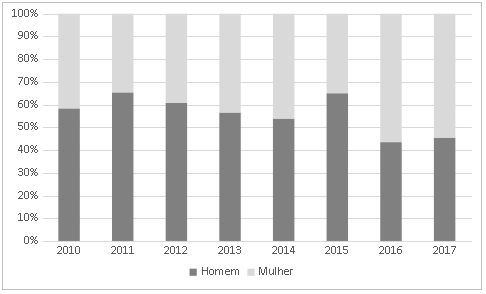
\includegraphics[width=70mm]{./imgs/graf3_1.png}
 \caption{Distribuição de homens e mulheres ao longo dos anos no \textsc{gt}\footnotemark}
 \end{figure}
 
 \footnotetext{Fonte: Elaboração dos autores, 2017.}

Apenas em 2016 e 2017 houve maior presença de mulheres (57\% e 55\%,
respectivamente) do que homens no referido grupo de trabalho. As maiores
diferenças estão em 2011 e 2015, com mais de 65\% dos participantes
homens. Dessa forma, não há um crescimento contínuo da paridade, que
ocorre de modo mais próximo em 2013, 2014 e 2017. Assim, apesar da
repentina visibilidade das mulheres em 2016, elas são, no total,
minoria.

Outra variável observada pela pesquisa é a universidade representada
pelos autores. Os dados também são agregados e se referem aos
três autores do \textit{paper} apresentado. Conforme os dados abaixo,
há uma concentração da representação de quatro universidades, que
aparecem em quase todos os anos e são centros de referência em estudos
da área.



 \begin{figure}[!ht]
 \centering
  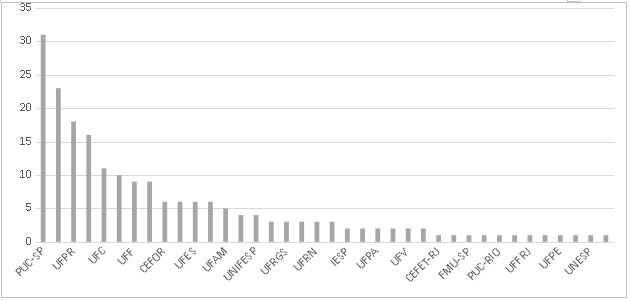
\includegraphics[width=\textwidth]{./imgs/graf3_2.png}
 \caption{Distribuição das universidades dos autores\footnotemark}
 \end{figure}
 
 \footnotetext{Fonte: Elaboração dos autores, 2017.}

A \textsc{puc} de São Paulo, a \textsc{ufabc}, a \textsc{ufpr} e a \textsc{ufmg} reúnem 42\% de todos os
autores que já participaram do \textsc{gt}. Houve, ademais, um único autor de
instituição estrangeira, da Universidade da Beira Interior (\textsc{ubi}, de Portugal). A região Norte aparece representada por \textsc{ufam}, Unama, \textsc{ufpa} e
\textsc{ifto}, com cinco autores para o caso da \textsc{ufam} e uma autora cada para as
demais, respectivamente, durante o período. O Nordeste aparece
representado por \textsc{ufba}, \textsc{ufpb}, \textsc{ufrn}, \textsc{ufpe}, \textsc{ufc}, mas em pouca quantidade em
relação ao predomínio das universidades que lideram. Inclusive, chama a
atenção a pouca presença de trabalhos da \textsc{ufba}, que atualmente é a
instituição sede do Instituto Nacional de Ciência e Tecnologia sobre
Democracia Digital (\textsc{inct}.\textsc{dd}) e do Laboratório de Pesquisa em Mídia
Digital, Redes e Espaço (Lab 404),\footnote{Dedicado a estudos sobre
  Cibercultura.} cujas pesquisas entrariam no escopo do \textsc{gt} em
tela.

Destaca"-se que as universidades mais representadas, como \textsc{puc~--~sp}, \textsc{ufabc}, \textsc{ufpr}
e \textsc{ufmg}, estão nas regiões Sul e Sudeste apenas. Das 38 que apareceram,
22 são da região Sudeste. Ademais, há três do Sul, quatro do Norte, três
do Centro"-Oeste e cinco do Nordeste. Além da observação das
instituições, há dados sobre a escolaridade dos autores. Da mesma
forma, estão agregados os números relacionados aos três autores
(203 casos).\footnote{Trabalhamos com a autoria de todos os
  \textit{papers}, logo, contabilizam"-se as autorias de cada trabalho, não
  os autores em si, como outrora neste trabalho, que no total são 130
  \textit{autores únicos}.}



 \begin{figure}[!ht]
 \centering
  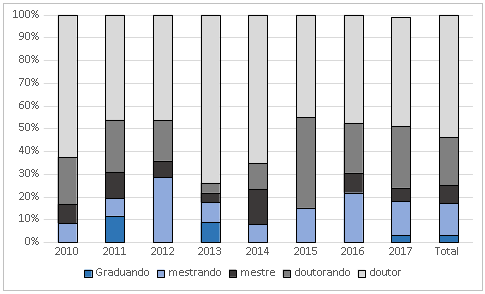
\includegraphics[width=90mm]{./imgs/graf3_3.png}
 \caption{Distribuição da escolaridade de autores durante os oito anos\footnotemark}
 \end{figure}
 
\footnotetext{Fonte: Elaboração dos autores, 2017.}

Percebe"-se, a partir da leitura da última coluna do gráfico, que grande
parte dos primeiros autores de \textit{papers} é composta de
doutores (54\%), seguidos de longe por doutorandos (21\%). A
baixa incidência de mestres pode apontar para o fato de que o evento
é almejado por quem está ativamente no meio acadêmico, seja como docente
ou discente de programas de pós"-graduação. Com relação aos
mestrandos (14\%), a frequência mais próxima àquela de doutorandos
pode indicar maior ocorrência de trabalhos desses estudantes na
modalidade painel, que não é diferenciada nos anais do evento e,
portanto, entra nesta contagem.

Fazendo uma observação na perspectiva longitudinal, os anos de 2010,
2013 e 2014 foram aqueles que mais atraíram doutores, chegando a 74\%
em 2013 e 65\% em 2014. Com o passar dos anos, contudo, discentes de
doutorado e mestrado, assim como mestres, ganharam mais espaço, tendo
superado, em 2015, 2016 e 2017, o total de doutores apresentando
trabalhos. Ou seja, abriu"-se mais espaço para pesquisadores em
formação, independentemente de sua posição na relação de autoria, pois
aqui os dados estão agregados, conforme se depreende da distribuição
apresentada no gráfico.

Outro ponto interessante é entender a relação entre coautores. Por
isso, apresentam"-se os dados separados abaixo. Como segundo autor,
segue a predominância de doutores. Dos trabalhos com coautoria,
55,8\% dos autores que aparecem em segundo são também doutores.
Logo, poucos participantes da referida categoria tendem a escrever com
seus respectivos orientandos, por exemplo. No caso do
terceiro autor, também predominam os doutores. Como se pode
perceber, há uma discrepância entre doutores e as demais categorias,
o que evidencia que, quando há coautoria, esta tende a ocorrer, com
menor incidência, entre indivíduos daquela primeira categoria e
pesquisadores em formação.

Outro dado relevante para entender a composição do \textsc{gt} é em relação à
área de atuação dos autores. Agregaram"-se mais cientistas
políticos (24\%) e cientistas sociais (31\%), no geral. Na área da
comunicação, embora haja muitos estudos de ciberpolítica e cibercultura,
a presença de pesquisadores da área teve menos espaço (17,5\%). Em
quarto lugar apareceu a sociologia, com 10\% das autorias. Destaca"-se
que há outras formações (17,5\%), como políticas públicas, direito,
ciências da computação, informática, administração e economia, por
exemplo, mas elas apareceram poucas vezes ao longo de todo o período e,
por isso, foram agregadas na categoria ``outros''. Nenhuma delas,
sozinha, se aproxima das quatro principais que têm caracterizado o \textsc{gt}.


\begin{figure}[!ht]
%\resizebox{\textwidth}{!}{
\begin{center}
\begin{tabular}{|l|l|l|l|}
\hline
\textsc{titulação} & \textsc{1º autor} & \textsc{2º autor} & \textsc{3º autor} \\ \hline\hline
Graduando          & 0 (0\%)           & 2 (3,2\%)         & 4 (11,4\%)        \\ \hline
Mestrando          & 15 (14,2\%)       & 9 (14,5\%)        & 5 (14,3\%)        \\ \hline
Mestre             & 7 (6,6\%)         & 7 (11,3\%)        & 2 (5,7\%)         \\ \hline
Doutorando         & 22 (20,8\%)       & 10 (16,1\%)       & 10 (28,6\%)       \\ \hline
Doutor             & 62 (58,5\%)       & 34 (54,8\%)       & 14 (40\%)         \\ \hline
\textbf{Total} 		& \textbf{106} 		& \textbf{62}  &	\textbf{35}		\\ \hline
\end{tabular}
\end{center}

\caption{Distribuição da escolaridade entre autores e coautores.\footnotemark}
\end{figure}

\footnotetext{Fonte: Elaboração própria, 2017.}

Essa distribuição também foi observada ao longo do tempo para
identificar como as diferentes áreas se inseriram ou se afastaram do \textsc{gt}.
O gráfico a seguir, que apresenta os dados longitudinais, assim como o
total, mostra que a Ciência Política tem reaparecido com mais ênfase nos
últimos anos, porque havia perdido espaço entre 2011 e 2013. Autores
advindos da Comunicação, por outro lado, alcançaram mais espaço nos
referidos anos e voltam a ganhar destaque em 2016 e 2017. A Sociologia
teve menos espaço no \textsc{gt} nos últimos anos, apesar da elevação de 2017.
Enquanto isso, as Ciências Sociais mantiveram sua presença de modo mais
estável ao longo do tempo, com um decréscimo mais significativo somente
em 2011 e notando"-se, inclusive, crescimento em 2017. Esses dados estão
diretamente relacionados aos autores que representam esse curso na
\textsc{puc~--~sp} e na \textsc{ufabc}.


\pagebreak
 \begin{figure}[!ht]
 \centering
  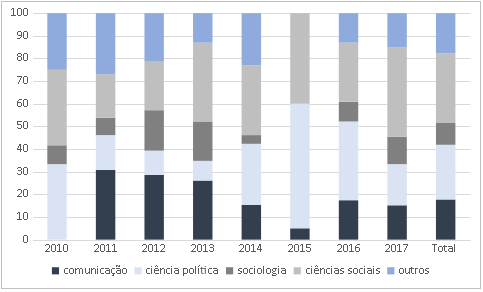
\includegraphics[width=90mm]{./imgs/graf3_4.png}
 \caption{Distribuição da formação de autores\footnotemark}
 \end{figure}

\footnotetext{Fonte: Elaboração dos autores, 2017.}

Outro dado relevante trata das pesquisas interinstitucionais. Dentre os
63 \textit{papers} escritos em parceria, mais da metade conta com
autores da mesma instituição (58,7\%). Em relação ao total de textos,
apenas 24,5\% tem parceria institucional. Esse dado aponta a baixa
relação de pesquisas em rede, as quais demonstrariam parcerias efetivas
entre os grupos de pesquisa.

\begin{comment}
\begin{center}
Tabela 6: Parceria interinstitucional de autores
\end{center}

\begin{center}
\centering
\begin{tabular}{|l|l|l|l|}
\hline
 & \textbf{Frequência} & \textbf{\%} & \textbf{\% Válido} \\ \hline
Não & 37 & 34,9 & 58,7 \\ \hline
Sim & 26 & 24,5 & 41,3 \\ \hline
Total & 63 & -- & 100 \\ \hline
Não se aplica & 43 & 40,6 & -- \\ \hline
Total & 106 & 100 & -- \\ \hline
\end{tabular}
\end{center}

\begin{center}
{\footnotesize\textit{Fonte: Elaboração própria, 2017.}}
\end{center}
\end{comment}

Do mesmo modo, a parceria entre autores de áreas distintas, o que
poderia trazer um ganho qualitativo aos trabalhos ao mesclar teoria e
prática, discussões teóricas convergentes, entre outras possibilidades,
também é algo raro. Isso ocorre em apenas 20,8\% deles. Logo, apesar de
o \textsc{gt} agregar áreas distintas, elas aparentam ainda não conversar entre
si nos artigos. Sendo assim, o \textsc{gt} acaba revelando a pouca relação entre
centros de pesquisa e a pouca convergência entre as áreas, ainda que
elas apareçam nas sessões.

\begin{comment}
\pagebreak
\begin{center}
Tabela 7: Parceria entre autores de diferentes áreas de atuação
\end{center}

\begin{center}
\begin{tabular}{|l|l|l|l|}
\hline
 & \textbf{Frequência} & \textbf{\%} & \textbf{\% Válido} \\ \hline
Não & 41 & 38,7 & 65,1 \\ \hline
Sim & 22 & 20,8 & 34,9 \\ \hline
Total & 63 & 59,4 & 100 \\ \hline
Não se aplica & 43 & 40 & -- \\ \hline
Total & 106 & 100 & -- \\ \hline
\end{tabular}
\end{center}

\begin{center}
{\footnotesize\textit{Fonte: Elaboração própria, 2017.}}
\end{center}
\end{comment}

Passa"-se, a seguir, à análise do conteúdo, propriamente dita, dos
trabalhos.

\section{Características dos trabalhos}

A pesquisa também identificou como os trabalhos se distribuem nas áreas
que compõem o \textsc{gt}, como apresenta o próprio título do grupo:
ciberpolítica, cibercultura e ciberativismo. Assim, 53,8\% deles são
categorizados como ciberpolítica (57), enquanto ciberativismo abrange
28,3\% dos \textit{papers} (30) e cibercultura quase 17,9\% (19).
Constata"-se uma forte presença de estudos sobre \textsc{i\&p}, o
que pode ser relacionado com a presença da Ciência Política como a
segunda área mais presente no \textsc{gt}. Os dados longitudinais mostram algumas
alterações na presença das três subáreas do \textsc{gt}, principalmente o
decréscimo de ciberpolítica, a consolidação do ciberativismo e a perda
de espaço da cibercultura.


 \begin{figure}[!ht]
 \centering
  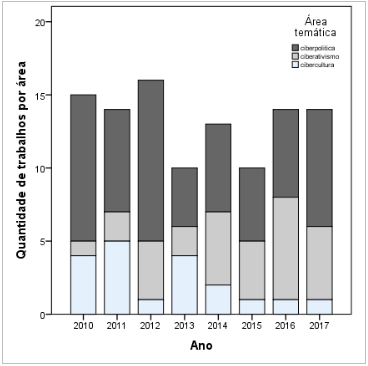
\includegraphics[width=70mm]{./imgs/graf3_5.png}
 \caption{Distribuição temporal das áreas temáticas nos trabalhos do \textsc{gt}\footnotemark}
 \end{figure}

 \footnotetext{Fonte: Elaboração dos autores, 2017.}

Nota"-se como ciberpolítica estava representada na maior parte dos
trabalhos nos três primeiros anos (66,7\% dos 15 totais, 50\% dos 14 e
68,8\% dos 16, em 2010, 2011 e 2012, respectivamente). Depois desses
anos, em 2015 e 2017, volta a aparecer em mais de 50\% dos
\textit{papers}. Nos demais anos, essa temática perde espaço para as
outras áreas, principalmente para ciberativismo, que passa a se destacar
no \textsc{gt}, especialmente a partir de 2014, chegando a 38,5\% dos artigos
apresentados (5 dos 13). Ademais, nota"-se como o predomínio de
ciberativismo acaba ``sufocando'' cibercultura, que é central em apenas
um caso nos anos de 2015, 2016 e 2017.

Outra variável que demonstra como se consolidam e se constroem as
pesquisas apresentadas no \textsc{gt} é a vertente de estudos, social e
institucional, conforme a categorização de Sampaio, Bragatto e Nicolás
(2016). Sobre este ponto, predomina a vertente social que os estudos
sobre a apropriação do uso das \textsc{tic}s pelas organizações da sociedade
civil (59,4\%) ante a institucional com estudos de iniciativas de uso
das \textsc{tic}s por parte das instituições governamentais (40,6\%). Isso chama
atenção, pois os estudos de ciberpolítica, área predominante, estão mais
relacionados às autorias advindas da ciência política, campo que possui,
notadamente, um viés mais institucional em seus estudos. Quando se
relacionam as áreas com as vertentes, todavia, nota"-se que 68,4\% dos
trabalhos de ciberpolítica são da vertente institucional e apenas 31,6\%
da social, o que ainda é notável. Por outro lado, a grande incidência de
uma vertente social está concentrada em ciberativismo --- que tem todos
os trabalhos nesta categoria --- e cibercultura, que apresenta essa
categoria em quase 79\% deles.

Na área social, foram 18 trabalhos na vertente ciberpolítica, 30 em ciberativismo e 15 em cibercultura, totalizando 59,4\% em relação aos trabalhos na área institucional: 39 em ciberpolítica, nenhum em ciberativismo e quatro em cibercultura.

\begin{comment}
\pagebreak

\begin{center}
Tabela 8: Distribuição das áreas temáticas\\ do \textsc{gt} por vertente de estudos\bigskip

\resizebox{\textwidth}{!}{
\begin{tabular}{|l|l|l|l|l|l|}
\hline
 &  & \textbf{Ciberpolítica} & \textbf{Ciberativismo} & \textbf{Cibercultura} & \textbf{Total} \\ \hline
Social & N & 18 & 30 & 15 & 63 \\ \hline
 & \% & 31,6\% & 100\% & 78,9\% & 59,4\% \\ \hline
 & Rp.\,& -2,7 & 2,9 & 1,1 &  \\ \hline
Institucional & N & 39 & 0 & 4 & 43 \\ \hline
 & \% & 68,4\% & 0\% & 21,1\% & 40,6\% \\ \hline
 & Rp.\,& 3,3 & -3,5 & -1,3 &  \\ \hline
Total & N & 57 & 30 & 19 & 106 \\ \hline
 & \% & 100\% & 100\% & 100\% & 100\% \\ \hline
\multicolumn{6}{|l|}{x² = 41.820/ Sig: 0,000} \\ \hline
\end{tabular}
}

{\footnotesize\textit{Fonte: Elaboração própria, 2017.}}
\end{center}
\end{comment}

Aqui, testou"-se a existência de uma tendência de distribuição, o que
gerou um coeficiente \textit{qui"-quadrado} significativo e tendência de
ocorrência positiva significativa\footnote{Ou seja, com resíduos padronizados ---
\textsc{r\,.p.} --- fora do intervalo entre -1,96 e +1,96.} da vertente social para a
área de ciberativismo e negativa para ciberpolítica. O inverso, com
quase os mesmos valores, ocorre em relação à vertente institucional. A
temática cibercultura não apresentou resíduos padronizados
significativos.

Ao observar a perspectiva longitudinal, chamou a atenção o ano de 2011,
em que há poucos trabalhos na vertente social. Em alguns anos,
institucional aparece mais, como 2010 e 2014. No entanto, há, em geral,
um equilíbrio entre as duas categorias, com apenas essa tendência grande
para a vertente social em 2011.

Pode"-se, ainda, observar qual o objeto predominante nos trabalhos. Sobre
isso, tem"-se maior presença das categorias ``instituições'' (27,4\%) e
``movimentos sociais'' (22,6\%), possivelmente, na perspectiva de como
usam tais ferramentas tecnológicas. Apesar de parecer inconsistente ter
mais vertente social e aqui predominarem as instituições, vale observar
a distribuição dos demais tipos de objeto, que podem reunir mais a
perspectiva social que a institucional, como políticas de comunicação,
esfera civil não organizada e sociabilidade, que agregam mais de 40\%
das ocorrências.

Os dados completos, em relação à distribuição dos objetos, são: 29 na categoria instituições; 24 em movimentos sociais e organizações cívicas; 21 em políticas de comunicação (19,8\%), 17 em esfera civil não organizada (16\%), 9 em sociabilidade (8,5\%), 5 em campanhas eleitorais (4,7\%) e um fora dessas categorias (0,9\%).

\begin{comment}
\begin{center}
Tabela 9: Distribuição dos objetos político/social
\end{center}

\begin{center}
\centering
\begin{tabular}{|l|l|l|}
\hline
 & \textbf{N} & \textbf{\%} \\ \hline
Instituições & 29 & 27,4 \\ \hline
Movimentos sociais e org. cívicas & 24 & 22,6 \\ \hline
Políticas de comunicação & 21 & 19,8 \\ \hline
Esfera civil não organizada & 17 & 16 \\ \hline
Sociabilidade & 9 & 8,5 \\ \hline
Campanhas eleitorais & 5 & 4,7 \\ \hline
Outros & 1 & 0,9 \\ \hline
Total & 106 & 100 \\ \hline
\end{tabular}
\end{center}

\begin{center}
{\footnotesize\textit{Fonte: Elaboração própria, 2017.}}
\end{center}
\end{comment}

Nota"-se a baixa presença dos trabalhos sobre campanhas eleitorais
(4,7\%), que têm estudado a apropriação das ferramentas por candidatos,
políticos e partidos no período da disputa eleitoral, que tendem a serem
apresentados no \textsc{gt} de Mídia, Politica e Eleições. Há maior espaço para
estudos sobre instituições, mas fora do aspecto eleitoral.

Para entender melhor o que propriamente tem sido estudado pelos
participantes do \textsc{gt}, há ainda a variável \textit{objeto tecnológico}, como
variável central dos estudos do campo. Ressalta"-se que os objetos
\textit{Internet} e \textit{mídia} são destinados às pesquisas mais gerais, com um
objeto empírico ou pouco definido (normalmente, mais presentes em
reflexões e ensaios sobre os meios no geral) ou muito abrangente (no
caso de estudar simultaneamente vários dos mecanismos apresentados),
categorias que agrupam mais de 43\% das pesquisas apresentadas.

Na categoria objetos tecnológicos, 43 analisam a Internet (40,6\%), 28 as mídias sociais (26,4\%), 20 os \textit{websites} (18,9\%), 4 os fóruns ou chats (3,8\%), 4 os \textit{open source}, \textit{software} livre e dados abertos (3,8\%), 3 a mídia (2,8\%), 3 os blogs (2,8\%), e um os dispositivos móveis (0,9\%).

\begin{comment}
\begin{center}
Tabela 10: Objetos tecnológicos de análise
\end{center}

\begin{center}
\centering
\begin{tabular}{|l|l|l|}
\hline
\textbf{Objeto} & \textbf{N} & \textbf{\%} \\ \hline
Internet & 43 & 40,6 \\ \hline
Mídias Sociais & 28 & 26,4 \\ \hline
Websites & 20 & 18,9 \\ \hline
Fóruns ou chats & 4 & 3,8 \\ \hline
\begin{tabular}[c]{@{}l@{}}Open source, \textit{software}\\ livre e dados abertos\end{tabular} & 4 & 3,8 \\ \hline
Mídia & 3 & 2,8 \\ \hline
Blogs & 3 & 2,8 \\ \hline
Dispositivos móveis & 1 & 0,9 \\ \hline
Total & 106 & 100 \\ \hline
\end{tabular}
\end{center}

\begin{center}
{\footnotesize\textit{Fonte: Elaboração própria, 2017.}}
\end{center}
\end{comment}

Por outro lado, nota"-se a forte presença dos \textit{websites} (18,9\%) e das
mídias sociais (26,4\%) entre os principais objetos. \textit{Blogs},
\textit{chats} e \textit{software} livre, por exemplo, não ganham tanto
destaque no \textsc{gt}. O processo de desenvolvimento tecnológico leva a
constante transformação dos objetos tecnológicos e a consequente
transformação de seus estudos. Desta forma, os estudos sobre blogs e
chats vão perdendo espaço para estudos sobre mídias sociais nos últimos
anos. Essa constante modificação de objeto mostra que a dinâmica da área
está associada com relação entre tecnologia e sociedade.

Outra característica analisada é a abordagem teórica dos textos,
podendo"-se depreender uma abordagem bastante variada sem nenhuma grande
corrente dominando os estudos: 18 sobre Identidade, sociabilidade e cidadania (17\%); 17 em economia política/\,políticas de comunicação (16\%); 16 em participação (15,1\%); 14 em engajamento (13,2\%); 13 em \textit{accountability} (12,3\%); sete em estratégia política e eleitoral (6,6\%); cinco em deliberação (4,7\%); cinco em jornalismo político (4,7\%); quatro em transparência e informação (3,8\%); três em inclusão digital (2,8\%); um em capital social e cultura política (0,9\%); e três que não sei encaixam nessas categorias.

Apesar de abordagens variadas entre os trabalhos, percebem"-se algumas
menos frequentes, como jornalismo político (4,7\%). Isso se deve,
provavelmente, à menor procura dos autores que trazem esta
discussão pelo \textsc{gt}, já que há outros espaços na \textsc{\textsc{anpocs}} para discussões
mais centradas em mídia e política. Deliberação, apesar do grande
destaque que recebe na literatura, também aparece menos no \textsc{gt} (4,7\%).
Por outro lado, chama atenção a preocupação dos estudos com a economia
política e as políticas de comunicação.

Um avanço importante que mostra a consolidação dos estudos do \textsc{gt} é que
predominam os trabalhos empíricos, com 88\% do total, sendo somente 17\%
teóricos. No entanto, como o Grupo tem três subáreas, é importante
observar como essa constatação pode ser apropriada por cada uma delas.

Dos 18 \textit{papers} teóricos, seis são sobre ciberpolítica, cinco sobre ciberativismo e sete sobre cibercultura. Dos 88 empíricos, 51 são sobre ciberpolítica, 25 sobre ciberativismo e 12 sobre cibercultura.

\begin{comment}
\begin{center}
Tabela 12: Tipo de estudo x Área temática do \textsc{gt}
\end{center}

%\begin{center}
%\centering
%\begin{tabular}{|c|l|l|l|l|l|}
%\hline
%\multicolumn{2}{|l|}{\multirow{2}{*}{}} & \multicolumn{3}{c|}{\textbf{Área temática}} & \%multicolumn{1}{c|}{\multirow{2}{*}{\textbf{Total}}} \\ \cline{3-5}
%\multicolumn{2}{|l|}{} & \textbf{\begin{tabular}[c]{@{}l@{}}Ciber-\\ política\end{tabular}} & \textbf{\begin{tabular}[c]{@{}l@{}}Ciber-\\ ativismo\end{tabular}} & \textbf{\begin{%tabular}[c]{@{}l@{}}Ciber-\\ cultura\end{tabular}} & \multicolumn{1}{c|}{} \\ \hline
%\multirow{2}{*}{\textbf{\begin{tabular}[c]{@{}c@{}}Tipos de\\ estudo\end{tabular}}} & \%textbf{teórico} & 6 & 5 & 7 & 18 \\ \cline{2-6} 
 %& \textbf{empírico} & 51 & 25 & 12 & 88 \\ \hline
%\multicolumn{2}{|c|}{\textbf{Total}} & 57 & 30 & 19 & 106 \\ \hline
%\end{tabular}
%\end{center}

\begin{center}
{\footnotesize\textit{Fonte: Elaboração própria, 2017.}}
\end{center}
\end{comment}

Percebe"-se que dos 57 \textit{papers} de ciberpolítica, apenas
6 deles são teóricos, o que equivale a 10,5\%. Já no caso de
ciberativismo, entre os 30 trabalhos, cinco possuem uma abordagem
teórica, alcançando o percentual de 16\%. No caso de cibercultura, os
sete artigos teóricos chegam a 36,8\% do total da subárea, que já tende
a ser minoria no \textsc{gt}, conforme discutido anteriormente. Sendo assim, é a
guinada da ciberpolítica e ciberativismo que leva mais empiria ao \textsc{gt}.

Na sequência, observa"-se o método de pesquisa utilizado nas pesquisas.
Destaca"-se a predominância de abordagem qualitativa, com 49 trabalhos (46,2\%) sobre a
quantitativa, com 25 trabalhos (23,6\%), enquanto reflexões teóricas bibliográficas vem em
seguida com 18 trabalhos (17\%). Outro ponto a se destacar é que 13,2\% dos trabalhos
apresentados, totalizando 14, foram categorizados como método misto por utilizarem as
abordagens qualitativa e quantitativa.

\begin{comment}
\begin{center}
Tabela 13: Distribuição por tipo de método
\end{center}

\begin{center}
\centering
\begin{tabular}{|l|l|l|}
\hline
 & \textbf{N} & \textbf{\%} \\ \hline
Qualitativo & 49 & 46,2 \\ \hline
Quantitativo & 25 & 23,6 \\ \hline
Bibliográfico & 18 & 17 \\ \hline
Quanti./Quali. & 14 & 13,2 \\ \hline
Total & 106 & 100 \\ \hline
\end{tabular}
\end{center}

\begin{center}
{\footnotesize\textit{Fonte: Elaboração própria, 2017.}}
\end{center}
\end{comment}

De modo mais específico observam"-se as técnicas de pesquisa
predominantes. Retirando os 18 trabalhos que não são empíricos (16,3\%),
50\% dos demais fazem análise de conteúdo. Nota"-se que, apesar da
vertente qualitativa predominar no \textsc{gt}, há pouca apropriação de
entrevistas, grupos focais e métodos de interação direta com o objeto de
pesquisa, como etnografia.

Além da centralidade da análise de conteúdo em 50\% dos trabalhos,
percebe"-se que nenhuma outra técnica se sobressai, havendo, inclusive,
poucos que se utilizam de análise do discurso (1,1\%), por exemplo. Há
\textit{papers} que, apesar de se proporem à empiria, não apresentam um
método específico de análise passível de se enquadrar entre os
principais, o que chegou a 5,7\% deles. Por outro lado, percebe"-se a
entrada de novas técnicas, tal como a análise de redes, que obteve
quatro ocorrências. As demais técnicas observadas foram: entrevista e grupo focal, com 12 ocorrências (11,3\%); análise documental, com seis (5,7\%); etnografia/\,observação
participante e pesquisa ação, com cinco (4,7\%); e \textit{survey}, com um (0,9\%).

\begin{comment}
\begin{center}
Tabela 14: Técnicas de pesquisa utilizadas
\end{center}

\begin{center}
\centering
\begin{tabular}{|l|l|l|l|}
\hline
 & \textbf{N} & \textbf{\%} & \textbf{\% válido} \\ \hline
Análise de conteúdo & 53 & 50 & 60,2 \\ \hline
Entrevista e grupo focal & 12 & 11,3 & 13,6 \\ \hline
Análise documental & 6 & 5,7 & 6,8 \\ \hline
Indefinido & 6 & 5,7 & 6,8 \\ \hline
\begin{tabular}[c]{@{}l@{}}Etnografia/observação\\ participante e pesquisa ação\end{tabular} & 5 & 4,7 & 5,7 \\ \hline
Análise de redes & 4 & 3,8 & 4,5 \\ \hline
Survey & 1 & 0,9 & 1,1 \\ \hline
Análise do discurso & 1 & 0,9 & 1,1 \\ \hline
Total & 88 & 83 & 100 \\ \hline
Não se aplica & 18 & 17 &  \\ \hline
Total & 106 & 100 &  \\ \hline
\end{tabular}
\end{center}

\begin{center}
{\footnotesize\textit{Fonte: Elaboração própria, 2017.}}
\end{center}
\end{comment}

Outra característica observada é o uso da estatística, que aparece em 50
artigos (47,2\%), a partir de testes variados dentro do escopo do
método: 41 casos de frequência simples (38,7\%); três de estatística univariada (2,8\%); seis de estatística bivariada (5,7\%); e 56 que não se aplicam (52,8\%).

\begin{comment}
\begin{center}
Tabela 15: Tipo de estatística utilizada
\end{center}

\begin{center}
\centering
\begin{tabular}{|l|l|l|l|}
\hline
 & \textbf{N} & \textbf{\%} & \textbf{\% válido} \\ \hline
Frequência simples & 41 & 38,7 & 82 \\ \hline
Estatística univariada & 3 & 2,8 & 6 \\ \hline
Estatística bivariada & 6 & 5,7 & 12 \\ \hline
Total & 50 & 47,2 & 100 \\ \hline
Não se aplica & 56 & 52,8 &  \\ \hline
Total & 106 & 100 &  \\ \hline
\end{tabular}
\end{center}

\begin{center}
{\footnotesize\textit{Fonte: Elaboração própria, 2017.}}
\end{center}
\end{comment}

Nota"-se, entretanto, que não há avanços significativos com a utilização
desse recurso analítico, pois prevalece de maneira significativa o uso
de frequências simples, o que aponta para um caráter mais descritivo dos
trabalhos.

\section{Considerações finais}

O estudo sobre a produção apresentada no \textsc{gt} Ciberpolítica, Ciberativismo
e Cibercultura permitiu identificar algumas características da área,
que, embora ainda em formação, começa a delinear suas especificidades. O
objetivo da proposta foi mapear o perfil das pesquisas apresentadas
durante os oito anos do \textsc{gt}, o que traz indicativos de como essa área
multitemática tem se estruturado ao longo do tempo.

A análise permite afirmar que as pesquisas apresentadas no \textsc{gt}, com quase
50\% de todos os trabalhos apresentados possuindo apenas um autor ou
autora, possivelmente, não são o resultado de investigação coletiva ou
de grupos de pesquisa que, normalmente, contam com um processo
colaborativo de produção. O trabalho de Sampaio, Bragatto e Nicolás
(2016) segue os mesmos achados, o que demonstra que essa é uma prática
comum na área, uma vez que a pesquisa mencionada trabalha com eventos de
todo o campo de Comunicação e Política. Este comportamento, todavia, é
contrário àquilo que tende a ocorrer atualmente nas Ciências Humanas de
modo generalizado, que nos últimos 20 anos saltou de 2\% para 40\% em
média, como indica Codato \textit{et al.} (2017), no que diz respeito aos
trabalhos em coautoria.

Apesar da intrínseca característica interdisciplinar do grupo, com
participantes de diversas áreas do conhecimento, por fazer parte de um
congresso de ciências sociais, sua composição tem uma maioria de
participantes do próprio campo de sociais, notadamente da ciência
política, indicando um viés mais próximo dos estudos sobre Internet e
política, como pode ser observado pela maior ocorrência de artigos de
ciberpolítica. Esse perfil também pode estar associado à formação dos
primeiros coordenadores do \textsc{gt}, oriundos da ciência política, seja pela
formação ou área de produção atual.

Constata"-se, ainda, que houve uma grande concentração dos trabalhos
apresentados em poucas instituições, especialmente do eixo Sul"-Sudeste.
Isso pode indicar que o \textsc{gt} precisa estar mais atento à diversidade a ser
contemplada quando da avaliação dos \textit{papers} submetidos, uma vez
que, há alguns anos, grupos de pesquisa que abordam essa interface têm
se formado nas regiões Norte e Centro"-Oeste, aquelas menos contempladas
no \textsc{gt}, e ganhado alguma proeminência nacional. É surpreendente a redução
de participação de instituições do Nordeste nesse grupo, uma vez que, no
campo de \textsc{i\&p}, a região é muito atuante (\textsc{sampaio,
bragatto \& nicolás}, 2016), o que possivelmente pode ser explicado pela
maior parte dos autores dessa região ser da área de comunicação e
não das ciências sociais.

Não se pode deixar de perceber a menor participação e permanência de
mulheres no \textsc{gt}. Esse fato segue em movimento contrário àquele de
crescimento das mulheres no setor científico no Brasil, iniciado na
década de 1980 (\textsc{leta}, 2003) e intensificado, especialmente, nos últimos
anos, quando as mulheres atingiram a marca de 49\% da autoria de
trabalhos acadêmicos no país (\textsc{elsevier}, 2017).

Por fim, pode"-se apontar que, em suma, os estudos têm se caracterizado
nos últimos anos como mais empíricos, preocupados em compreender
fenômenos políticos, especialmente quanto à sua relação com os
\textit{media} digitais. Eles, todavia, continuam em um nível mais
descritivo de observação, o que indica uma tentativa de mapeamento dos
casos a partir de uma análise de conteúdo de diferentes mecanismos com
maior foco nas instituições do Estado, especialmente o parlamento, e na
sociedade civil organizada, achados que corroboram os resultados de
Sampaio, Bragatto e Nicolás (2016).

Diferentemente de outras áreas da ciência política, contudo, o viés
institucional não é a principal vertente nos estudos apresentados no \textsc{gt},
havendo certo equilíbrio com o viés social, que apresenta, inclusive,
uma maior ocorrência. Dessa forma, os estudos de caráter
predominantemente empírico mostram uma pluralidade de objetos de
pesquisa com maior ênfase nas instituições, movimentos sociais e
políticas de comunicação. Percebe"-se a diversidade de abordagens, como
questões de identidade, sociabilidade, cidadania, engajamento, economia
política, \textit{accountability}, entre outros.

Essas características denotam a especificidade do campo de estudos sobre
Internet, que se caracterizam por permitir formas de mobilização/\,ação
institucionais e não institucionais que envolvem aspectos não só
políticos, mas também sociais, culturais e tecnológicos. Assim, como o
desenvolvimento de novas tecnologias digitais (\textit{softwares},
plataformas, mídias sociais, etc.) e diferentes formas de apropriação e
uso dessas tecnologias, o campo produz inovações e novos desafios aos
pesquisadores.

Esses resultados também permitem observar algumas lacunas que podem
indicar novas agendas de pesquisa. Além do incentivo de uma maior
pluralidade de autoras e de instituições presentes nas diferentes
regiões do Brasil, o estudo também destaca a necessidade de um maior
cuidado metodológico. Por um lado, detecta"-se uma reduzida gama de
técnicas empregadas, concentradas em análise de conteúdo e, geralmente,
apenas com estatística descritiva básica (algo aparentemente geral da
área de \textsc{i\&p}, como apontado pelo estudo de Sampaio e colegas, 2016),
enquanto, é notável, que os meios digitais, em sua constante e rápida
evolução, estão constantemente demandando novas técnicas de averiguação
e os cuidados com questões específicas a esses meios (\textit{e.\,g}. robôs usados
para divulgar candidatos e/\,ou ideias, páginas divulgando \textit{fake
news}, ou até os algoritmos que regem as mídias sociais).

Com a possibilidade da mineração e análise de altos volumes de
informação (\textit{i.\,e.} \textit{Big Data}), as técnicas estatísticas e de análise de
redes deveriam receber cada vez mais atenção e refinamento. Isso, por
outro lado, não deve significar o abandono das técnicas de pesquisa
tradicionais. Afinal, as pesquisas não podem se centrar exclusivamente
no conteúdo das plataformas digitais, mas devem estar atentas a seus
criadores, hospedeiros e usuários, o que reforça o uso de entrevistas,
\textit{surveys}, grupos focais e mesmo etnografias (com as devidas
adaptações aos meios em questão). É justamente nesse sentido que uma
maior interdisciplinaridade e mais coautorias parecem ser um caminho
frutífero para tais avanços.

Em especial, é preciso reconhecer que a dinâmica informacional, o rápido
desenvolvimento tecnológico e as diferentes formas de apropriação das
tecnologias de informação e comunicação fazem com que a área esteja
sempre se reconfigurando, surgindo novos objetos de estudo, novos
problemas e novas ferramentas de pesquisa que visam explicar um fenômeno
complexo e em constante transformação, sempre aberto para inovadoras
formas de estudo nas Ciências Sociais.

Diante de tal desafio, o que se pode concluir, enfim, é que, apesar de
alguns ajustes ainda serem necessários, o \textsc{gt} estudado tem auxiliado no
desenvolvimento de um campo interdisciplinar de estudos, apresentando
avanços e se constituindo como um importante espaço para o
fortalecimento das pesquisas.

\begin{bibliohedra}
\tit{albuquerque}, Afonso. ``Notas para uma agenda da pesquisa sobre a
propaganda política na televisão no Brasil''. \textit{Revista \textit{Eco}}, Rio de Janeiro, v.\,12, p.\,4--10, 2010.

\tit{amaral}, Adriana e \textsc{montardo}, Sandra Portella. ``Mapeamento
Temático da História da Cibercultura no Brasil''. \textit{Anais do \textsc{xxxv} Congresso
Brasileiro de Ciências da Comunicação, Fortaleza}. São Paulo: Intercom, v.\,1, 1--17, 2012.

\tit{araújo}, Rafael de Paula Aguiar; \textsc{penteado}, Cláudio Luis Camargo; \textsc{dos
santos}, Marcelo Burgos Pimentel. ``Democracia digital e
experiências de e"-participação: webativismo e políticas públicas''.
\textit{História, Ciências, Saúde"-Manguinhos}, v.\,22, p.\,1597--1619, 2015.

\tit{castells}, Manuel. \textit{Redes de indignação e esperança:
movimentos sociais na era da Internet.} Rio de Janeiro: Zahar, 2017.

\titidem. \textit{A Galáxia Internet: reflexões sobre a
Internet, negócios e a sociedade}. Rio de Janeiro: Zahar, 2003.

\titidem. \textit{A era da informação: economia, sociedade
e cultura}. São Paulo: Paz e Terra, 1999.

\tit{codato}, Adriano \textit{et a.}
``A colaboração na Ciência Política brasileira: um estudo
exploratório do padrão de coautorias em periódicos nacionais''.
\textit{Paper apresentado no 9º Congresso da \textsc{alacip}}, Montevidéu,
Uruguai, 2017.

\tit{dias}, Marcia Ribeiro. ``Nas brumas do \textsc{hgpe}: a imagem partidária
nas campanhas presidenciais brasileiras (1989 a 2010)''. \textit{Opinião
Pública}, v.\,19, n.\,1, p.\,198--219, 2013.

\tit{elsevier}. ``Gender in the Global Research Landscape''. \textit{Analysis of
research performance through a gender lens across 20 years, 12
geographies, and 27 subject areas}, 2017. 

\tit{figueiredo}, Marcus \textit{et al.}
``Estratégias de persuasão eleitoral: uma proposta metodológica
para o estudo da propaganda eleitoral''. \textit{Opinião Pública}, v.\,4,
n.\,3, p.\,182--203, 1997.

\tit{gomes}, Wilson. ``20 anos de política, Estado e democracia digitais: uma
cartografia do campo''. \textit{In}: \textsc{silva}, Sivaldo Pereira; \textsc{bragatto}, Rachel Callai; \textsc{sampaio}, Rafael Cardoso (org.). \textit{Democracia
digital, comunicação política e redes: teoria e prática}. Rio
de Janeiro: Letra \& Imagem, p.\,25--45, 2016.

\titidem. \textit{Transformação da política na era da
comunicação de massa}. São Paulo: Paulus, 2004.

\tit{harlow}, Summer; \textsc{harp}, Dustin. ``Collective action on the Web: A
cross"-cultural study of social networking sites and online and offline
activism in the United States and Latin America''. \textit{Information,
Communication \& Society}, v.\,15, n\,.2, p.\,196--216, 2012.

\tit{lemos}, André. \textit{Cibercultura: tecnologia e vida social na
cultura contemporânea}. Porto Alegre: Sulina, 2002.

\titidem\mbox{} e \textsc{lévy}, Pierre. \textit{O futuro da Internet: em
direção a uma ciberdemocracia planetária}. São Paulo: Paulus, 2010.

\tit{leta}, Jacqueline. ``As mulheres na ciência brasileira:
crescimento, contrastes e um perfil de sucesso''. \textit{Estudos
avançados}, v.\,17, n.\,49, p.\,271--284, 2003.

\tit{lévy}, Pierre. \textit{Cibercultura}. São Paulo: Editora 34, 1999.

\tit{lima}, Venício. ``Revisitando sete teses sobre mídia e política
no Brasil''. \textit{Comunicação \& Sociedade}, v.\,30, n.\,51, p.\,13--33, 2009.

\tit{miguel}, Luis Felipe e \textsc{biroli}, Flávia. ``Comunicação e política: um campo
de estudos e seus desdobramentos no Brasil''. \textit{In}: \line(1,0){25} e
\line(1,0){25} (org.). \textit{Mídia, representação e democracia}.
São Paulo: Editora Hucitec, p.\,7--24, 2010.

\tit{panke}, Luciana; \textsc{cervi}, Emerson. ``Análise da comunicação
eleitoral: uma proposta metodológica para os estudos do \textsc{hgpe}''.
\textit{Revista Contemporânea}, Salvador, v.\,9, n.\,3, p.\,390--404, 2011.

\tit{rubim}, Antonio Albino Canelas; \textsc{azevedo}, Fernando Antonio.
``Mídia e política no Brasil: textos e agenda de pesquisa''. \textit{Lua
Nova}, v.\,43, p.\,189--216, 1998.

\tit{sampaio}, Rafael Cardoso; \textsc{bragatto}, Rachel Callai; \textsc{nicolás}, Maria
Alejandra. ``A construção do campo de Internet e política:
análise dos artigos brasileiros apresentados entre 2000 e 2014''.
\textit{Revista Brasileira de Ciência Política}, v.\,21, p.\,287--322, 2016.

\tit{silveira}, Sergio Amadeu da. ``Ciberativismo, cultura hacker e o
individualismo colaborativo''. \textit{Revista \textsc{usp}}, v.\,86, p.\,28--39, 2010.

\tit{weber}, Maria Helena. ``O estatuto da Imagem Pública na disputa
política''. \textit{Revista Eco}, Rio de Janeiro, v.\,12, n.\,3, p.\,79--94, 2009.
\end{bibliohedra}
